\documentclass[twoside]{book}

% Packages required by doxygen
\usepackage{calc}
\usepackage{doxygen}
\usepackage{graphicx}
\usepackage[utf8]{inputenc}
\usepackage{makeidx}
\usepackage{multicol}
\usepackage{multirow}
\usepackage{fixltx2e}
\PassOptionsToPackage{warn}{textcomp}
\usepackage{textcomp}
\usepackage[nointegrals]{wasysym}
\usepackage[table]{xcolor}

% Font selection
\usepackage[T1]{fontenc}
\usepackage{mathptmx}
\usepackage[scaled=.90]{helvet}
\usepackage{courier}
\usepackage{amssymb}
\usepackage{sectsty}
\renewcommand{\familydefault}{\sfdefault}
\allsectionsfont{%
  \fontseries{bc}\selectfont%
  \color{darkgray}%
}
\renewcommand{\DoxyLabelFont}{%
  \fontseries{bc}\selectfont%
  \color{darkgray}%
}
\newcommand{\+}{\discretionary{\mbox{\scriptsize$\hookleftarrow$}}{}{}}

% Page & text layout
\usepackage{geometry}
\geometry{%
  a4paper,%
  top=2.5cm,%
  bottom=2.5cm,%
  left=2.5cm,%
  right=2.5cm%
}
\tolerance=750
\hfuzz=15pt
\hbadness=750
\setlength{\emergencystretch}{15pt}
\setlength{\parindent}{0cm}
\setlength{\parskip}{0.2cm}
\makeatletter
\renewcommand{\paragraph}{%
  \@startsection{paragraph}{4}{0ex}{-1.0ex}{1.0ex}{%
    \normalfont\normalsize\bfseries\SS@parafont%
  }%
}
\renewcommand{\subparagraph}{%
  \@startsection{subparagraph}{5}{0ex}{-1.0ex}{1.0ex}{%
    \normalfont\normalsize\bfseries\SS@subparafont%
  }%
}
\makeatother

% Headers & footers
\usepackage{fancyhdr}
\pagestyle{fancyplain}
\fancyhead[LE]{\fancyplain{}{\bfseries\thepage}}
\fancyhead[CE]{\fancyplain{}{}}
\fancyhead[RE]{\fancyplain{}{\bfseries\leftmark}}
\fancyhead[LO]{\fancyplain{}{\bfseries\rightmark}}
\fancyhead[CO]{\fancyplain{}{}}
\fancyhead[RO]{\fancyplain{}{\bfseries\thepage}}
\fancyfoot[LE]{\fancyplain{}{}}
\fancyfoot[CE]{\fancyplain{}{}}
\fancyfoot[RE]{\fancyplain{}{\bfseries\scriptsize Generated on Thu Sep 18 2014 15\+:52\+:00 for L\+M\+F library by Doxygen }}
\fancyfoot[LO]{\fancyplain{}{\bfseries\scriptsize Generated on Thu Sep 18 2014 15\+:52\+:00 for L\+M\+F library by Doxygen }}
\fancyfoot[CO]{\fancyplain{}{}}
\fancyfoot[RO]{\fancyplain{}{}}
\renewcommand{\footrulewidth}{0.4pt}
\renewcommand{\chaptermark}[1]{%
  \markboth{#1}{}%
}
\renewcommand{\sectionmark}[1]{%
  \markright{\thesection\ #1}%
}

% Indices & bibliography
\usepackage{natbib}
\usepackage[titles]{tocloft}
\setcounter{tocdepth}{3}
\setcounter{secnumdepth}{5}
\makeindex

% Hyperlinks (required, but should be loaded last)
\usepackage{ifpdf}
\ifpdf
  \usepackage[pdftex,pagebackref=true]{hyperref}
\else
  \usepackage[ps2pdf,pagebackref=true]{hyperref}
\fi
\hypersetup{%
  colorlinks=true,%
  linkcolor=blue,%
  citecolor=blue,%
  unicode%
}

% Custom commands
\newcommand{\clearemptydoublepage}{%
  \newpage{\pagestyle{empty}\cleardoublepage}%
}


%===== C O N T E N T S =====

\begin{document}

% Titlepage & ToC
\hypersetup{pageanchor=false,
             bookmarks=true,
             bookmarksnumbered=true,
             pdfencoding=unicode
            }
\pagenumbering{roman}
\begin{titlepage}
\vspace*{7cm}
\begin{center}%
{\Large L\+M\+F library }\\
\vspace*{1cm}
{\large Generated by Doxygen 1.8.7}\\
\vspace*{0.5cm}
{\small Thu Sep 18 2014 15:52:00}\\
\end{center}
\end{titlepage}
\clearemptydoublepage
\tableofcontents
\clearemptydoublepage
\pagenumbering{arabic}
\hypersetup{pageanchor=true}

%--- Begin generated contents ---
\chapter{Namespace Index}
\section{Packages}
Here are the packages with brief descriptions (if available)\+:\begin{DoxyCompactList}
\item\contentsline{section}{\hyperlink{namespacelmf}{lmf} }{\pageref{namespacelmf}}{}
\item\contentsline{section}{\hyperlink{namespacelmf_1_1src}{lmf.\+src} }{\pageref{namespacelmf_1_1src}}{}
\item\contentsline{section}{\hyperlink{namespacelmf_1_1src_1_1common}{lmf.\+src.\+common} }{\pageref{namespacelmf_1_1src_1_1common}}{}
\item\contentsline{section}{\hyperlink{namespacelmf_1_1src_1_1common_1_1range}{lmf.\+src.\+common.\+range} }{\pageref{namespacelmf_1_1src_1_1common_1_1range}}{}
\item\contentsline{section}{\hyperlink{namespacelmf_1_1src_1_1config}{lmf.\+src.\+config} }{\pageref{namespacelmf_1_1src_1_1config}}{}
\item\contentsline{section}{\hyperlink{namespacelmf_1_1src_1_1config_1_1mdf}{lmf.\+src.\+config.\+mdf} }{\pageref{namespacelmf_1_1src_1_1config_1_1mdf}}{}
\item\contentsline{section}{\hyperlink{namespacelmf_1_1src_1_1config_1_1tex}{lmf.\+src.\+config.\+tex} }{\pageref{namespacelmf_1_1src_1_1config_1_1tex}}{}
\item\contentsline{section}{\hyperlink{namespacelmf_1_1src_1_1core}{lmf.\+src.\+core} }{\pageref{namespacelmf_1_1src_1_1core}}{}
\item\contentsline{section}{\hyperlink{namespacelmf_1_1src_1_1core_1_1definition}{lmf.\+src.\+core.\+definition} }{\pageref{namespacelmf_1_1src_1_1core_1_1definition}}{}
\item\contentsline{section}{\hyperlink{namespacelmf_1_1src_1_1core_1_1form}{lmf.\+src.\+core.\+form} }{\pageref{namespacelmf_1_1src_1_1core_1_1form}}{}
\item\contentsline{section}{\hyperlink{namespacelmf_1_1src_1_1core_1_1form__representation}{lmf.\+src.\+core.\+form\+\_\+representation} }{\pageref{namespacelmf_1_1src_1_1core_1_1form__representation}}{}
\item\contentsline{section}{\hyperlink{namespacelmf_1_1src_1_1core_1_1global__information}{lmf.\+src.\+core.\+global\+\_\+information} }{\pageref{namespacelmf_1_1src_1_1core_1_1global__information}}{}
\item\contentsline{section}{\hyperlink{namespacelmf_1_1src_1_1core_1_1lexical__entry}{lmf.\+src.\+core.\+lexical\+\_\+entry} }{\pageref{namespacelmf_1_1src_1_1core_1_1lexical__entry}}{}
\item\contentsline{section}{\hyperlink{namespacelmf_1_1src_1_1core_1_1lexical__resource}{lmf.\+src.\+core.\+lexical\+\_\+resource} }{\pageref{namespacelmf_1_1src_1_1core_1_1lexical__resource}}{}
\item\contentsline{section}{\hyperlink{namespacelmf_1_1src_1_1core_1_1lexicon}{lmf.\+src.\+core.\+lexicon} }{\pageref{namespacelmf_1_1src_1_1core_1_1lexicon}}{}
\item\contentsline{section}{\hyperlink{namespacelmf_1_1src_1_1core_1_1representation}{lmf.\+src.\+core.\+representation} }{\pageref{namespacelmf_1_1src_1_1core_1_1representation}}{}
\item\contentsline{section}{\hyperlink{namespacelmf_1_1src_1_1core_1_1sense}{lmf.\+src.\+core.\+sense} }{\pageref{namespacelmf_1_1src_1_1core_1_1sense}}{}
\item\contentsline{section}{\hyperlink{namespacelmf_1_1src_1_1core_1_1statement}{lmf.\+src.\+core.\+statement} }{\pageref{namespacelmf_1_1src_1_1core_1_1statement}}{}
\item\contentsline{section}{\hyperlink{namespacelmf_1_1src_1_1core_1_1text__representation}{lmf.\+src.\+core.\+text\+\_\+representation} }{\pageref{namespacelmf_1_1src_1_1core_1_1text__representation}}{}
\item\contentsline{section}{\hyperlink{namespacelmf_1_1src_1_1input}{lmf.\+src.\+input} }{\pageref{namespacelmf_1_1src_1_1input}}{}
\item\contentsline{section}{\hyperlink{namespacelmf_1_1src_1_1input_1_1elan}{lmf.\+src.\+input.\+elan} }{\pageref{namespacelmf_1_1src_1_1input_1_1elan}}{}
\item\contentsline{section}{\hyperlink{namespacelmf_1_1src_1_1input_1_1ite}{lmf.\+src.\+input.\+ite} }{\pageref{namespacelmf_1_1src_1_1input_1_1ite}}{}
\item\contentsline{section}{\hyperlink{namespacelmf_1_1src_1_1input_1_1mdf}{lmf.\+src.\+input.\+mdf} }{\pageref{namespacelmf_1_1src_1_1input_1_1mdf}}{}
\item\contentsline{section}{\hyperlink{namespacelmf_1_1src_1_1input_1_1toolbox__settings}{lmf.\+src.\+input.\+toolbox\+\_\+settings} }{\pageref{namespacelmf_1_1src_1_1input_1_1toolbox__settings}}{}
\item\contentsline{section}{\hyperlink{namespacelmf_1_1src_1_1input_1_1txt}{lmf.\+src.\+input.\+txt} }{\pageref{namespacelmf_1_1src_1_1input_1_1txt}}{}
\item\contentsline{section}{\hyperlink{namespacelmf_1_1src_1_1input_1_1xls}{lmf.\+src.\+input.\+xls} }{\pageref{namespacelmf_1_1src_1_1input_1_1xls}}{}
\item\contentsline{section}{\hyperlink{namespacelmf_1_1src_1_1input_1_1xml__lmf}{lmf.\+src.\+input.\+xml\+\_\+lmf} }{\pageref{namespacelmf_1_1src_1_1input_1_1xml__lmf}}{}
\item\contentsline{section}{\hyperlink{namespacelmf_1_1src_1_1morphology}{lmf.\+src.\+morphology} }{\pageref{namespacelmf_1_1src_1_1morphology}}{}
\item\contentsline{section}{\hyperlink{namespacelmf_1_1src_1_1morphology_1_1component}{lmf.\+src.\+morphology.\+component} }{\pageref{namespacelmf_1_1src_1_1morphology_1_1component}}{}
\item\contentsline{section}{\hyperlink{namespacelmf_1_1src_1_1morphology_1_1lemma}{lmf.\+src.\+morphology.\+lemma} }{\pageref{namespacelmf_1_1src_1_1morphology_1_1lemma}}{}
\item\contentsline{section}{\hyperlink{namespacelmf_1_1src_1_1morphology_1_1list__of__components}{lmf.\+src.\+morphology.\+list\+\_\+of\+\_\+components} }{\pageref{namespacelmf_1_1src_1_1morphology_1_1list__of__components}}{}
\item\contentsline{section}{\hyperlink{namespacelmf_1_1src_1_1morphology_1_1related__form}{lmf.\+src.\+morphology.\+related\+\_\+form} }{\pageref{namespacelmf_1_1src_1_1morphology_1_1related__form}}{}
\item\contentsline{section}{\hyperlink{namespacelmf_1_1src_1_1morphology_1_1stem}{lmf.\+src.\+morphology.\+stem} }{\pageref{namespacelmf_1_1src_1_1morphology_1_1stem}}{}
\item\contentsline{section}{\hyperlink{namespacelmf_1_1src_1_1morphology_1_1word__form}{lmf.\+src.\+morphology.\+word\+\_\+form} }{\pageref{namespacelmf_1_1src_1_1morphology_1_1word__form}}{}
\item\contentsline{section}{\hyperlink{namespacelmf_1_1src_1_1morphosyntax}{lmf.\+src.\+morphosyntax} }{\pageref{namespacelmf_1_1src_1_1morphosyntax}}{}
\item\contentsline{section}{\hyperlink{namespacelmf_1_1src_1_1morphosyntax_1_1paradigm}{lmf.\+src.\+morphosyntax.\+paradigm} }{\pageref{namespacelmf_1_1src_1_1morphosyntax_1_1paradigm}}{}
\item\contentsline{section}{\hyperlink{namespacelmf_1_1src_1_1mrd}{lmf.\+src.\+mrd} }{\pageref{namespacelmf_1_1src_1_1mrd}}{}
\item\contentsline{section}{\hyperlink{namespacelmf_1_1src_1_1mrd_1_1context}{lmf.\+src.\+mrd.\+context} }{\pageref{namespacelmf_1_1src_1_1mrd_1_1context}}{}
\item\contentsline{section}{\hyperlink{namespacelmf_1_1src_1_1mrd_1_1equivalent}{lmf.\+src.\+mrd.\+equivalent} }{\pageref{namespacelmf_1_1src_1_1mrd_1_1equivalent}}{}
\item\contentsline{section}{\hyperlink{namespacelmf_1_1src_1_1mrd_1_1subject__field}{lmf.\+src.\+mrd.\+subject\+\_\+field} }{\pageref{namespacelmf_1_1src_1_1mrd_1_1subject__field}}{}
\item\contentsline{section}{\hyperlink{namespacelmf_1_1src_1_1output}{lmf.\+src.\+output} }{\pageref{namespacelmf_1_1src_1_1output}}{}
\item\contentsline{section}{\hyperlink{namespacelmf_1_1src_1_1output_1_1doc}{lmf.\+src.\+output.\+doc} }{\pageref{namespacelmf_1_1src_1_1output_1_1doc}}{}
\item\contentsline{section}{\hyperlink{namespacelmf_1_1src_1_1output_1_1html}{lmf.\+src.\+output.\+html} }{\pageref{namespacelmf_1_1src_1_1output_1_1html}}{}
\item\contentsline{section}{\hyperlink{namespacelmf_1_1src_1_1output_1_1mdf}{lmf.\+src.\+output.\+mdf} }{\pageref{namespacelmf_1_1src_1_1output_1_1mdf}}{}
\item\contentsline{section}{\hyperlink{namespacelmf_1_1src_1_1output_1_1tex}{lmf.\+src.\+output.\+tex} }{\pageref{namespacelmf_1_1src_1_1output_1_1tex}}{}
\item\contentsline{section}{\hyperlink{namespacelmf_1_1src_1_1output_1_1txt}{lmf.\+src.\+output.\+txt} }{\pageref{namespacelmf_1_1src_1_1output_1_1txt}}{}
\item\contentsline{section}{\hyperlink{namespacelmf_1_1src_1_1output_1_1xls}{lmf.\+src.\+output.\+xls} }{\pageref{namespacelmf_1_1src_1_1output_1_1xls}}{}
\item\contentsline{section}{\hyperlink{namespacelmf_1_1src_1_1output_1_1xml__ite}{lmf.\+src.\+output.\+xml\+\_\+ite} }{\pageref{namespacelmf_1_1src_1_1output_1_1xml__ite}}{}
\item\contentsline{section}{\hyperlink{namespacelmf_1_1src_1_1output_1_1xml__lift}{lmf.\+src.\+output.\+xml\+\_\+lift} }{\pageref{namespacelmf_1_1src_1_1output_1_1xml__lift}}{}
\item\contentsline{section}{\hyperlink{namespacelmf_1_1src_1_1output_1_1xml__lmf}{lmf.\+src.\+output.\+xml\+\_\+lmf} }{\pageref{namespacelmf_1_1src_1_1output_1_1xml__lmf}}{}
\item\contentsline{section}{\hyperlink{namespacelmf_1_1src_1_1output_1_1xml__lp}{lmf.\+src.\+output.\+xml\+\_\+lp} }{\pageref{namespacelmf_1_1src_1_1output_1_1xml__lp}}{}
\item\contentsline{section}{\hyperlink{namespacelmf_1_1src_1_1output_1_1xml__olif}{lmf.\+src.\+output.\+xml\+\_\+olif} }{\pageref{namespacelmf_1_1src_1_1output_1_1xml__olif}}{}
\item\contentsline{section}{\hyperlink{namespacelmf_1_1src_1_1output_1_1xml__tb}{lmf.\+src.\+output.\+xml\+\_\+tb} }{\pageref{namespacelmf_1_1src_1_1output_1_1xml__tb}}{}
\item\contentsline{section}{\hyperlink{namespacelmf_1_1src_1_1output_1_1xml__tei}{lmf.\+src.\+output.\+xml\+\_\+tei} }{\pageref{namespacelmf_1_1src_1_1output_1_1xml__tei}}{}
\item\contentsline{section}{\hyperlink{namespacelmf_1_1src_1_1resources}{lmf.\+src.\+resources} }{\pageref{namespacelmf_1_1src_1_1resources}}{}
\item\contentsline{section}{\hyperlink{namespacelmf_1_1src_1_1resources_1_1audio}{lmf.\+src.\+resources.\+audio} }{\pageref{namespacelmf_1_1src_1_1resources_1_1audio}}{}
\item\contentsline{section}{\hyperlink{namespacelmf_1_1src_1_1resources_1_1human__resource}{lmf.\+src.\+resources.\+human\+\_\+resource} }{\pageref{namespacelmf_1_1src_1_1resources_1_1human__resource}}{}
\item\contentsline{section}{\hyperlink{namespacelmf_1_1src_1_1resources_1_1material}{lmf.\+src.\+resources.\+material} }{\pageref{namespacelmf_1_1src_1_1resources_1_1material}}{}
\item\contentsline{section}{\hyperlink{namespacelmf_1_1src_1_1resources_1_1picture}{lmf.\+src.\+resources.\+picture} }{\pageref{namespacelmf_1_1src_1_1resources_1_1picture}}{}
\item\contentsline{section}{\hyperlink{namespacelmf_1_1src_1_1resources_1_1resource}{lmf.\+src.\+resources.\+resource} }{\pageref{namespacelmf_1_1src_1_1resources_1_1resource}}{}
\item\contentsline{section}{\hyperlink{namespacelmf_1_1src_1_1resources_1_1speaker}{lmf.\+src.\+resources.\+speaker} }{\pageref{namespacelmf_1_1src_1_1resources_1_1speaker}}{}
\item\contentsline{section}{\hyperlink{namespacelmf_1_1src_1_1resources_1_1video}{lmf.\+src.\+resources.\+video} }{\pageref{namespacelmf_1_1src_1_1resources_1_1video}}{}
\item\contentsline{section}{\hyperlink{namespacelmf_1_1src_1_1utils}{lmf.\+src.\+utils} }{\pageref{namespacelmf_1_1src_1_1utils}}{}
\item\contentsline{section}{\hyperlink{namespacelmf_1_1src_1_1utils_1_1error__handling}{lmf.\+src.\+utils.\+error\+\_\+handling} }{\pageref{namespacelmf_1_1src_1_1utils_1_1error__handling}}{}
\item\contentsline{section}{\hyperlink{namespacelmf_1_1src_1_1utils_1_1io}{lmf.\+src.\+utils.\+io} }{\pageref{namespacelmf_1_1src_1_1utils_1_1io}}{}
\item\contentsline{section}{\hyperlink{namespacelmf_1_1src_1_1utils_1_1log}{lmf.\+src.\+utils.\+log} }{\pageref{namespacelmf_1_1src_1_1utils_1_1log}}{}
\item\contentsline{section}{\hyperlink{namespacelmf_1_1src_1_1utils_1_1xml__format}{lmf.\+src.\+utils.\+xml\+\_\+format} }{\pageref{namespacelmf_1_1src_1_1utils_1_1xml__format}}{}
\item\contentsline{section}{\hyperlink{namespacelmf_1_1src_1_1wrapper}{lmf.\+src.\+wrapper} }{\pageref{namespacelmf_1_1src_1_1wrapper}}{}
\end{DoxyCompactList}

\chapter{Hierarchical Index}
\section{Class Hierarchy}
This inheritance list is sorted roughly, but not completely, alphabetically\+:\begin{DoxyCompactList}
\item \contentsline{section}{src.\+morphology.\+component.\+Component}{\pageref{classsrc_1_1morphology_1_1component_1_1_component}}{}
\item \contentsline{section}{src.\+mrd.\+context.\+Context}{\pageref{classsrc_1_1mrd_1_1context_1_1_context}}{}
\item \contentsline{section}{src.\+core.\+definition.\+Definition}{\pageref{classsrc_1_1core_1_1definition_1_1_definition}}{}
\item \contentsline{section}{src.\+mrd.\+equivalent.\+Equivalent}{\pageref{classsrc_1_1mrd_1_1equivalent_1_1_equivalent}}{}
\item \contentsline{section}{src.\+utils.\+error\+\_\+handling.\+Error\+Handling}{\pageref{classsrc_1_1utils_1_1error__handling_1_1_error_handling}}{}
\item \contentsline{section}{src.\+core.\+form.\+Form}{\pageref{classsrc_1_1core_1_1form_1_1_form}}{}
\item \contentsline{section}{src.\+core.\+global\+\_\+information.\+Global\+Information}{\pageref{classsrc_1_1core_1_1global__information_1_1_global_information}}{}
\item \contentsline{section}{src.\+core.\+lexical\+\_\+entry.\+Lexical\+Entry}{\pageref{classsrc_1_1core_1_1lexical__entry_1_1_lexical_entry}}{}
\item \contentsline{section}{src.\+core.\+lexical\+\_\+resource.\+Lexical\+Resource}{\pageref{classsrc_1_1core_1_1lexical__resource_1_1_lexical_resource}}{}
\item \contentsline{section}{src.\+core.\+lexicon.\+Lexicon}{\pageref{classsrc_1_1core_1_1lexicon_1_1_lexicon}}{}
\item \contentsline{section}{src.\+morphology.\+list\+\_\+of\+\_\+components.\+List\+Of\+Components}{\pageref{classsrc_1_1morphology_1_1list__of__components_1_1_list_of_components}}{}
\item \contentsline{section}{src.\+resources.\+material.\+Material}{\pageref{classsrc_1_1resources_1_1material_1_1_material}}{}
\item \contentsline{section}{src.\+morphosyntax.\+paradigm.\+Paradigm}{\pageref{classsrc_1_1morphosyntax_1_1paradigm_1_1_paradigm}}{}
\item \contentsline{section}{src.\+core.\+representation.\+Representation}{\pageref{classsrc_1_1core_1_1representation_1_1_representation}}{}
\item \contentsline{section}{src.\+resources.\+resource.\+Resource}{\pageref{classsrc_1_1resources_1_1resource_1_1_resource}}{}
\item \contentsline{section}{src.\+core.\+sense.\+Sense}{\pageref{classsrc_1_1core_1_1sense_1_1_sense}}{}
\item \contentsline{section}{src.\+core.\+statement.\+Statement}{\pageref{classsrc_1_1core_1_1statement_1_1_statement}}{}
\item \contentsline{section}{src.\+mrd.\+subject\+\_\+field.\+Subject\+Field}{\pageref{classsrc_1_1mrd_1_1subject__field_1_1_subject_field}}{}
\item Form\begin{DoxyCompactList}
\item \contentsline{section}{src.\+morphology.\+lemma.\+Lemma}{\pageref{classsrc_1_1morphology_1_1lemma_1_1_lemma}}{}
\item \contentsline{section}{src.\+morphology.\+related\+\_\+form.\+Related\+Form}{\pageref{classsrc_1_1morphology_1_1related__form_1_1_related_form}}{}
\item \contentsline{section}{src.\+morphology.\+stem.\+Stem}{\pageref{classsrc_1_1morphology_1_1stem_1_1_stem}}{}
\item \contentsline{section}{src.\+morphology.\+word\+\_\+form.\+Word\+Form}{\pageref{classsrc_1_1morphology_1_1word__form_1_1_word_form}}{}
\end{DoxyCompactList}
\item Human\+Resource\begin{DoxyCompactList}
\item \contentsline{section}{src.\+resources.\+speaker.\+Speaker}{\pageref{classsrc_1_1resources_1_1speaker_1_1_speaker}}{}
\end{DoxyCompactList}
\item Material\begin{DoxyCompactList}
\item \contentsline{section}{src.\+resources.\+audio.\+Audio}{\pageref{classsrc_1_1resources_1_1audio_1_1_audio}}{}
\item \contentsline{section}{src.\+resources.\+picture.\+Picture}{\pageref{classsrc_1_1resources_1_1picture_1_1_picture}}{}
\item \contentsline{section}{src.\+resources.\+video.\+Video}{\pageref{classsrc_1_1resources_1_1video_1_1_video}}{}
\end{DoxyCompactList}
\item Representation\begin{DoxyCompactList}
\item \contentsline{section}{src.\+core.\+form\+\_\+representation.\+Form\+Representation}{\pageref{classsrc_1_1core_1_1form__representation_1_1_form_representation}}{}
\item \contentsline{section}{src.\+core.\+text\+\_\+representation.\+Text\+Representation}{\pageref{classsrc_1_1core_1_1text__representation_1_1_text_representation}}{}
\end{DoxyCompactList}
\item Resource\begin{DoxyCompactList}
\item \contentsline{section}{src.\+resources.\+human\+\_\+resource.\+Human\+Resource}{\pageref{classsrc_1_1resources_1_1human__resource_1_1_human_resource}}{}
\end{DoxyCompactList}
\end{DoxyCompactList}

\chapter{Class Index}
\section{Class List}
Here are the classes, structs, unions and interfaces with brief descriptions\+:\begin{DoxyCompactList}
\item\contentsline{section}{\hyperlink{classsrc_1_1resources_1_1audio_1_1_audio}{src.\+resources.\+audio.\+Audio} }{\pageref{classsrc_1_1resources_1_1audio_1_1_audio}}{}
\item\contentsline{section}{\hyperlink{classsrc_1_1morphology_1_1component_1_1_component}{src.\+morphology.\+component.\+Component} }{\pageref{classsrc_1_1morphology_1_1component_1_1_component}}{}
\item\contentsline{section}{\hyperlink{classsrc_1_1mrd_1_1context_1_1_context}{src.\+mrd.\+context.\+Context} }{\pageref{classsrc_1_1mrd_1_1context_1_1_context}}{}
\item\contentsline{section}{\hyperlink{classsrc_1_1core_1_1definition_1_1_definition}{src.\+core.\+definition.\+Definition} }{\pageref{classsrc_1_1core_1_1definition_1_1_definition}}{}
\item\contentsline{section}{\hyperlink{classsrc_1_1mrd_1_1equivalent_1_1_equivalent}{src.\+mrd.\+equivalent.\+Equivalent} }{\pageref{classsrc_1_1mrd_1_1equivalent_1_1_equivalent}}{}
\item\contentsline{section}{\hyperlink{classsrc_1_1utils_1_1error__handling_1_1_error_handling}{src.\+utils.\+error\+\_\+handling.\+Error\+Handling} }{\pageref{classsrc_1_1utils_1_1error__handling_1_1_error_handling}}{}
\item\contentsline{section}{\hyperlink{classsrc_1_1core_1_1form_1_1_form}{src.\+core.\+form.\+Form} }{\pageref{classsrc_1_1core_1_1form_1_1_form}}{}
\item\contentsline{section}{\hyperlink{classsrc_1_1core_1_1form__representation_1_1_form_representation}{src.\+core.\+form\+\_\+representation.\+Form\+Representation} }{\pageref{classsrc_1_1core_1_1form__representation_1_1_form_representation}}{}
\item\contentsline{section}{\hyperlink{classsrc_1_1core_1_1global__information_1_1_global_information}{src.\+core.\+global\+\_\+information.\+Global\+Information} }{\pageref{classsrc_1_1core_1_1global__information_1_1_global_information}}{}
\item\contentsline{section}{\hyperlink{classsrc_1_1resources_1_1human__resource_1_1_human_resource}{src.\+resources.\+human\+\_\+resource.\+Human\+Resource} }{\pageref{classsrc_1_1resources_1_1human__resource_1_1_human_resource}}{}
\item\contentsline{section}{\hyperlink{classsrc_1_1morphology_1_1lemma_1_1_lemma}{src.\+morphology.\+lemma.\+Lemma} \\*This class represents a lemma }{\pageref{classsrc_1_1morphology_1_1lemma_1_1_lemma}}{}
\item\contentsline{section}{\hyperlink{classsrc_1_1core_1_1lexical__entry_1_1_lexical_entry}{src.\+core.\+lexical\+\_\+entry.\+Lexical\+Entry} \\*This class represents a lexical entry }{\pageref{classsrc_1_1core_1_1lexical__entry_1_1_lexical_entry}}{}
\item\contentsline{section}{\hyperlink{classsrc_1_1core_1_1lexical__resource_1_1_lexical_resource}{src.\+core.\+lexical\+\_\+resource.\+Lexical\+Resource} }{\pageref{classsrc_1_1core_1_1lexical__resource_1_1_lexical_resource}}{}
\item\contentsline{section}{\hyperlink{classsrc_1_1core_1_1lexicon_1_1_lexicon}{src.\+core.\+lexicon.\+Lexicon} \\*This class represents a lexicon containing lexical entries }{\pageref{classsrc_1_1core_1_1lexicon_1_1_lexicon}}{}
\item\contentsline{section}{\hyperlink{classsrc_1_1morphology_1_1list__of__components_1_1_list_of_components}{src.\+morphology.\+list\+\_\+of\+\_\+components.\+List\+Of\+Components} }{\pageref{classsrc_1_1morphology_1_1list__of__components_1_1_list_of_components}}{}
\item\contentsline{section}{\hyperlink{classsrc_1_1resources_1_1material_1_1_material}{src.\+resources.\+material.\+Material} }{\pageref{classsrc_1_1resources_1_1material_1_1_material}}{}
\item\contentsline{section}{\hyperlink{classsrc_1_1morphosyntax_1_1paradigm_1_1_paradigm}{src.\+morphosyntax.\+paradigm.\+Paradigm} }{\pageref{classsrc_1_1morphosyntax_1_1paradigm_1_1_paradigm}}{}
\item\contentsline{section}{\hyperlink{classsrc_1_1resources_1_1picture_1_1_picture}{src.\+resources.\+picture.\+Picture} }{\pageref{classsrc_1_1resources_1_1picture_1_1_picture}}{}
\item\contentsline{section}{\hyperlink{classsrc_1_1morphology_1_1related__form_1_1_related_form}{src.\+morphology.\+related\+\_\+form.\+Related\+Form} }{\pageref{classsrc_1_1morphology_1_1related__form_1_1_related_form}}{}
\item\contentsline{section}{\hyperlink{classsrc_1_1core_1_1representation_1_1_representation}{src.\+core.\+representation.\+Representation} }{\pageref{classsrc_1_1core_1_1representation_1_1_representation}}{}
\item\contentsline{section}{\hyperlink{classsrc_1_1resources_1_1resource_1_1_resource}{src.\+resources.\+resource.\+Resource} }{\pageref{classsrc_1_1resources_1_1resource_1_1_resource}}{}
\item\contentsline{section}{\hyperlink{classsrc_1_1core_1_1sense_1_1_sense}{src.\+core.\+sense.\+Sense} }{\pageref{classsrc_1_1core_1_1sense_1_1_sense}}{}
\item\contentsline{section}{\hyperlink{classsrc_1_1resources_1_1speaker_1_1_speaker}{src.\+resources.\+speaker.\+Speaker} }{\pageref{classsrc_1_1resources_1_1speaker_1_1_speaker}}{}
\item\contentsline{section}{\hyperlink{classsrc_1_1core_1_1statement_1_1_statement}{src.\+core.\+statement.\+Statement} }{\pageref{classsrc_1_1core_1_1statement_1_1_statement}}{}
\item\contentsline{section}{\hyperlink{classsrc_1_1morphology_1_1stem_1_1_stem}{src.\+morphology.\+stem.\+Stem} }{\pageref{classsrc_1_1morphology_1_1stem_1_1_stem}}{}
\item\contentsline{section}{\hyperlink{classsrc_1_1mrd_1_1subject__field_1_1_subject_field}{src.\+mrd.\+subject\+\_\+field.\+Subject\+Field} }{\pageref{classsrc_1_1mrd_1_1subject__field_1_1_subject_field}}{}
\item\contentsline{section}{\hyperlink{classsrc_1_1core_1_1text__representation_1_1_text_representation}{src.\+core.\+text\+\_\+representation.\+Text\+Representation} }{\pageref{classsrc_1_1core_1_1text__representation_1_1_text_representation}}{}
\item\contentsline{section}{\hyperlink{classsrc_1_1resources_1_1video_1_1_video}{src.\+resources.\+video.\+Video} }{\pageref{classsrc_1_1resources_1_1video_1_1_video}}{}
\item\contentsline{section}{\hyperlink{classsrc_1_1morphology_1_1word__form_1_1_word_form}{src.\+morphology.\+word\+\_\+form.\+Word\+Form} }{\pageref{classsrc_1_1morphology_1_1word__form_1_1_word_form}}{}
\end{DoxyCompactList}

\chapter{File Index}
\section{File List}
Here is a list of all files with brief descriptions\+:\begin{DoxyCompactList}
\item\contentsline{section}{/\+Users/celine/\+Work/\+C\+N\+R\+S/workspace/\+Himal\+Co/dev/lib/lmf/src/\hyperlink{____init_____8py}{\+\_\+\+\_\+init\+\_\+\+\_\+.\+py} }{\pageref{____init_____8py}}{}
\item\contentsline{section}{/\+Users/celine/\+Work/\+C\+N\+R\+S/workspace/\+Himal\+Co/dev/lib/lmf/src/common/\hyperlink{common_2____init_____8py}{\+\_\+\+\_\+init\+\_\+\+\_\+.\+py} }{\pageref{common_2____init_____8py}}{}
\item\contentsline{section}{/\+Users/celine/\+Work/\+C\+N\+R\+S/workspace/\+Himal\+Co/dev/lib/lmf/src/config/\hyperlink{config_2____init_____8py}{\+\_\+\+\_\+init\+\_\+\+\_\+.\+py} }{\pageref{config_2____init_____8py}}{}
\item\contentsline{section}{/\+Users/celine/\+Work/\+C\+N\+R\+S/workspace/\+Himal\+Co/dev/lib/lmf/src/config/\hyperlink{config_2mdf_8py}{mdf.\+py} }{\pageref{config_2mdf_8py}}{}
\item\contentsline{section}{/\+Users/celine/\+Work/\+C\+N\+R\+S/workspace/\+Himal\+Co/dev/lib/lmf/src/config/\hyperlink{config_2tex_8py}{tex.\+py} }{\pageref{config_2tex_8py}}{}
\item\contentsline{section}{/\+Users/celine/\+Work/\+C\+N\+R\+S/workspace/\+Himal\+Co/dev/lib/lmf/src/core/\hyperlink{core_2____init_____8py}{\+\_\+\+\_\+init\+\_\+\+\_\+.\+py} }{\pageref{core_2____init_____8py}}{}
\item\contentsline{section}{/\+Users/celine/\+Work/\+C\+N\+R\+S/workspace/\+Himal\+Co/dev/lib/lmf/src/core/\hyperlink{definition_8py}{definition.\+py} }{\pageref{definition_8py}}{}
\item\contentsline{section}{/\+Users/celine/\+Work/\+C\+N\+R\+S/workspace/\+Himal\+Co/dev/lib/lmf/src/core/\hyperlink{form_8py}{form.\+py} }{\pageref{form_8py}}{}
\item\contentsline{section}{/\+Users/celine/\+Work/\+C\+N\+R\+S/workspace/\+Himal\+Co/dev/lib/lmf/src/core/\hyperlink{form__representation_8py}{form\+\_\+representation.\+py} }{\pageref{form__representation_8py}}{}
\item\contentsline{section}{/\+Users/celine/\+Work/\+C\+N\+R\+S/workspace/\+Himal\+Co/dev/lib/lmf/src/core/\hyperlink{global__information_8py}{global\+\_\+information.\+py} }{\pageref{global__information_8py}}{}
\item\contentsline{section}{/\+Users/celine/\+Work/\+C\+N\+R\+S/workspace/\+Himal\+Co/dev/lib/lmf/src/core/\hyperlink{lexical__entry_8py}{lexical\+\_\+entry.\+py} }{\pageref{lexical__entry_8py}}{}
\item\contentsline{section}{/\+Users/celine/\+Work/\+C\+N\+R\+S/workspace/\+Himal\+Co/dev/lib/lmf/src/core/\hyperlink{lexical__resource_8py}{lexical\+\_\+resource.\+py} }{\pageref{lexical__resource_8py}}{}
\item\contentsline{section}{/\+Users/celine/\+Work/\+C\+N\+R\+S/workspace/\+Himal\+Co/dev/lib/lmf/src/core/\hyperlink{lexicon_8py}{lexicon.\+py} }{\pageref{lexicon_8py}}{}
\item\contentsline{section}{/\+Users/celine/\+Work/\+C\+N\+R\+S/workspace/\+Himal\+Co/dev/lib/lmf/src/core/\hyperlink{representation_8py}{representation.\+py} }{\pageref{representation_8py}}{}
\item\contentsline{section}{/\+Users/celine/\+Work/\+C\+N\+R\+S/workspace/\+Himal\+Co/dev/lib/lmf/src/core/\hyperlink{sense_8py}{sense.\+py} }{\pageref{sense_8py}}{}
\item\contentsline{section}{/\+Users/celine/\+Work/\+C\+N\+R\+S/workspace/\+Himal\+Co/dev/lib/lmf/src/core/\hyperlink{statement_8py}{statement.\+py} }{\pageref{statement_8py}}{}
\item\contentsline{section}{/\+Users/celine/\+Work/\+C\+N\+R\+S/workspace/\+Himal\+Co/dev/lib/lmf/src/core/\hyperlink{text__representation_8py}{text\+\_\+representation.\+py} }{\pageref{text__representation_8py}}{}
\item\contentsline{section}{/\+Users/celine/\+Work/\+C\+N\+R\+S/workspace/\+Himal\+Co/dev/lib/lmf/src/input/\hyperlink{input_2____init_____8py}{\+\_\+\+\_\+init\+\_\+\+\_\+.\+py} }{\pageref{input_2____init_____8py}}{}
\item\contentsline{section}{/\+Users/celine/\+Work/\+C\+N\+R\+S/workspace/\+Himal\+Co/dev/lib/lmf/src/input/\hyperlink{elan_8py}{elan.\+py} }{\pageref{elan_8py}}{}
\item\contentsline{section}{/\+Users/celine/\+Work/\+C\+N\+R\+S/workspace/\+Himal\+Co/dev/lib/lmf/src/input/\hyperlink{ite_8py}{ite.\+py} }{\pageref{ite_8py}}{}
\item\contentsline{section}{/\+Users/celine/\+Work/\+C\+N\+R\+S/workspace/\+Himal\+Co/dev/lib/lmf/src/input/\hyperlink{input_2mdf_8py}{mdf.\+py} }{\pageref{input_2mdf_8py}}{}
\item\contentsline{section}{/\+Users/celine/\+Work/\+C\+N\+R\+S/workspace/\+Himal\+Co/dev/lib/lmf/src/input/\hyperlink{toolbox__settings_8py}{toolbox\+\_\+settings.\+py} }{\pageref{toolbox__settings_8py}}{}
\item\contentsline{section}{/\+Users/celine/\+Work/\+C\+N\+R\+S/workspace/\+Himal\+Co/dev/lib/lmf/src/input/\hyperlink{input_2txt_8py}{txt.\+py} }{\pageref{input_2txt_8py}}{}
\item\contentsline{section}{/\+Users/celine/\+Work/\+C\+N\+R\+S/workspace/\+Himal\+Co/dev/lib/lmf/src/input/\hyperlink{input_2xls_8py}{xls.\+py} }{\pageref{input_2xls_8py}}{}
\item\contentsline{section}{/\+Users/celine/\+Work/\+C\+N\+R\+S/workspace/\+Himal\+Co/dev/lib/lmf/src/input/\hyperlink{input_2xml__lmf_8py}{xml\+\_\+lmf.\+py} }{\pageref{input_2xml__lmf_8py}}{}
\item\contentsline{section}{/\+Users/celine/\+Work/\+C\+N\+R\+S/workspace/\+Himal\+Co/dev/lib/lmf/src/morphology/\hyperlink{morphology_2____init_____8py}{\+\_\+\+\_\+init\+\_\+\+\_\+.\+py} }{\pageref{morphology_2____init_____8py}}{}
\item\contentsline{section}{/\+Users/celine/\+Work/\+C\+N\+R\+S/workspace/\+Himal\+Co/dev/lib/lmf/src/morphology/\hyperlink{component_8py}{component.\+py} }{\pageref{component_8py}}{}
\item\contentsline{section}{/\+Users/celine/\+Work/\+C\+N\+R\+S/workspace/\+Himal\+Co/dev/lib/lmf/src/morphology/\hyperlink{lemma_8py}{lemma.\+py} }{\pageref{lemma_8py}}{}
\item\contentsline{section}{/\+Users/celine/\+Work/\+C\+N\+R\+S/workspace/\+Himal\+Co/dev/lib/lmf/src/morphology/\hyperlink{list__of__components_8py}{list\+\_\+of\+\_\+components.\+py} }{\pageref{list__of__components_8py}}{}
\item\contentsline{section}{/\+Users/celine/\+Work/\+C\+N\+R\+S/workspace/\+Himal\+Co/dev/lib/lmf/src/morphology/\hyperlink{related__form_8py}{related\+\_\+form.\+py} }{\pageref{related__form_8py}}{}
\item\contentsline{section}{/\+Users/celine/\+Work/\+C\+N\+R\+S/workspace/\+Himal\+Co/dev/lib/lmf/src/morphology/\hyperlink{stem_8py}{stem.\+py} }{\pageref{stem_8py}}{}
\item\contentsline{section}{/\+Users/celine/\+Work/\+C\+N\+R\+S/workspace/\+Himal\+Co/dev/lib/lmf/src/morphology/\hyperlink{word__form_8py}{word\+\_\+form.\+py} }{\pageref{word__form_8py}}{}
\item\contentsline{section}{/\+Users/celine/\+Work/\+C\+N\+R\+S/workspace/\+Himal\+Co/dev/lib/lmf/src/morphosyntax/\hyperlink{morphosyntax_2____init_____8py}{\+\_\+\+\_\+init\+\_\+\+\_\+.\+py} }{\pageref{morphosyntax_2____init_____8py}}{}
\item\contentsline{section}{/\+Users/celine/\+Work/\+C\+N\+R\+S/workspace/\+Himal\+Co/dev/lib/lmf/src/morphosyntax/\hyperlink{paradigm_8py}{paradigm.\+py} }{\pageref{paradigm_8py}}{}
\item\contentsline{section}{/\+Users/celine/\+Work/\+C\+N\+R\+S/workspace/\+Himal\+Co/dev/lib/lmf/src/mrd/\hyperlink{mrd_2____init_____8py}{\+\_\+\+\_\+init\+\_\+\+\_\+.\+py} }{\pageref{mrd_2____init_____8py}}{}
\item\contentsline{section}{/\+Users/celine/\+Work/\+C\+N\+R\+S/workspace/\+Himal\+Co/dev/lib/lmf/src/mrd/\hyperlink{context_8py}{context.\+py} }{\pageref{context_8py}}{}
\item\contentsline{section}{/\+Users/celine/\+Work/\+C\+N\+R\+S/workspace/\+Himal\+Co/dev/lib/lmf/src/mrd/\hyperlink{equivalent_8py}{equivalent.\+py} }{\pageref{equivalent_8py}}{}
\item\contentsline{section}{/\+Users/celine/\+Work/\+C\+N\+R\+S/workspace/\+Himal\+Co/dev/lib/lmf/src/mrd/\hyperlink{subject__field_8py}{subject\+\_\+field.\+py} }{\pageref{subject__field_8py}}{}
\item\contentsline{section}{/\+Users/celine/\+Work/\+C\+N\+R\+S/workspace/\+Himal\+Co/dev/lib/lmf/src/output/\hyperlink{output_2____init_____8py}{\+\_\+\+\_\+init\+\_\+\+\_\+.\+py} }{\pageref{output_2____init_____8py}}{}
\item\contentsline{section}{/\+Users/celine/\+Work/\+C\+N\+R\+S/workspace/\+Himal\+Co/dev/lib/lmf/src/output/\hyperlink{doc_8py}{doc.\+py} }{\pageref{doc_8py}}{}
\item\contentsline{section}{/\+Users/celine/\+Work/\+C\+N\+R\+S/workspace/\+Himal\+Co/dev/lib/lmf/src/output/\hyperlink{html_8py}{html.\+py} }{\pageref{html_8py}}{}
\item\contentsline{section}{/\+Users/celine/\+Work/\+C\+N\+R\+S/workspace/\+Himal\+Co/dev/lib/lmf/src/output/\hyperlink{output_2mdf_8py}{mdf.\+py} }{\pageref{output_2mdf_8py}}{}
\item\contentsline{section}{/\+Users/celine/\+Work/\+C\+N\+R\+S/workspace/\+Himal\+Co/dev/lib/lmf/src/output/\hyperlink{output_2tex_8py}{tex.\+py} }{\pageref{output_2tex_8py}}{}
\item\contentsline{section}{/\+Users/celine/\+Work/\+C\+N\+R\+S/workspace/\+Himal\+Co/dev/lib/lmf/src/output/\hyperlink{output_2txt_8py}{txt.\+py} }{\pageref{output_2txt_8py}}{}
\item\contentsline{section}{/\+Users/celine/\+Work/\+C\+N\+R\+S/workspace/\+Himal\+Co/dev/lib/lmf/src/output/\hyperlink{output_2xls_8py}{xls.\+py} }{\pageref{output_2xls_8py}}{}
\item\contentsline{section}{/\+Users/celine/\+Work/\+C\+N\+R\+S/workspace/\+Himal\+Co/dev/lib/lmf/src/output/\hyperlink{xml__ite_8py}{xml\+\_\+ite.\+py} }{\pageref{xml__ite_8py}}{}
\item\contentsline{section}{/\+Users/celine/\+Work/\+C\+N\+R\+S/workspace/\+Himal\+Co/dev/lib/lmf/src/output/\hyperlink{xml__lift_8py}{xml\+\_\+lift.\+py} }{\pageref{xml__lift_8py}}{}
\item\contentsline{section}{/\+Users/celine/\+Work/\+C\+N\+R\+S/workspace/\+Himal\+Co/dev/lib/lmf/src/output/\hyperlink{output_2xml__lmf_8py}{xml\+\_\+lmf.\+py} }{\pageref{output_2xml__lmf_8py}}{}
\item\contentsline{section}{/\+Users/celine/\+Work/\+C\+N\+R\+S/workspace/\+Himal\+Co/dev/lib/lmf/src/output/\hyperlink{xml__lp_8py}{xml\+\_\+lp.\+py} }{\pageref{xml__lp_8py}}{}
\item\contentsline{section}{/\+Users/celine/\+Work/\+C\+N\+R\+S/workspace/\+Himal\+Co/dev/lib/lmf/src/output/\hyperlink{xml__olif_8py}{xml\+\_\+olif.\+py} }{\pageref{xml__olif_8py}}{}
\item\contentsline{section}{/\+Users/celine/\+Work/\+C\+N\+R\+S/workspace/\+Himal\+Co/dev/lib/lmf/src/output/\hyperlink{xml__tb_8py}{xml\+\_\+tb.\+py} }{\pageref{xml__tb_8py}}{}
\item\contentsline{section}{/\+Users/celine/\+Work/\+C\+N\+R\+S/workspace/\+Himal\+Co/dev/lib/lmf/src/output/\hyperlink{xml__tei_8py}{xml\+\_\+tei.\+py} }{\pageref{xml__tei_8py}}{}
\item\contentsline{section}{/\+Users/celine/\+Work/\+C\+N\+R\+S/workspace/\+Himal\+Co/dev/lib/lmf/src/resources/\hyperlink{resources_2____init_____8py}{\+\_\+\+\_\+init\+\_\+\+\_\+.\+py} }{\pageref{resources_2____init_____8py}}{}
\item\contentsline{section}{/\+Users/celine/\+Work/\+C\+N\+R\+S/workspace/\+Himal\+Co/dev/lib/lmf/src/resources/\hyperlink{audio_8py}{audio.\+py} }{\pageref{audio_8py}}{}
\item\contentsline{section}{/\+Users/celine/\+Work/\+C\+N\+R\+S/workspace/\+Himal\+Co/dev/lib/lmf/src/resources/\hyperlink{human__resource_8py}{human\+\_\+resource.\+py} }{\pageref{human__resource_8py}}{}
\item\contentsline{section}{/\+Users/celine/\+Work/\+C\+N\+R\+S/workspace/\+Himal\+Co/dev/lib/lmf/src/resources/\hyperlink{material_8py}{material.\+py} }{\pageref{material_8py}}{}
\item\contentsline{section}{/\+Users/celine/\+Work/\+C\+N\+R\+S/workspace/\+Himal\+Co/dev/lib/lmf/src/resources/\hyperlink{picture_8py}{picture.\+py} }{\pageref{picture_8py}}{}
\item\contentsline{section}{/\+Users/celine/\+Work/\+C\+N\+R\+S/workspace/\+Himal\+Co/dev/lib/lmf/src/resources/\hyperlink{resource_8py}{resource.\+py} }{\pageref{resource_8py}}{}
\item\contentsline{section}{/\+Users/celine/\+Work/\+C\+N\+R\+S/workspace/\+Himal\+Co/dev/lib/lmf/src/resources/\hyperlink{speaker_8py}{speaker.\+py} }{\pageref{speaker_8py}}{}
\item\contentsline{section}{/\+Users/celine/\+Work/\+C\+N\+R\+S/workspace/\+Himal\+Co/dev/lib/lmf/src/resources/\hyperlink{video_8py}{video.\+py} }{\pageref{video_8py}}{}
\item\contentsline{section}{/\+Users/celine/\+Work/\+C\+N\+R\+S/workspace/\+Himal\+Co/dev/lib/lmf/src/utils/\hyperlink{utils_2____init_____8py}{\+\_\+\+\_\+init\+\_\+\+\_\+.\+py} }{\pageref{utils_2____init_____8py}}{}
\item\contentsline{section}{/\+Users/celine/\+Work/\+C\+N\+R\+S/workspace/\+Himal\+Co/dev/lib/lmf/src/utils/\hyperlink{error__handling_8py}{error\+\_\+handling.\+py} }{\pageref{error__handling_8py}}{}
\item\contentsline{section}{/\+Users/celine/\+Work/\+C\+N\+R\+S/workspace/\+Himal\+Co/dev/lib/lmf/src/utils/\hyperlink{io_8py}{io.\+py} }{\pageref{io_8py}}{}
\item\contentsline{section}{/\+Users/celine/\+Work/\+C\+N\+R\+S/workspace/\+Himal\+Co/dev/lib/lmf/src/utils/\hyperlink{xml__format_8py}{xml\+\_\+format.\+py} }{\pageref{xml__format_8py}}{}
\end{DoxyCompactList}

\chapter{Namespace Documentation}
\hypertarget{namespacesrc}{\section{src Namespace Reference}
\label{namespacesrc}\index{src@{src}}
}
\subsection*{Namespaces}
\begin{DoxyCompactItemize}
\item 
 \hyperlink{namespacesrc_1_1common}{common}
\item 
 \hyperlink{namespacesrc_1_1config}{config}
\item 
 \hyperlink{namespacesrc_1_1core}{core}
\item 
 \hyperlink{namespacesrc_1_1input}{input}
\item 
 \hyperlink{namespacesrc_1_1morphology}{morphology}
\item 
 \hyperlink{namespacesrc_1_1morphosyntax}{morphosyntax}
\item 
 \hyperlink{namespacesrc_1_1mrd}{mrd}
\item 
 \hyperlink{namespacesrc_1_1output}{output}
\item 
 \hyperlink{namespacesrc_1_1resources}{resources}
\item 
 \hyperlink{namespacesrc_1_1utils}{utils}
\end{DoxyCompactItemize}

\hypertarget{namespacesrc_1_1common}{\section{src.\+common Namespace Reference}
\label{namespacesrc_1_1common}\index{src.\+common@{src.\+common}}
}

\hypertarget{namespacesrc_1_1config}{\section{src.\+config Namespace Reference}
\label{namespacesrc_1_1config}\index{src.\+config@{src.\+config}}
}
\subsection*{Namespaces}
\begin{DoxyCompactItemize}
\item 
 \hyperlink{namespacesrc_1_1config_1_1mdf}{mdf}
\item 
 \hyperlink{namespacesrc_1_1config_1_1tex}{tex}
\end{DoxyCompactItemize}

\hypertarget{namespacesrc_1_1config_1_1mdf}{\section{src.\+config.\+mdf Namespace Reference}
\label{namespacesrc_1_1config_1_1mdf}\index{src.\+config.\+mdf@{src.\+config.\+mdf}}
}
\subsection*{Variables}
\begin{DoxyCompactItemize}
\item 
tuple \hyperlink{namespacesrc_1_1config_1_1mdf_af881a7b706c096ffc4facc7ffafa7687}{mdf\+\_\+lmf}
\begin{DoxyCompactList}\small\item\em Mapping between M\+D\+F markers and L\+M\+F representation (input) \end{DoxyCompactList}\item 
list \hyperlink{namespacesrc_1_1config_1_1mdf_a0761366bb6d76340e4bea370efce7a7a}{mdf\+\_\+order} = \mbox{[}\char`\"{}lx\char`\"{}, \char`\"{}ps\char`\"{}, \char`\"{}st\char`\"{}\mbox{]}
\begin{DoxyCompactList}\small\item\em Order in which M\+D\+F markers must be written (output) \end{DoxyCompactList}\item 
tuple \hyperlink{namespacesrc_1_1config_1_1mdf_a85342c221b552d567a7af5ca05c83727}{lmf\+\_\+mdf}
\begin{DoxyCompactList}\small\item\em Mapping between L\+M\+F representation and M\+D\+F markers (output) \end{DoxyCompactList}\end{DoxyCompactItemize}


\subsection{Variable Documentation}
\hypertarget{namespacesrc_1_1config_1_1mdf_a85342c221b552d567a7af5ca05c83727}{\index{src\+::config\+::mdf@{src\+::config\+::mdf}!lmf\+\_\+mdf@{lmf\+\_\+mdf}}
\index{lmf\+\_\+mdf@{lmf\+\_\+mdf}!src\+::config\+::mdf@{src\+::config\+::mdf}}
\subsubsection[{lmf\+\_\+mdf}]{\setlength{\rightskip}{0pt plus 5cm}tuple src.\+config.\+mdf.\+lmf\+\_\+mdf}}\label{namespacesrc_1_1config_1_1mdf_a85342c221b552d567a7af5ca05c83727}
{\bfseries Initial value\+:}
\begin{DoxyCode}
1 = dict(\{
2     \textcolor{stringliteral}{"lx"} : \textcolor{keyword}{lambda} lexical\_entry: lexical\_entry.get\_lexeme(),
3     \textcolor{stringliteral}{"ps"} : \textcolor{keyword}{lambda} lexical\_entry: lexical\_entry.get\_partOfSpeech(),
4     \textcolor{stringliteral}{"st"} : \textcolor{keyword}{lambda} lexical\_entry: lexical\_entry.get\_status()
5 \})
\end{DoxyCode}


Mapping between L\+M\+F representation and M\+D\+F markers (output) 



Definition at line 14 of file mdf.\+py.

\hypertarget{namespacesrc_1_1config_1_1mdf_af881a7b706c096ffc4facc7ffafa7687}{\index{src\+::config\+::mdf@{src\+::config\+::mdf}!mdf\+\_\+lmf@{mdf\+\_\+lmf}}
\index{mdf\+\_\+lmf@{mdf\+\_\+lmf}!src\+::config\+::mdf@{src\+::config\+::mdf}}
\subsubsection[{mdf\+\_\+lmf}]{\setlength{\rightskip}{0pt plus 5cm}tuple src.\+config.\+mdf.\+mdf\+\_\+lmf}}\label{namespacesrc_1_1config_1_1mdf_af881a7b706c096ffc4facc7ffafa7687}
{\bfseries Initial value\+:}
\begin{DoxyCode}
1 = dict(\{
2     \textcolor{stringliteral}{"lx"} : \textcolor{keyword}{lambda} lx, lexical\_entry: lexical\_entry.set\_lexeme(lx),
3     \textcolor{stringliteral}{"ps"} : \textcolor{keyword}{lambda} ps, lexical\_entry: lexical\_entry.set\_partOfSpeech(ps),
4     \textcolor{stringliteral}{"st"} : \textcolor{keyword}{lambda} st, lexical\_entry: lexical\_entry.set\_status(st)
5 \})
\end{DoxyCode}


Mapping between M\+D\+F markers and L\+M\+F representation (input) 



Definition at line 4 of file mdf.\+py.

\hypertarget{namespacesrc_1_1config_1_1mdf_a0761366bb6d76340e4bea370efce7a7a}{\index{src\+::config\+::mdf@{src\+::config\+::mdf}!mdf\+\_\+order@{mdf\+\_\+order}}
\index{mdf\+\_\+order@{mdf\+\_\+order}!src\+::config\+::mdf@{src\+::config\+::mdf}}
\subsubsection[{mdf\+\_\+order}]{\setlength{\rightskip}{0pt plus 5cm}list src.\+config.\+mdf.\+mdf\+\_\+order = \mbox{[}\char`\"{}lx\char`\"{}, \char`\"{}ps\char`\"{}, \char`\"{}st\char`\"{}\mbox{]}}}\label{namespacesrc_1_1config_1_1mdf_a0761366bb6d76340e4bea370efce7a7a}


Order in which M\+D\+F markers must be written (output) 



Definition at line 11 of file mdf.\+py.


\hypertarget{namespacesrc_1_1config_1_1tex}{\section{src.\+config.\+tex Namespace Reference}
\label{namespacesrc_1_1config_1_1tex}\index{src.\+config.\+tex@{src.\+config.\+tex}}
}
\subsection*{Variables}
\begin{DoxyCompactItemize}
\item 
list \hyperlink{namespacesrc_1_1config_1_1tex_a11191ac7f2134958a9de8155e88af9a9}{tex\+\_\+order} = \mbox{[}\char`\"{}Lemma.\+lexeme\char`\"{}, \char`\"{}Lexical\+Entry.\+id\char`\"{}, \char`\"{}Lexical\+Entry.\+part\+Of\+Speech\char`\"{}, \char`\"{}Lexical\+Entry.\+status\char`\"{}\mbox{]}
\begin{DoxyCompactList}\small\item\em Order in which information must be written in La\+Te\+X output. \end{DoxyCompactList}\item 
tuple \hyperlink{namespacesrc_1_1config_1_1tex_ab73c6746f87c74d6f58c26f60a5f4d5e}{lmf\+\_\+tex}
\begin{DoxyCompactList}\small\item\em Mapping between L\+M\+F representation and La\+Te\+X output. \end{DoxyCompactList}\end{DoxyCompactItemize}


\subsection{Variable Documentation}
\hypertarget{namespacesrc_1_1config_1_1tex_ab73c6746f87c74d6f58c26f60a5f4d5e}{\index{src\+::config\+::tex@{src\+::config\+::tex}!lmf\+\_\+tex@{lmf\+\_\+tex}}
\index{lmf\+\_\+tex@{lmf\+\_\+tex}!src\+::config\+::tex@{src\+::config\+::tex}}
\subsubsection[{lmf\+\_\+tex}]{\setlength{\rightskip}{0pt plus 5cm}tuple src.\+config.\+tex.\+lmf\+\_\+tex}}\label{namespacesrc_1_1config_1_1tex_ab73c6746f87c74d6f58c26f60a5f4d5e}
{\bfseries Initial value\+:}
\begin{DoxyCode}
1 = dict(\{
2     \textcolor{stringliteral}{"Lemma.lexeme"} : \textcolor{keyword}{lambda} lexical\_entry: \textcolor{stringliteral}{"\(\backslash\)n\(\backslash\)\(\backslash\)vspace\{1cm\} \(\backslash\)\(\backslash\)hspace\{-1cm\} \{\(\backslash\)Large \(\backslash\)ipa\{"} + 
      lexical\_entry.get\_lexeme() + \textcolor{stringliteral}{"\}\} \(\backslash\)\(\backslash\)hspace\{0.2cm\} "},
3     \textcolor{stringliteral}{"LexicalEntry.id"} : \textcolor{keyword}{lambda} lexical\_entry: \textcolor{stringliteral}{"\(\backslash\)\(\backslash\)hypertarget\{"} + str(lexical\_entry.get\_id()) + \textcolor{stringliteral}{"\}\{\}\(\backslash\)n"},
4     \textcolor{stringliteral}{"LexicalEntry.partOfSpeech"} : \textcolor{keyword}{lambda} lexical\_entry: \textcolor{stringliteral}{"\(\backslash\)\(\backslash\)textcolor\{teal\}\{\(\backslash\)\(\backslash\)textit\{"} + 
      lexical\_entry.get\_partOfSpeech() + \textcolor{stringliteral}{"\}\}\(\backslash\)n"},
5     \textcolor{stringliteral}{"LexicalEntry.status"} : \textcolor{keyword}{lambda} lexical\_entry: \textcolor{stringliteral}{""}
6 \})
\end{DoxyCode}


Mapping between L\+M\+F representation and La\+Te\+X output. 



Definition at line 7 of file tex.\+py.

\hypertarget{namespacesrc_1_1config_1_1tex_a11191ac7f2134958a9de8155e88af9a9}{\index{src\+::config\+::tex@{src\+::config\+::tex}!tex\+\_\+order@{tex\+\_\+order}}
\index{tex\+\_\+order@{tex\+\_\+order}!src\+::config\+::tex@{src\+::config\+::tex}}
\subsubsection[{tex\+\_\+order}]{\setlength{\rightskip}{0pt plus 5cm}list src.\+config.\+tex.\+tex\+\_\+order = \mbox{[}\char`\"{}Lemma.\+lexeme\char`\"{}, \char`\"{}Lexical\+Entry.\+id\char`\"{}, \char`\"{}Lexical\+Entry.\+part\+Of\+Speech\char`\"{}, \char`\"{}Lexical\+Entry.\+status\char`\"{}\mbox{]}}}\label{namespacesrc_1_1config_1_1tex_a11191ac7f2134958a9de8155e88af9a9}


Order in which information must be written in La\+Te\+X output. 



Definition at line 4 of file tex.\+py.


\hypertarget{namespacesrc_1_1core}{\section{src.\+core Namespace Reference}
\label{namespacesrc_1_1core}\index{src.\+core@{src.\+core}}
}
\subsection*{Namespaces}
\begin{DoxyCompactItemize}
\item 
 \hyperlink{namespacesrc_1_1core_1_1definition}{definition}
\item 
 \hyperlink{namespacesrc_1_1core_1_1form}{form}
\item 
 \hyperlink{namespacesrc_1_1core_1_1form__representation}{form\+\_\+representation}
\item 
 \hyperlink{namespacesrc_1_1core_1_1global__information}{global\+\_\+information}
\item 
 \hyperlink{namespacesrc_1_1core_1_1lexical__entry}{lexical\+\_\+entry}
\item 
 \hyperlink{namespacesrc_1_1core_1_1lexical__resource}{lexical\+\_\+resource}
\item 
 \hyperlink{namespacesrc_1_1core_1_1lexicon}{lexicon}
\item 
 \hyperlink{namespacesrc_1_1core_1_1representation}{representation}
\item 
 \hyperlink{namespacesrc_1_1core_1_1sense}{sense}
\item 
 \hyperlink{namespacesrc_1_1core_1_1statement}{statement}
\item 
 \hyperlink{namespacesrc_1_1core_1_1text__representation}{text\+\_\+representation}
\end{DoxyCompactItemize}

\hypertarget{namespacesrc_1_1core_1_1definition}{\section{src.\+core.\+definition Namespace Reference}
\label{namespacesrc_1_1core_1_1definition}\index{src.\+core.\+definition@{src.\+core.\+definition}}
}
\subsection*{Classes}
\begin{DoxyCompactItemize}
\item 
class \hyperlink{classsrc_1_1core_1_1definition_1_1_definition}{Definition}
\end{DoxyCompactItemize}

\hypertarget{namespacesrc_1_1core_1_1form}{\section{src.\+core.\+form Namespace Reference}
\label{namespacesrc_1_1core_1_1form}\index{src.\+core.\+form@{src.\+core.\+form}}
}
\subsection*{Classes}
\begin{DoxyCompactItemize}
\item 
class \hyperlink{classsrc_1_1core_1_1form_1_1_form}{Form}
\end{DoxyCompactItemize}

\hypertarget{namespacesrc_1_1core_1_1form__representation}{\section{src.\+core.\+form\+\_\+representation Namespace Reference}
\label{namespacesrc_1_1core_1_1form__representation}\index{src.\+core.\+form\+\_\+representation@{src.\+core.\+form\+\_\+representation}}
}
\subsection*{Classes}
\begin{DoxyCompactItemize}
\item 
class \hyperlink{classsrc_1_1core_1_1form__representation_1_1_form_representation}{Form\+Representation}
\end{DoxyCompactItemize}

\hypertarget{namespacesrc_1_1core_1_1global__information}{\section{src.\+core.\+global\+\_\+information Namespace Reference}
\label{namespacesrc_1_1core_1_1global__information}\index{src.\+core.\+global\+\_\+information@{src.\+core.\+global\+\_\+information}}
}
\subsection*{Classes}
\begin{DoxyCompactItemize}
\item 
class \hyperlink{classsrc_1_1core_1_1global__information_1_1_global_information}{Global\+Information}
\end{DoxyCompactItemize}

\hypertarget{namespacesrc_1_1core_1_1lexical__entry}{\section{src.\+core.\+lexical\+\_\+entry Namespace Reference}
\label{namespacesrc_1_1core_1_1lexical__entry}\index{src.\+core.\+lexical\+\_\+entry@{src.\+core.\+lexical\+\_\+entry}}
}
\subsection*{Classes}
\begin{DoxyCompactItemize}
\item 
class \hyperlink{classsrc_1_1core_1_1lexical__entry_1_1_lexical_entry}{Lexical\+Entry}
\begin{DoxyCompactList}\small\item\em This class represents a lexical entry. \end{DoxyCompactList}\end{DoxyCompactItemize}

\hypertarget{namespacesrc_1_1core_1_1lexical__resource}{\section{src.\+core.\+lexical\+\_\+resource Namespace Reference}
\label{namespacesrc_1_1core_1_1lexical__resource}\index{src.\+core.\+lexical\+\_\+resource@{src.\+core.\+lexical\+\_\+resource}}
}
\subsection*{Classes}
\begin{DoxyCompactItemize}
\item 
class \hyperlink{classsrc_1_1core_1_1lexical__resource_1_1_lexical_resource}{Lexical\+Resource}
\end{DoxyCompactItemize}

\hypertarget{namespacesrc_1_1core_1_1lexicon}{\section{src.\+core.\+lexicon Namespace Reference}
\label{namespacesrc_1_1core_1_1lexicon}\index{src.\+core.\+lexicon@{src.\+core.\+lexicon}}
}
\subsection*{Classes}
\begin{DoxyCompactItemize}
\item 
class \hyperlink{classsrc_1_1core_1_1lexicon_1_1_lexicon}{Lexicon}
\begin{DoxyCompactList}\small\item\em This class represents a lexicon containing lexical entries. \end{DoxyCompactList}\end{DoxyCompactItemize}

\hypertarget{namespacesrc_1_1core_1_1representation}{\section{src.\+core.\+representation Namespace Reference}
\label{namespacesrc_1_1core_1_1representation}\index{src.\+core.\+representation@{src.\+core.\+representation}}
}
\subsection*{Classes}
\begin{DoxyCompactItemize}
\item 
class \hyperlink{classsrc_1_1core_1_1representation_1_1_representation}{Representation}
\end{DoxyCompactItemize}

\hypertarget{namespacesrc_1_1core_1_1sense}{\section{src.\+core.\+sense Namespace Reference}
\label{namespacesrc_1_1core_1_1sense}\index{src.\+core.\+sense@{src.\+core.\+sense}}
}
\subsection*{Classes}
\begin{DoxyCompactItemize}
\item 
class \hyperlink{classsrc_1_1core_1_1sense_1_1_sense}{Sense}
\end{DoxyCompactItemize}

\hypertarget{namespacesrc_1_1core_1_1statement}{\section{src.\+core.\+statement Namespace Reference}
\label{namespacesrc_1_1core_1_1statement}\index{src.\+core.\+statement@{src.\+core.\+statement}}
}
\subsection*{Classes}
\begin{DoxyCompactItemize}
\item 
class \hyperlink{classsrc_1_1core_1_1statement_1_1_statement}{Statement}
\end{DoxyCompactItemize}

\hypertarget{namespacesrc_1_1core_1_1text__representation}{\section{src.\+core.\+text\+\_\+representation Namespace Reference}
\label{namespacesrc_1_1core_1_1text__representation}\index{src.\+core.\+text\+\_\+representation@{src.\+core.\+text\+\_\+representation}}
}
\subsection*{Classes}
\begin{DoxyCompactItemize}
\item 
class \hyperlink{classsrc_1_1core_1_1text__representation_1_1_text_representation}{Text\+Representation}
\end{DoxyCompactItemize}

\hypertarget{namespacesrc_1_1input}{\section{src.\+input Namespace Reference}
\label{namespacesrc_1_1input}\index{src.\+input@{src.\+input}}
}
\subsection*{Namespaces}
\begin{DoxyCompactItemize}
\item 
 \hyperlink{namespacesrc_1_1input_1_1elan}{elan}
\item 
 \hyperlink{namespacesrc_1_1input_1_1ite}{ite}
\item 
 \hyperlink{namespacesrc_1_1input_1_1mdf}{mdf}
\item 
 \hyperlink{namespacesrc_1_1input_1_1toolbox__settings}{toolbox\+\_\+settings}
\item 
 \hyperlink{namespacesrc_1_1input_1_1txt}{txt}
\item 
 \hyperlink{namespacesrc_1_1input_1_1xls}{xls}
\item 
 \hyperlink{namespacesrc_1_1input_1_1xml__lmf}{xml\+\_\+lmf}
\end{DoxyCompactItemize}

\hypertarget{namespacesrc_1_1input_1_1elan}{\section{src.\+input.\+elan Namespace Reference}
\label{namespacesrc_1_1input_1_1elan}\index{src.\+input.\+elan@{src.\+input.\+elan}}
}

\hypertarget{namespacesrc_1_1input_1_1ite}{\section{src.\+input.\+ite Namespace Reference}
\label{namespacesrc_1_1input_1_1ite}\index{src.\+input.\+ite@{src.\+input.\+ite}}
}

\hypertarget{namespacesrc_1_1input_1_1mdf}{\section{src.\+input.\+mdf Namespace Reference}
\label{namespacesrc_1_1input_1_1mdf}\index{src.\+input.\+mdf@{src.\+input.\+mdf}}
}
\subsection*{Functions}
\begin{DoxyCompactItemize}
\item 
def \hyperlink{namespacesrc_1_1input_1_1mdf_a7990f7f774641727761c36d0ecc78e92}{mdf\+\_\+read}
\begin{DoxyCompactList}\small\item\em Read an M\+D\+F file. \end{DoxyCompactList}\end{DoxyCompactItemize}


\subsection{Function Documentation}
\hypertarget{namespacesrc_1_1input_1_1mdf_a7990f7f774641727761c36d0ecc78e92}{\index{src\+::input\+::mdf@{src\+::input\+::mdf}!mdf\+\_\+read@{mdf\+\_\+read}}
\index{mdf\+\_\+read@{mdf\+\_\+read}!src\+::input\+::mdf@{src\+::input\+::mdf}}
\subsubsection[{mdf\+\_\+read}]{\setlength{\rightskip}{0pt plus 5cm}def src.\+input.\+mdf.\+mdf\+\_\+read (
\begin{DoxyParamCaption}
\item[{}]{filename, }
\item[{}]{mdf2lmf = {\ttfamily mdf\+\_\+lmf}}
\end{DoxyParamCaption}
)}}\label{namespacesrc_1_1input_1_1mdf_a7990f7f774641727761c36d0ecc78e92}


Read an M\+D\+F file. 


\begin{DoxyParams}{Parameters}
{\em filename} & The name of the M\+D\+F file to read with full path, for instance 'user/input.\+txt'. \\
\hline
{\em mdf2lmf} & A Python dictionary describing the mapping between M\+D\+F markers and L\+M\+F representation. Default value is 'mdf\+\_\+lmf' dictionary defined in '\hyperlink{config_2mdf_8py}{src/config/mdf.\+py}'. Please refer to it as an example. \\
\hline
\end{DoxyParams}
\begin{DoxyReturn}{Returns}
A Lexicon instance containing all lexical entries. 
\end{DoxyReturn}


Definition at line 11 of file mdf.\+py.


\hypertarget{namespacesrc_1_1input_1_1toolbox__settings}{\section{src.\+input.\+toolbox\+\_\+settings Namespace Reference}
\label{namespacesrc_1_1input_1_1toolbox__settings}\index{src.\+input.\+toolbox\+\_\+settings@{src.\+input.\+toolbox\+\_\+settings}}
}

\hypertarget{namespacesrc_1_1input_1_1txt}{\section{src.\+input.\+txt Namespace Reference}
\label{namespacesrc_1_1input_1_1txt}\index{src.\+input.\+txt@{src.\+input.\+txt}}
}

\hypertarget{namespacesrc_1_1input_1_1xls}{\section{src.\+input.\+xls Namespace Reference}
\label{namespacesrc_1_1input_1_1xls}\index{src.\+input.\+xls@{src.\+input.\+xls}}
}

\hypertarget{namespacesrc_1_1input_1_1xml__lmf}{\section{src.\+input.\+xml\+\_\+lmf Namespace Reference}
\label{namespacesrc_1_1input_1_1xml__lmf}\index{src.\+input.\+xml\+\_\+lmf@{src.\+input.\+xml\+\_\+lmf}}
}
\subsection*{Functions}
\begin{DoxyCompactItemize}
\item 
def \hyperlink{namespacesrc_1_1input_1_1xml__lmf_a30fc17ed012d8c1ffca259f4d2f496ec}{compute\+\_\+name}
\begin{DoxyCompactList}\small\item\em Compute attribute/module name from object name as follows\+: 'Object\+Name' attribute/module name is 'object\+\_\+name'. \end{DoxyCompactList}\item 
def \hyperlink{namespacesrc_1_1input_1_1xml__lmf_abf5d0ebfe32a931e8bf0f292cf44658f}{factory}
\begin{DoxyCompactList}\small\item\em This function is an object factory. \end{DoxyCompactList}\item 
def \hyperlink{namespacesrc_1_1input_1_1xml__lmf_aa225ed6de34fb14e2fa7a209eff26592}{xml\+\_\+lmf\+\_\+read}
\begin{DoxyCompactList}\small\item\em Read an X\+M\+L L\+M\+F file. \end{DoxyCompactList}\item 
def \hyperlink{namespacesrc_1_1input_1_1xml__lmf_aa47e441bb03580d934a631cb0af9bd1b}{get\+\_\+sub\+\_\+elements}
\begin{DoxyCompactList}\small\item\em This function recursively parses the given X\+M\+L element and creates corresponding L\+M\+F instances with their attributes. \end{DoxyCompactList}\end{DoxyCompactItemize}


\subsection{Function Documentation}
\hypertarget{namespacesrc_1_1input_1_1xml__lmf_a30fc17ed012d8c1ffca259f4d2f496ec}{\index{src\+::input\+::xml\+\_\+lmf@{src\+::input\+::xml\+\_\+lmf}!compute\+\_\+name@{compute\+\_\+name}}
\index{compute\+\_\+name@{compute\+\_\+name}!src\+::input\+::xml\+\_\+lmf@{src\+::input\+::xml\+\_\+lmf}}
\subsubsection[{compute\+\_\+name}]{\setlength{\rightskip}{0pt plus 5cm}def src.\+input.\+xml\+\_\+lmf.\+compute\+\_\+name (
\begin{DoxyParamCaption}
\item[{}]{object\+\_\+name}
\end{DoxyParamCaption}
)}}\label{namespacesrc_1_1input_1_1xml__lmf_a30fc17ed012d8c1ffca259f4d2f496ec}


Compute attribute/module name from object name as follows\+: 'Object\+Name' attribute/module name is 'object\+\_\+name'. 


\begin{DoxyParams}{Parameters}
{\em object\+\_\+name} & String containing name of the object, e.\+g. 'Lexical\+Entry'. \\
\hline
\end{DoxyParams}
\begin{DoxyReturn}{Returns}
The corresponding attribute/module name, e.\+g. 'lexical\+\_\+entry'. 
\end{DoxyReturn}


Definition at line 5 of file xml\+\_\+lmf.\+py.

\hypertarget{namespacesrc_1_1input_1_1xml__lmf_abf5d0ebfe32a931e8bf0f292cf44658f}{\index{src\+::input\+::xml\+\_\+lmf@{src\+::input\+::xml\+\_\+lmf}!factory@{factory}}
\index{factory@{factory}!src\+::input\+::xml\+\_\+lmf@{src\+::input\+::xml\+\_\+lmf}}
\subsubsection[{factory}]{\setlength{\rightskip}{0pt plus 5cm}def src.\+input.\+xml\+\_\+lmf.\+factory (
\begin{DoxyParamCaption}
\item[{}]{object\+\_\+name, }
\item[{}]{attributes}
\end{DoxyParamCaption}
)}}\label{namespacesrc_1_1input_1_1xml__lmf_abf5d0ebfe32a931e8bf0f292cf44658f}


This function is an object factory. 

Indeed, from an object name and its attributes, it creates a Python object and sets its attributes. 
\begin{DoxyParams}{Parameters}
{\em object\+\_\+name} & A Python string containing the object name, for instance 'Lexical\+Entry'. \\
\hline
{\em attributes} & A Python dictionary containing pairs of attribute name (as a Python string) and value, for instance \{'part\+Of\+Speech'\+: 'n'\}. \\
\hline
\end{DoxyParams}


Definition at line 20 of file xml\+\_\+lmf.\+py.

\hypertarget{namespacesrc_1_1input_1_1xml__lmf_aa47e441bb03580d934a631cb0af9bd1b}{\index{src\+::input\+::xml\+\_\+lmf@{src\+::input\+::xml\+\_\+lmf}!get\+\_\+sub\+\_\+elements@{get\+\_\+sub\+\_\+elements}}
\index{get\+\_\+sub\+\_\+elements@{get\+\_\+sub\+\_\+elements}!src\+::input\+::xml\+\_\+lmf@{src\+::input\+::xml\+\_\+lmf}}
\subsubsection[{get\+\_\+sub\+\_\+elements}]{\setlength{\rightskip}{0pt plus 5cm}def src.\+input.\+xml\+\_\+lmf.\+get\+\_\+sub\+\_\+elements (
\begin{DoxyParamCaption}
\item[{}]{instance, }
\item[{}]{element}
\end{DoxyParamCaption}
)}}\label{namespacesrc_1_1input_1_1xml__lmf_aa47e441bb03580d934a631cb0af9bd1b}


This function recursively parses the given X\+M\+L element and creates corresponding L\+M\+F instances with their attributes. 


\begin{DoxyParams}{Parameters}
{\em instance} & An L\+M\+F object instance. \\
\hline
{\em element} & An X\+M\+L element. \\
\hline
\end{DoxyParams}


Definition at line 62 of file xml\+\_\+lmf.\+py.

\hypertarget{namespacesrc_1_1input_1_1xml__lmf_aa225ed6de34fb14e2fa7a209eff26592}{\index{src\+::input\+::xml\+\_\+lmf@{src\+::input\+::xml\+\_\+lmf}!xml\+\_\+lmf\+\_\+read@{xml\+\_\+lmf\+\_\+read}}
\index{xml\+\_\+lmf\+\_\+read@{xml\+\_\+lmf\+\_\+read}!src\+::input\+::xml\+\_\+lmf@{src\+::input\+::xml\+\_\+lmf}}
\subsubsection[{xml\+\_\+lmf\+\_\+read}]{\setlength{\rightskip}{0pt plus 5cm}def src.\+input.\+xml\+\_\+lmf.\+xml\+\_\+lmf\+\_\+read (
\begin{DoxyParamCaption}
\item[{}]{filename}
\end{DoxyParamCaption}
)}}\label{namespacesrc_1_1input_1_1xml__lmf_aa225ed6de34fb14e2fa7a209eff26592}


Read an X\+M\+L L\+M\+F file. 


\begin{DoxyParams}{Parameters}
{\em filename} & The name of the X\+M\+L L\+M\+F file to read with full path, for instance 'user/input.\+xml'. \\
\hline
\end{DoxyParams}
\begin{DoxyReturn}{Returns}
A Lexicon instance containing all lexical entries. 
\end{DoxyReturn}


Definition at line 50 of file xml\+\_\+lmf.\+py.


\hypertarget{namespacesrc_1_1morphology}{\section{src.\+morphology Namespace Reference}
\label{namespacesrc_1_1morphology}\index{src.\+morphology@{src.\+morphology}}
}
\subsection*{Namespaces}
\begin{DoxyCompactItemize}
\item 
 \hyperlink{namespacesrc_1_1morphology_1_1component}{component}
\item 
 \hyperlink{namespacesrc_1_1morphology_1_1lemma}{lemma}
\item 
 \hyperlink{namespacesrc_1_1morphology_1_1list__of__components}{list\+\_\+of\+\_\+components}
\item 
 \hyperlink{namespacesrc_1_1morphology_1_1related__form}{related\+\_\+form}
\item 
 \hyperlink{namespacesrc_1_1morphology_1_1stem}{stem}
\item 
 \hyperlink{namespacesrc_1_1morphology_1_1word__form}{word\+\_\+form}
\end{DoxyCompactItemize}

\hypertarget{namespacesrc_1_1morphology_1_1component}{\section{src.\+morphology.\+component Namespace Reference}
\label{namespacesrc_1_1morphology_1_1component}\index{src.\+morphology.\+component@{src.\+morphology.\+component}}
}
\subsection*{Classes}
\begin{DoxyCompactItemize}
\item 
class \hyperlink{classsrc_1_1morphology_1_1component_1_1_component}{Component}
\end{DoxyCompactItemize}

\hypertarget{namespacesrc_1_1morphology_1_1lemma}{\section{src.\+morphology.\+lemma Namespace Reference}
\label{namespacesrc_1_1morphology_1_1lemma}\index{src.\+morphology.\+lemma@{src.\+morphology.\+lemma}}
}
\subsection*{Classes}
\begin{DoxyCompactItemize}
\item 
class \hyperlink{classsrc_1_1morphology_1_1lemma_1_1_lemma}{Lemma}
\begin{DoxyCompactList}\small\item\em This class represents a lemma. \end{DoxyCompactList}\end{DoxyCompactItemize}

\hypertarget{namespacesrc_1_1morphology_1_1list__of__components}{\section{src.\+morphology.\+list\+\_\+of\+\_\+components Namespace Reference}
\label{namespacesrc_1_1morphology_1_1list__of__components}\index{src.\+morphology.\+list\+\_\+of\+\_\+components@{src.\+morphology.\+list\+\_\+of\+\_\+components}}
}
\subsection*{Classes}
\begin{DoxyCompactItemize}
\item 
class \hyperlink{classsrc_1_1morphology_1_1list__of__components_1_1_list_of_components}{List\+Of\+Components}
\end{DoxyCompactItemize}

\hypertarget{namespacesrc_1_1morphology_1_1related__form}{\section{src.\+morphology.\+related\+\_\+form Namespace Reference}
\label{namespacesrc_1_1morphology_1_1related__form}\index{src.\+morphology.\+related\+\_\+form@{src.\+morphology.\+related\+\_\+form}}
}
\subsection*{Classes}
\begin{DoxyCompactItemize}
\item 
class \hyperlink{classsrc_1_1morphology_1_1related__form_1_1_related_form}{Related\+Form}
\end{DoxyCompactItemize}

\hypertarget{namespacesrc_1_1morphology_1_1stem}{\section{src.\+morphology.\+stem Namespace Reference}
\label{namespacesrc_1_1morphology_1_1stem}\index{src.\+morphology.\+stem@{src.\+morphology.\+stem}}
}
\subsection*{Classes}
\begin{DoxyCompactItemize}
\item 
class \hyperlink{classsrc_1_1morphology_1_1stem_1_1_stem}{Stem}
\end{DoxyCompactItemize}

\hypertarget{namespacesrc_1_1morphology_1_1word__form}{\section{src.\+morphology.\+word\+\_\+form Namespace Reference}
\label{namespacesrc_1_1morphology_1_1word__form}\index{src.\+morphology.\+word\+\_\+form@{src.\+morphology.\+word\+\_\+form}}
}
\subsection*{Classes}
\begin{DoxyCompactItemize}
\item 
class \hyperlink{classsrc_1_1morphology_1_1word__form_1_1_word_form}{Word\+Form}
\end{DoxyCompactItemize}

\hypertarget{namespacesrc_1_1morphosyntax}{\section{src.\+morphosyntax Namespace Reference}
\label{namespacesrc_1_1morphosyntax}\index{src.\+morphosyntax@{src.\+morphosyntax}}
}
\subsection*{Namespaces}
\begin{DoxyCompactItemize}
\item 
 \hyperlink{namespacesrc_1_1morphosyntax_1_1paradigm}{paradigm}
\end{DoxyCompactItemize}

\hypertarget{namespacesrc_1_1morphosyntax_1_1paradigm}{\section{src.\+morphosyntax.\+paradigm Namespace Reference}
\label{namespacesrc_1_1morphosyntax_1_1paradigm}\index{src.\+morphosyntax.\+paradigm@{src.\+morphosyntax.\+paradigm}}
}
\subsection*{Classes}
\begin{DoxyCompactItemize}
\item 
class \hyperlink{classsrc_1_1morphosyntax_1_1paradigm_1_1_paradigm}{Paradigm}
\end{DoxyCompactItemize}

\hypertarget{namespacesrc_1_1mrd}{\section{src.\+mrd Namespace Reference}
\label{namespacesrc_1_1mrd}\index{src.\+mrd@{src.\+mrd}}
}
\subsection*{Namespaces}
\begin{DoxyCompactItemize}
\item 
 \hyperlink{namespacesrc_1_1mrd_1_1context}{context}
\item 
 \hyperlink{namespacesrc_1_1mrd_1_1equivalent}{equivalent}
\item 
 \hyperlink{namespacesrc_1_1mrd_1_1subject__field}{subject\+\_\+field}
\end{DoxyCompactItemize}

\hypertarget{namespacesrc_1_1mrd_1_1context}{\section{src.\+mrd.\+context Namespace Reference}
\label{namespacesrc_1_1mrd_1_1context}\index{src.\+mrd.\+context@{src.\+mrd.\+context}}
}
\subsection*{Classes}
\begin{DoxyCompactItemize}
\item 
class \hyperlink{classsrc_1_1mrd_1_1context_1_1_context}{Context}
\end{DoxyCompactItemize}

\hypertarget{namespacesrc_1_1mrd_1_1equivalent}{\section{src.\+mrd.\+equivalent Namespace Reference}
\label{namespacesrc_1_1mrd_1_1equivalent}\index{src.\+mrd.\+equivalent@{src.\+mrd.\+equivalent}}
}
\subsection*{Classes}
\begin{DoxyCompactItemize}
\item 
class \hyperlink{classsrc_1_1mrd_1_1equivalent_1_1_equivalent}{Equivalent}
\end{DoxyCompactItemize}

\hypertarget{namespacesrc_1_1mrd_1_1subject__field}{\section{src.\+mrd.\+subject\+\_\+field Namespace Reference}
\label{namespacesrc_1_1mrd_1_1subject__field}\index{src.\+mrd.\+subject\+\_\+field@{src.\+mrd.\+subject\+\_\+field}}
}
\subsection*{Classes}
\begin{DoxyCompactItemize}
\item 
class \hyperlink{classsrc_1_1mrd_1_1subject__field_1_1_subject_field}{Subject\+Field}
\end{DoxyCompactItemize}

\hypertarget{namespacesrc_1_1output}{\section{src.\+output Namespace Reference}
\label{namespacesrc_1_1output}\index{src.\+output@{src.\+output}}
}
\subsection*{Namespaces}
\begin{DoxyCompactItemize}
\item 
 \hyperlink{namespacesrc_1_1output_1_1doc}{doc}
\item 
 \hyperlink{namespacesrc_1_1output_1_1html}{html}
\item 
 \hyperlink{namespacesrc_1_1output_1_1mdf}{mdf}
\item 
 \hyperlink{namespacesrc_1_1output_1_1tex}{tex}
\item 
 \hyperlink{namespacesrc_1_1output_1_1txt}{txt}
\item 
 \hyperlink{namespacesrc_1_1output_1_1xls}{xls}
\item 
 \hyperlink{namespacesrc_1_1output_1_1xml__ite}{xml\+\_\+ite}
\item 
 \hyperlink{namespacesrc_1_1output_1_1xml__lift}{xml\+\_\+lift}
\item 
 \hyperlink{namespacesrc_1_1output_1_1xml__lmf}{xml\+\_\+lmf}
\item 
 \hyperlink{namespacesrc_1_1output_1_1xml__lp}{xml\+\_\+lp}
\item 
 \hyperlink{namespacesrc_1_1output_1_1xml__olif}{xml\+\_\+olif}
\item 
 \hyperlink{namespacesrc_1_1output_1_1xml__tb}{xml\+\_\+tb}
\item 
 \hyperlink{namespacesrc_1_1output_1_1xml__tei}{xml\+\_\+tei}
\end{DoxyCompactItemize}

\hypertarget{namespacesrc_1_1output_1_1doc}{\section{src.\+output.\+doc Namespace Reference}
\label{namespacesrc_1_1output_1_1doc}\index{src.\+output.\+doc@{src.\+output.\+doc}}
}

\hypertarget{namespacesrc_1_1output_1_1html}{\section{src.\+output.\+html Namespace Reference}
\label{namespacesrc_1_1output_1_1html}\index{src.\+output.\+html@{src.\+output.\+html}}
}

\hypertarget{namespacesrc_1_1output_1_1mdf}{\section{src.\+output.\+mdf Namespace Reference}
\label{namespacesrc_1_1output_1_1mdf}\index{src.\+output.\+mdf@{src.\+output.\+mdf}}
}
\subsection*{Functions}
\begin{DoxyCompactItemize}
\item 
def \hyperlink{namespacesrc_1_1output_1_1mdf_a71397767dc07eda4ff1586de29e7c25d}{mdf\+\_\+write}
\begin{DoxyCompactList}\small\item\em Write an M\+D\+F file. \end{DoxyCompactList}\end{DoxyCompactItemize}


\subsection{Function Documentation}
\hypertarget{namespacesrc_1_1output_1_1mdf_a71397767dc07eda4ff1586de29e7c25d}{\index{src\+::output\+::mdf@{src\+::output\+::mdf}!mdf\+\_\+write@{mdf\+\_\+write}}
\index{mdf\+\_\+write@{mdf\+\_\+write}!src\+::output\+::mdf@{src\+::output\+::mdf}}
\subsubsection[{mdf\+\_\+write}]{\setlength{\rightskip}{0pt plus 5cm}def src.\+output.\+mdf.\+mdf\+\_\+write (
\begin{DoxyParamCaption}
\item[{}]{object, }
\item[{}]{filename, }
\item[{}]{lmf2mdf = {\ttfamily lmf\+\_\+mdf}, }
\item[{}]{order = {\ttfamily mdf\+\_\+order}}
\end{DoxyParamCaption}
)}}\label{namespacesrc_1_1output_1_1mdf_a71397767dc07eda4ff1586de29e7c25d}


Write an M\+D\+F file. 


\begin{DoxyParams}{Parameters}
{\em object} & The L\+M\+F instance to convert into M\+D\+F output format. \\
\hline
{\em filename} & The name of the M\+D\+F file to write with full path, for instance 'user/output.\+txt'. \\
\hline
{\em lmf2mdf} & A Python dictionary describing the mapping between L\+M\+F representation and M\+D\+F markers. Default value is 'lmf\+\_\+mdf' dictionary defined in '\hyperlink{config_2mdf_8py}{src/config/mdf.\+py}'. Please refer to it as an example. \\
\hline
{\em order} & A Python list defining the order in which M\+Df markers must be written, for instance \mbox{[}\char`\"{}lx\char`\"{}, \char`\"{}ps\char`\"{}\mbox{]}. Default value is 'mdf\+\_\+order' list defined in '\hyperlink{config_2mdf_8py}{src/config/mdf.\+py}'. \\
\hline
\end{DoxyParams}


Definition at line 6 of file mdf.\+py.


\hypertarget{namespacesrc_1_1output_1_1tex}{\section{src.\+output.\+tex Namespace Reference}
\label{namespacesrc_1_1output_1_1tex}\index{src.\+output.\+tex@{src.\+output.\+tex}}
}
\subsection*{Functions}
\begin{DoxyCompactItemize}
\item 
def \hyperlink{namespacesrc_1_1output_1_1tex_a0d88951ca91a678658025f0aff46c341}{compute\+\_\+header}
\begin{DoxyCompactList}\small\item\em Create La\+Te\+X header. \end{DoxyCompactList}\item 
def \hyperlink{namespacesrc_1_1output_1_1tex_abc62b0543c20d8f1d0fe63f1b52726c8}{tex\+\_\+write}
\begin{DoxyCompactList}\small\item\em Write a La\+Te\+X file. \end{DoxyCompactList}\end{DoxyCompactItemize}


\subsection{Function Documentation}
\hypertarget{namespacesrc_1_1output_1_1tex_a0d88951ca91a678658025f0aff46c341}{\index{src\+::output\+::tex@{src\+::output\+::tex}!compute\+\_\+header@{compute\+\_\+header}}
\index{compute\+\_\+header@{compute\+\_\+header}!src\+::output\+::tex@{src\+::output\+::tex}}
\subsubsection[{compute\+\_\+header}]{\setlength{\rightskip}{0pt plus 5cm}def src.\+output.\+tex.\+compute\+\_\+header (
\begin{DoxyParamCaption}
\item[{}]{preamble}
\end{DoxyParamCaption}
)}}\label{namespacesrc_1_1output_1_1tex_a0d88951ca91a678658025f0aff46c341}


Create La\+Te\+X header. 


\begin{DoxyParams}{Parameters}
{\em preamble} & The name of the La\+Te\+X file with full path containing the La\+Te\+X header of the document, for instance 'user/config/japhug.\+tex'. \\
\hline
\end{DoxyParams}
\begin{DoxyReturn}{Returns}
A Python string containing read information. 
\end{DoxyReturn}


Definition at line 6 of file tex.\+py.

\hypertarget{namespacesrc_1_1output_1_1tex_abc62b0543c20d8f1d0fe63f1b52726c8}{\index{src\+::output\+::tex@{src\+::output\+::tex}!tex\+\_\+write@{tex\+\_\+write}}
\index{tex\+\_\+write@{tex\+\_\+write}!src\+::output\+::tex@{src\+::output\+::tex}}
\subsubsection[{tex\+\_\+write}]{\setlength{\rightskip}{0pt plus 5cm}def src.\+output.\+tex.\+tex\+\_\+write (
\begin{DoxyParamCaption}
\item[{}]{object, }
\item[{}]{filename, }
\item[{}]{preamble = {\ttfamily None}, }
\item[{}]{lmf2tex = {\ttfamily lmf\+\_\+tex}, }
\item[{}]{order = {\ttfamily tex\+\_\+order}}
\end{DoxyParamCaption}
)}}\label{namespacesrc_1_1output_1_1tex_abc62b0543c20d8f1d0fe63f1b52726c8}


Write a La\+Te\+X file. 


\begin{DoxyParams}{Parameters}
{\em object} & The L\+M\+F instance to convert into La\+Te\+X output format. \\
\hline
{\em filename} & The name of the La\+Te\+X file to write with full path, for instance 'user/output.\+tex'. \\
\hline
{\em preamble} & The name of the La\+Te\+X file with full path containing the La\+Te\+X header of the document, for instance 'user/config/japhug.\+tex'. Deafult value is None. \\
\hline
{\em lmf2tex} & A Python dictionary describing the mapping between L\+M\+F representation and La\+Te\+X commands. Default value is 'lmf\+\_\+tex' dictionary defined in '\hyperlink{config_2tex_8py}{src/config/tex.\+py}'. Please refer to it as an example. \\
\hline
{\em order} & A Python list defining the order in which L\+M\+F information must be written, for instance \mbox{[}\char`\"{}\+Lemma.\+lexeme\char`\"{}, \char`\"{}\+Lexical\+Entry.\+part\+Of\+Speech\char`\"{}\mbox{]}. Default value is 'tex\+\_\+order' list defined in '\hyperlink{config_2tex_8py}{src/config/tex.\+py}'. \\
\hline
\end{DoxyParams}


Definition at line 18 of file tex.\+py.


\hypertarget{namespacesrc_1_1output_1_1txt}{\section{src.\+output.\+txt Namespace Reference}
\label{namespacesrc_1_1output_1_1txt}\index{src.\+output.\+txt@{src.\+output.\+txt}}
}

\hypertarget{namespacesrc_1_1output_1_1xls}{\section{src.\+output.\+xls Namespace Reference}
\label{namespacesrc_1_1output_1_1xls}\index{src.\+output.\+xls@{src.\+output.\+xls}}
}

\hypertarget{namespacesrc_1_1output_1_1xml__ite}{\section{src.\+output.\+xml\+\_\+ite Namespace Reference}
\label{namespacesrc_1_1output_1_1xml__ite}\index{src.\+output.\+xml\+\_\+ite@{src.\+output.\+xml\+\_\+ite}}
}

\hypertarget{namespacesrc_1_1output_1_1xml__lift}{\section{src.\+output.\+xml\+\_\+lift Namespace Reference}
\label{namespacesrc_1_1output_1_1xml__lift}\index{src.\+output.\+xml\+\_\+lift@{src.\+output.\+xml\+\_\+lift}}
}

\hypertarget{namespacesrc_1_1output_1_1xml__lmf}{\section{src.\+output.\+xml\+\_\+lmf Namespace Reference}
\label{namespacesrc_1_1output_1_1xml__lmf}\index{src.\+output.\+xml\+\_\+lmf@{src.\+output.\+xml\+\_\+lmf}}
}
\subsection*{Functions}
\begin{DoxyCompactItemize}
\item 
def \hyperlink{namespacesrc_1_1output_1_1xml__lmf_ab56e6b137509922dcf1fa2cb1d3281c5}{xml\+\_\+lmf\+\_\+write}
\begin{DoxyCompactList}\small\item\em Write an X\+M\+L L\+M\+F file. \end{DoxyCompactList}\item 
def \hyperlink{namespacesrc_1_1output_1_1xml__lmf_a1b9d00f470b9460f85a41475d2014b36}{build\+\_\+sub\+\_\+elements}
\begin{DoxyCompactList}\small\item\em Create X\+M\+L sub-\/elements to an existing X\+M\+L element by parsing an L\+M\+F object instance. \end{DoxyCompactList}\end{DoxyCompactItemize}


\subsection{Function Documentation}
\hypertarget{namespacesrc_1_1output_1_1xml__lmf_a1b9d00f470b9460f85a41475d2014b36}{\index{src\+::output\+::xml\+\_\+lmf@{src\+::output\+::xml\+\_\+lmf}!build\+\_\+sub\+\_\+elements@{build\+\_\+sub\+\_\+elements}}
\index{build\+\_\+sub\+\_\+elements@{build\+\_\+sub\+\_\+elements}!src\+::output\+::xml\+\_\+lmf@{src\+::output\+::xml\+\_\+lmf}}
\subsubsection[{build\+\_\+sub\+\_\+elements}]{\setlength{\rightskip}{0pt plus 5cm}def src.\+output.\+xml\+\_\+lmf.\+build\+\_\+sub\+\_\+elements (
\begin{DoxyParamCaption}
\item[{}]{object, }
\item[{}]{element}
\end{DoxyParamCaption}
)}}\label{namespacesrc_1_1output_1_1xml__lmf_a1b9d00f470b9460f85a41475d2014b36}


Create X\+M\+L sub-\/elements to an existing X\+M\+L element by parsing an L\+M\+F object instance. 


\begin{DoxyParams}{Parameters}
{\em object} & An L\+M\+F object instance. \\
\hline
{\em element} & X\+M\+L element for which sub-\/elements have to be created according to L\+M\+F object attributes. \\
\hline
\end{DoxyParams}


Definition at line 17 of file xml\+\_\+lmf.\+py.

\hypertarget{namespacesrc_1_1output_1_1xml__lmf_ab56e6b137509922dcf1fa2cb1d3281c5}{\index{src\+::output\+::xml\+\_\+lmf@{src\+::output\+::xml\+\_\+lmf}!xml\+\_\+lmf\+\_\+write@{xml\+\_\+lmf\+\_\+write}}
\index{xml\+\_\+lmf\+\_\+write@{xml\+\_\+lmf\+\_\+write}!src\+::output\+::xml\+\_\+lmf@{src\+::output\+::xml\+\_\+lmf}}
\subsubsection[{xml\+\_\+lmf\+\_\+write}]{\setlength{\rightskip}{0pt plus 5cm}def src.\+output.\+xml\+\_\+lmf.\+xml\+\_\+lmf\+\_\+write (
\begin{DoxyParamCaption}
\item[{}]{object, }
\item[{}]{filename}
\end{DoxyParamCaption}
)}}\label{namespacesrc_1_1output_1_1xml__lmf_ab56e6b137509922dcf1fa2cb1d3281c5}


Write an X\+M\+L L\+M\+F file. 


\begin{DoxyParams}{Parameters}
{\em object} & The L\+M\+F instance to write as X\+M\+L. \\
\hline
{\em filename} & The name of the X\+M\+L L\+M\+F file to write with full path, for instance 'user/output.\+xml'. \\
\hline
\end{DoxyParams}


Definition at line 5 of file xml\+\_\+lmf.\+py.


\hypertarget{namespacesrc_1_1output_1_1xml__lp}{\section{src.\+output.\+xml\+\_\+lp Namespace Reference}
\label{namespacesrc_1_1output_1_1xml__lp}\index{src.\+output.\+xml\+\_\+lp@{src.\+output.\+xml\+\_\+lp}}
}

\hypertarget{namespacesrc_1_1output_1_1xml__olif}{\section{src.\+output.\+xml\+\_\+olif Namespace Reference}
\label{namespacesrc_1_1output_1_1xml__olif}\index{src.\+output.\+xml\+\_\+olif@{src.\+output.\+xml\+\_\+olif}}
}

\hypertarget{namespacesrc_1_1output_1_1xml__tb}{\section{src.\+output.\+xml\+\_\+tb Namespace Reference}
\label{namespacesrc_1_1output_1_1xml__tb}\index{src.\+output.\+xml\+\_\+tb@{src.\+output.\+xml\+\_\+tb}}
}

\hypertarget{namespacesrc_1_1output_1_1xml__tei}{\section{src.\+output.\+xml\+\_\+tei Namespace Reference}
\label{namespacesrc_1_1output_1_1xml__tei}\index{src.\+output.\+xml\+\_\+tei@{src.\+output.\+xml\+\_\+tei}}
}

\hypertarget{namespacesrc_1_1resources}{\section{src.\+resources Namespace Reference}
\label{namespacesrc_1_1resources}\index{src.\+resources@{src.\+resources}}
}
\subsection*{Namespaces}
\begin{DoxyCompactItemize}
\item 
 \hyperlink{namespacesrc_1_1resources_1_1audio}{audio}
\item 
 \hyperlink{namespacesrc_1_1resources_1_1human__resource}{human\+\_\+resource}
\item 
 \hyperlink{namespacesrc_1_1resources_1_1material}{material}
\item 
 \hyperlink{namespacesrc_1_1resources_1_1picture}{picture}
\item 
 \hyperlink{namespacesrc_1_1resources_1_1resource}{resource}
\item 
 \hyperlink{namespacesrc_1_1resources_1_1speaker}{speaker}
\item 
 \hyperlink{namespacesrc_1_1resources_1_1video}{video}
\end{DoxyCompactItemize}

\hypertarget{namespacesrc_1_1resources_1_1audio}{\section{src.\+resources.\+audio Namespace Reference}
\label{namespacesrc_1_1resources_1_1audio}\index{src.\+resources.\+audio@{src.\+resources.\+audio}}
}
\subsection*{Classes}
\begin{DoxyCompactItemize}
\item 
class \hyperlink{classsrc_1_1resources_1_1audio_1_1_audio}{Audio}
\end{DoxyCompactItemize}

\hypertarget{namespacesrc_1_1resources_1_1human__resource}{\section{src.\+resources.\+human\+\_\+resource Namespace Reference}
\label{namespacesrc_1_1resources_1_1human__resource}\index{src.\+resources.\+human\+\_\+resource@{src.\+resources.\+human\+\_\+resource}}
}
\subsection*{Classes}
\begin{DoxyCompactItemize}
\item 
class \hyperlink{classsrc_1_1resources_1_1human__resource_1_1_human_resource}{Human\+Resource}
\end{DoxyCompactItemize}

\hypertarget{namespacesrc_1_1resources_1_1material}{\section{src.\+resources.\+material Namespace Reference}
\label{namespacesrc_1_1resources_1_1material}\index{src.\+resources.\+material@{src.\+resources.\+material}}
}
\subsection*{Classes}
\begin{DoxyCompactItemize}
\item 
class \hyperlink{classsrc_1_1resources_1_1material_1_1_material}{Material}
\end{DoxyCompactItemize}

\hypertarget{namespacesrc_1_1resources_1_1picture}{\section{src.\+resources.\+picture Namespace Reference}
\label{namespacesrc_1_1resources_1_1picture}\index{src.\+resources.\+picture@{src.\+resources.\+picture}}
}
\subsection*{Classes}
\begin{DoxyCompactItemize}
\item 
class \hyperlink{classsrc_1_1resources_1_1picture_1_1_picture}{Picture}
\end{DoxyCompactItemize}

\hypertarget{namespacesrc_1_1resources_1_1resource}{\section{src.\+resources.\+resource Namespace Reference}
\label{namespacesrc_1_1resources_1_1resource}\index{src.\+resources.\+resource@{src.\+resources.\+resource}}
}
\subsection*{Classes}
\begin{DoxyCompactItemize}
\item 
class \hyperlink{classsrc_1_1resources_1_1resource_1_1_resource}{Resource}
\end{DoxyCompactItemize}

\hypertarget{namespacesrc_1_1resources_1_1speaker}{\section{src.\+resources.\+speaker Namespace Reference}
\label{namespacesrc_1_1resources_1_1speaker}\index{src.\+resources.\+speaker@{src.\+resources.\+speaker}}
}
\subsection*{Classes}
\begin{DoxyCompactItemize}
\item 
class \hyperlink{classsrc_1_1resources_1_1speaker_1_1_speaker}{Speaker}
\end{DoxyCompactItemize}

\hypertarget{namespacesrc_1_1resources_1_1video}{\section{src.\+resources.\+video Namespace Reference}
\label{namespacesrc_1_1resources_1_1video}\index{src.\+resources.\+video@{src.\+resources.\+video}}
}
\subsection*{Classes}
\begin{DoxyCompactItemize}
\item 
class \hyperlink{classsrc_1_1resources_1_1video_1_1_video}{Video}
\end{DoxyCompactItemize}

\hypertarget{namespacesrc_1_1utils}{\section{src.\+utils Namespace Reference}
\label{namespacesrc_1_1utils}\index{src.\+utils@{src.\+utils}}
}
\subsection*{Namespaces}
\begin{DoxyCompactItemize}
\item 
 \hyperlink{namespacesrc_1_1utils_1_1error__handling}{error\+\_\+handling}
\item 
 \hyperlink{namespacesrc_1_1utils_1_1io}{io}
\item 
 \hyperlink{namespacesrc_1_1utils_1_1xml__format}{xml\+\_\+format}
\end{DoxyCompactItemize}

\hypertarget{namespacesrc_1_1utils_1_1error__handling}{\section{src.\+utils.\+error\+\_\+handling Namespace Reference}
\label{namespacesrc_1_1utils_1_1error__handling}\index{src.\+utils.\+error\+\_\+handling@{src.\+utils.\+error\+\_\+handling}}
}
\subsection*{Classes}
\begin{DoxyCompactItemize}
\item 
class \hyperlink{classsrc_1_1utils_1_1error__handling_1_1_error_handling}{Error\+Handling}
\end{DoxyCompactItemize}

\hypertarget{namespacesrc_1_1utils_1_1io}{\section{src.\+utils.\+io Namespace Reference}
\label{namespacesrc_1_1utils_1_1io}\index{src.\+utils.\+io@{src.\+utils.\+io}}
}
\subsection*{Functions}
\begin{DoxyCompactItemize}
\item 
def \hyperlink{namespacesrc_1_1utils_1_1io_a33d31190a38cbf2fadf38559eb950eab}{open\+\_\+file}
\begin{DoxyCompactList}\small\item\em Open file in specified mode (automatically decode file in unicode). \end{DoxyCompactList}\item 
def \hyperlink{namespacesrc_1_1utils_1_1io_aaca202c1b026ebdc4ff5eec904197623}{open\+\_\+read}
\begin{DoxyCompactList}\small\item\em Open file in read mode (automatically decode file in unicode). \end{DoxyCompactList}\item 
def \hyperlink{namespacesrc_1_1utils_1_1io_a63178ca81911ae28965794aef365250c}{open\+\_\+write}
\begin{DoxyCompactList}\small\item\em Open file in write mode (automatically decode file in unicode). \end{DoxyCompactList}\end{DoxyCompactItemize}


\subsection{Function Documentation}
\hypertarget{namespacesrc_1_1utils_1_1io_a33d31190a38cbf2fadf38559eb950eab}{\index{src\+::utils\+::io@{src\+::utils\+::io}!open\+\_\+file@{open\+\_\+file}}
\index{open\+\_\+file@{open\+\_\+file}!src\+::utils\+::io@{src\+::utils\+::io}}
\subsubsection[{open\+\_\+file}]{\setlength{\rightskip}{0pt plus 5cm}def src.\+utils.\+io.\+open\+\_\+file (
\begin{DoxyParamCaption}
\item[{}]{filename, }
\item[{}]{mode, }
\item[{}]{encoding = {\ttfamily 'utf8'}}
\end{DoxyParamCaption}
)}}\label{namespacesrc_1_1utils_1_1io_a33d31190a38cbf2fadf38559eb950eab}


Open file in specified mode (automatically decode file in unicode). 


\begin{DoxyParams}{Parameters}
{\em filename} & Full path to file to open. \\
\hline
{\em mode} & Read or write mode. \\
\hline
{\em encoding} & Encoding mode. Default value is 'utf8'. \\
\hline
\end{DoxyParams}
\begin{DoxyReturn}{Returns}
File handler. 
\end{DoxyReturn}


Definition at line 3 of file io.\+py.

\hypertarget{namespacesrc_1_1utils_1_1io_aaca202c1b026ebdc4ff5eec904197623}{\index{src\+::utils\+::io@{src\+::utils\+::io}!open\+\_\+read@{open\+\_\+read}}
\index{open\+\_\+read@{open\+\_\+read}!src\+::utils\+::io@{src\+::utils\+::io}}
\subsubsection[{open\+\_\+read}]{\setlength{\rightskip}{0pt plus 5cm}def src.\+utils.\+io.\+open\+\_\+read (
\begin{DoxyParamCaption}
\item[{}]{filename, }
\item[{}]{encoding = {\ttfamily None}}
\end{DoxyParamCaption}
)}}\label{namespacesrc_1_1utils_1_1io_aaca202c1b026ebdc4ff5eec904197623}


Open file in read mode (automatically decode file in unicode). 


\begin{DoxyParams}{Parameters}
{\em filename} & Full path to file to open. \\
\hline
{\em encoding} & Encoding mode. Default value is None. \\
\hline
\end{DoxyParams}
\begin{DoxyReturn}{Returns}
File handler. 
\end{DoxyReturn}


Definition at line 16 of file io.\+py.

\hypertarget{namespacesrc_1_1utils_1_1io_a63178ca81911ae28965794aef365250c}{\index{src\+::utils\+::io@{src\+::utils\+::io}!open\+\_\+write@{open\+\_\+write}}
\index{open\+\_\+write@{open\+\_\+write}!src\+::utils\+::io@{src\+::utils\+::io}}
\subsubsection[{open\+\_\+write}]{\setlength{\rightskip}{0pt plus 5cm}def src.\+utils.\+io.\+open\+\_\+write (
\begin{DoxyParamCaption}
\item[{}]{filename, }
\item[{}]{encoding = {\ttfamily None}}
\end{DoxyParamCaption}
)}}\label{namespacesrc_1_1utils_1_1io_a63178ca81911ae28965794aef365250c}


Open file in write mode (automatically decode file in unicode). 


\begin{DoxyParams}{Parameters}
{\em filename} & Full path to file to open. \\
\hline
{\em encoding} & Encoding mode. Default value is None. \\
\hline
\end{DoxyParams}
\begin{DoxyReturn}{Returns}
File handler. 
\end{DoxyReturn}


Definition at line 27 of file io.\+py.


\hypertarget{namespacesrc_1_1utils_1_1xml__format}{\section{src.\+utils.\+xml\+\_\+format Namespace Reference}
\label{namespacesrc_1_1utils_1_1xml__format}\index{src.\+utils.\+xml\+\_\+format@{src.\+utils.\+xml\+\_\+format}}
}
\subsection*{Functions}
\begin{DoxyCompactItemize}
\item 
def \hyperlink{namespacesrc_1_1utils_1_1xml__format_a8ea2fa567596163ea9106fbf09dfefb3}{prettify}
\begin{DoxyCompactList}\small\item\em Return a pretty-\/printed X\+M\+L string for the given X\+M\+L element. \end{DoxyCompactList}\item 
def \hyperlink{namespacesrc_1_1utils_1_1xml__format_a31360d12f5b93238bcc05509956aa0f9}{write\+\_\+result}
\begin{DoxyCompactList}\small\item\em Write an X\+M\+L element into a pretty X\+M\+L output file. \end{DoxyCompactList}\item 
def \hyperlink{namespacesrc_1_1utils_1_1xml__format_a706937e1d7094cf6a84f9aa08e7fdfc8}{parse\+\_\+xml}
\begin{DoxyCompactList}\small\item\em Parse an X\+M\+L file. \end{DoxyCompactList}\end{DoxyCompactItemize}


\subsection{Function Documentation}
\hypertarget{namespacesrc_1_1utils_1_1xml__format_a706937e1d7094cf6a84f9aa08e7fdfc8}{\index{src\+::utils\+::xml\+\_\+format@{src\+::utils\+::xml\+\_\+format}!parse\+\_\+xml@{parse\+\_\+xml}}
\index{parse\+\_\+xml@{parse\+\_\+xml}!src\+::utils\+::xml\+\_\+format@{src\+::utils\+::xml\+\_\+format}}
\subsubsection[{parse\+\_\+xml}]{\setlength{\rightskip}{0pt plus 5cm}def src.\+utils.\+xml\+\_\+format.\+parse\+\_\+xml (
\begin{DoxyParamCaption}
\item[{}]{filename}
\end{DoxyParamCaption}
)}}\label{namespacesrc_1_1utils_1_1xml__format_a706937e1d7094cf6a84f9aa08e7fdfc8}


Parse an X\+M\+L file. 


\begin{DoxyParams}{Parameters}
{\em filename} & The name of the X\+M\+L file to parse with full path, for instance 'user/input.\+xml'. \\
\hline
\end{DoxyParams}
\begin{DoxyReturn}{Returns}
The root X\+M\+L element. 
\end{DoxyReturn}


Definition at line 31 of file xml\+\_\+format.\+py.

\hypertarget{namespacesrc_1_1utils_1_1xml__format_a8ea2fa567596163ea9106fbf09dfefb3}{\index{src\+::utils\+::xml\+\_\+format@{src\+::utils\+::xml\+\_\+format}!prettify@{prettify}}
\index{prettify@{prettify}!src\+::utils\+::xml\+\_\+format@{src\+::utils\+::xml\+\_\+format}}
\subsubsection[{prettify}]{\setlength{\rightskip}{0pt plus 5cm}def src.\+utils.\+xml\+\_\+format.\+prettify (
\begin{DoxyParamCaption}
\item[{}]{element}
\end{DoxyParamCaption}
)}}\label{namespacesrc_1_1utils_1_1xml__format_a8ea2fa567596163ea9106fbf09dfefb3}


Return a pretty-\/printed X\+M\+L string for the given X\+M\+L element. 


\begin{DoxyParams}{Parameters}
{\em element} & An X\+M\+L element. \\
\hline
\end{DoxyParams}
\begin{DoxyReturn}{Returns}
A Python string containing the printed version of the X\+M\+L element. 
\end{DoxyReturn}


Definition at line 10 of file xml\+\_\+format.\+py.

\hypertarget{namespacesrc_1_1utils_1_1xml__format_a31360d12f5b93238bcc05509956aa0f9}{\index{src\+::utils\+::xml\+\_\+format@{src\+::utils\+::xml\+\_\+format}!write\+\_\+result@{write\+\_\+result}}
\index{write\+\_\+result@{write\+\_\+result}!src\+::utils\+::xml\+\_\+format@{src\+::utils\+::xml\+\_\+format}}
\subsubsection[{write\+\_\+result}]{\setlength{\rightskip}{0pt plus 5cm}def src.\+utils.\+xml\+\_\+format.\+write\+\_\+result (
\begin{DoxyParamCaption}
\item[{}]{element, }
\item[{}]{filename, }
\item[{}]{encoding = {\ttfamily None}}
\end{DoxyParamCaption}
)}}\label{namespacesrc_1_1utils_1_1xml__format_a31360d12f5b93238bcc05509956aa0f9}


Write an X\+M\+L element into a pretty X\+M\+L output file. 


\begin{DoxyParams}{Parameters}
{\em element} & An X\+M\+L element. \\
\hline
{\em filename} & The name of the X\+M\+L file to write with full path, for instance 'user/output.\+xml'. \\
\hline
{\em encoding} & Encoding mode. Default value is None. \\
\hline
\end{DoxyParams}


Definition at line 20 of file xml\+\_\+format.\+py.


\chapter{Class Documentation}
\hypertarget{classsrc_1_1resources_1_1audio_1_1_audio}{\section{src.\+resources.\+audio.\+Audio Class Reference}
\label{classsrc_1_1resources_1_1audio_1_1_audio}\index{src.\+resources.\+audio.\+Audio@{src.\+resources.\+audio.\+Audio}}
}
Inheritance diagram for src.\+resources.\+audio.\+Audio\+:\begin{figure}[H]
\begin{center}
\leavevmode
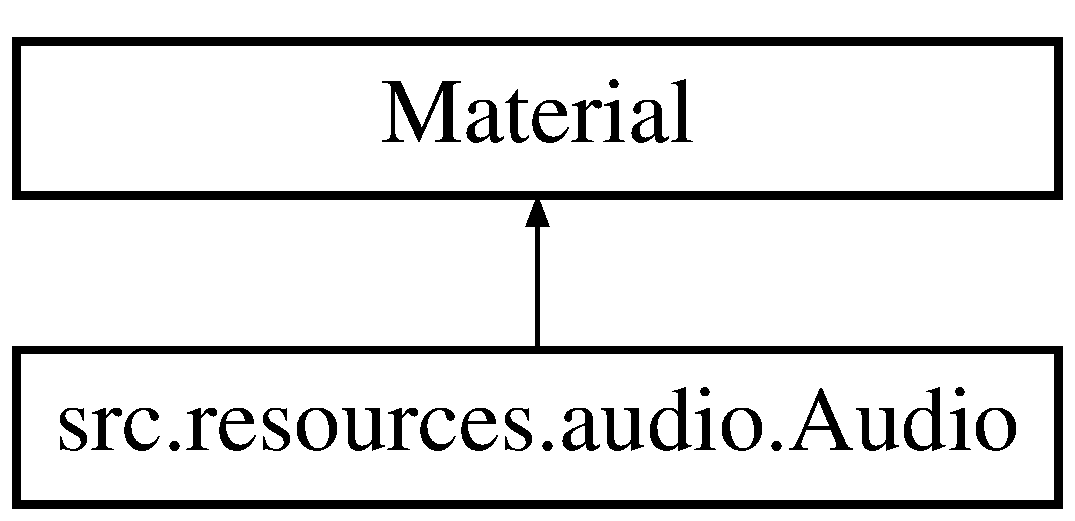
\includegraphics[height=2.000000cm]{classsrc_1_1resources_1_1audio_1_1_audio}
\end{center}
\end{figure}
\subsection*{Public Member Functions}
\begin{DoxyCompactItemize}
\item 
def \hyperlink{classsrc_1_1resources_1_1audio_1_1_audio_af81ebf2e8ce309279b44a7aba68563e9}{\+\_\+\+\_\+init\+\_\+\+\_\+}
\end{DoxyCompactItemize}
\subsection*{Public Attributes}
\begin{DoxyCompactItemize}
\item 
\hyperlink{classsrc_1_1resources_1_1audio_1_1_audio_a8ec1034a29b3c55692fae3be07f54605}{quality}
\item 
\hyperlink{classsrc_1_1resources_1_1audio_1_1_audio_a549dd2605f3d2d09ca8a8618ddf34fc9}{sound}
\item 
\hyperlink{classsrc_1_1resources_1_1audio_1_1_audio_a8d782bb99c64c395286d7f71a8c2ebf8}{start\+Position}
\item 
\hyperlink{classsrc_1_1resources_1_1audio_1_1_audio_a0d0e84fdb0fd8961b8c033dc8d9782ac}{duration\+Of\+Effective\+Speech}
\item 
\hyperlink{classsrc_1_1resources_1_1audio_1_1_audio_ac1da212e2eea3e4fa6ddb5f48c7364c2}{external\+Reference}
\item 
\hyperlink{classsrc_1_1resources_1_1audio_1_1_audio_aadc41b28801de70ba866a40892dce32c}{audio\+File\+Format}
\item 
\hyperlink{classsrc_1_1resources_1_1audio_1_1_audio_aef44fd13d82cd3f79150c76b9b6f4c3e}{transcription}
\end{DoxyCompactItemize}


\subsection{Detailed Description}


Definition at line 5 of file audio.\+py.



\subsection{Constructor \& Destructor Documentation}
\hypertarget{classsrc_1_1resources_1_1audio_1_1_audio_af81ebf2e8ce309279b44a7aba68563e9}{\index{src\+::resources\+::audio\+::\+Audio@{src\+::resources\+::audio\+::\+Audio}!\+\_\+\+\_\+init\+\_\+\+\_\+@{\+\_\+\+\_\+init\+\_\+\+\_\+}}
\index{\+\_\+\+\_\+init\+\_\+\+\_\+@{\+\_\+\+\_\+init\+\_\+\+\_\+}!src\+::resources\+::audio\+::\+Audio@{src\+::resources\+::audio\+::\+Audio}}
\subsubsection[{\+\_\+\+\_\+init\+\_\+\+\_\+}]{\setlength{\rightskip}{0pt plus 5cm}def src.\+resources.\+audio.\+Audio.\+\_\+\+\_\+init\+\_\+\+\_\+ (
\begin{DoxyParamCaption}
\item[{}]{self}
\end{DoxyParamCaption}
)}}\label{classsrc_1_1resources_1_1audio_1_1_audio_af81ebf2e8ce309279b44a7aba68563e9}


Definition at line 6 of file audio.\+py.



\subsection{Member Data Documentation}
\hypertarget{classsrc_1_1resources_1_1audio_1_1_audio_aadc41b28801de70ba866a40892dce32c}{\index{src\+::resources\+::audio\+::\+Audio@{src\+::resources\+::audio\+::\+Audio}!audio\+File\+Format@{audio\+File\+Format}}
\index{audio\+File\+Format@{audio\+File\+Format}!src\+::resources\+::audio\+::\+Audio@{src\+::resources\+::audio\+::\+Audio}}
\subsubsection[{audio\+File\+Format}]{\setlength{\rightskip}{0pt plus 5cm}src.\+resources.\+audio.\+Audio.\+audio\+File\+Format}}\label{classsrc_1_1resources_1_1audio_1_1_audio_aadc41b28801de70ba866a40892dce32c}


Definition at line 12 of file audio.\+py.

\hypertarget{classsrc_1_1resources_1_1audio_1_1_audio_a0d0e84fdb0fd8961b8c033dc8d9782ac}{\index{src\+::resources\+::audio\+::\+Audio@{src\+::resources\+::audio\+::\+Audio}!duration\+Of\+Effective\+Speech@{duration\+Of\+Effective\+Speech}}
\index{duration\+Of\+Effective\+Speech@{duration\+Of\+Effective\+Speech}!src\+::resources\+::audio\+::\+Audio@{src\+::resources\+::audio\+::\+Audio}}
\subsubsection[{duration\+Of\+Effective\+Speech}]{\setlength{\rightskip}{0pt plus 5cm}src.\+resources.\+audio.\+Audio.\+duration\+Of\+Effective\+Speech}}\label{classsrc_1_1resources_1_1audio_1_1_audio_a0d0e84fdb0fd8961b8c033dc8d9782ac}


Definition at line 10 of file audio.\+py.

\hypertarget{classsrc_1_1resources_1_1audio_1_1_audio_ac1da212e2eea3e4fa6ddb5f48c7364c2}{\index{src\+::resources\+::audio\+::\+Audio@{src\+::resources\+::audio\+::\+Audio}!external\+Reference@{external\+Reference}}
\index{external\+Reference@{external\+Reference}!src\+::resources\+::audio\+::\+Audio@{src\+::resources\+::audio\+::\+Audio}}
\subsubsection[{external\+Reference}]{\setlength{\rightskip}{0pt plus 5cm}src.\+resources.\+audio.\+Audio.\+external\+Reference}}\label{classsrc_1_1resources_1_1audio_1_1_audio_ac1da212e2eea3e4fa6ddb5f48c7364c2}


Definition at line 11 of file audio.\+py.

\hypertarget{classsrc_1_1resources_1_1audio_1_1_audio_a8ec1034a29b3c55692fae3be07f54605}{\index{src\+::resources\+::audio\+::\+Audio@{src\+::resources\+::audio\+::\+Audio}!quality@{quality}}
\index{quality@{quality}!src\+::resources\+::audio\+::\+Audio@{src\+::resources\+::audio\+::\+Audio}}
\subsubsection[{quality}]{\setlength{\rightskip}{0pt plus 5cm}src.\+resources.\+audio.\+Audio.\+quality}}\label{classsrc_1_1resources_1_1audio_1_1_audio_a8ec1034a29b3c55692fae3be07f54605}


Definition at line 7 of file audio.\+py.

\hypertarget{classsrc_1_1resources_1_1audio_1_1_audio_a549dd2605f3d2d09ca8a8618ddf34fc9}{\index{src\+::resources\+::audio\+::\+Audio@{src\+::resources\+::audio\+::\+Audio}!sound@{sound}}
\index{sound@{sound}!src\+::resources\+::audio\+::\+Audio@{src\+::resources\+::audio\+::\+Audio}}
\subsubsection[{sound}]{\setlength{\rightskip}{0pt plus 5cm}src.\+resources.\+audio.\+Audio.\+sound}}\label{classsrc_1_1resources_1_1audio_1_1_audio_a549dd2605f3d2d09ca8a8618ddf34fc9}


Definition at line 8 of file audio.\+py.

\hypertarget{classsrc_1_1resources_1_1audio_1_1_audio_a8d782bb99c64c395286d7f71a8c2ebf8}{\index{src\+::resources\+::audio\+::\+Audio@{src\+::resources\+::audio\+::\+Audio}!start\+Position@{start\+Position}}
\index{start\+Position@{start\+Position}!src\+::resources\+::audio\+::\+Audio@{src\+::resources\+::audio\+::\+Audio}}
\subsubsection[{start\+Position}]{\setlength{\rightskip}{0pt plus 5cm}src.\+resources.\+audio.\+Audio.\+start\+Position}}\label{classsrc_1_1resources_1_1audio_1_1_audio_a8d782bb99c64c395286d7f71a8c2ebf8}


Definition at line 9 of file audio.\+py.

\hypertarget{classsrc_1_1resources_1_1audio_1_1_audio_aef44fd13d82cd3f79150c76b9b6f4c3e}{\index{src\+::resources\+::audio\+::\+Audio@{src\+::resources\+::audio\+::\+Audio}!transcription@{transcription}}
\index{transcription@{transcription}!src\+::resources\+::audio\+::\+Audio@{src\+::resources\+::audio\+::\+Audio}}
\subsubsection[{transcription}]{\setlength{\rightskip}{0pt plus 5cm}src.\+resources.\+audio.\+Audio.\+transcription}}\label{classsrc_1_1resources_1_1audio_1_1_audio_aef44fd13d82cd3f79150c76b9b6f4c3e}


Definition at line 13 of file audio.\+py.



The documentation for this class was generated from the following file\+:\begin{DoxyCompactItemize}
\item 
/\+Users/celine/\+Work/\+C\+N\+R\+S/workspace/\+Himal\+Co/dev/lib/lmf/src/resources/\hyperlink{audio_8py}{audio.\+py}\end{DoxyCompactItemize}

\hypertarget{classsrc_1_1morphology_1_1component_1_1_component}{\section{src.\+morphology.\+component.\+Component Class Reference}
\label{classsrc_1_1morphology_1_1component_1_1_component}\index{src.\+morphology.\+component.\+Component@{src.\+morphology.\+component.\+Component}}
}
\subsection*{Public Member Functions}
\begin{DoxyCompactItemize}
\item 
def \hyperlink{classsrc_1_1morphology_1_1component_1_1_component_a3ed51d589f00e3c5c1e9bd64721fed50}{\+\_\+\+\_\+init\+\_\+\+\_\+}
\end{DoxyCompactItemize}
\subsection*{Public Attributes}
\begin{DoxyCompactItemize}
\item 
\hyperlink{classsrc_1_1morphology_1_1component_1_1_component_ab5cb7e1497254923c3298a569001092f}{position}
\end{DoxyCompactItemize}


\subsection{Detailed Description}


Definition at line 3 of file component.\+py.



\subsection{Constructor \& Destructor Documentation}
\hypertarget{classsrc_1_1morphology_1_1component_1_1_component_a3ed51d589f00e3c5c1e9bd64721fed50}{\index{src\+::morphology\+::component\+::\+Component@{src\+::morphology\+::component\+::\+Component}!\+\_\+\+\_\+init\+\_\+\+\_\+@{\+\_\+\+\_\+init\+\_\+\+\_\+}}
\index{\+\_\+\+\_\+init\+\_\+\+\_\+@{\+\_\+\+\_\+init\+\_\+\+\_\+}!src\+::morphology\+::component\+::\+Component@{src\+::morphology\+::component\+::\+Component}}
\subsubsection[{\+\_\+\+\_\+init\+\_\+\+\_\+}]{\setlength{\rightskip}{0pt plus 5cm}def src.\+morphology.\+component.\+Component.\+\_\+\+\_\+init\+\_\+\+\_\+ (
\begin{DoxyParamCaption}
\item[{}]{self}
\end{DoxyParamCaption}
)}}\label{classsrc_1_1morphology_1_1component_1_1_component_a3ed51d589f00e3c5c1e9bd64721fed50}


Definition at line 4 of file component.\+py.



\subsection{Member Data Documentation}
\hypertarget{classsrc_1_1morphology_1_1component_1_1_component_ab5cb7e1497254923c3298a569001092f}{\index{src\+::morphology\+::component\+::\+Component@{src\+::morphology\+::component\+::\+Component}!position@{position}}
\index{position@{position}!src\+::morphology\+::component\+::\+Component@{src\+::morphology\+::component\+::\+Component}}
\subsubsection[{position}]{\setlength{\rightskip}{0pt plus 5cm}src.\+morphology.\+component.\+Component.\+position}}\label{classsrc_1_1morphology_1_1component_1_1_component_ab5cb7e1497254923c3298a569001092f}


Definition at line 5 of file component.\+py.



The documentation for this class was generated from the following file\+:\begin{DoxyCompactItemize}
\item 
/\+Users/celine/\+Work/\+C\+N\+R\+S/workspace/\+Himal\+Co/dev/lib/lmf/src/morphology/\hyperlink{component_8py}{component.\+py}\end{DoxyCompactItemize}

\hypertarget{classsrc_1_1mrd_1_1context_1_1_context}{\section{src.\+mrd.\+context.\+Context Class Reference}
\label{classsrc_1_1mrd_1_1context_1_1_context}\index{src.\+mrd.\+context.\+Context@{src.\+mrd.\+context.\+Context}}
}
\subsection*{Public Member Functions}
\begin{DoxyCompactItemize}
\item 
def \hyperlink{classsrc_1_1mrd_1_1context_1_1_context_a42d39e1c94298a3016de8d32c0c87080}{\+\_\+\+\_\+init\+\_\+\+\_\+}
\end{DoxyCompactItemize}
\subsection*{Public Attributes}
\begin{DoxyCompactItemize}
\item 
\hyperlink{classsrc_1_1mrd_1_1context_1_1_context_ad504d055fa60193f73138b5fbd5a1bf2}{language}
\item 
\hyperlink{classsrc_1_1mrd_1_1context_1_1_context_aa58d522c3916eb637d7a3e8080dccdb3}{type}
\end{DoxyCompactItemize}


\subsection{Detailed Description}


Definition at line 3 of file context.\+py.



\subsection{Constructor \& Destructor Documentation}
\hypertarget{classsrc_1_1mrd_1_1context_1_1_context_a42d39e1c94298a3016de8d32c0c87080}{\index{src\+::mrd\+::context\+::\+Context@{src\+::mrd\+::context\+::\+Context}!\+\_\+\+\_\+init\+\_\+\+\_\+@{\+\_\+\+\_\+init\+\_\+\+\_\+}}
\index{\+\_\+\+\_\+init\+\_\+\+\_\+@{\+\_\+\+\_\+init\+\_\+\+\_\+}!src\+::mrd\+::context\+::\+Context@{src\+::mrd\+::context\+::\+Context}}
\subsubsection[{\+\_\+\+\_\+init\+\_\+\+\_\+}]{\setlength{\rightskip}{0pt plus 5cm}def src.\+mrd.\+context.\+Context.\+\_\+\+\_\+init\+\_\+\+\_\+ (
\begin{DoxyParamCaption}
\item[{}]{self}
\end{DoxyParamCaption}
)}}\label{classsrc_1_1mrd_1_1context_1_1_context_a42d39e1c94298a3016de8d32c0c87080}


Definition at line 4 of file context.\+py.



\subsection{Member Data Documentation}
\hypertarget{classsrc_1_1mrd_1_1context_1_1_context_ad504d055fa60193f73138b5fbd5a1bf2}{\index{src\+::mrd\+::context\+::\+Context@{src\+::mrd\+::context\+::\+Context}!language@{language}}
\index{language@{language}!src\+::mrd\+::context\+::\+Context@{src\+::mrd\+::context\+::\+Context}}
\subsubsection[{language}]{\setlength{\rightskip}{0pt plus 5cm}src.\+mrd.\+context.\+Context.\+language}}\label{classsrc_1_1mrd_1_1context_1_1_context_ad504d055fa60193f73138b5fbd5a1bf2}


Definition at line 5 of file context.\+py.

\hypertarget{classsrc_1_1mrd_1_1context_1_1_context_aa58d522c3916eb637d7a3e8080dccdb3}{\index{src\+::mrd\+::context\+::\+Context@{src\+::mrd\+::context\+::\+Context}!type@{type}}
\index{type@{type}!src\+::mrd\+::context\+::\+Context@{src\+::mrd\+::context\+::\+Context}}
\subsubsection[{type}]{\setlength{\rightskip}{0pt plus 5cm}src.\+mrd.\+context.\+Context.\+type}}\label{classsrc_1_1mrd_1_1context_1_1_context_aa58d522c3916eb637d7a3e8080dccdb3}


Definition at line 6 of file context.\+py.



The documentation for this class was generated from the following file\+:\begin{DoxyCompactItemize}
\item 
/\+Users/celine/\+Work/\+C\+N\+R\+S/workspace/\+Himal\+Co/dev/lib/lmf/src/mrd/\hyperlink{context_8py}{context.\+py}\end{DoxyCompactItemize}

\hypertarget{classsrc_1_1core_1_1definition_1_1_definition}{\section{src.\+core.\+definition.\+Definition Class Reference}
\label{classsrc_1_1core_1_1definition_1_1_definition}\index{src.\+core.\+definition.\+Definition@{src.\+core.\+definition.\+Definition}}
}
\subsection*{Public Member Functions}
\begin{DoxyCompactItemize}
\item 
def \hyperlink{classsrc_1_1core_1_1definition_1_1_definition_ac40b223a739535bd4141937ab01783e7}{\+\_\+\+\_\+init\+\_\+\+\_\+}
\end{DoxyCompactItemize}
\subsection*{Public Attributes}
\begin{DoxyCompactItemize}
\item 
\hyperlink{classsrc_1_1core_1_1definition_1_1_definition_a334db4f6dddebc769ed5c7b44d2f96bf}{language}
\item 
\hyperlink{classsrc_1_1core_1_1definition_1_1_definition_aa135ea494fc7cef95ce3807f979621bf}{definition}
\item 
\hyperlink{classsrc_1_1core_1_1definition_1_1_definition_abcb3ba5e519cc0e98f149754b5810301}{gloss}
\item 
\hyperlink{classsrc_1_1core_1_1definition_1_1_definition_a568bed4ba9074aeb669875ac640b129e}{literally}
\end{DoxyCompactItemize}


\subsection{Detailed Description}


Definition at line 3 of file definition.\+py.



\subsection{Constructor \& Destructor Documentation}
\hypertarget{classsrc_1_1core_1_1definition_1_1_definition_ac40b223a739535bd4141937ab01783e7}{\index{src\+::core\+::definition\+::\+Definition@{src\+::core\+::definition\+::\+Definition}!\+\_\+\+\_\+init\+\_\+\+\_\+@{\+\_\+\+\_\+init\+\_\+\+\_\+}}
\index{\+\_\+\+\_\+init\+\_\+\+\_\+@{\+\_\+\+\_\+init\+\_\+\+\_\+}!src\+::core\+::definition\+::\+Definition@{src\+::core\+::definition\+::\+Definition}}
\subsubsection[{\+\_\+\+\_\+init\+\_\+\+\_\+}]{\setlength{\rightskip}{0pt plus 5cm}def src.\+core.\+definition.\+Definition.\+\_\+\+\_\+init\+\_\+\+\_\+ (
\begin{DoxyParamCaption}
\item[{}]{self}
\end{DoxyParamCaption}
)}}\label{classsrc_1_1core_1_1definition_1_1_definition_ac40b223a739535bd4141937ab01783e7}


Definition at line 4 of file definition.\+py.



\subsection{Member Data Documentation}
\hypertarget{classsrc_1_1core_1_1definition_1_1_definition_aa135ea494fc7cef95ce3807f979621bf}{\index{src\+::core\+::definition\+::\+Definition@{src\+::core\+::definition\+::\+Definition}!definition@{definition}}
\index{definition@{definition}!src\+::core\+::definition\+::\+Definition@{src\+::core\+::definition\+::\+Definition}}
\subsubsection[{definition}]{\setlength{\rightskip}{0pt plus 5cm}src.\+core.\+definition.\+Definition.\+definition}}\label{classsrc_1_1core_1_1definition_1_1_definition_aa135ea494fc7cef95ce3807f979621bf}


Definition at line 6 of file definition.\+py.

\hypertarget{classsrc_1_1core_1_1definition_1_1_definition_abcb3ba5e519cc0e98f149754b5810301}{\index{src\+::core\+::definition\+::\+Definition@{src\+::core\+::definition\+::\+Definition}!gloss@{gloss}}
\index{gloss@{gloss}!src\+::core\+::definition\+::\+Definition@{src\+::core\+::definition\+::\+Definition}}
\subsubsection[{gloss}]{\setlength{\rightskip}{0pt plus 5cm}src.\+core.\+definition.\+Definition.\+gloss}}\label{classsrc_1_1core_1_1definition_1_1_definition_abcb3ba5e519cc0e98f149754b5810301}


Definition at line 7 of file definition.\+py.

\hypertarget{classsrc_1_1core_1_1definition_1_1_definition_a334db4f6dddebc769ed5c7b44d2f96bf}{\index{src\+::core\+::definition\+::\+Definition@{src\+::core\+::definition\+::\+Definition}!language@{language}}
\index{language@{language}!src\+::core\+::definition\+::\+Definition@{src\+::core\+::definition\+::\+Definition}}
\subsubsection[{language}]{\setlength{\rightskip}{0pt plus 5cm}src.\+core.\+definition.\+Definition.\+language}}\label{classsrc_1_1core_1_1definition_1_1_definition_a334db4f6dddebc769ed5c7b44d2f96bf}


Definition at line 5 of file definition.\+py.

\hypertarget{classsrc_1_1core_1_1definition_1_1_definition_a568bed4ba9074aeb669875ac640b129e}{\index{src\+::core\+::definition\+::\+Definition@{src\+::core\+::definition\+::\+Definition}!literally@{literally}}
\index{literally@{literally}!src\+::core\+::definition\+::\+Definition@{src\+::core\+::definition\+::\+Definition}}
\subsubsection[{literally}]{\setlength{\rightskip}{0pt plus 5cm}src.\+core.\+definition.\+Definition.\+literally}}\label{classsrc_1_1core_1_1definition_1_1_definition_a568bed4ba9074aeb669875ac640b129e}


Definition at line 8 of file definition.\+py.



The documentation for this class was generated from the following file\+:\begin{DoxyCompactItemize}
\item 
/\+Users/celine/\+Work/\+C\+N\+R\+S/workspace/\+Himal\+Co/dev/lib/lmf/src/core/\hyperlink{definition_8py}{definition.\+py}\end{DoxyCompactItemize}

\hypertarget{classsrc_1_1mrd_1_1equivalent_1_1_equivalent}{\section{src.\+mrd.\+equivalent.\+Equivalent Class Reference}
\label{classsrc_1_1mrd_1_1equivalent_1_1_equivalent}\index{src.\+mrd.\+equivalent.\+Equivalent@{src.\+mrd.\+equivalent.\+Equivalent}}
}
\subsection*{Public Member Functions}
\begin{DoxyCompactItemize}
\item 
def \hyperlink{classsrc_1_1mrd_1_1equivalent_1_1_equivalent_a83ca8d23dc75be6f6a7e6a318a91aa48}{\+\_\+\+\_\+init\+\_\+\+\_\+}
\end{DoxyCompactItemize}
\subsection*{Public Attributes}
\begin{DoxyCompactItemize}
\item 
\hyperlink{classsrc_1_1mrd_1_1equivalent_1_1_equivalent_a827bb0b73adca115ffdf6f5a95f807bf}{language}
\item 
\hyperlink{classsrc_1_1mrd_1_1equivalent_1_1_equivalent_a607911fadc9f5751ca553cb7c47d300f}{translation}
\end{DoxyCompactItemize}


\subsection{Detailed Description}


Definition at line 3 of file equivalent.\+py.



\subsection{Constructor \& Destructor Documentation}
\hypertarget{classsrc_1_1mrd_1_1equivalent_1_1_equivalent_a83ca8d23dc75be6f6a7e6a318a91aa48}{\index{src\+::mrd\+::equivalent\+::\+Equivalent@{src\+::mrd\+::equivalent\+::\+Equivalent}!\+\_\+\+\_\+init\+\_\+\+\_\+@{\+\_\+\+\_\+init\+\_\+\+\_\+}}
\index{\+\_\+\+\_\+init\+\_\+\+\_\+@{\+\_\+\+\_\+init\+\_\+\+\_\+}!src\+::mrd\+::equivalent\+::\+Equivalent@{src\+::mrd\+::equivalent\+::\+Equivalent}}
\subsubsection[{\+\_\+\+\_\+init\+\_\+\+\_\+}]{\setlength{\rightskip}{0pt plus 5cm}def src.\+mrd.\+equivalent.\+Equivalent.\+\_\+\+\_\+init\+\_\+\+\_\+ (
\begin{DoxyParamCaption}
\item[{}]{self}
\end{DoxyParamCaption}
)}}\label{classsrc_1_1mrd_1_1equivalent_1_1_equivalent_a83ca8d23dc75be6f6a7e6a318a91aa48}


Definition at line 4 of file equivalent.\+py.



\subsection{Member Data Documentation}
\hypertarget{classsrc_1_1mrd_1_1equivalent_1_1_equivalent_a827bb0b73adca115ffdf6f5a95f807bf}{\index{src\+::mrd\+::equivalent\+::\+Equivalent@{src\+::mrd\+::equivalent\+::\+Equivalent}!language@{language}}
\index{language@{language}!src\+::mrd\+::equivalent\+::\+Equivalent@{src\+::mrd\+::equivalent\+::\+Equivalent}}
\subsubsection[{language}]{\setlength{\rightskip}{0pt plus 5cm}src.\+mrd.\+equivalent.\+Equivalent.\+language}}\label{classsrc_1_1mrd_1_1equivalent_1_1_equivalent_a827bb0b73adca115ffdf6f5a95f807bf}


Definition at line 5 of file equivalent.\+py.

\hypertarget{classsrc_1_1mrd_1_1equivalent_1_1_equivalent_a607911fadc9f5751ca553cb7c47d300f}{\index{src\+::mrd\+::equivalent\+::\+Equivalent@{src\+::mrd\+::equivalent\+::\+Equivalent}!translation@{translation}}
\index{translation@{translation}!src\+::mrd\+::equivalent\+::\+Equivalent@{src\+::mrd\+::equivalent\+::\+Equivalent}}
\subsubsection[{translation}]{\setlength{\rightskip}{0pt plus 5cm}src.\+mrd.\+equivalent.\+Equivalent.\+translation}}\label{classsrc_1_1mrd_1_1equivalent_1_1_equivalent_a607911fadc9f5751ca553cb7c47d300f}


Definition at line 6 of file equivalent.\+py.



The documentation for this class was generated from the following file\+:\begin{DoxyCompactItemize}
\item 
/\+Users/celine/\+Work/\+C\+N\+R\+S/workspace/\+Himal\+Co/dev/lib/lmf/src/mrd/\hyperlink{equivalent_8py}{equivalent.\+py}\end{DoxyCompactItemize}

\hypertarget{classsrc_1_1utils_1_1error__handling_1_1_error_handling}{\section{src.\+utils.\+error\+\_\+handling.\+Error\+Handling Class Reference}
\label{classsrc_1_1utils_1_1error__handling_1_1_error_handling}\index{src.\+utils.\+error\+\_\+handling.\+Error\+Handling@{src.\+utils.\+error\+\_\+handling.\+Error\+Handling}}
}
\subsection*{Public Member Functions}
\begin{DoxyCompactItemize}
\item 
def \hyperlink{classsrc_1_1utils_1_1error__handling_1_1_error_handling_a075a85ea959939e8063dcde9cc93c10f}{\+\_\+\+\_\+init\+\_\+\+\_\+}
\end{DoxyCompactItemize}


\subsection{Detailed Description}


Definition at line 3 of file error\+\_\+handling.\+py.



\subsection{Constructor \& Destructor Documentation}
\hypertarget{classsrc_1_1utils_1_1error__handling_1_1_error_handling_a075a85ea959939e8063dcde9cc93c10f}{\index{src\+::utils\+::error\+\_\+handling\+::\+Error\+Handling@{src\+::utils\+::error\+\_\+handling\+::\+Error\+Handling}!\+\_\+\+\_\+init\+\_\+\+\_\+@{\+\_\+\+\_\+init\+\_\+\+\_\+}}
\index{\+\_\+\+\_\+init\+\_\+\+\_\+@{\+\_\+\+\_\+init\+\_\+\+\_\+}!src\+::utils\+::error\+\_\+handling\+::\+Error\+Handling@{src\+::utils\+::error\+\_\+handling\+::\+Error\+Handling}}
\subsubsection[{\+\_\+\+\_\+init\+\_\+\+\_\+}]{\setlength{\rightskip}{0pt plus 5cm}def src.\+utils.\+error\+\_\+handling.\+Error\+Handling.\+\_\+\+\_\+init\+\_\+\+\_\+ (
\begin{DoxyParamCaption}
\item[{}]{self}
\end{DoxyParamCaption}
)}}\label{classsrc_1_1utils_1_1error__handling_1_1_error_handling_a075a85ea959939e8063dcde9cc93c10f}


Definition at line 4 of file error\+\_\+handling.\+py.



The documentation for this class was generated from the following file\+:\begin{DoxyCompactItemize}
\item 
/\+Users/celine/\+Work/\+C\+N\+R\+S/workspace/\+Himal\+Co/dev/lib/lmf/src/utils/\hyperlink{error__handling_8py}{error\+\_\+handling.\+py}\end{DoxyCompactItemize}

\hypertarget{classsrc_1_1core_1_1form_1_1_form}{\section{src.\+core.\+form.\+Form Class Reference}
\label{classsrc_1_1core_1_1form_1_1_form}\index{src.\+core.\+form.\+Form@{src.\+core.\+form.\+Form}}
}
\subsection*{Public Member Functions}
\begin{DoxyCompactItemize}
\item 
def \hyperlink{classsrc_1_1core_1_1form_1_1_form_ad690f26f41ad66656c19e30ed1d7827d}{\+\_\+\+\_\+init\+\_\+\+\_\+}
\end{DoxyCompactItemize}
\subsection*{Public Attributes}
\begin{DoxyCompactItemize}
\item 
\hyperlink{classsrc_1_1core_1_1form_1_1_form_a0e200dbcf3f01a53844854ae84509c15}{variant\+Form}
\item 
\hyperlink{classsrc_1_1core_1_1form_1_1_form_afc077dc1d02f87ed61603f0ddeaebde8}{type}
\end{DoxyCompactItemize}


\subsection{Detailed Description}


Definition at line 3 of file form.\+py.



\subsection{Constructor \& Destructor Documentation}
\hypertarget{classsrc_1_1core_1_1form_1_1_form_ad690f26f41ad66656c19e30ed1d7827d}{\index{src\+::core\+::form\+::\+Form@{src\+::core\+::form\+::\+Form}!\+\_\+\+\_\+init\+\_\+\+\_\+@{\+\_\+\+\_\+init\+\_\+\+\_\+}}
\index{\+\_\+\+\_\+init\+\_\+\+\_\+@{\+\_\+\+\_\+init\+\_\+\+\_\+}!src\+::core\+::form\+::\+Form@{src\+::core\+::form\+::\+Form}}
\subsubsection[{\+\_\+\+\_\+init\+\_\+\+\_\+}]{\setlength{\rightskip}{0pt plus 5cm}def src.\+core.\+form.\+Form.\+\_\+\+\_\+init\+\_\+\+\_\+ (
\begin{DoxyParamCaption}
\item[{}]{self}
\end{DoxyParamCaption}
)}}\label{classsrc_1_1core_1_1form_1_1_form_ad690f26f41ad66656c19e30ed1d7827d}


Definition at line 4 of file form.\+py.



\subsection{Member Data Documentation}
\hypertarget{classsrc_1_1core_1_1form_1_1_form_afc077dc1d02f87ed61603f0ddeaebde8}{\index{src\+::core\+::form\+::\+Form@{src\+::core\+::form\+::\+Form}!type@{type}}
\index{type@{type}!src\+::core\+::form\+::\+Form@{src\+::core\+::form\+::\+Form}}
\subsubsection[{type}]{\setlength{\rightskip}{0pt plus 5cm}src.\+core.\+form.\+Form.\+type}}\label{classsrc_1_1core_1_1form_1_1_form_afc077dc1d02f87ed61603f0ddeaebde8}


Definition at line 6 of file form.\+py.

\hypertarget{classsrc_1_1core_1_1form_1_1_form_a0e200dbcf3f01a53844854ae84509c15}{\index{src\+::core\+::form\+::\+Form@{src\+::core\+::form\+::\+Form}!variant\+Form@{variant\+Form}}
\index{variant\+Form@{variant\+Form}!src\+::core\+::form\+::\+Form@{src\+::core\+::form\+::\+Form}}
\subsubsection[{variant\+Form}]{\setlength{\rightskip}{0pt plus 5cm}src.\+core.\+form.\+Form.\+variant\+Form}}\label{classsrc_1_1core_1_1form_1_1_form_a0e200dbcf3f01a53844854ae84509c15}


Definition at line 5 of file form.\+py.



The documentation for this class was generated from the following file\+:\begin{DoxyCompactItemize}
\item 
/\+Users/celine/\+Work/\+C\+N\+R\+S/workspace/\+Himal\+Co/dev/lib/lmf/src/core/\hyperlink{form_8py}{form.\+py}\end{DoxyCompactItemize}

\hypertarget{classsrc_1_1core_1_1form__representation_1_1_form_representation}{\section{src.\+core.\+form\+\_\+representation.\+Form\+Representation Class Reference}
\label{classsrc_1_1core_1_1form__representation_1_1_form_representation}\index{src.\+core.\+form\+\_\+representation.\+Form\+Representation@{src.\+core.\+form\+\_\+representation.\+Form\+Representation}}
}
Inheritance diagram for src.\+core.\+form\+\_\+representation.\+Form\+Representation\+:\begin{figure}[H]
\begin{center}
\leavevmode
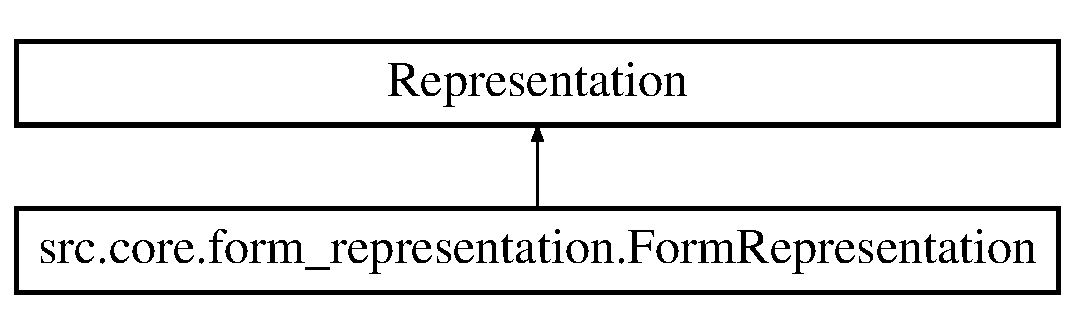
\includegraphics[height=2.000000cm]{classsrc_1_1core_1_1form__representation_1_1_form_representation}
\end{center}
\end{figure}
\subsection*{Public Member Functions}
\begin{DoxyCompactItemize}
\item 
def \hyperlink{classsrc_1_1core_1_1form__representation_1_1_form_representation_a1ee2134537d3b54509f31ddd9fa21ead}{\+\_\+\+\_\+init\+\_\+\+\_\+}
\end{DoxyCompactItemize}
\subsection*{Public Attributes}
\begin{DoxyCompactItemize}
\item 
\hyperlink{classsrc_1_1core_1_1form__representation_1_1_form_representation_afe034e736b48176000fca76d8b8604ef}{transliteration}
\item 
\hyperlink{classsrc_1_1core_1_1form__representation_1_1_form_representation_a5b9d85ec2c63d3d93f09da2c569234a0}{tone}
\item 
\hyperlink{classsrc_1_1core_1_1form__representation_1_1_form_representation_a810f62688bdea5e822712c4382c6d6f3}{geographical\+Variant}
\item 
\hyperlink{classsrc_1_1core_1_1form__representation_1_1_form_representation_aab45e1639b37a2b07631aa47729ed09d}{phonetic\+Form}
\item 
\hyperlink{classsrc_1_1core_1_1form__representation_1_1_form_representation_ab29cfe204850c7d0d7348605b570cc5c}{contextual\+Variation}
\item 
\hyperlink{classsrc_1_1core_1_1form__representation_1_1_form_representation_acbb491e2075ba5ce28b7159e1fa42154}{spelling\+Variant}
\item 
\hyperlink{classsrc_1_1core_1_1form__representation_1_1_form_representation_a467fc5cd662d8577f16725637a7dc7ad}{citation\+Form}
\item 
\hyperlink{classsrc_1_1core_1_1form__representation_1_1_form_representation_abc0dcbe740b5309dd4e4a111bdc11965}{dialect}
\item 
\hyperlink{classsrc_1_1core_1_1form__representation_1_1_form_representation_afd3e6d24af2c00ddf6286305aea9bb6f}{language}
\item 
\hyperlink{classsrc_1_1core_1_1form__representation_1_1_form_representation_a4d1bead536706462cc8c8851ffb53ad5}{script\+Name}
\end{DoxyCompactItemize}


\subsection{Detailed Description}


Definition at line 5 of file form\+\_\+representation.\+py.



\subsection{Constructor \& Destructor Documentation}
\hypertarget{classsrc_1_1core_1_1form__representation_1_1_form_representation_a1ee2134537d3b54509f31ddd9fa21ead}{\index{src\+::core\+::form\+\_\+representation\+::\+Form\+Representation@{src\+::core\+::form\+\_\+representation\+::\+Form\+Representation}!\+\_\+\+\_\+init\+\_\+\+\_\+@{\+\_\+\+\_\+init\+\_\+\+\_\+}}
\index{\+\_\+\+\_\+init\+\_\+\+\_\+@{\+\_\+\+\_\+init\+\_\+\+\_\+}!src\+::core\+::form\+\_\+representation\+::\+Form\+Representation@{src\+::core\+::form\+\_\+representation\+::\+Form\+Representation}}
\subsubsection[{\+\_\+\+\_\+init\+\_\+\+\_\+}]{\setlength{\rightskip}{0pt plus 5cm}def src.\+core.\+form\+\_\+representation.\+Form\+Representation.\+\_\+\+\_\+init\+\_\+\+\_\+ (
\begin{DoxyParamCaption}
\item[{}]{self}
\end{DoxyParamCaption}
)}}\label{classsrc_1_1core_1_1form__representation_1_1_form_representation_a1ee2134537d3b54509f31ddd9fa21ead}


Definition at line 6 of file form\+\_\+representation.\+py.



\subsection{Member Data Documentation}
\hypertarget{classsrc_1_1core_1_1form__representation_1_1_form_representation_a467fc5cd662d8577f16725637a7dc7ad}{\index{src\+::core\+::form\+\_\+representation\+::\+Form\+Representation@{src\+::core\+::form\+\_\+representation\+::\+Form\+Representation}!citation\+Form@{citation\+Form}}
\index{citation\+Form@{citation\+Form}!src\+::core\+::form\+\_\+representation\+::\+Form\+Representation@{src\+::core\+::form\+\_\+representation\+::\+Form\+Representation}}
\subsubsection[{citation\+Form}]{\setlength{\rightskip}{0pt plus 5cm}src.\+core.\+form\+\_\+representation.\+Form\+Representation.\+citation\+Form}}\label{classsrc_1_1core_1_1form__representation_1_1_form_representation_a467fc5cd662d8577f16725637a7dc7ad}


Definition at line 13 of file form\+\_\+representation.\+py.

\hypertarget{classsrc_1_1core_1_1form__representation_1_1_form_representation_ab29cfe204850c7d0d7348605b570cc5c}{\index{src\+::core\+::form\+\_\+representation\+::\+Form\+Representation@{src\+::core\+::form\+\_\+representation\+::\+Form\+Representation}!contextual\+Variation@{contextual\+Variation}}
\index{contextual\+Variation@{contextual\+Variation}!src\+::core\+::form\+\_\+representation\+::\+Form\+Representation@{src\+::core\+::form\+\_\+representation\+::\+Form\+Representation}}
\subsubsection[{contextual\+Variation}]{\setlength{\rightskip}{0pt plus 5cm}src.\+core.\+form\+\_\+representation.\+Form\+Representation.\+contextual\+Variation}}\label{classsrc_1_1core_1_1form__representation_1_1_form_representation_ab29cfe204850c7d0d7348605b570cc5c}


Definition at line 11 of file form\+\_\+representation.\+py.

\hypertarget{classsrc_1_1core_1_1form__representation_1_1_form_representation_abc0dcbe740b5309dd4e4a111bdc11965}{\index{src\+::core\+::form\+\_\+representation\+::\+Form\+Representation@{src\+::core\+::form\+\_\+representation\+::\+Form\+Representation}!dialect@{dialect}}
\index{dialect@{dialect}!src\+::core\+::form\+\_\+representation\+::\+Form\+Representation@{src\+::core\+::form\+\_\+representation\+::\+Form\+Representation}}
\subsubsection[{dialect}]{\setlength{\rightskip}{0pt plus 5cm}src.\+core.\+form\+\_\+representation.\+Form\+Representation.\+dialect}}\label{classsrc_1_1core_1_1form__representation_1_1_form_representation_abc0dcbe740b5309dd4e4a111bdc11965}


Definition at line 14 of file form\+\_\+representation.\+py.

\hypertarget{classsrc_1_1core_1_1form__representation_1_1_form_representation_a810f62688bdea5e822712c4382c6d6f3}{\index{src\+::core\+::form\+\_\+representation\+::\+Form\+Representation@{src\+::core\+::form\+\_\+representation\+::\+Form\+Representation}!geographical\+Variant@{geographical\+Variant}}
\index{geographical\+Variant@{geographical\+Variant}!src\+::core\+::form\+\_\+representation\+::\+Form\+Representation@{src\+::core\+::form\+\_\+representation\+::\+Form\+Representation}}
\subsubsection[{geographical\+Variant}]{\setlength{\rightskip}{0pt plus 5cm}src.\+core.\+form\+\_\+representation.\+Form\+Representation.\+geographical\+Variant}}\label{classsrc_1_1core_1_1form__representation_1_1_form_representation_a810f62688bdea5e822712c4382c6d6f3}


Definition at line 9 of file form\+\_\+representation.\+py.

\hypertarget{classsrc_1_1core_1_1form__representation_1_1_form_representation_afd3e6d24af2c00ddf6286305aea9bb6f}{\index{src\+::core\+::form\+\_\+representation\+::\+Form\+Representation@{src\+::core\+::form\+\_\+representation\+::\+Form\+Representation}!language@{language}}
\index{language@{language}!src\+::core\+::form\+\_\+representation\+::\+Form\+Representation@{src\+::core\+::form\+\_\+representation\+::\+Form\+Representation}}
\subsubsection[{language}]{\setlength{\rightskip}{0pt plus 5cm}src.\+core.\+form\+\_\+representation.\+Form\+Representation.\+language}}\label{classsrc_1_1core_1_1form__representation_1_1_form_representation_afd3e6d24af2c00ddf6286305aea9bb6f}


Definition at line 15 of file form\+\_\+representation.\+py.

\hypertarget{classsrc_1_1core_1_1form__representation_1_1_form_representation_aab45e1639b37a2b07631aa47729ed09d}{\index{src\+::core\+::form\+\_\+representation\+::\+Form\+Representation@{src\+::core\+::form\+\_\+representation\+::\+Form\+Representation}!phonetic\+Form@{phonetic\+Form}}
\index{phonetic\+Form@{phonetic\+Form}!src\+::core\+::form\+\_\+representation\+::\+Form\+Representation@{src\+::core\+::form\+\_\+representation\+::\+Form\+Representation}}
\subsubsection[{phonetic\+Form}]{\setlength{\rightskip}{0pt plus 5cm}src.\+core.\+form\+\_\+representation.\+Form\+Representation.\+phonetic\+Form}}\label{classsrc_1_1core_1_1form__representation_1_1_form_representation_aab45e1639b37a2b07631aa47729ed09d}


Definition at line 10 of file form\+\_\+representation.\+py.

\hypertarget{classsrc_1_1core_1_1form__representation_1_1_form_representation_a4d1bead536706462cc8c8851ffb53ad5}{\index{src\+::core\+::form\+\_\+representation\+::\+Form\+Representation@{src\+::core\+::form\+\_\+representation\+::\+Form\+Representation}!script\+Name@{script\+Name}}
\index{script\+Name@{script\+Name}!src\+::core\+::form\+\_\+representation\+::\+Form\+Representation@{src\+::core\+::form\+\_\+representation\+::\+Form\+Representation}}
\subsubsection[{script\+Name}]{\setlength{\rightskip}{0pt plus 5cm}src.\+core.\+form\+\_\+representation.\+Form\+Representation.\+script\+Name}}\label{classsrc_1_1core_1_1form__representation_1_1_form_representation_a4d1bead536706462cc8c8851ffb53ad5}


Definition at line 16 of file form\+\_\+representation.\+py.

\hypertarget{classsrc_1_1core_1_1form__representation_1_1_form_representation_acbb491e2075ba5ce28b7159e1fa42154}{\index{src\+::core\+::form\+\_\+representation\+::\+Form\+Representation@{src\+::core\+::form\+\_\+representation\+::\+Form\+Representation}!spelling\+Variant@{spelling\+Variant}}
\index{spelling\+Variant@{spelling\+Variant}!src\+::core\+::form\+\_\+representation\+::\+Form\+Representation@{src\+::core\+::form\+\_\+representation\+::\+Form\+Representation}}
\subsubsection[{spelling\+Variant}]{\setlength{\rightskip}{0pt plus 5cm}src.\+core.\+form\+\_\+representation.\+Form\+Representation.\+spelling\+Variant}}\label{classsrc_1_1core_1_1form__representation_1_1_form_representation_acbb491e2075ba5ce28b7159e1fa42154}


Definition at line 12 of file form\+\_\+representation.\+py.

\hypertarget{classsrc_1_1core_1_1form__representation_1_1_form_representation_a5b9d85ec2c63d3d93f09da2c569234a0}{\index{src\+::core\+::form\+\_\+representation\+::\+Form\+Representation@{src\+::core\+::form\+\_\+representation\+::\+Form\+Representation}!tone@{tone}}
\index{tone@{tone}!src\+::core\+::form\+\_\+representation\+::\+Form\+Representation@{src\+::core\+::form\+\_\+representation\+::\+Form\+Representation}}
\subsubsection[{tone}]{\setlength{\rightskip}{0pt plus 5cm}src.\+core.\+form\+\_\+representation.\+Form\+Representation.\+tone}}\label{classsrc_1_1core_1_1form__representation_1_1_form_representation_a5b9d85ec2c63d3d93f09da2c569234a0}


Definition at line 8 of file form\+\_\+representation.\+py.

\hypertarget{classsrc_1_1core_1_1form__representation_1_1_form_representation_afe034e736b48176000fca76d8b8604ef}{\index{src\+::core\+::form\+\_\+representation\+::\+Form\+Representation@{src\+::core\+::form\+\_\+representation\+::\+Form\+Representation}!transliteration@{transliteration}}
\index{transliteration@{transliteration}!src\+::core\+::form\+\_\+representation\+::\+Form\+Representation@{src\+::core\+::form\+\_\+representation\+::\+Form\+Representation}}
\subsubsection[{transliteration}]{\setlength{\rightskip}{0pt plus 5cm}src.\+core.\+form\+\_\+representation.\+Form\+Representation.\+transliteration}}\label{classsrc_1_1core_1_1form__representation_1_1_form_representation_afe034e736b48176000fca76d8b8604ef}


Definition at line 7 of file form\+\_\+representation.\+py.



The documentation for this class was generated from the following file\+:\begin{DoxyCompactItemize}
\item 
/\+Users/celine/\+Work/\+C\+N\+R\+S/workspace/\+Himal\+Co/dev/lib/lmf/src/core/\hyperlink{form__representation_8py}{form\+\_\+representation.\+py}\end{DoxyCompactItemize}

\hypertarget{classsrc_1_1core_1_1global__information_1_1_global_information}{\section{src.\+core.\+global\+\_\+information.\+Global\+Information Class Reference}
\label{classsrc_1_1core_1_1global__information_1_1_global_information}\index{src.\+core.\+global\+\_\+information.\+Global\+Information@{src.\+core.\+global\+\_\+information.\+Global\+Information}}
}
\subsection*{Public Member Functions}
\begin{DoxyCompactItemize}
\item 
def \hyperlink{classsrc_1_1core_1_1global__information_1_1_global_information_a6538239b5662f3a2753673c7c219bfe9}{\+\_\+\+\_\+init\+\_\+\+\_\+}
\end{DoxyCompactItemize}
\subsection*{Public Attributes}
\begin{DoxyCompactItemize}
\item 
\hyperlink{classsrc_1_1core_1_1global__information_1_1_global_information_a67df050014c5e4f44cd0d34c5c97da3f}{language\+Code}
\item 
\hyperlink{classsrc_1_1core_1_1global__information_1_1_global_information_a75ba6ca3c99930f8b46906f7622c36aa}{author}
\item 
\hyperlink{classsrc_1_1core_1_1global__information_1_1_global_information_a48a0e9271d030e4d1b1f89aa7f8ecf39}{version}
\item 
\hyperlink{classsrc_1_1core_1_1global__information_1_1_global_information_a4c3c1476f39150406420455273d6dbd0}{last\+Update}
\item 
\hyperlink{classsrc_1_1core_1_1global__information_1_1_global_information_ae9146603dba3654d72081b02e68c99d7}{license}
\item 
\hyperlink{classsrc_1_1core_1_1global__information_1_1_global_information_affc1f1a49521c8d27523b47ccf7a0724}{character\+Encoding}
\item 
\hyperlink{classsrc_1_1core_1_1global__information_1_1_global_information_aaa8008762d8d3afa73ea17c110d3813b}{date\+Coding}
\item 
\hyperlink{classsrc_1_1core_1_1global__information_1_1_global_information_aa6e73ed38a7a4faf7a1d076b03e2afa7}{creation\+Date}
\item 
\hyperlink{classsrc_1_1core_1_1global__information_1_1_global_information_aa75b2e04e65ddb9d9f7f78c15d049961}{project\+Name}
\item 
\hyperlink{classsrc_1_1core_1_1global__information_1_1_global_information_ad9432db5c5b0393589658eb92a17bce3}{description}
\item 
\hyperlink{classsrc_1_1core_1_1global__information_1_1_global_information_a036b2ccf0faed59803b88f4ecb8dfc19}{bibliographic\+Citation}
\end{DoxyCompactItemize}


\subsection{Detailed Description}


Definition at line 3 of file global\+\_\+information.\+py.



\subsection{Constructor \& Destructor Documentation}
\hypertarget{classsrc_1_1core_1_1global__information_1_1_global_information_a6538239b5662f3a2753673c7c219bfe9}{\index{src\+::core\+::global\+\_\+information\+::\+Global\+Information@{src\+::core\+::global\+\_\+information\+::\+Global\+Information}!\+\_\+\+\_\+init\+\_\+\+\_\+@{\+\_\+\+\_\+init\+\_\+\+\_\+}}
\index{\+\_\+\+\_\+init\+\_\+\+\_\+@{\+\_\+\+\_\+init\+\_\+\+\_\+}!src\+::core\+::global\+\_\+information\+::\+Global\+Information@{src\+::core\+::global\+\_\+information\+::\+Global\+Information}}
\subsubsection[{\+\_\+\+\_\+init\+\_\+\+\_\+}]{\setlength{\rightskip}{0pt plus 5cm}def src.\+core.\+global\+\_\+information.\+Global\+Information.\+\_\+\+\_\+init\+\_\+\+\_\+ (
\begin{DoxyParamCaption}
\item[{}]{self}
\end{DoxyParamCaption}
)}}\label{classsrc_1_1core_1_1global__information_1_1_global_information_a6538239b5662f3a2753673c7c219bfe9}


Definition at line 4 of file global\+\_\+information.\+py.



\subsection{Member Data Documentation}
\hypertarget{classsrc_1_1core_1_1global__information_1_1_global_information_a75ba6ca3c99930f8b46906f7622c36aa}{\index{src\+::core\+::global\+\_\+information\+::\+Global\+Information@{src\+::core\+::global\+\_\+information\+::\+Global\+Information}!author@{author}}
\index{author@{author}!src\+::core\+::global\+\_\+information\+::\+Global\+Information@{src\+::core\+::global\+\_\+information\+::\+Global\+Information}}
\subsubsection[{author}]{\setlength{\rightskip}{0pt plus 5cm}src.\+core.\+global\+\_\+information.\+Global\+Information.\+author}}\label{classsrc_1_1core_1_1global__information_1_1_global_information_a75ba6ca3c99930f8b46906f7622c36aa}


Definition at line 6 of file global\+\_\+information.\+py.

\hypertarget{classsrc_1_1core_1_1global__information_1_1_global_information_a036b2ccf0faed59803b88f4ecb8dfc19}{\index{src\+::core\+::global\+\_\+information\+::\+Global\+Information@{src\+::core\+::global\+\_\+information\+::\+Global\+Information}!bibliographic\+Citation@{bibliographic\+Citation}}
\index{bibliographic\+Citation@{bibliographic\+Citation}!src\+::core\+::global\+\_\+information\+::\+Global\+Information@{src\+::core\+::global\+\_\+information\+::\+Global\+Information}}
\subsubsection[{bibliographic\+Citation}]{\setlength{\rightskip}{0pt plus 5cm}src.\+core.\+global\+\_\+information.\+Global\+Information.\+bibliographic\+Citation}}\label{classsrc_1_1core_1_1global__information_1_1_global_information_a036b2ccf0faed59803b88f4ecb8dfc19}


Definition at line 15 of file global\+\_\+information.\+py.

\hypertarget{classsrc_1_1core_1_1global__information_1_1_global_information_affc1f1a49521c8d27523b47ccf7a0724}{\index{src\+::core\+::global\+\_\+information\+::\+Global\+Information@{src\+::core\+::global\+\_\+information\+::\+Global\+Information}!character\+Encoding@{character\+Encoding}}
\index{character\+Encoding@{character\+Encoding}!src\+::core\+::global\+\_\+information\+::\+Global\+Information@{src\+::core\+::global\+\_\+information\+::\+Global\+Information}}
\subsubsection[{character\+Encoding}]{\setlength{\rightskip}{0pt plus 5cm}src.\+core.\+global\+\_\+information.\+Global\+Information.\+character\+Encoding}}\label{classsrc_1_1core_1_1global__information_1_1_global_information_affc1f1a49521c8d27523b47ccf7a0724}


Definition at line 10 of file global\+\_\+information.\+py.

\hypertarget{classsrc_1_1core_1_1global__information_1_1_global_information_aa6e73ed38a7a4faf7a1d076b03e2afa7}{\index{src\+::core\+::global\+\_\+information\+::\+Global\+Information@{src\+::core\+::global\+\_\+information\+::\+Global\+Information}!creation\+Date@{creation\+Date}}
\index{creation\+Date@{creation\+Date}!src\+::core\+::global\+\_\+information\+::\+Global\+Information@{src\+::core\+::global\+\_\+information\+::\+Global\+Information}}
\subsubsection[{creation\+Date}]{\setlength{\rightskip}{0pt plus 5cm}src.\+core.\+global\+\_\+information.\+Global\+Information.\+creation\+Date}}\label{classsrc_1_1core_1_1global__information_1_1_global_information_aa6e73ed38a7a4faf7a1d076b03e2afa7}


Definition at line 12 of file global\+\_\+information.\+py.

\hypertarget{classsrc_1_1core_1_1global__information_1_1_global_information_aaa8008762d8d3afa73ea17c110d3813b}{\index{src\+::core\+::global\+\_\+information\+::\+Global\+Information@{src\+::core\+::global\+\_\+information\+::\+Global\+Information}!date\+Coding@{date\+Coding}}
\index{date\+Coding@{date\+Coding}!src\+::core\+::global\+\_\+information\+::\+Global\+Information@{src\+::core\+::global\+\_\+information\+::\+Global\+Information}}
\subsubsection[{date\+Coding}]{\setlength{\rightskip}{0pt plus 5cm}src.\+core.\+global\+\_\+information.\+Global\+Information.\+date\+Coding}}\label{classsrc_1_1core_1_1global__information_1_1_global_information_aaa8008762d8d3afa73ea17c110d3813b}


Definition at line 11 of file global\+\_\+information.\+py.

\hypertarget{classsrc_1_1core_1_1global__information_1_1_global_information_ad9432db5c5b0393589658eb92a17bce3}{\index{src\+::core\+::global\+\_\+information\+::\+Global\+Information@{src\+::core\+::global\+\_\+information\+::\+Global\+Information}!description@{description}}
\index{description@{description}!src\+::core\+::global\+\_\+information\+::\+Global\+Information@{src\+::core\+::global\+\_\+information\+::\+Global\+Information}}
\subsubsection[{description}]{\setlength{\rightskip}{0pt plus 5cm}src.\+core.\+global\+\_\+information.\+Global\+Information.\+description}}\label{classsrc_1_1core_1_1global__information_1_1_global_information_ad9432db5c5b0393589658eb92a17bce3}


Definition at line 14 of file global\+\_\+information.\+py.

\hypertarget{classsrc_1_1core_1_1global__information_1_1_global_information_a67df050014c5e4f44cd0d34c5c97da3f}{\index{src\+::core\+::global\+\_\+information\+::\+Global\+Information@{src\+::core\+::global\+\_\+information\+::\+Global\+Information}!language\+Code@{language\+Code}}
\index{language\+Code@{language\+Code}!src\+::core\+::global\+\_\+information\+::\+Global\+Information@{src\+::core\+::global\+\_\+information\+::\+Global\+Information}}
\subsubsection[{language\+Code}]{\setlength{\rightskip}{0pt plus 5cm}src.\+core.\+global\+\_\+information.\+Global\+Information.\+language\+Code}}\label{classsrc_1_1core_1_1global__information_1_1_global_information_a67df050014c5e4f44cd0d34c5c97da3f}


Definition at line 5 of file global\+\_\+information.\+py.

\hypertarget{classsrc_1_1core_1_1global__information_1_1_global_information_a4c3c1476f39150406420455273d6dbd0}{\index{src\+::core\+::global\+\_\+information\+::\+Global\+Information@{src\+::core\+::global\+\_\+information\+::\+Global\+Information}!last\+Update@{last\+Update}}
\index{last\+Update@{last\+Update}!src\+::core\+::global\+\_\+information\+::\+Global\+Information@{src\+::core\+::global\+\_\+information\+::\+Global\+Information}}
\subsubsection[{last\+Update}]{\setlength{\rightskip}{0pt plus 5cm}src.\+core.\+global\+\_\+information.\+Global\+Information.\+last\+Update}}\label{classsrc_1_1core_1_1global__information_1_1_global_information_a4c3c1476f39150406420455273d6dbd0}


Definition at line 8 of file global\+\_\+information.\+py.

\hypertarget{classsrc_1_1core_1_1global__information_1_1_global_information_ae9146603dba3654d72081b02e68c99d7}{\index{src\+::core\+::global\+\_\+information\+::\+Global\+Information@{src\+::core\+::global\+\_\+information\+::\+Global\+Information}!license@{license}}
\index{license@{license}!src\+::core\+::global\+\_\+information\+::\+Global\+Information@{src\+::core\+::global\+\_\+information\+::\+Global\+Information}}
\subsubsection[{license}]{\setlength{\rightskip}{0pt plus 5cm}src.\+core.\+global\+\_\+information.\+Global\+Information.\+license}}\label{classsrc_1_1core_1_1global__information_1_1_global_information_ae9146603dba3654d72081b02e68c99d7}


Definition at line 9 of file global\+\_\+information.\+py.

\hypertarget{classsrc_1_1core_1_1global__information_1_1_global_information_aa75b2e04e65ddb9d9f7f78c15d049961}{\index{src\+::core\+::global\+\_\+information\+::\+Global\+Information@{src\+::core\+::global\+\_\+information\+::\+Global\+Information}!project\+Name@{project\+Name}}
\index{project\+Name@{project\+Name}!src\+::core\+::global\+\_\+information\+::\+Global\+Information@{src\+::core\+::global\+\_\+information\+::\+Global\+Information}}
\subsubsection[{project\+Name}]{\setlength{\rightskip}{0pt plus 5cm}src.\+core.\+global\+\_\+information.\+Global\+Information.\+project\+Name}}\label{classsrc_1_1core_1_1global__information_1_1_global_information_aa75b2e04e65ddb9d9f7f78c15d049961}


Definition at line 13 of file global\+\_\+information.\+py.

\hypertarget{classsrc_1_1core_1_1global__information_1_1_global_information_a48a0e9271d030e4d1b1f89aa7f8ecf39}{\index{src\+::core\+::global\+\_\+information\+::\+Global\+Information@{src\+::core\+::global\+\_\+information\+::\+Global\+Information}!version@{version}}
\index{version@{version}!src\+::core\+::global\+\_\+information\+::\+Global\+Information@{src\+::core\+::global\+\_\+information\+::\+Global\+Information}}
\subsubsection[{version}]{\setlength{\rightskip}{0pt plus 5cm}src.\+core.\+global\+\_\+information.\+Global\+Information.\+version}}\label{classsrc_1_1core_1_1global__information_1_1_global_information_a48a0e9271d030e4d1b1f89aa7f8ecf39}


Definition at line 7 of file global\+\_\+information.\+py.



The documentation for this class was generated from the following file\+:\begin{DoxyCompactItemize}
\item 
/\+Users/celine/\+Work/\+C\+N\+R\+S/workspace/\+Himal\+Co/dev/lib/lmf/src/core/\hyperlink{global__information_8py}{global\+\_\+information.\+py}\end{DoxyCompactItemize}

\hypertarget{classsrc_1_1resources_1_1human__resource_1_1_human_resource}{\section{src.\+resources.\+human\+\_\+resource.\+Human\+Resource Class Reference}
\label{classsrc_1_1resources_1_1human__resource_1_1_human_resource}\index{src.\+resources.\+human\+\_\+resource.\+Human\+Resource@{src.\+resources.\+human\+\_\+resource.\+Human\+Resource}}
}
Inheritance diagram for src.\+resources.\+human\+\_\+resource.\+Human\+Resource\+:\begin{figure}[H]
\begin{center}
\leavevmode
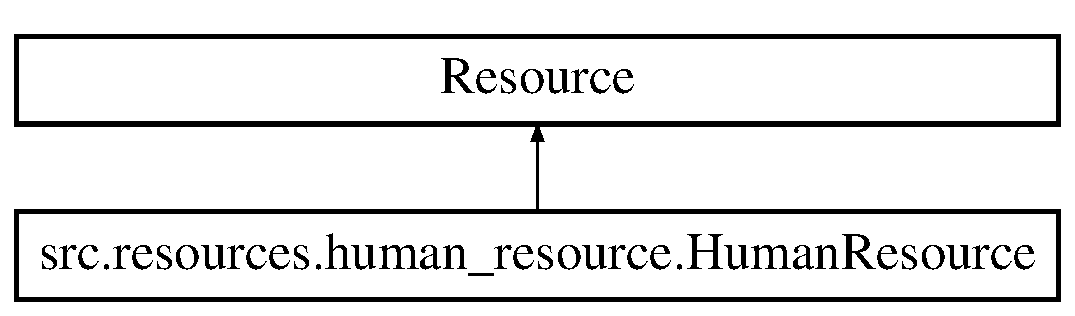
\includegraphics[height=2.000000cm]{classsrc_1_1resources_1_1human__resource_1_1_human_resource}
\end{center}
\end{figure}
\subsection*{Public Member Functions}
\begin{DoxyCompactItemize}
\item 
def \hyperlink{classsrc_1_1resources_1_1human__resource_1_1_human_resource_addeb94d9e7515701c687ddabbac2d41a}{\+\_\+\+\_\+init\+\_\+\+\_\+}
\end{DoxyCompactItemize}
\subsection*{Public Attributes}
\begin{DoxyCompactItemize}
\item 
\hyperlink{classsrc_1_1resources_1_1human__resource_1_1_human_resource_a73511a367ec14498cacc3fdb0cc77b22}{name}
\item 
\hyperlink{classsrc_1_1resources_1_1human__resource_1_1_human_resource_ad0af6551d89a2adfb08459104f46afcd}{anonymization\+Flag}
\item 
\hyperlink{classsrc_1_1resources_1_1human__resource_1_1_human_resource_a78c9919983d0f23160d8fe45732f139d}{reference}
\item 
\hyperlink{classsrc_1_1resources_1_1human__resource_1_1_human_resource_af7a5b2ee569964a16652fc96298ea6bd}{source}
\end{DoxyCompactItemize}


\subsection{Detailed Description}


Definition at line 5 of file human\+\_\+resource.\+py.



\subsection{Constructor \& Destructor Documentation}
\hypertarget{classsrc_1_1resources_1_1human__resource_1_1_human_resource_addeb94d9e7515701c687ddabbac2d41a}{\index{src\+::resources\+::human\+\_\+resource\+::\+Human\+Resource@{src\+::resources\+::human\+\_\+resource\+::\+Human\+Resource}!\+\_\+\+\_\+init\+\_\+\+\_\+@{\+\_\+\+\_\+init\+\_\+\+\_\+}}
\index{\+\_\+\+\_\+init\+\_\+\+\_\+@{\+\_\+\+\_\+init\+\_\+\+\_\+}!src\+::resources\+::human\+\_\+resource\+::\+Human\+Resource@{src\+::resources\+::human\+\_\+resource\+::\+Human\+Resource}}
\subsubsection[{\+\_\+\+\_\+init\+\_\+\+\_\+}]{\setlength{\rightskip}{0pt plus 5cm}def src.\+resources.\+human\+\_\+resource.\+Human\+Resource.\+\_\+\+\_\+init\+\_\+\+\_\+ (
\begin{DoxyParamCaption}
\item[{}]{self}
\end{DoxyParamCaption}
)}}\label{classsrc_1_1resources_1_1human__resource_1_1_human_resource_addeb94d9e7515701c687ddabbac2d41a}


Definition at line 6 of file human\+\_\+resource.\+py.



\subsection{Member Data Documentation}
\hypertarget{classsrc_1_1resources_1_1human__resource_1_1_human_resource_ad0af6551d89a2adfb08459104f46afcd}{\index{src\+::resources\+::human\+\_\+resource\+::\+Human\+Resource@{src\+::resources\+::human\+\_\+resource\+::\+Human\+Resource}!anonymization\+Flag@{anonymization\+Flag}}
\index{anonymization\+Flag@{anonymization\+Flag}!src\+::resources\+::human\+\_\+resource\+::\+Human\+Resource@{src\+::resources\+::human\+\_\+resource\+::\+Human\+Resource}}
\subsubsection[{anonymization\+Flag}]{\setlength{\rightskip}{0pt plus 5cm}src.\+resources.\+human\+\_\+resource.\+Human\+Resource.\+anonymization\+Flag}}\label{classsrc_1_1resources_1_1human__resource_1_1_human_resource_ad0af6551d89a2adfb08459104f46afcd}


Definition at line 8 of file human\+\_\+resource.\+py.

\hypertarget{classsrc_1_1resources_1_1human__resource_1_1_human_resource_a73511a367ec14498cacc3fdb0cc77b22}{\index{src\+::resources\+::human\+\_\+resource\+::\+Human\+Resource@{src\+::resources\+::human\+\_\+resource\+::\+Human\+Resource}!name@{name}}
\index{name@{name}!src\+::resources\+::human\+\_\+resource\+::\+Human\+Resource@{src\+::resources\+::human\+\_\+resource\+::\+Human\+Resource}}
\subsubsection[{name}]{\setlength{\rightskip}{0pt plus 5cm}src.\+resources.\+human\+\_\+resource.\+Human\+Resource.\+name}}\label{classsrc_1_1resources_1_1human__resource_1_1_human_resource_a73511a367ec14498cacc3fdb0cc77b22}


Definition at line 7 of file human\+\_\+resource.\+py.

\hypertarget{classsrc_1_1resources_1_1human__resource_1_1_human_resource_a78c9919983d0f23160d8fe45732f139d}{\index{src\+::resources\+::human\+\_\+resource\+::\+Human\+Resource@{src\+::resources\+::human\+\_\+resource\+::\+Human\+Resource}!reference@{reference}}
\index{reference@{reference}!src\+::resources\+::human\+\_\+resource\+::\+Human\+Resource@{src\+::resources\+::human\+\_\+resource\+::\+Human\+Resource}}
\subsubsection[{reference}]{\setlength{\rightskip}{0pt plus 5cm}src.\+resources.\+human\+\_\+resource.\+Human\+Resource.\+reference}}\label{classsrc_1_1resources_1_1human__resource_1_1_human_resource_a78c9919983d0f23160d8fe45732f139d}


Definition at line 9 of file human\+\_\+resource.\+py.

\hypertarget{classsrc_1_1resources_1_1human__resource_1_1_human_resource_af7a5b2ee569964a16652fc96298ea6bd}{\index{src\+::resources\+::human\+\_\+resource\+::\+Human\+Resource@{src\+::resources\+::human\+\_\+resource\+::\+Human\+Resource}!source@{source}}
\index{source@{source}!src\+::resources\+::human\+\_\+resource\+::\+Human\+Resource@{src\+::resources\+::human\+\_\+resource\+::\+Human\+Resource}}
\subsubsection[{source}]{\setlength{\rightskip}{0pt plus 5cm}src.\+resources.\+human\+\_\+resource.\+Human\+Resource.\+source}}\label{classsrc_1_1resources_1_1human__resource_1_1_human_resource_af7a5b2ee569964a16652fc96298ea6bd}


Definition at line 10 of file human\+\_\+resource.\+py.



The documentation for this class was generated from the following file\+:\begin{DoxyCompactItemize}
\item 
/\+Users/celine/\+Work/\+C\+N\+R\+S/workspace/\+Himal\+Co/dev/lib/lmf/src/resources/\hyperlink{human__resource_8py}{human\+\_\+resource.\+py}\end{DoxyCompactItemize}

\hypertarget{classsrc_1_1morphology_1_1lemma_1_1_lemma}{\section{src.\+morphology.\+lemma.\+Lemma Class Reference}
\label{classsrc_1_1morphology_1_1lemma_1_1_lemma}\index{src.\+morphology.\+lemma.\+Lemma@{src.\+morphology.\+lemma.\+Lemma}}
}


This class represents a lemma.  


Inheritance diagram for src.\+morphology.\+lemma.\+Lemma\+:\begin{figure}[H]
\begin{center}
\leavevmode
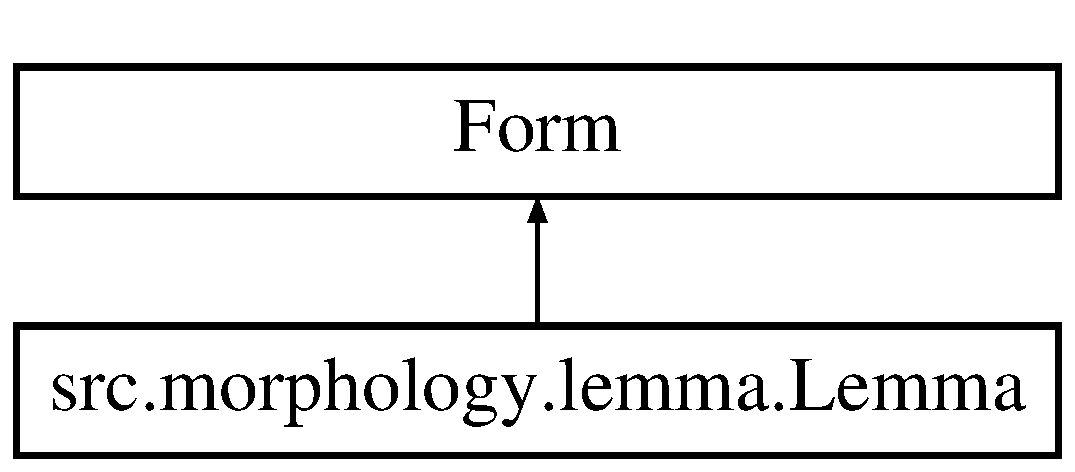
\includegraphics[height=2.000000cm]{classsrc_1_1morphology_1_1lemma_1_1_lemma}
\end{center}
\end{figure}
\subsection*{Public Member Functions}
\begin{DoxyCompactItemize}
\item 
def \hyperlink{classsrc_1_1morphology_1_1lemma_1_1_lemma_ab3860c335c5f4f9a1f05503aea52432a}{\+\_\+\+\_\+init\+\_\+\+\_\+}
\begin{DoxyCompactList}\small\item\em Constructor. \end{DoxyCompactList}\item 
def \hyperlink{classsrc_1_1morphology_1_1lemma_1_1_lemma_aa67436a851e3c33061bcce5834715be8}{set\+\_\+lexeme}
\begin{DoxyCompactList}\small\item\em Set lexeme. \end{DoxyCompactList}\item 
def \hyperlink{classsrc_1_1morphology_1_1lemma_1_1_lemma_a8b587cf5fa331a41d3ad969085b628c3}{get\+\_\+lexeme}
\begin{DoxyCompactList}\small\item\em Get lexeme. \end{DoxyCompactList}\end{DoxyCompactItemize}
\subsection*{Public Attributes}
\begin{DoxyCompactItemize}
\item 
\hyperlink{classsrc_1_1morphology_1_1lemma_1_1_lemma_a348c056c8be44e7e9b3e9c55e9973154}{hyphenation}
\item 
\hyperlink{classsrc_1_1morphology_1_1lemma_1_1_lemma_a7748c9b434cf254c617934fe550138bb}{lexeme}
\end{DoxyCompactItemize}


\subsection{Detailed Description}
This class represents a lemma. 

Definition at line 8 of file lemma.\+py.



\subsection{Constructor \& Destructor Documentation}
\hypertarget{classsrc_1_1morphology_1_1lemma_1_1_lemma_ab3860c335c5f4f9a1f05503aea52432a}{\index{src\+::morphology\+::lemma\+::\+Lemma@{src\+::morphology\+::lemma\+::\+Lemma}!\+\_\+\+\_\+init\+\_\+\+\_\+@{\+\_\+\+\_\+init\+\_\+\+\_\+}}
\index{\+\_\+\+\_\+init\+\_\+\+\_\+@{\+\_\+\+\_\+init\+\_\+\+\_\+}!src\+::morphology\+::lemma\+::\+Lemma@{src\+::morphology\+::lemma\+::\+Lemma}}
\subsubsection[{\+\_\+\+\_\+init\+\_\+\+\_\+}]{\setlength{\rightskip}{0pt plus 5cm}def src.\+morphology.\+lemma.\+Lemma.\+\_\+\+\_\+init\+\_\+\+\_\+ (
\begin{DoxyParamCaption}
\item[{}]{self}
\end{DoxyParamCaption}
)}}\label{classsrc_1_1morphology_1_1lemma_1_1_lemma_ab3860c335c5f4f9a1f05503aea52432a}


Constructor. 

\begin{DoxyReturn}{Returns}
A \hyperlink{classsrc_1_1morphology_1_1lemma_1_1_lemma}{Lemma} instance. 
\end{DoxyReturn}


Definition at line 11 of file lemma.\+py.



\subsection{Member Function Documentation}
\hypertarget{classsrc_1_1morphology_1_1lemma_1_1_lemma_a8b587cf5fa331a41d3ad969085b628c3}{\index{src\+::morphology\+::lemma\+::\+Lemma@{src\+::morphology\+::lemma\+::\+Lemma}!get\+\_\+lexeme@{get\+\_\+lexeme}}
\index{get\+\_\+lexeme@{get\+\_\+lexeme}!src\+::morphology\+::lemma\+::\+Lemma@{src\+::morphology\+::lemma\+::\+Lemma}}
\subsubsection[{get\+\_\+lexeme}]{\setlength{\rightskip}{0pt plus 5cm}def src.\+morphology.\+lemma.\+Lemma.\+get\+\_\+lexeme (
\begin{DoxyParamCaption}
\item[{}]{self}
\end{DoxyParamCaption}
)}}\label{classsrc_1_1morphology_1_1lemma_1_1_lemma_a8b587cf5fa331a41d3ad969085b628c3}


Get lexeme. 

\begin{DoxyReturn}{Returns}
\hyperlink{classsrc_1_1morphology_1_1lemma_1_1_lemma}{Lemma} attribute 'lexeme'. 
\end{DoxyReturn}


Definition at line 26 of file lemma.\+py.

\hypertarget{classsrc_1_1morphology_1_1lemma_1_1_lemma_aa67436a851e3c33061bcce5834715be8}{\index{src\+::morphology\+::lemma\+::\+Lemma@{src\+::morphology\+::lemma\+::\+Lemma}!set\+\_\+lexeme@{set\+\_\+lexeme}}
\index{set\+\_\+lexeme@{set\+\_\+lexeme}!src\+::morphology\+::lemma\+::\+Lemma@{src\+::morphology\+::lemma\+::\+Lemma}}
\subsubsection[{set\+\_\+lexeme}]{\setlength{\rightskip}{0pt plus 5cm}def src.\+morphology.\+lemma.\+Lemma.\+set\+\_\+lexeme (
\begin{DoxyParamCaption}
\item[{}]{self, }
\item[{}]{lexeme}
\end{DoxyParamCaption}
)}}\label{classsrc_1_1morphology_1_1lemma_1_1_lemma_aa67436a851e3c33061bcce5834715be8}


Set lexeme. 


\begin{DoxyParams}{Parameters}
{\em lexeme} & The lexeme to set. \\
\hline
\end{DoxyParams}
\begin{DoxyReturn}{Returns}
\hyperlink{classsrc_1_1morphology_1_1lemma_1_1_lemma}{Lemma} instance. 
\end{DoxyReturn}


Definition at line 18 of file lemma.\+py.



\subsection{Member Data Documentation}
\hypertarget{classsrc_1_1morphology_1_1lemma_1_1_lemma_a348c056c8be44e7e9b3e9c55e9973154}{\index{src\+::morphology\+::lemma\+::\+Lemma@{src\+::morphology\+::lemma\+::\+Lemma}!hyphenation@{hyphenation}}
\index{hyphenation@{hyphenation}!src\+::morphology\+::lemma\+::\+Lemma@{src\+::morphology\+::lemma\+::\+Lemma}}
\subsubsection[{hyphenation}]{\setlength{\rightskip}{0pt plus 5cm}src.\+morphology.\+lemma.\+Lemma.\+hyphenation}}\label{classsrc_1_1morphology_1_1lemma_1_1_lemma_a348c056c8be44e7e9b3e9c55e9973154}


Definition at line 15 of file lemma.\+py.

\hypertarget{classsrc_1_1morphology_1_1lemma_1_1_lemma_a7748c9b434cf254c617934fe550138bb}{\index{src\+::morphology\+::lemma\+::\+Lemma@{src\+::morphology\+::lemma\+::\+Lemma}!lexeme@{lexeme}}
\index{lexeme@{lexeme}!src\+::morphology\+::lemma\+::\+Lemma@{src\+::morphology\+::lemma\+::\+Lemma}}
\subsubsection[{lexeme}]{\setlength{\rightskip}{0pt plus 5cm}src.\+morphology.\+lemma.\+Lemma.\+lexeme}}\label{classsrc_1_1morphology_1_1lemma_1_1_lemma_a7748c9b434cf254c617934fe550138bb}


Definition at line 16 of file lemma.\+py.



The documentation for this class was generated from the following file\+:\begin{DoxyCompactItemize}
\item 
/\+Users/celine/\+Work/\+C\+N\+R\+S/workspace/\+Himal\+Co/dev/lib/lmf/src/morphology/\hyperlink{lemma_8py}{lemma.\+py}\end{DoxyCompactItemize}

\hypertarget{classsrc_1_1core_1_1lexical__entry_1_1_lexical_entry}{\section{src.\+core.\+lexical\+\_\+entry.\+Lexical\+Entry Class Reference}
\label{classsrc_1_1core_1_1lexical__entry_1_1_lexical_entry}\index{src.\+core.\+lexical\+\_\+entry.\+Lexical\+Entry@{src.\+core.\+lexical\+\_\+entry.\+Lexical\+Entry}}
}


This class represents a lexical entry.  


\subsection*{Public Member Functions}
\begin{DoxyCompactItemize}
\item 
def \hyperlink{classsrc_1_1core_1_1lexical__entry_1_1_lexical_entry_ad07b137971a11c6c47b713d73453711a}{\+\_\+\+\_\+init\+\_\+\+\_\+}
\begin{DoxyCompactList}\small\item\em Constructor. \end{DoxyCompactList}\item 
def \hyperlink{classsrc_1_1core_1_1lexical__entry_1_1_lexical_entry_a8a612b39c5eebb3ee3d5deffbb3b2fda}{set\+\_\+part\+Of\+Speech}
\begin{DoxyCompactList}\small\item\em Set grammatical category. \end{DoxyCompactList}\item 
def \hyperlink{classsrc_1_1core_1_1lexical__entry_1_1_lexical_entry_ad5c7bc9ada1f19b0ca45a645d8dbab82}{get\+\_\+part\+Of\+Speech}
\begin{DoxyCompactList}\small\item\em Get grammatical category. \end{DoxyCompactList}\item 
def \hyperlink{classsrc_1_1core_1_1lexical__entry_1_1_lexical_entry_a73f06145dc2f2d50eb7c62d0604f5b69}{set\+\_\+status}
\begin{DoxyCompactList}\small\item\em Set lexical entry status. \end{DoxyCompactList}\item 
def \hyperlink{classsrc_1_1core_1_1lexical__entry_1_1_lexical_entry_a7657aabb009cb71d94f8f5abd67e2ed4}{get\+\_\+status}
\begin{DoxyCompactList}\small\item\em Get lexical entry status. \end{DoxyCompactList}\item 
def \hyperlink{classsrc_1_1core_1_1lexical__entry_1_1_lexical_entry_a5caac60aebc0855ed5a1522bca0d5f0e}{get\+\_\+id}
\begin{DoxyCompactList}\small\item\em Get Unique I\+Dentifier. \end{DoxyCompactList}\item 
def \hyperlink{classsrc_1_1core_1_1lexical__entry_1_1_lexical_entry_a0dcb24c70fdad0cc4ed49d8c18d7e93d}{set\+\_\+lexeme}
\begin{DoxyCompactList}\small\item\em Set lexeme. \end{DoxyCompactList}\item 
def \hyperlink{classsrc_1_1core_1_1lexical__entry_1_1_lexical_entry_a3a816168935e5601847decc2036cf1ee}{get\+\_\+lexeme}
\begin{DoxyCompactList}\small\item\em Get lexeme. \end{DoxyCompactList}\end{DoxyCompactItemize}
\subsection*{Public Attributes}
\begin{DoxyCompactItemize}
\item 
\hyperlink{classsrc_1_1core_1_1lexical__entry_1_1_lexical_entry_aa7a1e19f555ab214c4c4280fefe84bff}{homonym\+Number}
\item 
\hyperlink{classsrc_1_1core_1_1lexical__entry_1_1_lexical_entry_a661ab019b1e1fde2f86158a566eba3fd}{status}
\item 
\hyperlink{classsrc_1_1core_1_1lexical__entry_1_1_lexical_entry_aaa4dae2afec96335786b54c8d5b5f12e}{date}
\item 
\hyperlink{classsrc_1_1core_1_1lexical__entry_1_1_lexical_entry_a9f7833c971ca31885d3d7383fb394d03}{part\+Of\+Speech}
\item 
\hyperlink{classsrc_1_1core_1_1lexical__entry_1_1_lexical_entry_a93614de55bcf2c644c9c048812e318f8}{independent\+Word}
\item 
\hyperlink{classsrc_1_1core_1_1lexical__entry_1_1_lexical_entry_a9f128ce8e68efcbab65b4163a56ab0dd}{bibliography}
\item 
\hyperlink{classsrc_1_1core_1_1lexical__entry_1_1_lexical_entry_a210b91bf8efc402f897e4a62b9e24341}{id}
\begin{DoxyCompactList}\small\item\em Unique I\+Dentifier is managed at the Lexicon level. \end{DoxyCompactList}\item 
\hyperlink{classsrc_1_1core_1_1lexical__entry_1_1_lexical_entry_a616298be2e81b660fc8e6eccd7c4dcfb}{lemma}
\begin{DoxyCompactList}\small\item\em Lemma instance is owned by \hyperlink{classsrc_1_1core_1_1lexical__entry_1_1_lexical_entry}{Lexical\+Entry} There is one Lemma instance by \hyperlink{classsrc_1_1core_1_1lexical__entry_1_1_lexical_entry}{Lexical\+Entry} instance. \end{DoxyCompactList}\end{DoxyCompactItemize}


\subsection{Detailed Description}
This class represents a lexical entry. 

Definition at line 8 of file lexical\+\_\+entry.\+py.



\subsection{Constructor \& Destructor Documentation}
\hypertarget{classsrc_1_1core_1_1lexical__entry_1_1_lexical_entry_ad07b137971a11c6c47b713d73453711a}{\index{src\+::core\+::lexical\+\_\+entry\+::\+Lexical\+Entry@{src\+::core\+::lexical\+\_\+entry\+::\+Lexical\+Entry}!\+\_\+\+\_\+init\+\_\+\+\_\+@{\+\_\+\+\_\+init\+\_\+\+\_\+}}
\index{\+\_\+\+\_\+init\+\_\+\+\_\+@{\+\_\+\+\_\+init\+\_\+\+\_\+}!src\+::core\+::lexical\+\_\+entry\+::\+Lexical\+Entry@{src\+::core\+::lexical\+\_\+entry\+::\+Lexical\+Entry}}
\subsubsection[{\+\_\+\+\_\+init\+\_\+\+\_\+}]{\setlength{\rightskip}{0pt plus 5cm}def src.\+core.\+lexical\+\_\+entry.\+Lexical\+Entry.\+\_\+\+\_\+init\+\_\+\+\_\+ (
\begin{DoxyParamCaption}
\item[{}]{self}
\end{DoxyParamCaption}
)}}\label{classsrc_1_1core_1_1lexical__entry_1_1_lexical_entry_ad07b137971a11c6c47b713d73453711a}


Constructor. 

\begin{DoxyReturn}{Returns}
A \hyperlink{classsrc_1_1core_1_1lexical__entry_1_1_lexical_entry}{Lexical\+Entry} instance. 
\end{DoxyReturn}


Definition at line 11 of file lexical\+\_\+entry.\+py.



\subsection{Member Function Documentation}
\hypertarget{classsrc_1_1core_1_1lexical__entry_1_1_lexical_entry_a5caac60aebc0855ed5a1522bca0d5f0e}{\index{src\+::core\+::lexical\+\_\+entry\+::\+Lexical\+Entry@{src\+::core\+::lexical\+\_\+entry\+::\+Lexical\+Entry}!get\+\_\+id@{get\+\_\+id}}
\index{get\+\_\+id@{get\+\_\+id}!src\+::core\+::lexical\+\_\+entry\+::\+Lexical\+Entry@{src\+::core\+::lexical\+\_\+entry\+::\+Lexical\+Entry}}
\subsubsection[{get\+\_\+id}]{\setlength{\rightskip}{0pt plus 5cm}def src.\+core.\+lexical\+\_\+entry.\+Lexical\+Entry.\+get\+\_\+id (
\begin{DoxyParamCaption}
\item[{}]{self}
\end{DoxyParamCaption}
)}}\label{classsrc_1_1core_1_1lexical__entry_1_1_lexical_entry_a5caac60aebc0855ed5a1522bca0d5f0e}


Get Unique I\+Dentifier. 

\begin{DoxyReturn}{Returns}
\hyperlink{classsrc_1_1core_1_1lexical__entry_1_1_lexical_entry}{Lexical\+Entry} attribute 'id'. 
\end{DoxyReturn}


Definition at line 55 of file lexical\+\_\+entry.\+py.

\hypertarget{classsrc_1_1core_1_1lexical__entry_1_1_lexical_entry_a3a816168935e5601847decc2036cf1ee}{\index{src\+::core\+::lexical\+\_\+entry\+::\+Lexical\+Entry@{src\+::core\+::lexical\+\_\+entry\+::\+Lexical\+Entry}!get\+\_\+lexeme@{get\+\_\+lexeme}}
\index{get\+\_\+lexeme@{get\+\_\+lexeme}!src\+::core\+::lexical\+\_\+entry\+::\+Lexical\+Entry@{src\+::core\+::lexical\+\_\+entry\+::\+Lexical\+Entry}}
\subsubsection[{get\+\_\+lexeme}]{\setlength{\rightskip}{0pt plus 5cm}def src.\+core.\+lexical\+\_\+entry.\+Lexical\+Entry.\+get\+\_\+lexeme (
\begin{DoxyParamCaption}
\item[{}]{self}
\end{DoxyParamCaption}
)}}\label{classsrc_1_1core_1_1lexical__entry_1_1_lexical_entry_a3a816168935e5601847decc2036cf1ee}


Get lexeme. 

Attribute 'lexeme' is owned by Lemma. \begin{DoxyReturn}{Returns}
Lemma attribute 'lexeme' if any. 
\end{DoxyReturn}


Definition at line 72 of file lexical\+\_\+entry.\+py.

\hypertarget{classsrc_1_1core_1_1lexical__entry_1_1_lexical_entry_ad5c7bc9ada1f19b0ca45a645d8dbab82}{\index{src\+::core\+::lexical\+\_\+entry\+::\+Lexical\+Entry@{src\+::core\+::lexical\+\_\+entry\+::\+Lexical\+Entry}!get\+\_\+part\+Of\+Speech@{get\+\_\+part\+Of\+Speech}}
\index{get\+\_\+part\+Of\+Speech@{get\+\_\+part\+Of\+Speech}!src\+::core\+::lexical\+\_\+entry\+::\+Lexical\+Entry@{src\+::core\+::lexical\+\_\+entry\+::\+Lexical\+Entry}}
\subsubsection[{get\+\_\+part\+Of\+Speech}]{\setlength{\rightskip}{0pt plus 5cm}def src.\+core.\+lexical\+\_\+entry.\+Lexical\+Entry.\+get\+\_\+part\+Of\+Speech (
\begin{DoxyParamCaption}
\item[{}]{self}
\end{DoxyParamCaption}
)}}\label{classsrc_1_1core_1_1lexical__entry_1_1_lexical_entry_ad5c7bc9ada1f19b0ca45a645d8dbab82}


Get grammatical category. 

\begin{DoxyReturn}{Returns}
\hyperlink{classsrc_1_1core_1_1lexical__entry_1_1_lexical_entry}{Lexical\+Entry} attribute 'part\+Of\+Speech'. 
\end{DoxyReturn}


Definition at line 35 of file lexical\+\_\+entry.\+py.

\hypertarget{classsrc_1_1core_1_1lexical__entry_1_1_lexical_entry_a7657aabb009cb71d94f8f5abd67e2ed4}{\index{src\+::core\+::lexical\+\_\+entry\+::\+Lexical\+Entry@{src\+::core\+::lexical\+\_\+entry\+::\+Lexical\+Entry}!get\+\_\+status@{get\+\_\+status}}
\index{get\+\_\+status@{get\+\_\+status}!src\+::core\+::lexical\+\_\+entry\+::\+Lexical\+Entry@{src\+::core\+::lexical\+\_\+entry\+::\+Lexical\+Entry}}
\subsubsection[{get\+\_\+status}]{\setlength{\rightskip}{0pt plus 5cm}def src.\+core.\+lexical\+\_\+entry.\+Lexical\+Entry.\+get\+\_\+status (
\begin{DoxyParamCaption}
\item[{}]{self}
\end{DoxyParamCaption}
)}}\label{classsrc_1_1core_1_1lexical__entry_1_1_lexical_entry_a7657aabb009cb71d94f8f5abd67e2ed4}


Get lexical entry status. 

\begin{DoxyReturn}{Returns}
\hyperlink{classsrc_1_1core_1_1lexical__entry_1_1_lexical_entry}{Lexical\+Entry} attribute 'status'. 
\end{DoxyReturn}


Definition at line 49 of file lexical\+\_\+entry.\+py.

\hypertarget{classsrc_1_1core_1_1lexical__entry_1_1_lexical_entry_a0dcb24c70fdad0cc4ed49d8c18d7e93d}{\index{src\+::core\+::lexical\+\_\+entry\+::\+Lexical\+Entry@{src\+::core\+::lexical\+\_\+entry\+::\+Lexical\+Entry}!set\+\_\+lexeme@{set\+\_\+lexeme}}
\index{set\+\_\+lexeme@{set\+\_\+lexeme}!src\+::core\+::lexical\+\_\+entry\+::\+Lexical\+Entry@{src\+::core\+::lexical\+\_\+entry\+::\+Lexical\+Entry}}
\subsubsection[{set\+\_\+lexeme}]{\setlength{\rightskip}{0pt plus 5cm}def src.\+core.\+lexical\+\_\+entry.\+Lexical\+Entry.\+set\+\_\+lexeme (
\begin{DoxyParamCaption}
\item[{}]{self, }
\item[{}]{lexeme}
\end{DoxyParamCaption}
)}}\label{classsrc_1_1core_1_1lexical__entry_1_1_lexical_entry_a0dcb24c70fdad0cc4ed49d8c18d7e93d}


Set lexeme. 

Attribute 'lexeme' is owned by Lemma. 
\begin{DoxyParams}{Parameters}
{\em lexeme} & The lexeme to set. \\
\hline
\end{DoxyParams}


Definition at line 61 of file lexical\+\_\+entry.\+py.

\hypertarget{classsrc_1_1core_1_1lexical__entry_1_1_lexical_entry_a8a612b39c5eebb3ee3d5deffbb3b2fda}{\index{src\+::core\+::lexical\+\_\+entry\+::\+Lexical\+Entry@{src\+::core\+::lexical\+\_\+entry\+::\+Lexical\+Entry}!set\+\_\+part\+Of\+Speech@{set\+\_\+part\+Of\+Speech}}
\index{set\+\_\+part\+Of\+Speech@{set\+\_\+part\+Of\+Speech}!src\+::core\+::lexical\+\_\+entry\+::\+Lexical\+Entry@{src\+::core\+::lexical\+\_\+entry\+::\+Lexical\+Entry}}
\subsubsection[{set\+\_\+part\+Of\+Speech}]{\setlength{\rightskip}{0pt plus 5cm}def src.\+core.\+lexical\+\_\+entry.\+Lexical\+Entry.\+set\+\_\+part\+Of\+Speech (
\begin{DoxyParamCaption}
\item[{}]{self, }
\item[{}]{part\+\_\+of\+\_\+speech}
\end{DoxyParamCaption}
)}}\label{classsrc_1_1core_1_1lexical__entry_1_1_lexical_entry_a8a612b39c5eebb3ee3d5deffbb3b2fda}


Set grammatical category. 


\begin{DoxyParams}{Parameters}
{\em part\+\_\+of\+\_\+speech} & The grammatical category to set. \\
\hline
\end{DoxyParams}
\begin{DoxyReturn}{Returns}
\hyperlink{classsrc_1_1core_1_1lexical__entry_1_1_lexical_entry}{Lexical\+Entry} instance. 
\end{DoxyReturn}


Definition at line 27 of file lexical\+\_\+entry.\+py.

\hypertarget{classsrc_1_1core_1_1lexical__entry_1_1_lexical_entry_a73f06145dc2f2d50eb7c62d0604f5b69}{\index{src\+::core\+::lexical\+\_\+entry\+::\+Lexical\+Entry@{src\+::core\+::lexical\+\_\+entry\+::\+Lexical\+Entry}!set\+\_\+status@{set\+\_\+status}}
\index{set\+\_\+status@{set\+\_\+status}!src\+::core\+::lexical\+\_\+entry\+::\+Lexical\+Entry@{src\+::core\+::lexical\+\_\+entry\+::\+Lexical\+Entry}}
\subsubsection[{set\+\_\+status}]{\setlength{\rightskip}{0pt plus 5cm}def src.\+core.\+lexical\+\_\+entry.\+Lexical\+Entry.\+set\+\_\+status (
\begin{DoxyParamCaption}
\item[{}]{self, }
\item[{}]{status}
\end{DoxyParamCaption}
)}}\label{classsrc_1_1core_1_1lexical__entry_1_1_lexical_entry_a73f06145dc2f2d50eb7c62d0604f5b69}


Set lexical entry status. 


\begin{DoxyParams}{Parameters}
{\em status} & The status to set. \\
\hline
\end{DoxyParams}
\begin{DoxyReturn}{Returns}
\hyperlink{classsrc_1_1core_1_1lexical__entry_1_1_lexical_entry}{Lexical\+Entry} instance. 
\end{DoxyReturn}


Definition at line 41 of file lexical\+\_\+entry.\+py.



\subsection{Member Data Documentation}
\hypertarget{classsrc_1_1core_1_1lexical__entry_1_1_lexical_entry_a9f128ce8e68efcbab65b4163a56ab0dd}{\index{src\+::core\+::lexical\+\_\+entry\+::\+Lexical\+Entry@{src\+::core\+::lexical\+\_\+entry\+::\+Lexical\+Entry}!bibliography@{bibliography}}
\index{bibliography@{bibliography}!src\+::core\+::lexical\+\_\+entry\+::\+Lexical\+Entry@{src\+::core\+::lexical\+\_\+entry\+::\+Lexical\+Entry}}
\subsubsection[{bibliography}]{\setlength{\rightskip}{0pt plus 5cm}src.\+core.\+lexical\+\_\+entry.\+Lexical\+Entry.\+bibliography}}\label{classsrc_1_1core_1_1lexical__entry_1_1_lexical_entry_a9f128ce8e68efcbab65b4163a56ab0dd}


Definition at line 20 of file lexical\+\_\+entry.\+py.

\hypertarget{classsrc_1_1core_1_1lexical__entry_1_1_lexical_entry_aaa4dae2afec96335786b54c8d5b5f12e}{\index{src\+::core\+::lexical\+\_\+entry\+::\+Lexical\+Entry@{src\+::core\+::lexical\+\_\+entry\+::\+Lexical\+Entry}!date@{date}}
\index{date@{date}!src\+::core\+::lexical\+\_\+entry\+::\+Lexical\+Entry@{src\+::core\+::lexical\+\_\+entry\+::\+Lexical\+Entry}}
\subsubsection[{date}]{\setlength{\rightskip}{0pt plus 5cm}src.\+core.\+lexical\+\_\+entry.\+Lexical\+Entry.\+date}}\label{classsrc_1_1core_1_1lexical__entry_1_1_lexical_entry_aaa4dae2afec96335786b54c8d5b5f12e}


Definition at line 17 of file lexical\+\_\+entry.\+py.

\hypertarget{classsrc_1_1core_1_1lexical__entry_1_1_lexical_entry_aa7a1e19f555ab214c4c4280fefe84bff}{\index{src\+::core\+::lexical\+\_\+entry\+::\+Lexical\+Entry@{src\+::core\+::lexical\+\_\+entry\+::\+Lexical\+Entry}!homonym\+Number@{homonym\+Number}}
\index{homonym\+Number@{homonym\+Number}!src\+::core\+::lexical\+\_\+entry\+::\+Lexical\+Entry@{src\+::core\+::lexical\+\_\+entry\+::\+Lexical\+Entry}}
\subsubsection[{homonym\+Number}]{\setlength{\rightskip}{0pt plus 5cm}src.\+core.\+lexical\+\_\+entry.\+Lexical\+Entry.\+homonym\+Number}}\label{classsrc_1_1core_1_1lexical__entry_1_1_lexical_entry_aa7a1e19f555ab214c4c4280fefe84bff}


Definition at line 15 of file lexical\+\_\+entry.\+py.

\hypertarget{classsrc_1_1core_1_1lexical__entry_1_1_lexical_entry_a210b91bf8efc402f897e4a62b9e24341}{\index{src\+::core\+::lexical\+\_\+entry\+::\+Lexical\+Entry@{src\+::core\+::lexical\+\_\+entry\+::\+Lexical\+Entry}!id@{id}}
\index{id@{id}!src\+::core\+::lexical\+\_\+entry\+::\+Lexical\+Entry@{src\+::core\+::lexical\+\_\+entry\+::\+Lexical\+Entry}}
\subsubsection[{id}]{\setlength{\rightskip}{0pt plus 5cm}src.\+core.\+lexical\+\_\+entry.\+Lexical\+Entry.\+id}}\label{classsrc_1_1core_1_1lexical__entry_1_1_lexical_entry_a210b91bf8efc402f897e4a62b9e24341}


Unique I\+Dentifier is managed at the Lexicon level. 



Definition at line 22 of file lexical\+\_\+entry.\+py.

\hypertarget{classsrc_1_1core_1_1lexical__entry_1_1_lexical_entry_a93614de55bcf2c644c9c048812e318f8}{\index{src\+::core\+::lexical\+\_\+entry\+::\+Lexical\+Entry@{src\+::core\+::lexical\+\_\+entry\+::\+Lexical\+Entry}!independent\+Word@{independent\+Word}}
\index{independent\+Word@{independent\+Word}!src\+::core\+::lexical\+\_\+entry\+::\+Lexical\+Entry@{src\+::core\+::lexical\+\_\+entry\+::\+Lexical\+Entry}}
\subsubsection[{independent\+Word}]{\setlength{\rightskip}{0pt plus 5cm}src.\+core.\+lexical\+\_\+entry.\+Lexical\+Entry.\+independent\+Word}}\label{classsrc_1_1core_1_1lexical__entry_1_1_lexical_entry_a93614de55bcf2c644c9c048812e318f8}


Definition at line 19 of file lexical\+\_\+entry.\+py.

\hypertarget{classsrc_1_1core_1_1lexical__entry_1_1_lexical_entry_a616298be2e81b660fc8e6eccd7c4dcfb}{\index{src\+::core\+::lexical\+\_\+entry\+::\+Lexical\+Entry@{src\+::core\+::lexical\+\_\+entry\+::\+Lexical\+Entry}!lemma@{lemma}}
\index{lemma@{lemma}!src\+::core\+::lexical\+\_\+entry\+::\+Lexical\+Entry@{src\+::core\+::lexical\+\_\+entry\+::\+Lexical\+Entry}}
\subsubsection[{lemma}]{\setlength{\rightskip}{0pt plus 5cm}src.\+core.\+lexical\+\_\+entry.\+Lexical\+Entry.\+lemma}}\label{classsrc_1_1core_1_1lexical__entry_1_1_lexical_entry_a616298be2e81b660fc8e6eccd7c4dcfb}


Lemma instance is owned by \hyperlink{classsrc_1_1core_1_1lexical__entry_1_1_lexical_entry}{Lexical\+Entry} There is one Lemma instance by \hyperlink{classsrc_1_1core_1_1lexical__entry_1_1_lexical_entry}{Lexical\+Entry} instance. 



Definition at line 25 of file lexical\+\_\+entry.\+py.

\hypertarget{classsrc_1_1core_1_1lexical__entry_1_1_lexical_entry_a9f7833c971ca31885d3d7383fb394d03}{\index{src\+::core\+::lexical\+\_\+entry\+::\+Lexical\+Entry@{src\+::core\+::lexical\+\_\+entry\+::\+Lexical\+Entry}!part\+Of\+Speech@{part\+Of\+Speech}}
\index{part\+Of\+Speech@{part\+Of\+Speech}!src\+::core\+::lexical\+\_\+entry\+::\+Lexical\+Entry@{src\+::core\+::lexical\+\_\+entry\+::\+Lexical\+Entry}}
\subsubsection[{part\+Of\+Speech}]{\setlength{\rightskip}{0pt plus 5cm}src.\+core.\+lexical\+\_\+entry.\+Lexical\+Entry.\+part\+Of\+Speech}}\label{classsrc_1_1core_1_1lexical__entry_1_1_lexical_entry_a9f7833c971ca31885d3d7383fb394d03}


Definition at line 18 of file lexical\+\_\+entry.\+py.

\hypertarget{classsrc_1_1core_1_1lexical__entry_1_1_lexical_entry_a661ab019b1e1fde2f86158a566eba3fd}{\index{src\+::core\+::lexical\+\_\+entry\+::\+Lexical\+Entry@{src\+::core\+::lexical\+\_\+entry\+::\+Lexical\+Entry}!status@{status}}
\index{status@{status}!src\+::core\+::lexical\+\_\+entry\+::\+Lexical\+Entry@{src\+::core\+::lexical\+\_\+entry\+::\+Lexical\+Entry}}
\subsubsection[{status}]{\setlength{\rightskip}{0pt plus 5cm}src.\+core.\+lexical\+\_\+entry.\+Lexical\+Entry.\+status}}\label{classsrc_1_1core_1_1lexical__entry_1_1_lexical_entry_a661ab019b1e1fde2f86158a566eba3fd}


Definition at line 16 of file lexical\+\_\+entry.\+py.



The documentation for this class was generated from the following file\+:\begin{DoxyCompactItemize}
\item 
/\+Users/celine/\+Work/\+C\+N\+R\+S/workspace/\+Himal\+Co/dev/lib/lmf/src/core/\hyperlink{lexical__entry_8py}{lexical\+\_\+entry.\+py}\end{DoxyCompactItemize}

\hypertarget{classsrc_1_1core_1_1lexical__resource_1_1_lexical_resource}{\section{src.\+core.\+lexical\+\_\+resource.\+Lexical\+Resource Class Reference}
\label{classsrc_1_1core_1_1lexical__resource_1_1_lexical_resource}\index{src.\+core.\+lexical\+\_\+resource.\+Lexical\+Resource@{src.\+core.\+lexical\+\_\+resource.\+Lexical\+Resource}}
}
\subsection*{Public Member Functions}
\begin{DoxyCompactItemize}
\item 
def \hyperlink{classsrc_1_1core_1_1lexical__resource_1_1_lexical_resource_a0915db40dd08736e7654cb4c7aaf2456}{\+\_\+\+\_\+init\+\_\+\+\_\+}
\end{DoxyCompactItemize}
\subsection*{Public Attributes}
\begin{DoxyCompactItemize}
\item 
\hyperlink{classsrc_1_1core_1_1lexical__resource_1_1_lexical_resource_a8c8a0a171fe52f3ef8db4a58898ece0f}{dtd\+Version}
\end{DoxyCompactItemize}


\subsection{Detailed Description}


Definition at line 3 of file lexical\+\_\+resource.\+py.



\subsection{Constructor \& Destructor Documentation}
\hypertarget{classsrc_1_1core_1_1lexical__resource_1_1_lexical_resource_a0915db40dd08736e7654cb4c7aaf2456}{\index{src\+::core\+::lexical\+\_\+resource\+::\+Lexical\+Resource@{src\+::core\+::lexical\+\_\+resource\+::\+Lexical\+Resource}!\+\_\+\+\_\+init\+\_\+\+\_\+@{\+\_\+\+\_\+init\+\_\+\+\_\+}}
\index{\+\_\+\+\_\+init\+\_\+\+\_\+@{\+\_\+\+\_\+init\+\_\+\+\_\+}!src\+::core\+::lexical\+\_\+resource\+::\+Lexical\+Resource@{src\+::core\+::lexical\+\_\+resource\+::\+Lexical\+Resource}}
\subsubsection[{\+\_\+\+\_\+init\+\_\+\+\_\+}]{\setlength{\rightskip}{0pt plus 5cm}def src.\+core.\+lexical\+\_\+resource.\+Lexical\+Resource.\+\_\+\+\_\+init\+\_\+\+\_\+ (
\begin{DoxyParamCaption}
\item[{}]{self}
\end{DoxyParamCaption}
)}}\label{classsrc_1_1core_1_1lexical__resource_1_1_lexical_resource_a0915db40dd08736e7654cb4c7aaf2456}


Definition at line 4 of file lexical\+\_\+resource.\+py.



\subsection{Member Data Documentation}
\hypertarget{classsrc_1_1core_1_1lexical__resource_1_1_lexical_resource_a8c8a0a171fe52f3ef8db4a58898ece0f}{\index{src\+::core\+::lexical\+\_\+resource\+::\+Lexical\+Resource@{src\+::core\+::lexical\+\_\+resource\+::\+Lexical\+Resource}!dtd\+Version@{dtd\+Version}}
\index{dtd\+Version@{dtd\+Version}!src\+::core\+::lexical\+\_\+resource\+::\+Lexical\+Resource@{src\+::core\+::lexical\+\_\+resource\+::\+Lexical\+Resource}}
\subsubsection[{dtd\+Version}]{\setlength{\rightskip}{0pt plus 5cm}src.\+core.\+lexical\+\_\+resource.\+Lexical\+Resource.\+dtd\+Version}}\label{classsrc_1_1core_1_1lexical__resource_1_1_lexical_resource_a8c8a0a171fe52f3ef8db4a58898ece0f}


Definition at line 5 of file lexical\+\_\+resource.\+py.



The documentation for this class was generated from the following file\+:\begin{DoxyCompactItemize}
\item 
/\+Users/celine/\+Work/\+C\+N\+R\+S/workspace/\+Himal\+Co/dev/lib/lmf/src/core/\hyperlink{lexical__resource_8py}{lexical\+\_\+resource.\+py}\end{DoxyCompactItemize}

\hypertarget{classsrc_1_1core_1_1lexicon_1_1_lexicon}{\section{src.\+core.\+lexicon.\+Lexicon Class Reference}
\label{classsrc_1_1core_1_1lexicon_1_1_lexicon}\index{src.\+core.\+lexicon.\+Lexicon@{src.\+core.\+lexicon.\+Lexicon}}
}


This class represents a lexicon containing lexical entries.  


\subsection*{Public Member Functions}
\begin{DoxyCompactItemize}
\item 
def \hyperlink{classsrc_1_1core_1_1lexicon_1_1_lexicon_a4e1bde14f0dab23d8b6462beb438a3b8}{\+\_\+\+\_\+init\+\_\+\+\_\+}
\begin{DoxyCompactList}\small\item\em Constructor. \end{DoxyCompactList}\item 
def \hyperlink{classsrc_1_1core_1_1lexicon_1_1_lexicon_ab86f6df343dcce5256e00df0876d00dc}{get\+\_\+lexical\+\_\+entries}
\begin{DoxyCompactList}\small\item\em Get all lexical entries maintained by the lexicon. \end{DoxyCompactList}\item 
def \hyperlink{classsrc_1_1core_1_1lexicon_1_1_lexicon_ae07f5ea7bb47595d8f0559910663c66e}{add\+\_\+lexical\+\_\+entry}
\begin{DoxyCompactList}\small\item\em Add a lexical entry to the lexicon. \end{DoxyCompactList}\item 
def \hyperlink{classsrc_1_1core_1_1lexicon_1_1_lexicon_a50ea2e94e8faf8d4d653695cd573af06}{remove\+\_\+lexical\+\_\+entry}
\begin{DoxyCompactList}\small\item\em Remove a lexical entry from the lexicon. \end{DoxyCompactList}\item 
def \hyperlink{classsrc_1_1core_1_1lexicon_1_1_lexicon_ab3f928e814243282a8dc81745cc3b8a5}{count\+\_\+lexical\+\_\+entries}
\begin{DoxyCompactList}\small\item\em Count number of lexical entries of the lexicon. \end{DoxyCompactList}\item 
def \hyperlink{classsrc_1_1core_1_1lexicon_1_1_lexicon_a650614d631962184f7aeca94569c6245}{sort\+\_\+lexical\+\_\+entries}
\begin{DoxyCompactList}\small\item\em Sort given items of lexical entries contained in the lexicon according to a certain order. \end{DoxyCompactList}\end{DoxyCompactItemize}
\subsection*{Public Attributes}
\begin{DoxyCompactItemize}
\item 
\hyperlink{classsrc_1_1core_1_1lexicon_1_1_lexicon_a142d9d1c45eac0ece70b80c5a8033b02}{language}
\item 
\hyperlink{classsrc_1_1core_1_1lexicon_1_1_lexicon_a0e5ff6cffd788ae4ca6bdd069c6938ba}{language\+Script}
\item 
\hyperlink{classsrc_1_1core_1_1lexicon_1_1_lexicon_ac76ee39a545b73a67d005b00645ec7cc}{id}
\item 
\hyperlink{classsrc_1_1core_1_1lexicon_1_1_lexicon_a478e60c805dd1d5bc4e2bf7f3b5c8be0}{label}
\item 
\hyperlink{classsrc_1_1core_1_1lexicon_1_1_lexicon_a1e0df327bd01235e6e38a214584cef5d}{lexicon\+Type}
\item 
\hyperlink{classsrc_1_1core_1_1lexicon_1_1_lexicon_a0d7e1062a1ed7788520c7db08e8b1d40}{entry\+Source}
\item 
\hyperlink{classsrc_1_1core_1_1lexicon_1_1_lexicon_a90017a2b027d2510fcdd6ff2be0ea7af}{vowel\+Harmony}
\item 
\hyperlink{classsrc_1_1core_1_1lexicon_1_1_lexicon_a634b78912763e32484be1adb095bbe21}{lexical\+\_\+entry}
\begin{DoxyCompactList}\small\item\em All Lexical\+Entry instances are maintained by the \hyperlink{classsrc_1_1core_1_1lexicon_1_1_lexicon}{Lexicon}. \end{DoxyCompactList}\end{DoxyCompactItemize}


\subsection{Detailed Description}
This class represents a lexicon containing lexical entries. 

Definition at line 6 of file lexicon.\+py.



\subsection{Constructor \& Destructor Documentation}
\hypertarget{classsrc_1_1core_1_1lexicon_1_1_lexicon_a4e1bde14f0dab23d8b6462beb438a3b8}{\index{src\+::core\+::lexicon\+::\+Lexicon@{src\+::core\+::lexicon\+::\+Lexicon}!\+\_\+\+\_\+init\+\_\+\+\_\+@{\+\_\+\+\_\+init\+\_\+\+\_\+}}
\index{\+\_\+\+\_\+init\+\_\+\+\_\+@{\+\_\+\+\_\+init\+\_\+\+\_\+}!src\+::core\+::lexicon\+::\+Lexicon@{src\+::core\+::lexicon\+::\+Lexicon}}
\subsubsection[{\+\_\+\+\_\+init\+\_\+\+\_\+}]{\setlength{\rightskip}{0pt plus 5cm}def src.\+core.\+lexicon.\+Lexicon.\+\_\+\+\_\+init\+\_\+\+\_\+ (
\begin{DoxyParamCaption}
\item[{}]{self}
\end{DoxyParamCaption}
)}}\label{classsrc_1_1core_1_1lexicon_1_1_lexicon_a4e1bde14f0dab23d8b6462beb438a3b8}


Constructor. 

\begin{DoxyReturn}{Returns}
A \hyperlink{classsrc_1_1core_1_1lexicon_1_1_lexicon}{Lexicon} instance. 
\end{DoxyReturn}


Definition at line 9 of file lexicon.\+py.



\subsection{Member Function Documentation}
\hypertarget{classsrc_1_1core_1_1lexicon_1_1_lexicon_ae07f5ea7bb47595d8f0559910663c66e}{\index{src\+::core\+::lexicon\+::\+Lexicon@{src\+::core\+::lexicon\+::\+Lexicon}!add\+\_\+lexical\+\_\+entry@{add\+\_\+lexical\+\_\+entry}}
\index{add\+\_\+lexical\+\_\+entry@{add\+\_\+lexical\+\_\+entry}!src\+::core\+::lexicon\+::\+Lexicon@{src\+::core\+::lexicon\+::\+Lexicon}}
\subsubsection[{add\+\_\+lexical\+\_\+entry}]{\setlength{\rightskip}{0pt plus 5cm}def src.\+core.\+lexicon.\+Lexicon.\+add\+\_\+lexical\+\_\+entry (
\begin{DoxyParamCaption}
\item[{}]{self, }
\item[{}]{lexical\+\_\+entry}
\end{DoxyParamCaption}
)}}\label{classsrc_1_1core_1_1lexicon_1_1_lexicon_ae07f5ea7bb47595d8f0559910663c66e}


Add a lexical entry to the lexicon. 


\begin{DoxyParams}{Parameters}
{\em \hyperlink{namespacesrc_1_1core_1_1lexical__entry}{lexical\+\_\+entry}} & A Lexical\+Entry instance to add to the \hyperlink{classsrc_1_1core_1_1lexicon_1_1_lexicon}{Lexicon}. \\
\hline
\end{DoxyParams}
\begin{DoxyReturn}{Returns}
\hyperlink{classsrc_1_1core_1_1lexicon_1_1_lexicon}{Lexicon} instance. 
\end{DoxyReturn}


Definition at line 30 of file lexicon.\+py.

\hypertarget{classsrc_1_1core_1_1lexicon_1_1_lexicon_ab3f928e814243282a8dc81745cc3b8a5}{\index{src\+::core\+::lexicon\+::\+Lexicon@{src\+::core\+::lexicon\+::\+Lexicon}!count\+\_\+lexical\+\_\+entries@{count\+\_\+lexical\+\_\+entries}}
\index{count\+\_\+lexical\+\_\+entries@{count\+\_\+lexical\+\_\+entries}!src\+::core\+::lexicon\+::\+Lexicon@{src\+::core\+::lexicon\+::\+Lexicon}}
\subsubsection[{count\+\_\+lexical\+\_\+entries}]{\setlength{\rightskip}{0pt plus 5cm}def src.\+core.\+lexicon.\+Lexicon.\+count\+\_\+lexical\+\_\+entries (
\begin{DoxyParamCaption}
\item[{}]{self}
\end{DoxyParamCaption}
)}}\label{classsrc_1_1core_1_1lexicon_1_1_lexicon_ab3f928e814243282a8dc81745cc3b8a5}


Count number of lexical entries of the lexicon. 

\begin{DoxyReturn}{Returns}
The number of lexical entries without duplicates maintained by the lexicon. 
\end{DoxyReturn}


Definition at line 46 of file lexicon.\+py.

\hypertarget{classsrc_1_1core_1_1lexicon_1_1_lexicon_ab86f6df343dcce5256e00df0876d00dc}{\index{src\+::core\+::lexicon\+::\+Lexicon@{src\+::core\+::lexicon\+::\+Lexicon}!get\+\_\+lexical\+\_\+entries@{get\+\_\+lexical\+\_\+entries}}
\index{get\+\_\+lexical\+\_\+entries@{get\+\_\+lexical\+\_\+entries}!src\+::core\+::lexicon\+::\+Lexicon@{src\+::core\+::lexicon\+::\+Lexicon}}
\subsubsection[{get\+\_\+lexical\+\_\+entries}]{\setlength{\rightskip}{0pt plus 5cm}def src.\+core.\+lexicon.\+Lexicon.\+get\+\_\+lexical\+\_\+entries (
\begin{DoxyParamCaption}
\item[{}]{self}
\end{DoxyParamCaption}
)}}\label{classsrc_1_1core_1_1lexicon_1_1_lexicon_ab86f6df343dcce5256e00df0876d00dc}


Get all lexical entries maintained by the lexicon. 

\begin{DoxyReturn}{Returns}
A Python set of lexical entries. 
\end{DoxyReturn}


Definition at line 23 of file lexicon.\+py.

\hypertarget{classsrc_1_1core_1_1lexicon_1_1_lexicon_a50ea2e94e8faf8d4d653695cd573af06}{\index{src\+::core\+::lexicon\+::\+Lexicon@{src\+::core\+::lexicon\+::\+Lexicon}!remove\+\_\+lexical\+\_\+entry@{remove\+\_\+lexical\+\_\+entry}}
\index{remove\+\_\+lexical\+\_\+entry@{remove\+\_\+lexical\+\_\+entry}!src\+::core\+::lexicon\+::\+Lexicon@{src\+::core\+::lexicon\+::\+Lexicon}}
\subsubsection[{remove\+\_\+lexical\+\_\+entry}]{\setlength{\rightskip}{0pt plus 5cm}def src.\+core.\+lexicon.\+Lexicon.\+remove\+\_\+lexical\+\_\+entry (
\begin{DoxyParamCaption}
\item[{}]{self, }
\item[{}]{lexical\+\_\+entry}
\end{DoxyParamCaption}
)}}\label{classsrc_1_1core_1_1lexicon_1_1_lexicon_a50ea2e94e8faf8d4d653695cd573af06}


Remove a lexical entry from the lexicon. 


\begin{DoxyParams}{Parameters}
{\em \hyperlink{namespacesrc_1_1core_1_1lexical__entry}{lexical\+\_\+entry}} & The Lexical\+Entry instance to remove from the \hyperlink{classsrc_1_1core_1_1lexicon_1_1_lexicon}{Lexicon}. \\
\hline
\end{DoxyParams}
\begin{DoxyReturn}{Returns}
\hyperlink{classsrc_1_1core_1_1lexicon_1_1_lexicon}{Lexicon} instance. 
\end{DoxyReturn}


Definition at line 38 of file lexicon.\+py.

\hypertarget{classsrc_1_1core_1_1lexicon_1_1_lexicon_a650614d631962184f7aeca94569c6245}{\index{src\+::core\+::lexicon\+::\+Lexicon@{src\+::core\+::lexicon\+::\+Lexicon}!sort\+\_\+lexical\+\_\+entries@{sort\+\_\+lexical\+\_\+entries}}
\index{sort\+\_\+lexical\+\_\+entries@{sort\+\_\+lexical\+\_\+entries}!src\+::core\+::lexicon\+::\+Lexicon@{src\+::core\+::lexicon\+::\+Lexicon}}
\subsubsection[{sort\+\_\+lexical\+\_\+entries}]{\setlength{\rightskip}{0pt plus 5cm}def src.\+core.\+lexicon.\+Lexicon.\+sort\+\_\+lexical\+\_\+entries (
\begin{DoxyParamCaption}
\item[{}]{self, }
\item[{}]{items = {\ttfamily lambda~lexical\+\_\+entry\+:~lexical\+\_\+entry.get\+\_\+lexeme()}, }
\item[{}]{order = {\ttfamily None}}
\end{DoxyParamCaption}
)}}\label{classsrc_1_1core_1_1lexicon_1_1_lexicon_a650614d631962184f7aeca94569c6245}


Sort given items of lexical entries contained in the lexicon according to a certain order. 


\begin{DoxyParams}{Parameters}
{\em items} & Lambda function giving the item to sort. Default value is 'lambda \hyperlink{namespacesrc_1_1core_1_1lexical__entry}{lexical\+\_\+entry}\+: lexical\+\_\+entry.\+get\+\_\+lexeme()', which means that the items to sort are lexemes. \\
\hline
{\em order} & Default value is 'None', which means that the lexicographical ordering uses the A\+S\+C\+I\+I ordering. \\
\hline
\end{DoxyParams}
\begin{DoxyReturn}{Returns}
The sorted Python list of lexical entries. 
\end{DoxyReturn}


Definition at line 52 of file lexicon.\+py.



\subsection{Member Data Documentation}
\hypertarget{classsrc_1_1core_1_1lexicon_1_1_lexicon_a0d7e1062a1ed7788520c7db08e8b1d40}{\index{src\+::core\+::lexicon\+::\+Lexicon@{src\+::core\+::lexicon\+::\+Lexicon}!entry\+Source@{entry\+Source}}
\index{entry\+Source@{entry\+Source}!src\+::core\+::lexicon\+::\+Lexicon@{src\+::core\+::lexicon\+::\+Lexicon}}
\subsubsection[{entry\+Source}]{\setlength{\rightskip}{0pt plus 5cm}src.\+core.\+lexicon.\+Lexicon.\+entry\+Source}}\label{classsrc_1_1core_1_1lexicon_1_1_lexicon_a0d7e1062a1ed7788520c7db08e8b1d40}


Definition at line 18 of file lexicon.\+py.

\hypertarget{classsrc_1_1core_1_1lexicon_1_1_lexicon_ac76ee39a545b73a67d005b00645ec7cc}{\index{src\+::core\+::lexicon\+::\+Lexicon@{src\+::core\+::lexicon\+::\+Lexicon}!id@{id}}
\index{id@{id}!src\+::core\+::lexicon\+::\+Lexicon@{src\+::core\+::lexicon\+::\+Lexicon}}
\subsubsection[{id}]{\setlength{\rightskip}{0pt plus 5cm}src.\+core.\+lexicon.\+Lexicon.\+id}}\label{classsrc_1_1core_1_1lexicon_1_1_lexicon_ac76ee39a545b73a67d005b00645ec7cc}


Definition at line 15 of file lexicon.\+py.

\hypertarget{classsrc_1_1core_1_1lexicon_1_1_lexicon_a478e60c805dd1d5bc4e2bf7f3b5c8be0}{\index{src\+::core\+::lexicon\+::\+Lexicon@{src\+::core\+::lexicon\+::\+Lexicon}!label@{label}}
\index{label@{label}!src\+::core\+::lexicon\+::\+Lexicon@{src\+::core\+::lexicon\+::\+Lexicon}}
\subsubsection[{label}]{\setlength{\rightskip}{0pt plus 5cm}src.\+core.\+lexicon.\+Lexicon.\+label}}\label{classsrc_1_1core_1_1lexicon_1_1_lexicon_a478e60c805dd1d5bc4e2bf7f3b5c8be0}


Definition at line 16 of file lexicon.\+py.

\hypertarget{classsrc_1_1core_1_1lexicon_1_1_lexicon_a142d9d1c45eac0ece70b80c5a8033b02}{\index{src\+::core\+::lexicon\+::\+Lexicon@{src\+::core\+::lexicon\+::\+Lexicon}!language@{language}}
\index{language@{language}!src\+::core\+::lexicon\+::\+Lexicon@{src\+::core\+::lexicon\+::\+Lexicon}}
\subsubsection[{language}]{\setlength{\rightskip}{0pt plus 5cm}src.\+core.\+lexicon.\+Lexicon.\+language}}\label{classsrc_1_1core_1_1lexicon_1_1_lexicon_a142d9d1c45eac0ece70b80c5a8033b02}


Definition at line 13 of file lexicon.\+py.

\hypertarget{classsrc_1_1core_1_1lexicon_1_1_lexicon_a0e5ff6cffd788ae4ca6bdd069c6938ba}{\index{src\+::core\+::lexicon\+::\+Lexicon@{src\+::core\+::lexicon\+::\+Lexicon}!language\+Script@{language\+Script}}
\index{language\+Script@{language\+Script}!src\+::core\+::lexicon\+::\+Lexicon@{src\+::core\+::lexicon\+::\+Lexicon}}
\subsubsection[{language\+Script}]{\setlength{\rightskip}{0pt plus 5cm}src.\+core.\+lexicon.\+Lexicon.\+language\+Script}}\label{classsrc_1_1core_1_1lexicon_1_1_lexicon_a0e5ff6cffd788ae4ca6bdd069c6938ba}


Definition at line 14 of file lexicon.\+py.

\hypertarget{classsrc_1_1core_1_1lexicon_1_1_lexicon_a634b78912763e32484be1adb095bbe21}{\index{src\+::core\+::lexicon\+::\+Lexicon@{src\+::core\+::lexicon\+::\+Lexicon}!lexical\+\_\+entry@{lexical\+\_\+entry}}
\index{lexical\+\_\+entry@{lexical\+\_\+entry}!src\+::core\+::lexicon\+::\+Lexicon@{src\+::core\+::lexicon\+::\+Lexicon}}
\subsubsection[{lexical\+\_\+entry}]{\setlength{\rightskip}{0pt plus 5cm}src.\+core.\+lexicon.\+Lexicon.\+lexical\+\_\+entry}}\label{classsrc_1_1core_1_1lexicon_1_1_lexicon_a634b78912763e32484be1adb095bbe21}


All Lexical\+Entry instances are maintained by the \hyperlink{classsrc_1_1core_1_1lexicon_1_1_lexicon}{Lexicon}. 



Definition at line 21 of file lexicon.\+py.

\hypertarget{classsrc_1_1core_1_1lexicon_1_1_lexicon_a1e0df327bd01235e6e38a214584cef5d}{\index{src\+::core\+::lexicon\+::\+Lexicon@{src\+::core\+::lexicon\+::\+Lexicon}!lexicon\+Type@{lexicon\+Type}}
\index{lexicon\+Type@{lexicon\+Type}!src\+::core\+::lexicon\+::\+Lexicon@{src\+::core\+::lexicon\+::\+Lexicon}}
\subsubsection[{lexicon\+Type}]{\setlength{\rightskip}{0pt plus 5cm}src.\+core.\+lexicon.\+Lexicon.\+lexicon\+Type}}\label{classsrc_1_1core_1_1lexicon_1_1_lexicon_a1e0df327bd01235e6e38a214584cef5d}


Definition at line 17 of file lexicon.\+py.

\hypertarget{classsrc_1_1core_1_1lexicon_1_1_lexicon_a90017a2b027d2510fcdd6ff2be0ea7af}{\index{src\+::core\+::lexicon\+::\+Lexicon@{src\+::core\+::lexicon\+::\+Lexicon}!vowel\+Harmony@{vowel\+Harmony}}
\index{vowel\+Harmony@{vowel\+Harmony}!src\+::core\+::lexicon\+::\+Lexicon@{src\+::core\+::lexicon\+::\+Lexicon}}
\subsubsection[{vowel\+Harmony}]{\setlength{\rightskip}{0pt plus 5cm}src.\+core.\+lexicon.\+Lexicon.\+vowel\+Harmony}}\label{classsrc_1_1core_1_1lexicon_1_1_lexicon_a90017a2b027d2510fcdd6ff2be0ea7af}


Definition at line 19 of file lexicon.\+py.



The documentation for this class was generated from the following file\+:\begin{DoxyCompactItemize}
\item 
/\+Users/celine/\+Work/\+C\+N\+R\+S/workspace/\+Himal\+Co/dev/lib/lmf/src/core/\hyperlink{lexicon_8py}{lexicon.\+py}\end{DoxyCompactItemize}

\hypertarget{classsrc_1_1morphology_1_1list__of__components_1_1_list_of_components}{\section{src.\+morphology.\+list\+\_\+of\+\_\+components.\+List\+Of\+Components Class Reference}
\label{classsrc_1_1morphology_1_1list__of__components_1_1_list_of_components}\index{src.\+morphology.\+list\+\_\+of\+\_\+components.\+List\+Of\+Components@{src.\+morphology.\+list\+\_\+of\+\_\+components.\+List\+Of\+Components}}
}
\subsection*{Public Member Functions}
\begin{DoxyCompactItemize}
\item 
def \hyperlink{classsrc_1_1morphology_1_1list__of__components_1_1_list_of_components_a52336fc93ba2acd8f1924ccc49abeb55}{\+\_\+\+\_\+init\+\_\+\+\_\+}
\end{DoxyCompactItemize}


\subsection{Detailed Description}


Definition at line 3 of file list\+\_\+of\+\_\+components.\+py.



\subsection{Constructor \& Destructor Documentation}
\hypertarget{classsrc_1_1morphology_1_1list__of__components_1_1_list_of_components_a52336fc93ba2acd8f1924ccc49abeb55}{\index{src\+::morphology\+::list\+\_\+of\+\_\+components\+::\+List\+Of\+Components@{src\+::morphology\+::list\+\_\+of\+\_\+components\+::\+List\+Of\+Components}!\+\_\+\+\_\+init\+\_\+\+\_\+@{\+\_\+\+\_\+init\+\_\+\+\_\+}}
\index{\+\_\+\+\_\+init\+\_\+\+\_\+@{\+\_\+\+\_\+init\+\_\+\+\_\+}!src\+::morphology\+::list\+\_\+of\+\_\+components\+::\+List\+Of\+Components@{src\+::morphology\+::list\+\_\+of\+\_\+components\+::\+List\+Of\+Components}}
\subsubsection[{\+\_\+\+\_\+init\+\_\+\+\_\+}]{\setlength{\rightskip}{0pt plus 5cm}def src.\+morphology.\+list\+\_\+of\+\_\+components.\+List\+Of\+Components.\+\_\+\+\_\+init\+\_\+\+\_\+ (
\begin{DoxyParamCaption}
\item[{}]{self}
\end{DoxyParamCaption}
)}}\label{classsrc_1_1morphology_1_1list__of__components_1_1_list_of_components_a52336fc93ba2acd8f1924ccc49abeb55}


Definition at line 4 of file list\+\_\+of\+\_\+components.\+py.



The documentation for this class was generated from the following file\+:\begin{DoxyCompactItemize}
\item 
/\+Users/celine/\+Work/\+C\+N\+R\+S/workspace/\+Himal\+Co/dev/lib/lmf/src/morphology/\hyperlink{list__of__components_8py}{list\+\_\+of\+\_\+components.\+py}\end{DoxyCompactItemize}

\hypertarget{classsrc_1_1resources_1_1material_1_1_material}{\section{src.\+resources.\+material.\+Material Class Reference}
\label{classsrc_1_1resources_1_1material_1_1_material}\index{src.\+resources.\+material.\+Material@{src.\+resources.\+material.\+Material}}
}
\subsection*{Public Member Functions}
\begin{DoxyCompactItemize}
\item 
def \hyperlink{classsrc_1_1resources_1_1material_1_1_material_acc86fb2da395d5491fe90bedaf014acd}{\+\_\+\+\_\+init\+\_\+\+\_\+}
\end{DoxyCompactItemize}
\subsection*{Public Attributes}
\begin{DoxyCompactItemize}
\item 
\hyperlink{classsrc_1_1resources_1_1material_1_1_material_a35db3f075a5181c69216cace9731e0b7}{media\+Type}
\item 
\hyperlink{classsrc_1_1resources_1_1material_1_1_material_ae70ad8b49785fe35dba81e544501e83d}{file\+Name}
\item 
\hyperlink{classsrc_1_1resources_1_1material_1_1_material_a481f2b82f2fda15566b03d0d46daff53}{author}
\end{DoxyCompactItemize}


\subsection{Detailed Description}


Definition at line 3 of file material.\+py.



\subsection{Constructor \& Destructor Documentation}
\hypertarget{classsrc_1_1resources_1_1material_1_1_material_acc86fb2da395d5491fe90bedaf014acd}{\index{src\+::resources\+::material\+::\+Material@{src\+::resources\+::material\+::\+Material}!\+\_\+\+\_\+init\+\_\+\+\_\+@{\+\_\+\+\_\+init\+\_\+\+\_\+}}
\index{\+\_\+\+\_\+init\+\_\+\+\_\+@{\+\_\+\+\_\+init\+\_\+\+\_\+}!src\+::resources\+::material\+::\+Material@{src\+::resources\+::material\+::\+Material}}
\subsubsection[{\+\_\+\+\_\+init\+\_\+\+\_\+}]{\setlength{\rightskip}{0pt plus 5cm}def src.\+resources.\+material.\+Material.\+\_\+\+\_\+init\+\_\+\+\_\+ (
\begin{DoxyParamCaption}
\item[{}]{self}
\end{DoxyParamCaption}
)}}\label{classsrc_1_1resources_1_1material_1_1_material_acc86fb2da395d5491fe90bedaf014acd}


Definition at line 4 of file material.\+py.



\subsection{Member Data Documentation}
\hypertarget{classsrc_1_1resources_1_1material_1_1_material_a481f2b82f2fda15566b03d0d46daff53}{\index{src\+::resources\+::material\+::\+Material@{src\+::resources\+::material\+::\+Material}!author@{author}}
\index{author@{author}!src\+::resources\+::material\+::\+Material@{src\+::resources\+::material\+::\+Material}}
\subsubsection[{author}]{\setlength{\rightskip}{0pt plus 5cm}src.\+resources.\+material.\+Material.\+author}}\label{classsrc_1_1resources_1_1material_1_1_material_a481f2b82f2fda15566b03d0d46daff53}


Definition at line 7 of file material.\+py.

\hypertarget{classsrc_1_1resources_1_1material_1_1_material_ae70ad8b49785fe35dba81e544501e83d}{\index{src\+::resources\+::material\+::\+Material@{src\+::resources\+::material\+::\+Material}!file\+Name@{file\+Name}}
\index{file\+Name@{file\+Name}!src\+::resources\+::material\+::\+Material@{src\+::resources\+::material\+::\+Material}}
\subsubsection[{file\+Name}]{\setlength{\rightskip}{0pt plus 5cm}src.\+resources.\+material.\+Material.\+file\+Name}}\label{classsrc_1_1resources_1_1material_1_1_material_ae70ad8b49785fe35dba81e544501e83d}


Definition at line 6 of file material.\+py.

\hypertarget{classsrc_1_1resources_1_1material_1_1_material_a35db3f075a5181c69216cace9731e0b7}{\index{src\+::resources\+::material\+::\+Material@{src\+::resources\+::material\+::\+Material}!media\+Type@{media\+Type}}
\index{media\+Type@{media\+Type}!src\+::resources\+::material\+::\+Material@{src\+::resources\+::material\+::\+Material}}
\subsubsection[{media\+Type}]{\setlength{\rightskip}{0pt plus 5cm}src.\+resources.\+material.\+Material.\+media\+Type}}\label{classsrc_1_1resources_1_1material_1_1_material_a35db3f075a5181c69216cace9731e0b7}


Definition at line 5 of file material.\+py.



The documentation for this class was generated from the following file\+:\begin{DoxyCompactItemize}
\item 
/\+Users/celine/\+Work/\+C\+N\+R\+S/workspace/\+Himal\+Co/dev/lib/lmf/src/resources/\hyperlink{material_8py}{material.\+py}\end{DoxyCompactItemize}

\hypertarget{classsrc_1_1morphosyntax_1_1paradigm_1_1_paradigm}{\section{src.\+morphosyntax.\+paradigm.\+Paradigm Class Reference}
\label{classsrc_1_1morphosyntax_1_1paradigm_1_1_paradigm}\index{src.\+morphosyntax.\+paradigm.\+Paradigm@{src.\+morphosyntax.\+paradigm.\+Paradigm}}
}
\subsection*{Public Member Functions}
\begin{DoxyCompactItemize}
\item 
def \hyperlink{classsrc_1_1morphosyntax_1_1paradigm_1_1_paradigm_a4406d466889b7ca626bf043b3654b6ad}{\+\_\+\+\_\+init\+\_\+\+\_\+}
\end{DoxyCompactItemize}
\subsection*{Public Attributes}
\begin{DoxyCompactItemize}
\item 
\hyperlink{classsrc_1_1morphosyntax_1_1paradigm_1_1_paradigm_a53996d262b7c39f45cf3daec60ff0e39}{paradigm\+Label}
\item 
\hyperlink{classsrc_1_1morphosyntax_1_1paradigm_1_1_paradigm_aef28fdb51b77696c54e77470db8fc9ae}{paradigm}
\item 
\hyperlink{classsrc_1_1morphosyntax_1_1paradigm_1_1_paradigm_a4b3e5aa320792c052f0e8e7d50fc343d}{language}
\item 
\hyperlink{classsrc_1_1morphosyntax_1_1paradigm_1_1_paradigm_a565900f79670711f1b9774bf0e0c2c9b}{morphology}
\end{DoxyCompactItemize}


\subsection{Detailed Description}


Definition at line 3 of file paradigm.\+py.



\subsection{Constructor \& Destructor Documentation}
\hypertarget{classsrc_1_1morphosyntax_1_1paradigm_1_1_paradigm_a4406d466889b7ca626bf043b3654b6ad}{\index{src\+::morphosyntax\+::paradigm\+::\+Paradigm@{src\+::morphosyntax\+::paradigm\+::\+Paradigm}!\+\_\+\+\_\+init\+\_\+\+\_\+@{\+\_\+\+\_\+init\+\_\+\+\_\+}}
\index{\+\_\+\+\_\+init\+\_\+\+\_\+@{\+\_\+\+\_\+init\+\_\+\+\_\+}!src\+::morphosyntax\+::paradigm\+::\+Paradigm@{src\+::morphosyntax\+::paradigm\+::\+Paradigm}}
\subsubsection[{\+\_\+\+\_\+init\+\_\+\+\_\+}]{\setlength{\rightskip}{0pt plus 5cm}def src.\+morphosyntax.\+paradigm.\+Paradigm.\+\_\+\+\_\+init\+\_\+\+\_\+ (
\begin{DoxyParamCaption}
\item[{}]{self}
\end{DoxyParamCaption}
)}}\label{classsrc_1_1morphosyntax_1_1paradigm_1_1_paradigm_a4406d466889b7ca626bf043b3654b6ad}


Definition at line 4 of file paradigm.\+py.



\subsection{Member Data Documentation}
\hypertarget{classsrc_1_1morphosyntax_1_1paradigm_1_1_paradigm_a4b3e5aa320792c052f0e8e7d50fc343d}{\index{src\+::morphosyntax\+::paradigm\+::\+Paradigm@{src\+::morphosyntax\+::paradigm\+::\+Paradigm}!language@{language}}
\index{language@{language}!src\+::morphosyntax\+::paradigm\+::\+Paradigm@{src\+::morphosyntax\+::paradigm\+::\+Paradigm}}
\subsubsection[{language}]{\setlength{\rightskip}{0pt plus 5cm}src.\+morphosyntax.\+paradigm.\+Paradigm.\+language}}\label{classsrc_1_1morphosyntax_1_1paradigm_1_1_paradigm_a4b3e5aa320792c052f0e8e7d50fc343d}


Definition at line 7 of file paradigm.\+py.

\hypertarget{classsrc_1_1morphosyntax_1_1paradigm_1_1_paradigm_a565900f79670711f1b9774bf0e0c2c9b}{\index{src\+::morphosyntax\+::paradigm\+::\+Paradigm@{src\+::morphosyntax\+::paradigm\+::\+Paradigm}!morphology@{morphology}}
\index{morphology@{morphology}!src\+::morphosyntax\+::paradigm\+::\+Paradigm@{src\+::morphosyntax\+::paradigm\+::\+Paradigm}}
\subsubsection[{morphology}]{\setlength{\rightskip}{0pt plus 5cm}src.\+morphosyntax.\+paradigm.\+Paradigm.\+morphology}}\label{classsrc_1_1morphosyntax_1_1paradigm_1_1_paradigm_a565900f79670711f1b9774bf0e0c2c9b}


Definition at line 8 of file paradigm.\+py.

\hypertarget{classsrc_1_1morphosyntax_1_1paradigm_1_1_paradigm_aef28fdb51b77696c54e77470db8fc9ae}{\index{src\+::morphosyntax\+::paradigm\+::\+Paradigm@{src\+::morphosyntax\+::paradigm\+::\+Paradigm}!paradigm@{paradigm}}
\index{paradigm@{paradigm}!src\+::morphosyntax\+::paradigm\+::\+Paradigm@{src\+::morphosyntax\+::paradigm\+::\+Paradigm}}
\subsubsection[{paradigm}]{\setlength{\rightskip}{0pt plus 5cm}src.\+morphosyntax.\+paradigm.\+Paradigm.\+paradigm}}\label{classsrc_1_1morphosyntax_1_1paradigm_1_1_paradigm_aef28fdb51b77696c54e77470db8fc9ae}


Definition at line 6 of file paradigm.\+py.

\hypertarget{classsrc_1_1morphosyntax_1_1paradigm_1_1_paradigm_a53996d262b7c39f45cf3daec60ff0e39}{\index{src\+::morphosyntax\+::paradigm\+::\+Paradigm@{src\+::morphosyntax\+::paradigm\+::\+Paradigm}!paradigm\+Label@{paradigm\+Label}}
\index{paradigm\+Label@{paradigm\+Label}!src\+::morphosyntax\+::paradigm\+::\+Paradigm@{src\+::morphosyntax\+::paradigm\+::\+Paradigm}}
\subsubsection[{paradigm\+Label}]{\setlength{\rightskip}{0pt plus 5cm}src.\+morphosyntax.\+paradigm.\+Paradigm.\+paradigm\+Label}}\label{classsrc_1_1morphosyntax_1_1paradigm_1_1_paradigm_a53996d262b7c39f45cf3daec60ff0e39}


Definition at line 5 of file paradigm.\+py.



The documentation for this class was generated from the following file\+:\begin{DoxyCompactItemize}
\item 
/\+Users/celine/\+Work/\+C\+N\+R\+S/workspace/\+Himal\+Co/dev/lib/lmf/src/morphosyntax/\hyperlink{paradigm_8py}{paradigm.\+py}\end{DoxyCompactItemize}

\hypertarget{classsrc_1_1resources_1_1picture_1_1_picture}{\section{src.\+resources.\+picture.\+Picture Class Reference}
\label{classsrc_1_1resources_1_1picture_1_1_picture}\index{src.\+resources.\+picture.\+Picture@{src.\+resources.\+picture.\+Picture}}
}
Inheritance diagram for src.\+resources.\+picture.\+Picture\+:\begin{figure}[H]
\begin{center}
\leavevmode
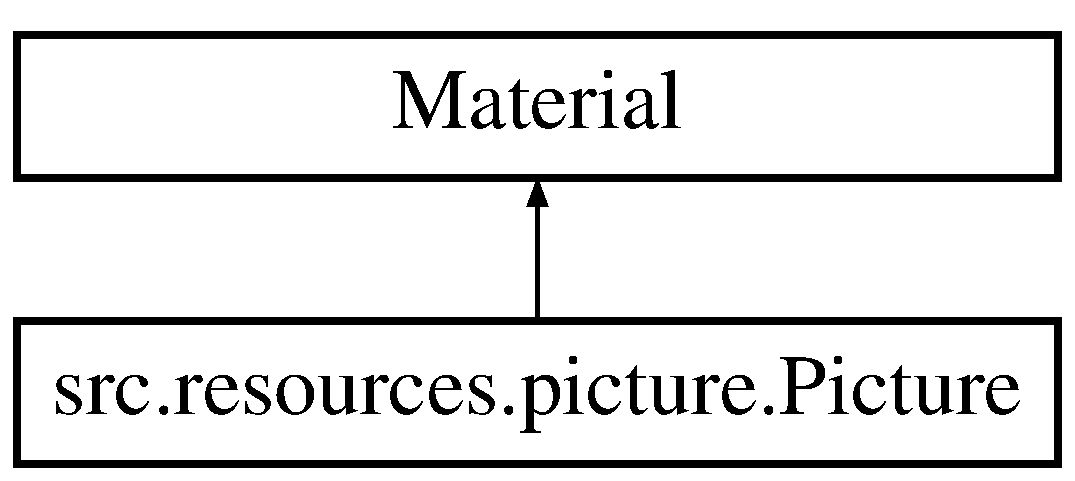
\includegraphics[height=2.000000cm]{classsrc_1_1resources_1_1picture_1_1_picture}
\end{center}
\end{figure}
\subsection*{Public Member Functions}
\begin{DoxyCompactItemize}
\item 
def \hyperlink{classsrc_1_1resources_1_1picture_1_1_picture_adc6ea066102180580a8183fd9c8d6d09}{\+\_\+\+\_\+init\+\_\+\+\_\+}
\end{DoxyCompactItemize}
\subsection*{Public Attributes}
\begin{DoxyCompactItemize}
\item 
\hyperlink{classsrc_1_1resources_1_1picture_1_1_picture_a003b41ddc2d0551e5f8271eea1563f88}{filename}
\item 
\hyperlink{classsrc_1_1resources_1_1picture_1_1_picture_a3eac2bc1d9a3bc1f85b441e16719a4b7}{reference}
\item 
\hyperlink{classsrc_1_1resources_1_1picture_1_1_picture_ad9329b3048acfd8dacef0dfe9ca57ded}{width}
\item 
\hyperlink{classsrc_1_1resources_1_1picture_1_1_picture_a7648bd554fb274458f7cc32fa7c48e4a}{height}
\item 
\hyperlink{classsrc_1_1resources_1_1picture_1_1_picture_afce02889d8db77869eee3103da6c46f5}{format}
\end{DoxyCompactItemize}


\subsection{Detailed Description}


Definition at line 5 of file picture.\+py.



\subsection{Constructor \& Destructor Documentation}
\hypertarget{classsrc_1_1resources_1_1picture_1_1_picture_adc6ea066102180580a8183fd9c8d6d09}{\index{src\+::resources\+::picture\+::\+Picture@{src\+::resources\+::picture\+::\+Picture}!\+\_\+\+\_\+init\+\_\+\+\_\+@{\+\_\+\+\_\+init\+\_\+\+\_\+}}
\index{\+\_\+\+\_\+init\+\_\+\+\_\+@{\+\_\+\+\_\+init\+\_\+\+\_\+}!src\+::resources\+::picture\+::\+Picture@{src\+::resources\+::picture\+::\+Picture}}
\subsubsection[{\+\_\+\+\_\+init\+\_\+\+\_\+}]{\setlength{\rightskip}{0pt plus 5cm}def src.\+resources.\+picture.\+Picture.\+\_\+\+\_\+init\+\_\+\+\_\+ (
\begin{DoxyParamCaption}
\item[{}]{self}
\end{DoxyParamCaption}
)}}\label{classsrc_1_1resources_1_1picture_1_1_picture_adc6ea066102180580a8183fd9c8d6d09}


Definition at line 6 of file picture.\+py.



\subsection{Member Data Documentation}
\hypertarget{classsrc_1_1resources_1_1picture_1_1_picture_a003b41ddc2d0551e5f8271eea1563f88}{\index{src\+::resources\+::picture\+::\+Picture@{src\+::resources\+::picture\+::\+Picture}!filename@{filename}}
\index{filename@{filename}!src\+::resources\+::picture\+::\+Picture@{src\+::resources\+::picture\+::\+Picture}}
\subsubsection[{filename}]{\setlength{\rightskip}{0pt plus 5cm}src.\+resources.\+picture.\+Picture.\+filename}}\label{classsrc_1_1resources_1_1picture_1_1_picture_a003b41ddc2d0551e5f8271eea1563f88}


Definition at line 7 of file picture.\+py.

\hypertarget{classsrc_1_1resources_1_1picture_1_1_picture_afce02889d8db77869eee3103da6c46f5}{\index{src\+::resources\+::picture\+::\+Picture@{src\+::resources\+::picture\+::\+Picture}!format@{format}}
\index{format@{format}!src\+::resources\+::picture\+::\+Picture@{src\+::resources\+::picture\+::\+Picture}}
\subsubsection[{format}]{\setlength{\rightskip}{0pt plus 5cm}src.\+resources.\+picture.\+Picture.\+format}}\label{classsrc_1_1resources_1_1picture_1_1_picture_afce02889d8db77869eee3103da6c46f5}


Definition at line 11 of file picture.\+py.

\hypertarget{classsrc_1_1resources_1_1picture_1_1_picture_a7648bd554fb274458f7cc32fa7c48e4a}{\index{src\+::resources\+::picture\+::\+Picture@{src\+::resources\+::picture\+::\+Picture}!height@{height}}
\index{height@{height}!src\+::resources\+::picture\+::\+Picture@{src\+::resources\+::picture\+::\+Picture}}
\subsubsection[{height}]{\setlength{\rightskip}{0pt plus 5cm}src.\+resources.\+picture.\+Picture.\+height}}\label{classsrc_1_1resources_1_1picture_1_1_picture_a7648bd554fb274458f7cc32fa7c48e4a}


Definition at line 10 of file picture.\+py.

\hypertarget{classsrc_1_1resources_1_1picture_1_1_picture_a3eac2bc1d9a3bc1f85b441e16719a4b7}{\index{src\+::resources\+::picture\+::\+Picture@{src\+::resources\+::picture\+::\+Picture}!reference@{reference}}
\index{reference@{reference}!src\+::resources\+::picture\+::\+Picture@{src\+::resources\+::picture\+::\+Picture}}
\subsubsection[{reference}]{\setlength{\rightskip}{0pt plus 5cm}src.\+resources.\+picture.\+Picture.\+reference}}\label{classsrc_1_1resources_1_1picture_1_1_picture_a3eac2bc1d9a3bc1f85b441e16719a4b7}


Definition at line 8 of file picture.\+py.

\hypertarget{classsrc_1_1resources_1_1picture_1_1_picture_ad9329b3048acfd8dacef0dfe9ca57ded}{\index{src\+::resources\+::picture\+::\+Picture@{src\+::resources\+::picture\+::\+Picture}!width@{width}}
\index{width@{width}!src\+::resources\+::picture\+::\+Picture@{src\+::resources\+::picture\+::\+Picture}}
\subsubsection[{width}]{\setlength{\rightskip}{0pt plus 5cm}src.\+resources.\+picture.\+Picture.\+width}}\label{classsrc_1_1resources_1_1picture_1_1_picture_ad9329b3048acfd8dacef0dfe9ca57ded}


Definition at line 9 of file picture.\+py.



The documentation for this class was generated from the following file\+:\begin{DoxyCompactItemize}
\item 
/\+Users/celine/\+Work/\+C\+N\+R\+S/workspace/\+Himal\+Co/dev/lib/lmf/src/resources/\hyperlink{picture_8py}{picture.\+py}\end{DoxyCompactItemize}

\hypertarget{classsrc_1_1morphology_1_1related__form_1_1_related_form}{\section{src.\+morphology.\+related\+\_\+form.\+Related\+Form Class Reference}
\label{classsrc_1_1morphology_1_1related__form_1_1_related_form}\index{src.\+morphology.\+related\+\_\+form.\+Related\+Form@{src.\+morphology.\+related\+\_\+form.\+Related\+Form}}
}
Inheritance diagram for src.\+morphology.\+related\+\_\+form.\+Related\+Form\+:\begin{figure}[H]
\begin{center}
\leavevmode
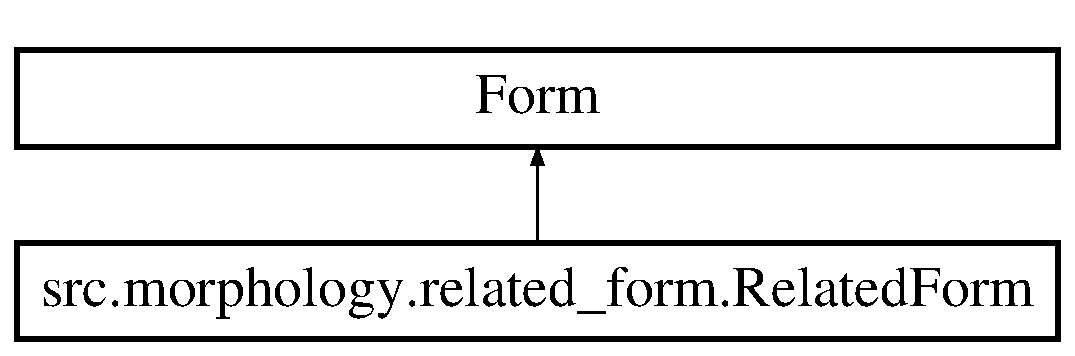
\includegraphics[height=2.000000cm]{classsrc_1_1morphology_1_1related__form_1_1_related_form}
\end{center}
\end{figure}
\subsection*{Public Member Functions}
\begin{DoxyCompactItemize}
\item 
def \hyperlink{classsrc_1_1morphology_1_1related__form_1_1_related_form_abdb8f278733f3a984fd77232c417fde4}{\+\_\+\+\_\+init\+\_\+\+\_\+}
\end{DoxyCompactItemize}
\subsection*{Public Attributes}
\begin{DoxyCompactItemize}
\item 
\hyperlink{classsrc_1_1morphology_1_1related__form_1_1_related_form_a266c933a3387b83a172bc18bb1bcc556}{semantic\+Relation}
\end{DoxyCompactItemize}


\subsection{Detailed Description}


Definition at line 5 of file related\+\_\+form.\+py.



\subsection{Constructor \& Destructor Documentation}
\hypertarget{classsrc_1_1morphology_1_1related__form_1_1_related_form_abdb8f278733f3a984fd77232c417fde4}{\index{src\+::morphology\+::related\+\_\+form\+::\+Related\+Form@{src\+::morphology\+::related\+\_\+form\+::\+Related\+Form}!\+\_\+\+\_\+init\+\_\+\+\_\+@{\+\_\+\+\_\+init\+\_\+\+\_\+}}
\index{\+\_\+\+\_\+init\+\_\+\+\_\+@{\+\_\+\+\_\+init\+\_\+\+\_\+}!src\+::morphology\+::related\+\_\+form\+::\+Related\+Form@{src\+::morphology\+::related\+\_\+form\+::\+Related\+Form}}
\subsubsection[{\+\_\+\+\_\+init\+\_\+\+\_\+}]{\setlength{\rightskip}{0pt plus 5cm}def src.\+morphology.\+related\+\_\+form.\+Related\+Form.\+\_\+\+\_\+init\+\_\+\+\_\+ (
\begin{DoxyParamCaption}
\item[{}]{self}
\end{DoxyParamCaption}
)}}\label{classsrc_1_1morphology_1_1related__form_1_1_related_form_abdb8f278733f3a984fd77232c417fde4}


Definition at line 6 of file related\+\_\+form.\+py.



\subsection{Member Data Documentation}
\hypertarget{classsrc_1_1morphology_1_1related__form_1_1_related_form_a266c933a3387b83a172bc18bb1bcc556}{\index{src\+::morphology\+::related\+\_\+form\+::\+Related\+Form@{src\+::morphology\+::related\+\_\+form\+::\+Related\+Form}!semantic\+Relation@{semantic\+Relation}}
\index{semantic\+Relation@{semantic\+Relation}!src\+::morphology\+::related\+\_\+form\+::\+Related\+Form@{src\+::morphology\+::related\+\_\+form\+::\+Related\+Form}}
\subsubsection[{semantic\+Relation}]{\setlength{\rightskip}{0pt plus 5cm}src.\+morphology.\+related\+\_\+form.\+Related\+Form.\+semantic\+Relation}}\label{classsrc_1_1morphology_1_1related__form_1_1_related_form_a266c933a3387b83a172bc18bb1bcc556}


Definition at line 7 of file related\+\_\+form.\+py.



The documentation for this class was generated from the following file\+:\begin{DoxyCompactItemize}
\item 
/\+Users/celine/\+Work/\+C\+N\+R\+S/workspace/\+Himal\+Co/dev/lib/lmf/src/morphology/\hyperlink{related__form_8py}{related\+\_\+form.\+py}\end{DoxyCompactItemize}

\hypertarget{classsrc_1_1core_1_1representation_1_1_representation}{\section{src.\+core.\+representation.\+Representation Class Reference}
\label{classsrc_1_1core_1_1representation_1_1_representation}\index{src.\+core.\+representation.\+Representation@{src.\+core.\+representation.\+Representation}}
}
\subsection*{Public Member Functions}
\begin{DoxyCompactItemize}
\item 
def \hyperlink{classsrc_1_1core_1_1representation_1_1_representation_ac2a2d057963db31cf13f93cee36c8c64}{\+\_\+\+\_\+init\+\_\+\+\_\+}
\end{DoxyCompactItemize}
\subsection*{Public Attributes}
\begin{DoxyCompactItemize}
\item 
\hyperlink{classsrc_1_1core_1_1representation_1_1_representation_a72e49f86ec58c698f2a75c2046d25d62}{comment}
\item 
\hyperlink{classsrc_1_1core_1_1representation_1_1_representation_ad4ec4b05057384573370ea9513f16a8f}{written\+Form}
\item 
\hyperlink{classsrc_1_1core_1_1representation_1_1_representation_a01443961d9cdedf9d6353d9a140644d6}{language}
\end{DoxyCompactItemize}


\subsection{Detailed Description}


Definition at line 3 of file representation.\+py.



\subsection{Constructor \& Destructor Documentation}
\hypertarget{classsrc_1_1core_1_1representation_1_1_representation_ac2a2d057963db31cf13f93cee36c8c64}{\index{src\+::core\+::representation\+::\+Representation@{src\+::core\+::representation\+::\+Representation}!\+\_\+\+\_\+init\+\_\+\+\_\+@{\+\_\+\+\_\+init\+\_\+\+\_\+}}
\index{\+\_\+\+\_\+init\+\_\+\+\_\+@{\+\_\+\+\_\+init\+\_\+\+\_\+}!src\+::core\+::representation\+::\+Representation@{src\+::core\+::representation\+::\+Representation}}
\subsubsection[{\+\_\+\+\_\+init\+\_\+\+\_\+}]{\setlength{\rightskip}{0pt plus 5cm}def src.\+core.\+representation.\+Representation.\+\_\+\+\_\+init\+\_\+\+\_\+ (
\begin{DoxyParamCaption}
\item[{}]{self}
\end{DoxyParamCaption}
)}}\label{classsrc_1_1core_1_1representation_1_1_representation_ac2a2d057963db31cf13f93cee36c8c64}


Definition at line 4 of file representation.\+py.



\subsection{Member Data Documentation}
\hypertarget{classsrc_1_1core_1_1representation_1_1_representation_a72e49f86ec58c698f2a75c2046d25d62}{\index{src\+::core\+::representation\+::\+Representation@{src\+::core\+::representation\+::\+Representation}!comment@{comment}}
\index{comment@{comment}!src\+::core\+::representation\+::\+Representation@{src\+::core\+::representation\+::\+Representation}}
\subsubsection[{comment}]{\setlength{\rightskip}{0pt plus 5cm}src.\+core.\+representation.\+Representation.\+comment}}\label{classsrc_1_1core_1_1representation_1_1_representation_a72e49f86ec58c698f2a75c2046d25d62}


Definition at line 5 of file representation.\+py.

\hypertarget{classsrc_1_1core_1_1representation_1_1_representation_a01443961d9cdedf9d6353d9a140644d6}{\index{src\+::core\+::representation\+::\+Representation@{src\+::core\+::representation\+::\+Representation}!language@{language}}
\index{language@{language}!src\+::core\+::representation\+::\+Representation@{src\+::core\+::representation\+::\+Representation}}
\subsubsection[{language}]{\setlength{\rightskip}{0pt plus 5cm}src.\+core.\+representation.\+Representation.\+language}}\label{classsrc_1_1core_1_1representation_1_1_representation_a01443961d9cdedf9d6353d9a140644d6}


Definition at line 7 of file representation.\+py.

\hypertarget{classsrc_1_1core_1_1representation_1_1_representation_ad4ec4b05057384573370ea9513f16a8f}{\index{src\+::core\+::representation\+::\+Representation@{src\+::core\+::representation\+::\+Representation}!written\+Form@{written\+Form}}
\index{written\+Form@{written\+Form}!src\+::core\+::representation\+::\+Representation@{src\+::core\+::representation\+::\+Representation}}
\subsubsection[{written\+Form}]{\setlength{\rightskip}{0pt plus 5cm}src.\+core.\+representation.\+Representation.\+written\+Form}}\label{classsrc_1_1core_1_1representation_1_1_representation_ad4ec4b05057384573370ea9513f16a8f}


Definition at line 6 of file representation.\+py.



The documentation for this class was generated from the following file\+:\begin{DoxyCompactItemize}
\item 
/\+Users/celine/\+Work/\+C\+N\+R\+S/workspace/\+Himal\+Co/dev/lib/lmf/src/core/\hyperlink{representation_8py}{representation.\+py}\end{DoxyCompactItemize}

\hypertarget{classsrc_1_1resources_1_1resource_1_1_resource}{\section{src.\+resources.\+resource.\+Resource Class Reference}
\label{classsrc_1_1resources_1_1resource_1_1_resource}\index{src.\+resources.\+resource.\+Resource@{src.\+resources.\+resource.\+Resource}}
}
\subsection*{Public Member Functions}
\begin{DoxyCompactItemize}
\item 
def \hyperlink{classsrc_1_1resources_1_1resource_1_1_resource_ab121b71dde3799e39bc6de236263279f}{\+\_\+\+\_\+init\+\_\+\+\_\+}
\end{DoxyCompactItemize}


\subsection{Detailed Description}


Definition at line 3 of file resource.\+py.



\subsection{Constructor \& Destructor Documentation}
\hypertarget{classsrc_1_1resources_1_1resource_1_1_resource_ab121b71dde3799e39bc6de236263279f}{\index{src\+::resources\+::resource\+::\+Resource@{src\+::resources\+::resource\+::\+Resource}!\+\_\+\+\_\+init\+\_\+\+\_\+@{\+\_\+\+\_\+init\+\_\+\+\_\+}}
\index{\+\_\+\+\_\+init\+\_\+\+\_\+@{\+\_\+\+\_\+init\+\_\+\+\_\+}!src\+::resources\+::resource\+::\+Resource@{src\+::resources\+::resource\+::\+Resource}}
\subsubsection[{\+\_\+\+\_\+init\+\_\+\+\_\+}]{\setlength{\rightskip}{0pt plus 5cm}def src.\+resources.\+resource.\+Resource.\+\_\+\+\_\+init\+\_\+\+\_\+ (
\begin{DoxyParamCaption}
\item[{}]{self}
\end{DoxyParamCaption}
)}}\label{classsrc_1_1resources_1_1resource_1_1_resource_ab121b71dde3799e39bc6de236263279f}


Definition at line 4 of file resource.\+py.



The documentation for this class was generated from the following file\+:\begin{DoxyCompactItemize}
\item 
/\+Users/celine/\+Work/\+C\+N\+R\+S/workspace/\+Himal\+Co/dev/lib/lmf/src/resources/\hyperlink{resource_8py}{resource.\+py}\end{DoxyCompactItemize}

\hypertarget{classsrc_1_1core_1_1sense_1_1_sense}{\section{src.\+core.\+sense.\+Sense Class Reference}
\label{classsrc_1_1core_1_1sense_1_1_sense}\index{src.\+core.\+sense.\+Sense@{src.\+core.\+sense.\+Sense}}
}
\subsection*{Public Member Functions}
\begin{DoxyCompactItemize}
\item 
def \hyperlink{classsrc_1_1core_1_1sense_1_1_sense_a006b5ecf12a85db68f7bab5af6fed6c3}{\+\_\+\+\_\+init\+\_\+\+\_\+}
\end{DoxyCompactItemize}
\subsection*{Public Attributes}
\begin{DoxyCompactItemize}
\item 
\hyperlink{classsrc_1_1core_1_1sense_1_1_sense_acfebe4764025fd6062674315e2c4230f}{sense\+Number}
\item 
\hyperlink{classsrc_1_1core_1_1sense_1_1_sense_a37a8c62a8fbdbc3191b25b2654197307}{id}
\end{DoxyCompactItemize}


\subsection{Detailed Description}


Definition at line 3 of file sense.\+py.



\subsection{Constructor \& Destructor Documentation}
\hypertarget{classsrc_1_1core_1_1sense_1_1_sense_a006b5ecf12a85db68f7bab5af6fed6c3}{\index{src\+::core\+::sense\+::\+Sense@{src\+::core\+::sense\+::\+Sense}!\+\_\+\+\_\+init\+\_\+\+\_\+@{\+\_\+\+\_\+init\+\_\+\+\_\+}}
\index{\+\_\+\+\_\+init\+\_\+\+\_\+@{\+\_\+\+\_\+init\+\_\+\+\_\+}!src\+::core\+::sense\+::\+Sense@{src\+::core\+::sense\+::\+Sense}}
\subsubsection[{\+\_\+\+\_\+init\+\_\+\+\_\+}]{\setlength{\rightskip}{0pt plus 5cm}def src.\+core.\+sense.\+Sense.\+\_\+\+\_\+init\+\_\+\+\_\+ (
\begin{DoxyParamCaption}
\item[{}]{self}
\end{DoxyParamCaption}
)}}\label{classsrc_1_1core_1_1sense_1_1_sense_a006b5ecf12a85db68f7bab5af6fed6c3}


Definition at line 4 of file sense.\+py.



\subsection{Member Data Documentation}
\hypertarget{classsrc_1_1core_1_1sense_1_1_sense_a37a8c62a8fbdbc3191b25b2654197307}{\index{src\+::core\+::sense\+::\+Sense@{src\+::core\+::sense\+::\+Sense}!id@{id}}
\index{id@{id}!src\+::core\+::sense\+::\+Sense@{src\+::core\+::sense\+::\+Sense}}
\subsubsection[{id}]{\setlength{\rightskip}{0pt plus 5cm}src.\+core.\+sense.\+Sense.\+id}}\label{classsrc_1_1core_1_1sense_1_1_sense_a37a8c62a8fbdbc3191b25b2654197307}


Definition at line 6 of file sense.\+py.

\hypertarget{classsrc_1_1core_1_1sense_1_1_sense_acfebe4764025fd6062674315e2c4230f}{\index{src\+::core\+::sense\+::\+Sense@{src\+::core\+::sense\+::\+Sense}!sense\+Number@{sense\+Number}}
\index{sense\+Number@{sense\+Number}!src\+::core\+::sense\+::\+Sense@{src\+::core\+::sense\+::\+Sense}}
\subsubsection[{sense\+Number}]{\setlength{\rightskip}{0pt plus 5cm}src.\+core.\+sense.\+Sense.\+sense\+Number}}\label{classsrc_1_1core_1_1sense_1_1_sense_acfebe4764025fd6062674315e2c4230f}


Definition at line 5 of file sense.\+py.



The documentation for this class was generated from the following file\+:\begin{DoxyCompactItemize}
\item 
/\+Users/celine/\+Work/\+C\+N\+R\+S/workspace/\+Himal\+Co/dev/lib/lmf/src/core/\hyperlink{sense_8py}{sense.\+py}\end{DoxyCompactItemize}

\hypertarget{classsrc_1_1resources_1_1speaker_1_1_speaker}{\section{src.\+resources.\+speaker.\+Speaker Class Reference}
\label{classsrc_1_1resources_1_1speaker_1_1_speaker}\index{src.\+resources.\+speaker.\+Speaker@{src.\+resources.\+speaker.\+Speaker}}
}
Inheritance diagram for src.\+resources.\+speaker.\+Speaker\+:\begin{figure}[H]
\begin{center}
\leavevmode
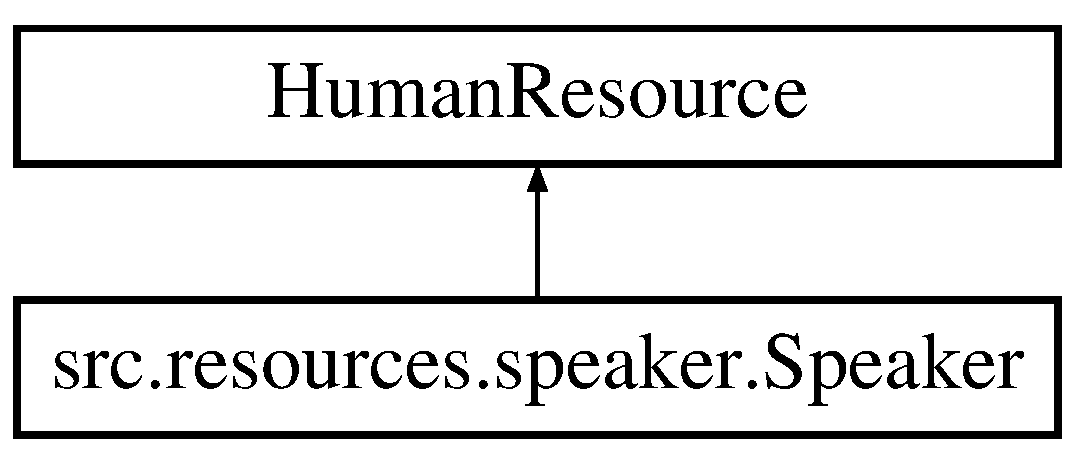
\includegraphics[height=2.000000cm]{classsrc_1_1resources_1_1speaker_1_1_speaker}
\end{center}
\end{figure}
\subsection*{Public Member Functions}
\begin{DoxyCompactItemize}
\item 
def \hyperlink{classsrc_1_1resources_1_1speaker_1_1_speaker_a019f0817887d4145fc13f4696a4f8baa}{\+\_\+\+\_\+init\+\_\+\+\_\+}
\end{DoxyCompactItemize}
\subsection*{Public Attributes}
\begin{DoxyCompactItemize}
\item 
\hyperlink{classsrc_1_1resources_1_1speaker_1_1_speaker_abe55b033660bc93fd7400f01a996a2dc}{speaker\+I\+D}
\end{DoxyCompactItemize}


\subsection{Detailed Description}


Definition at line 5 of file speaker.\+py.



\subsection{Constructor \& Destructor Documentation}
\hypertarget{classsrc_1_1resources_1_1speaker_1_1_speaker_a019f0817887d4145fc13f4696a4f8baa}{\index{src\+::resources\+::speaker\+::\+Speaker@{src\+::resources\+::speaker\+::\+Speaker}!\+\_\+\+\_\+init\+\_\+\+\_\+@{\+\_\+\+\_\+init\+\_\+\+\_\+}}
\index{\+\_\+\+\_\+init\+\_\+\+\_\+@{\+\_\+\+\_\+init\+\_\+\+\_\+}!src\+::resources\+::speaker\+::\+Speaker@{src\+::resources\+::speaker\+::\+Speaker}}
\subsubsection[{\+\_\+\+\_\+init\+\_\+\+\_\+}]{\setlength{\rightskip}{0pt plus 5cm}def src.\+resources.\+speaker.\+Speaker.\+\_\+\+\_\+init\+\_\+\+\_\+ (
\begin{DoxyParamCaption}
\item[{}]{self}
\end{DoxyParamCaption}
)}}\label{classsrc_1_1resources_1_1speaker_1_1_speaker_a019f0817887d4145fc13f4696a4f8baa}


Definition at line 6 of file speaker.\+py.



\subsection{Member Data Documentation}
\hypertarget{classsrc_1_1resources_1_1speaker_1_1_speaker_abe55b033660bc93fd7400f01a996a2dc}{\index{src\+::resources\+::speaker\+::\+Speaker@{src\+::resources\+::speaker\+::\+Speaker}!speaker\+I\+D@{speaker\+I\+D}}
\index{speaker\+I\+D@{speaker\+I\+D}!src\+::resources\+::speaker\+::\+Speaker@{src\+::resources\+::speaker\+::\+Speaker}}
\subsubsection[{speaker\+I\+D}]{\setlength{\rightskip}{0pt plus 5cm}src.\+resources.\+speaker.\+Speaker.\+speaker\+I\+D}}\label{classsrc_1_1resources_1_1speaker_1_1_speaker_abe55b033660bc93fd7400f01a996a2dc}


Definition at line 7 of file speaker.\+py.



The documentation for this class was generated from the following file\+:\begin{DoxyCompactItemize}
\item 
/\+Users/celine/\+Work/\+C\+N\+R\+S/workspace/\+Himal\+Co/dev/lib/lmf/src/resources/\hyperlink{speaker_8py}{speaker.\+py}\end{DoxyCompactItemize}

\hypertarget{classsrc_1_1core_1_1statement_1_1_statement}{\section{src.\+core.\+statement.\+Statement Class Reference}
\label{classsrc_1_1core_1_1statement_1_1_statement}\index{src.\+core.\+statement.\+Statement@{src.\+core.\+statement.\+Statement}}
}
\subsection*{Public Member Functions}
\begin{DoxyCompactItemize}
\item 
def \hyperlink{classsrc_1_1core_1_1statement_1_1_statement_abf2bda0e5f09d1f483ce7ab7d1eb9909}{\+\_\+\+\_\+init\+\_\+\+\_\+}
\end{DoxyCompactItemize}
\subsection*{Public Attributes}
\begin{DoxyCompactItemize}
\item 
\hyperlink{classsrc_1_1core_1_1statement_1_1_statement_a2cbc454e31333b14ed7f894df8af2fce}{note\+Type}
\item 
\hyperlink{classsrc_1_1core_1_1statement_1_1_statement_a2edc72dff8f04376c6f09fc9a270503b}{note}
\item 
\hyperlink{classsrc_1_1core_1_1statement_1_1_statement_a62916eea6e03f2115544f9fd6d8042fc}{language}
\item 
\hyperlink{classsrc_1_1core_1_1statement_1_1_statement_ac27bf20184c2fe3fc081af160a34b078}{encyclopedic\+Information}
\item 
\hyperlink{classsrc_1_1core_1_1statement_1_1_statement_afbcca36f7315bd8b556f31a6c73da2e8}{usage\+Note}
\item 
\hyperlink{classsrc_1_1core_1_1statement_1_1_statement_a95cc64760bb64c330e5dc921c00981c9}{restriction}
\item 
\hyperlink{classsrc_1_1core_1_1statement_1_1_statement_a43c11e8a1f1b8dcf1c47138630ce9014}{derivation}
\item 
\hyperlink{classsrc_1_1core_1_1statement_1_1_statement_ad335aefcefa9ae166c0cae1e553e2bf3}{borrowed\+Word}
\item 
\hyperlink{classsrc_1_1core_1_1statement_1_1_statement_a754fb4718f6f6a7999094cedb98716cb}{written\+Form}
\item 
\hyperlink{classsrc_1_1core_1_1statement_1_1_statement_aae184efd75880bebe51b7c8161ce0e81}{sense}
\item 
\hyperlink{classsrc_1_1core_1_1statement_1_1_statement_a39257f2e47ab775116eae335c871f30d}{etymology}
\item 
\hyperlink{classsrc_1_1core_1_1statement_1_1_statement_a75153a36438fe45f7b4c6da80dc2eb5b}{etymology\+Comment}
\item 
\hyperlink{classsrc_1_1core_1_1statement_1_1_statement_ac5b1ca26900e8f0d6407658195820157}{etymology\+Gloss}
\item 
\hyperlink{classsrc_1_1core_1_1statement_1_1_statement_afb34d7f04ad71ed5a0fe62932305f743}{etymology\+Source}
\item 
\hyperlink{classsrc_1_1core_1_1statement_1_1_statement_ab1bd16d721a81ebae7f1e0fb5da23d0f}{term\+Source\+Language}
\item 
\hyperlink{classsrc_1_1core_1_1statement_1_1_statement_a8ff06170be6b1b8856c0b2c78c458dac}{target\+Lexical\+Entry}
\item 
\hyperlink{classsrc_1_1core_1_1statement_1_1_statement_addc80054a840f2859f503389e53a247c}{scientific\+Name}
\end{DoxyCompactItemize}


\subsection{Detailed Description}


Definition at line 3 of file statement.\+py.



\subsection{Constructor \& Destructor Documentation}
\hypertarget{classsrc_1_1core_1_1statement_1_1_statement_abf2bda0e5f09d1f483ce7ab7d1eb9909}{\index{src\+::core\+::statement\+::\+Statement@{src\+::core\+::statement\+::\+Statement}!\+\_\+\+\_\+init\+\_\+\+\_\+@{\+\_\+\+\_\+init\+\_\+\+\_\+}}
\index{\+\_\+\+\_\+init\+\_\+\+\_\+@{\+\_\+\+\_\+init\+\_\+\+\_\+}!src\+::core\+::statement\+::\+Statement@{src\+::core\+::statement\+::\+Statement}}
\subsubsection[{\+\_\+\+\_\+init\+\_\+\+\_\+}]{\setlength{\rightskip}{0pt plus 5cm}def src.\+core.\+statement.\+Statement.\+\_\+\+\_\+init\+\_\+\+\_\+ (
\begin{DoxyParamCaption}
\item[{}]{self}
\end{DoxyParamCaption}
)}}\label{classsrc_1_1core_1_1statement_1_1_statement_abf2bda0e5f09d1f483ce7ab7d1eb9909}


Definition at line 4 of file statement.\+py.



\subsection{Member Data Documentation}
\hypertarget{classsrc_1_1core_1_1statement_1_1_statement_ad335aefcefa9ae166c0cae1e553e2bf3}{\index{src\+::core\+::statement\+::\+Statement@{src\+::core\+::statement\+::\+Statement}!borrowed\+Word@{borrowed\+Word}}
\index{borrowed\+Word@{borrowed\+Word}!src\+::core\+::statement\+::\+Statement@{src\+::core\+::statement\+::\+Statement}}
\subsubsection[{borrowed\+Word}]{\setlength{\rightskip}{0pt plus 5cm}src.\+core.\+statement.\+Statement.\+borrowed\+Word}}\label{classsrc_1_1core_1_1statement_1_1_statement_ad335aefcefa9ae166c0cae1e553e2bf3}


Definition at line 12 of file statement.\+py.

\hypertarget{classsrc_1_1core_1_1statement_1_1_statement_a43c11e8a1f1b8dcf1c47138630ce9014}{\index{src\+::core\+::statement\+::\+Statement@{src\+::core\+::statement\+::\+Statement}!derivation@{derivation}}
\index{derivation@{derivation}!src\+::core\+::statement\+::\+Statement@{src\+::core\+::statement\+::\+Statement}}
\subsubsection[{derivation}]{\setlength{\rightskip}{0pt plus 5cm}src.\+core.\+statement.\+Statement.\+derivation}}\label{classsrc_1_1core_1_1statement_1_1_statement_a43c11e8a1f1b8dcf1c47138630ce9014}


Definition at line 11 of file statement.\+py.

\hypertarget{classsrc_1_1core_1_1statement_1_1_statement_ac27bf20184c2fe3fc081af160a34b078}{\index{src\+::core\+::statement\+::\+Statement@{src\+::core\+::statement\+::\+Statement}!encyclopedic\+Information@{encyclopedic\+Information}}
\index{encyclopedic\+Information@{encyclopedic\+Information}!src\+::core\+::statement\+::\+Statement@{src\+::core\+::statement\+::\+Statement}}
\subsubsection[{encyclopedic\+Information}]{\setlength{\rightskip}{0pt plus 5cm}src.\+core.\+statement.\+Statement.\+encyclopedic\+Information}}\label{classsrc_1_1core_1_1statement_1_1_statement_ac27bf20184c2fe3fc081af160a34b078}


Definition at line 8 of file statement.\+py.

\hypertarget{classsrc_1_1core_1_1statement_1_1_statement_a39257f2e47ab775116eae335c871f30d}{\index{src\+::core\+::statement\+::\+Statement@{src\+::core\+::statement\+::\+Statement}!etymology@{etymology}}
\index{etymology@{etymology}!src\+::core\+::statement\+::\+Statement@{src\+::core\+::statement\+::\+Statement}}
\subsubsection[{etymology}]{\setlength{\rightskip}{0pt plus 5cm}src.\+core.\+statement.\+Statement.\+etymology}}\label{classsrc_1_1core_1_1statement_1_1_statement_a39257f2e47ab775116eae335c871f30d}


Definition at line 15 of file statement.\+py.

\hypertarget{classsrc_1_1core_1_1statement_1_1_statement_a75153a36438fe45f7b4c6da80dc2eb5b}{\index{src\+::core\+::statement\+::\+Statement@{src\+::core\+::statement\+::\+Statement}!etymology\+Comment@{etymology\+Comment}}
\index{etymology\+Comment@{etymology\+Comment}!src\+::core\+::statement\+::\+Statement@{src\+::core\+::statement\+::\+Statement}}
\subsubsection[{etymology\+Comment}]{\setlength{\rightskip}{0pt plus 5cm}src.\+core.\+statement.\+Statement.\+etymology\+Comment}}\label{classsrc_1_1core_1_1statement_1_1_statement_a75153a36438fe45f7b4c6da80dc2eb5b}


Definition at line 16 of file statement.\+py.

\hypertarget{classsrc_1_1core_1_1statement_1_1_statement_ac5b1ca26900e8f0d6407658195820157}{\index{src\+::core\+::statement\+::\+Statement@{src\+::core\+::statement\+::\+Statement}!etymology\+Gloss@{etymology\+Gloss}}
\index{etymology\+Gloss@{etymology\+Gloss}!src\+::core\+::statement\+::\+Statement@{src\+::core\+::statement\+::\+Statement}}
\subsubsection[{etymology\+Gloss}]{\setlength{\rightskip}{0pt plus 5cm}src.\+core.\+statement.\+Statement.\+etymology\+Gloss}}\label{classsrc_1_1core_1_1statement_1_1_statement_ac5b1ca26900e8f0d6407658195820157}


Definition at line 17 of file statement.\+py.

\hypertarget{classsrc_1_1core_1_1statement_1_1_statement_afb34d7f04ad71ed5a0fe62932305f743}{\index{src\+::core\+::statement\+::\+Statement@{src\+::core\+::statement\+::\+Statement}!etymology\+Source@{etymology\+Source}}
\index{etymology\+Source@{etymology\+Source}!src\+::core\+::statement\+::\+Statement@{src\+::core\+::statement\+::\+Statement}}
\subsubsection[{etymology\+Source}]{\setlength{\rightskip}{0pt plus 5cm}src.\+core.\+statement.\+Statement.\+etymology\+Source}}\label{classsrc_1_1core_1_1statement_1_1_statement_afb34d7f04ad71ed5a0fe62932305f743}


Definition at line 18 of file statement.\+py.

\hypertarget{classsrc_1_1core_1_1statement_1_1_statement_a62916eea6e03f2115544f9fd6d8042fc}{\index{src\+::core\+::statement\+::\+Statement@{src\+::core\+::statement\+::\+Statement}!language@{language}}
\index{language@{language}!src\+::core\+::statement\+::\+Statement@{src\+::core\+::statement\+::\+Statement}}
\subsubsection[{language}]{\setlength{\rightskip}{0pt plus 5cm}src.\+core.\+statement.\+Statement.\+language}}\label{classsrc_1_1core_1_1statement_1_1_statement_a62916eea6e03f2115544f9fd6d8042fc}


Definition at line 7 of file statement.\+py.

\hypertarget{classsrc_1_1core_1_1statement_1_1_statement_a2edc72dff8f04376c6f09fc9a270503b}{\index{src\+::core\+::statement\+::\+Statement@{src\+::core\+::statement\+::\+Statement}!note@{note}}
\index{note@{note}!src\+::core\+::statement\+::\+Statement@{src\+::core\+::statement\+::\+Statement}}
\subsubsection[{note}]{\setlength{\rightskip}{0pt plus 5cm}src.\+core.\+statement.\+Statement.\+note}}\label{classsrc_1_1core_1_1statement_1_1_statement_a2edc72dff8f04376c6f09fc9a270503b}


Definition at line 6 of file statement.\+py.

\hypertarget{classsrc_1_1core_1_1statement_1_1_statement_a2cbc454e31333b14ed7f894df8af2fce}{\index{src\+::core\+::statement\+::\+Statement@{src\+::core\+::statement\+::\+Statement}!note\+Type@{note\+Type}}
\index{note\+Type@{note\+Type}!src\+::core\+::statement\+::\+Statement@{src\+::core\+::statement\+::\+Statement}}
\subsubsection[{note\+Type}]{\setlength{\rightskip}{0pt plus 5cm}src.\+core.\+statement.\+Statement.\+note\+Type}}\label{classsrc_1_1core_1_1statement_1_1_statement_a2cbc454e31333b14ed7f894df8af2fce}


Definition at line 5 of file statement.\+py.

\hypertarget{classsrc_1_1core_1_1statement_1_1_statement_a95cc64760bb64c330e5dc921c00981c9}{\index{src\+::core\+::statement\+::\+Statement@{src\+::core\+::statement\+::\+Statement}!restriction@{restriction}}
\index{restriction@{restriction}!src\+::core\+::statement\+::\+Statement@{src\+::core\+::statement\+::\+Statement}}
\subsubsection[{restriction}]{\setlength{\rightskip}{0pt plus 5cm}src.\+core.\+statement.\+Statement.\+restriction}}\label{classsrc_1_1core_1_1statement_1_1_statement_a95cc64760bb64c330e5dc921c00981c9}


Definition at line 10 of file statement.\+py.

\hypertarget{classsrc_1_1core_1_1statement_1_1_statement_addc80054a840f2859f503389e53a247c}{\index{src\+::core\+::statement\+::\+Statement@{src\+::core\+::statement\+::\+Statement}!scientific\+Name@{scientific\+Name}}
\index{scientific\+Name@{scientific\+Name}!src\+::core\+::statement\+::\+Statement@{src\+::core\+::statement\+::\+Statement}}
\subsubsection[{scientific\+Name}]{\setlength{\rightskip}{0pt plus 5cm}src.\+core.\+statement.\+Statement.\+scientific\+Name}}\label{classsrc_1_1core_1_1statement_1_1_statement_addc80054a840f2859f503389e53a247c}


Definition at line 21 of file statement.\+py.

\hypertarget{classsrc_1_1core_1_1statement_1_1_statement_aae184efd75880bebe51b7c8161ce0e81}{\index{src\+::core\+::statement\+::\+Statement@{src\+::core\+::statement\+::\+Statement}!sense@{sense}}
\index{sense@{sense}!src\+::core\+::statement\+::\+Statement@{src\+::core\+::statement\+::\+Statement}}
\subsubsection[{sense}]{\setlength{\rightskip}{0pt plus 5cm}src.\+core.\+statement.\+Statement.\+sense}}\label{classsrc_1_1core_1_1statement_1_1_statement_aae184efd75880bebe51b7c8161ce0e81}


Definition at line 14 of file statement.\+py.

\hypertarget{classsrc_1_1core_1_1statement_1_1_statement_a8ff06170be6b1b8856c0b2c78c458dac}{\index{src\+::core\+::statement\+::\+Statement@{src\+::core\+::statement\+::\+Statement}!target\+Lexical\+Entry@{target\+Lexical\+Entry}}
\index{target\+Lexical\+Entry@{target\+Lexical\+Entry}!src\+::core\+::statement\+::\+Statement@{src\+::core\+::statement\+::\+Statement}}
\subsubsection[{target\+Lexical\+Entry}]{\setlength{\rightskip}{0pt plus 5cm}src.\+core.\+statement.\+Statement.\+target\+Lexical\+Entry}}\label{classsrc_1_1core_1_1statement_1_1_statement_a8ff06170be6b1b8856c0b2c78c458dac}


Definition at line 20 of file statement.\+py.

\hypertarget{classsrc_1_1core_1_1statement_1_1_statement_ab1bd16d721a81ebae7f1e0fb5da23d0f}{\index{src\+::core\+::statement\+::\+Statement@{src\+::core\+::statement\+::\+Statement}!term\+Source\+Language@{term\+Source\+Language}}
\index{term\+Source\+Language@{term\+Source\+Language}!src\+::core\+::statement\+::\+Statement@{src\+::core\+::statement\+::\+Statement}}
\subsubsection[{term\+Source\+Language}]{\setlength{\rightskip}{0pt plus 5cm}src.\+core.\+statement.\+Statement.\+term\+Source\+Language}}\label{classsrc_1_1core_1_1statement_1_1_statement_ab1bd16d721a81ebae7f1e0fb5da23d0f}


Definition at line 19 of file statement.\+py.

\hypertarget{classsrc_1_1core_1_1statement_1_1_statement_afbcca36f7315bd8b556f31a6c73da2e8}{\index{src\+::core\+::statement\+::\+Statement@{src\+::core\+::statement\+::\+Statement}!usage\+Note@{usage\+Note}}
\index{usage\+Note@{usage\+Note}!src\+::core\+::statement\+::\+Statement@{src\+::core\+::statement\+::\+Statement}}
\subsubsection[{usage\+Note}]{\setlength{\rightskip}{0pt plus 5cm}src.\+core.\+statement.\+Statement.\+usage\+Note}}\label{classsrc_1_1core_1_1statement_1_1_statement_afbcca36f7315bd8b556f31a6c73da2e8}


Definition at line 9 of file statement.\+py.

\hypertarget{classsrc_1_1core_1_1statement_1_1_statement_a754fb4718f6f6a7999094cedb98716cb}{\index{src\+::core\+::statement\+::\+Statement@{src\+::core\+::statement\+::\+Statement}!written\+Form@{written\+Form}}
\index{written\+Form@{written\+Form}!src\+::core\+::statement\+::\+Statement@{src\+::core\+::statement\+::\+Statement}}
\subsubsection[{written\+Form}]{\setlength{\rightskip}{0pt plus 5cm}src.\+core.\+statement.\+Statement.\+written\+Form}}\label{classsrc_1_1core_1_1statement_1_1_statement_a754fb4718f6f6a7999094cedb98716cb}


Definition at line 13 of file statement.\+py.



The documentation for this class was generated from the following file\+:\begin{DoxyCompactItemize}
\item 
/\+Users/celine/\+Work/\+C\+N\+R\+S/workspace/\+Himal\+Co/dev/lib/lmf/src/core/\hyperlink{statement_8py}{statement.\+py}\end{DoxyCompactItemize}

\hypertarget{classsrc_1_1morphology_1_1stem_1_1_stem}{\section{src.\+morphology.\+stem.\+Stem Class Reference}
\label{classsrc_1_1morphology_1_1stem_1_1_stem}\index{src.\+morphology.\+stem.\+Stem@{src.\+morphology.\+stem.\+Stem}}
}
Inheritance diagram for src.\+morphology.\+stem.\+Stem\+:\begin{figure}[H]
\begin{center}
\leavevmode
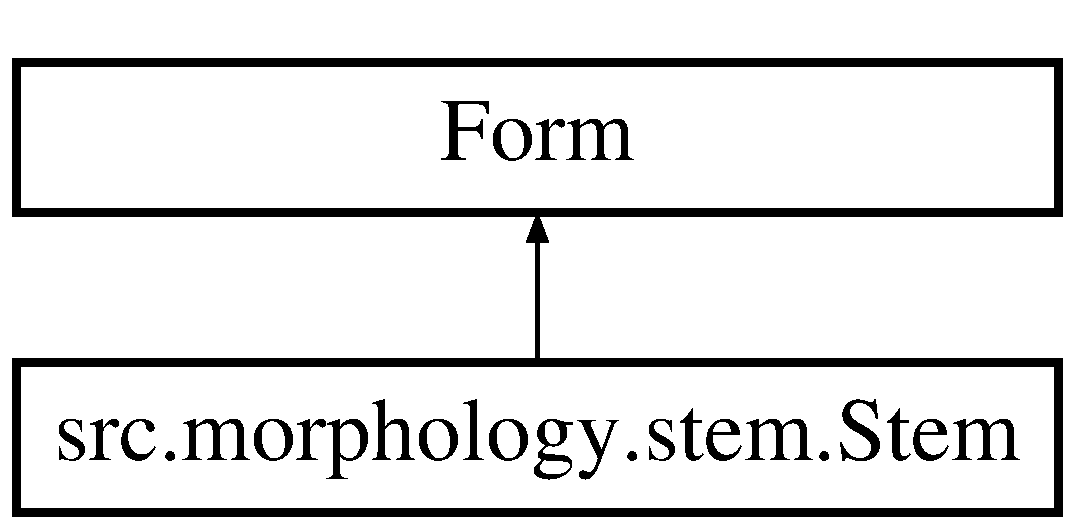
\includegraphics[height=2.000000cm]{classsrc_1_1morphology_1_1stem_1_1_stem}
\end{center}
\end{figure}
\subsection*{Public Member Functions}
\begin{DoxyCompactItemize}
\item 
def \hyperlink{classsrc_1_1morphology_1_1stem_1_1_stem_a8af7e8adc4f76994ac9417d0e7b8cd06}{\+\_\+\+\_\+init\+\_\+\+\_\+}
\end{DoxyCompactItemize}


\subsection{Detailed Description}


Definition at line 5 of file stem.\+py.



\subsection{Constructor \& Destructor Documentation}
\hypertarget{classsrc_1_1morphology_1_1stem_1_1_stem_a8af7e8adc4f76994ac9417d0e7b8cd06}{\index{src\+::morphology\+::stem\+::\+Stem@{src\+::morphology\+::stem\+::\+Stem}!\+\_\+\+\_\+init\+\_\+\+\_\+@{\+\_\+\+\_\+init\+\_\+\+\_\+}}
\index{\+\_\+\+\_\+init\+\_\+\+\_\+@{\+\_\+\+\_\+init\+\_\+\+\_\+}!src\+::morphology\+::stem\+::\+Stem@{src\+::morphology\+::stem\+::\+Stem}}
\subsubsection[{\+\_\+\+\_\+init\+\_\+\+\_\+}]{\setlength{\rightskip}{0pt plus 5cm}def src.\+morphology.\+stem.\+Stem.\+\_\+\+\_\+init\+\_\+\+\_\+ (
\begin{DoxyParamCaption}
\item[{}]{self}
\end{DoxyParamCaption}
)}}\label{classsrc_1_1morphology_1_1stem_1_1_stem_a8af7e8adc4f76994ac9417d0e7b8cd06}


Definition at line 6 of file stem.\+py.



The documentation for this class was generated from the following file\+:\begin{DoxyCompactItemize}
\item 
/\+Users/celine/\+Work/\+C\+N\+R\+S/workspace/\+Himal\+Co/dev/lib/lmf/src/morphology/\hyperlink{stem_8py}{stem.\+py}\end{DoxyCompactItemize}

\hypertarget{classsrc_1_1mrd_1_1subject__field_1_1_subject_field}{\section{src.\+mrd.\+subject\+\_\+field.\+Subject\+Field Class Reference}
\label{classsrc_1_1mrd_1_1subject__field_1_1_subject_field}\index{src.\+mrd.\+subject\+\_\+field.\+Subject\+Field@{src.\+mrd.\+subject\+\_\+field.\+Subject\+Field}}
}
\subsection*{Public Member Functions}
\begin{DoxyCompactItemize}
\item 
def \hyperlink{classsrc_1_1mrd_1_1subject__field_1_1_subject_field_a3eefbd187b50f3befa0169c72a287991}{\+\_\+\+\_\+init\+\_\+\+\_\+}
\end{DoxyCompactItemize}
\subsection*{Public Attributes}
\begin{DoxyCompactItemize}
\item 
\hyperlink{classsrc_1_1mrd_1_1subject__field_1_1_subject_field_ab7baf8a7df0ac57286e05d3f8442424e}{language}
\item 
\hyperlink{classsrc_1_1mrd_1_1subject__field_1_1_subject_field_a06a0125c3d3f9b33c5fad6a89994a123}{semantic\+Domain}
\end{DoxyCompactItemize}


\subsection{Detailed Description}


Definition at line 3 of file subject\+\_\+field.\+py.



\subsection{Constructor \& Destructor Documentation}
\hypertarget{classsrc_1_1mrd_1_1subject__field_1_1_subject_field_a3eefbd187b50f3befa0169c72a287991}{\index{src\+::mrd\+::subject\+\_\+field\+::\+Subject\+Field@{src\+::mrd\+::subject\+\_\+field\+::\+Subject\+Field}!\+\_\+\+\_\+init\+\_\+\+\_\+@{\+\_\+\+\_\+init\+\_\+\+\_\+}}
\index{\+\_\+\+\_\+init\+\_\+\+\_\+@{\+\_\+\+\_\+init\+\_\+\+\_\+}!src\+::mrd\+::subject\+\_\+field\+::\+Subject\+Field@{src\+::mrd\+::subject\+\_\+field\+::\+Subject\+Field}}
\subsubsection[{\+\_\+\+\_\+init\+\_\+\+\_\+}]{\setlength{\rightskip}{0pt plus 5cm}def src.\+mrd.\+subject\+\_\+field.\+Subject\+Field.\+\_\+\+\_\+init\+\_\+\+\_\+ (
\begin{DoxyParamCaption}
\item[{}]{self}
\end{DoxyParamCaption}
)}}\label{classsrc_1_1mrd_1_1subject__field_1_1_subject_field_a3eefbd187b50f3befa0169c72a287991}


Definition at line 4 of file subject\+\_\+field.\+py.



\subsection{Member Data Documentation}
\hypertarget{classsrc_1_1mrd_1_1subject__field_1_1_subject_field_ab7baf8a7df0ac57286e05d3f8442424e}{\index{src\+::mrd\+::subject\+\_\+field\+::\+Subject\+Field@{src\+::mrd\+::subject\+\_\+field\+::\+Subject\+Field}!language@{language}}
\index{language@{language}!src\+::mrd\+::subject\+\_\+field\+::\+Subject\+Field@{src\+::mrd\+::subject\+\_\+field\+::\+Subject\+Field}}
\subsubsection[{language}]{\setlength{\rightskip}{0pt plus 5cm}src.\+mrd.\+subject\+\_\+field.\+Subject\+Field.\+language}}\label{classsrc_1_1mrd_1_1subject__field_1_1_subject_field_ab7baf8a7df0ac57286e05d3f8442424e}


Definition at line 5 of file subject\+\_\+field.\+py.

\hypertarget{classsrc_1_1mrd_1_1subject__field_1_1_subject_field_a06a0125c3d3f9b33c5fad6a89994a123}{\index{src\+::mrd\+::subject\+\_\+field\+::\+Subject\+Field@{src\+::mrd\+::subject\+\_\+field\+::\+Subject\+Field}!semantic\+Domain@{semantic\+Domain}}
\index{semantic\+Domain@{semantic\+Domain}!src\+::mrd\+::subject\+\_\+field\+::\+Subject\+Field@{src\+::mrd\+::subject\+\_\+field\+::\+Subject\+Field}}
\subsubsection[{semantic\+Domain}]{\setlength{\rightskip}{0pt plus 5cm}src.\+mrd.\+subject\+\_\+field.\+Subject\+Field.\+semantic\+Domain}}\label{classsrc_1_1mrd_1_1subject__field_1_1_subject_field_a06a0125c3d3f9b33c5fad6a89994a123}


Definition at line 6 of file subject\+\_\+field.\+py.



The documentation for this class was generated from the following file\+:\begin{DoxyCompactItemize}
\item 
/\+Users/celine/\+Work/\+C\+N\+R\+S/workspace/\+Himal\+Co/dev/lib/lmf/src/mrd/\hyperlink{subject__field_8py}{subject\+\_\+field.\+py}\end{DoxyCompactItemize}

\hypertarget{classsrc_1_1core_1_1text__representation_1_1_text_representation}{\section{src.\+core.\+text\+\_\+representation.\+Text\+Representation Class Reference}
\label{classsrc_1_1core_1_1text__representation_1_1_text_representation}\index{src.\+core.\+text\+\_\+representation.\+Text\+Representation@{src.\+core.\+text\+\_\+representation.\+Text\+Representation}}
}
Inheritance diagram for src.\+core.\+text\+\_\+representation.\+Text\+Representation\+:\begin{figure}[H]
\begin{center}
\leavevmode
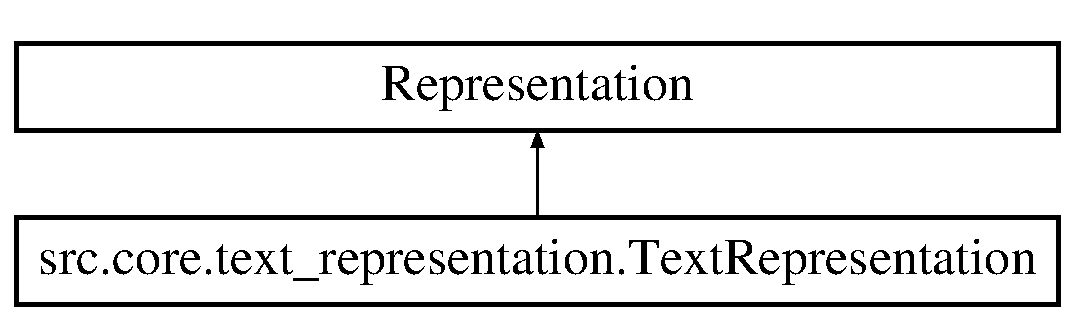
\includegraphics[height=2.000000cm]{classsrc_1_1core_1_1text__representation_1_1_text_representation}
\end{center}
\end{figure}
\subsection*{Public Member Functions}
\begin{DoxyCompactItemize}
\item 
def \hyperlink{classsrc_1_1core_1_1text__representation_1_1_text_representation_a4e022375d60b50b1b84aac1083650c4b}{\+\_\+\+\_\+init\+\_\+\+\_\+}
\end{DoxyCompactItemize}
\subsection*{Public Attributes}
\begin{DoxyCompactItemize}
\item 
\hyperlink{classsrc_1_1core_1_1text__representation_1_1_text_representation_aeb2f021498890dec4d8daff88cf704b8}{font}
\end{DoxyCompactItemize}


\subsection{Detailed Description}


Definition at line 5 of file text\+\_\+representation.\+py.



\subsection{Constructor \& Destructor Documentation}
\hypertarget{classsrc_1_1core_1_1text__representation_1_1_text_representation_a4e022375d60b50b1b84aac1083650c4b}{\index{src\+::core\+::text\+\_\+representation\+::\+Text\+Representation@{src\+::core\+::text\+\_\+representation\+::\+Text\+Representation}!\+\_\+\+\_\+init\+\_\+\+\_\+@{\+\_\+\+\_\+init\+\_\+\+\_\+}}
\index{\+\_\+\+\_\+init\+\_\+\+\_\+@{\+\_\+\+\_\+init\+\_\+\+\_\+}!src\+::core\+::text\+\_\+representation\+::\+Text\+Representation@{src\+::core\+::text\+\_\+representation\+::\+Text\+Representation}}
\subsubsection[{\+\_\+\+\_\+init\+\_\+\+\_\+}]{\setlength{\rightskip}{0pt plus 5cm}def src.\+core.\+text\+\_\+representation.\+Text\+Representation.\+\_\+\+\_\+init\+\_\+\+\_\+ (
\begin{DoxyParamCaption}
\item[{}]{self}
\end{DoxyParamCaption}
)}}\label{classsrc_1_1core_1_1text__representation_1_1_text_representation_a4e022375d60b50b1b84aac1083650c4b}


Definition at line 6 of file text\+\_\+representation.\+py.



\subsection{Member Data Documentation}
\hypertarget{classsrc_1_1core_1_1text__representation_1_1_text_representation_aeb2f021498890dec4d8daff88cf704b8}{\index{src\+::core\+::text\+\_\+representation\+::\+Text\+Representation@{src\+::core\+::text\+\_\+representation\+::\+Text\+Representation}!font@{font}}
\index{font@{font}!src\+::core\+::text\+\_\+representation\+::\+Text\+Representation@{src\+::core\+::text\+\_\+representation\+::\+Text\+Representation}}
\subsubsection[{font}]{\setlength{\rightskip}{0pt plus 5cm}src.\+core.\+text\+\_\+representation.\+Text\+Representation.\+font}}\label{classsrc_1_1core_1_1text__representation_1_1_text_representation_aeb2f021498890dec4d8daff88cf704b8}


Definition at line 7 of file text\+\_\+representation.\+py.



The documentation for this class was generated from the following file\+:\begin{DoxyCompactItemize}
\item 
/\+Users/celine/\+Work/\+C\+N\+R\+S/workspace/\+Himal\+Co/dev/lib/lmf/src/core/\hyperlink{text__representation_8py}{text\+\_\+representation.\+py}\end{DoxyCompactItemize}

\hypertarget{classsrc_1_1resources_1_1video_1_1_video}{\section{src.\+resources.\+video.\+Video Class Reference}
\label{classsrc_1_1resources_1_1video_1_1_video}\index{src.\+resources.\+video.\+Video@{src.\+resources.\+video.\+Video}}
}
Inheritance diagram for src.\+resources.\+video.\+Video\+:\begin{figure}[H]
\begin{center}
\leavevmode
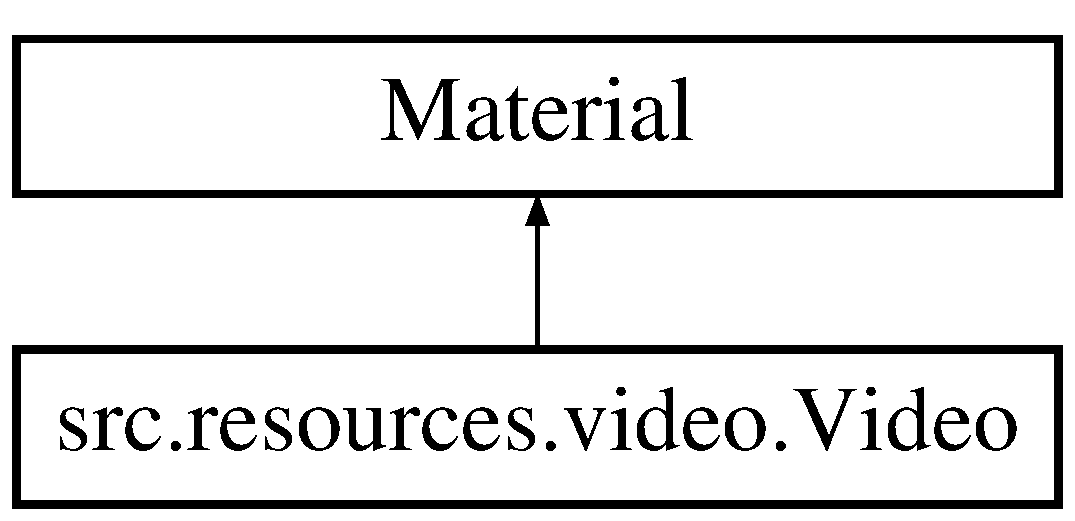
\includegraphics[height=2.000000cm]{classsrc_1_1resources_1_1video_1_1_video}
\end{center}
\end{figure}
\subsection*{Public Member Functions}
\begin{DoxyCompactItemize}
\item 
def \hyperlink{classsrc_1_1resources_1_1video_1_1_video_a715a09e9bc39544de57c1cf9a10da491}{\+\_\+\+\_\+init\+\_\+\+\_\+}
\end{DoxyCompactItemize}
\subsection*{Public Attributes}
\begin{DoxyCompactItemize}
\item 
\hyperlink{classsrc_1_1resources_1_1video_1_1_video_a0dc8832c83f1d52f217a6df00f755493}{description}
\end{DoxyCompactItemize}


\subsection{Detailed Description}


Definition at line 5 of file video.\+py.



\subsection{Constructor \& Destructor Documentation}
\hypertarget{classsrc_1_1resources_1_1video_1_1_video_a715a09e9bc39544de57c1cf9a10da491}{\index{src\+::resources\+::video\+::\+Video@{src\+::resources\+::video\+::\+Video}!\+\_\+\+\_\+init\+\_\+\+\_\+@{\+\_\+\+\_\+init\+\_\+\+\_\+}}
\index{\+\_\+\+\_\+init\+\_\+\+\_\+@{\+\_\+\+\_\+init\+\_\+\+\_\+}!src\+::resources\+::video\+::\+Video@{src\+::resources\+::video\+::\+Video}}
\subsubsection[{\+\_\+\+\_\+init\+\_\+\+\_\+}]{\setlength{\rightskip}{0pt plus 5cm}def src.\+resources.\+video.\+Video.\+\_\+\+\_\+init\+\_\+\+\_\+ (
\begin{DoxyParamCaption}
\item[{}]{self}
\end{DoxyParamCaption}
)}}\label{classsrc_1_1resources_1_1video_1_1_video_a715a09e9bc39544de57c1cf9a10da491}


Definition at line 6 of file video.\+py.



\subsection{Member Data Documentation}
\hypertarget{classsrc_1_1resources_1_1video_1_1_video_a0dc8832c83f1d52f217a6df00f755493}{\index{src\+::resources\+::video\+::\+Video@{src\+::resources\+::video\+::\+Video}!description@{description}}
\index{description@{description}!src\+::resources\+::video\+::\+Video@{src\+::resources\+::video\+::\+Video}}
\subsubsection[{description}]{\setlength{\rightskip}{0pt plus 5cm}src.\+resources.\+video.\+Video.\+description}}\label{classsrc_1_1resources_1_1video_1_1_video_a0dc8832c83f1d52f217a6df00f755493}


Definition at line 7 of file video.\+py.



The documentation for this class was generated from the following file\+:\begin{DoxyCompactItemize}
\item 
/\+Users/celine/\+Work/\+C\+N\+R\+S/workspace/\+Himal\+Co/dev/lib/lmf/src/resources/\hyperlink{video_8py}{video.\+py}\end{DoxyCompactItemize}

\hypertarget{classsrc_1_1morphology_1_1word__form_1_1_word_form}{\section{src.\+morphology.\+word\+\_\+form.\+Word\+Form Class Reference}
\label{classsrc_1_1morphology_1_1word__form_1_1_word_form}\index{src.\+morphology.\+word\+\_\+form.\+Word\+Form@{src.\+morphology.\+word\+\_\+form.\+Word\+Form}}
}
Inheritance diagram for src.\+morphology.\+word\+\_\+form.\+Word\+Form\+:\begin{figure}[H]
\begin{center}
\leavevmode
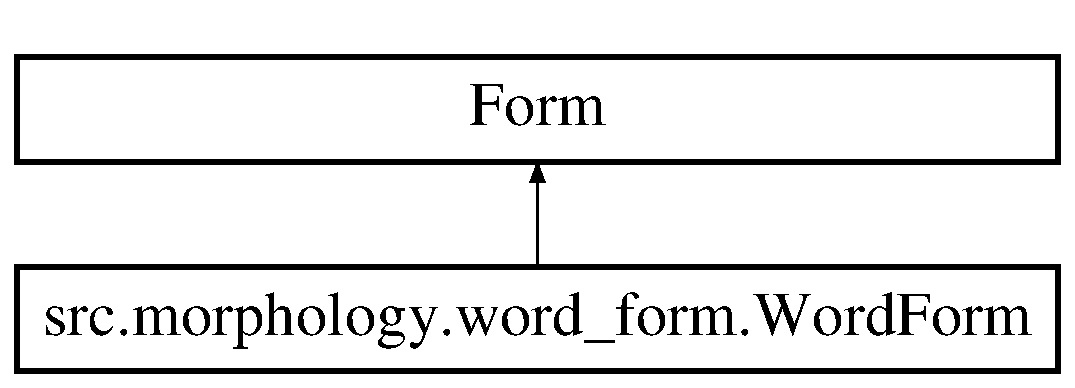
\includegraphics[height=2.000000cm]{classsrc_1_1morphology_1_1word__form_1_1_word_form}
\end{center}
\end{figure}
\subsection*{Public Member Functions}
\begin{DoxyCompactItemize}
\item 
def \hyperlink{classsrc_1_1morphology_1_1word__form_1_1_word_form_a739f72b577db8e5cf86463a0d82bbe05}{\+\_\+\+\_\+init\+\_\+\+\_\+}
\end{DoxyCompactItemize}
\subsection*{Public Attributes}
\begin{DoxyCompactItemize}
\item 
\hyperlink{classsrc_1_1morphology_1_1word__form_1_1_word_form_affc0a3ba96904019be2b92d55e832bcb}{grammatical\+Number}
\item 
\hyperlink{classsrc_1_1morphology_1_1word__form_1_1_word_form_a44467b3575140671b680bca5ee0b0483}{grammatical\+Gender}
\item 
\hyperlink{classsrc_1_1morphology_1_1word__form_1_1_word_form_a8c2487c9b360cc067bcb40ee7cf8d8c5}{person}
\item 
\hyperlink{classsrc_1_1morphology_1_1word__form_1_1_word_form_aa82c3234c1c9f209b7b8d6b2e3c3c246}{anymacy}
\item 
\hyperlink{classsrc_1_1morphology_1_1word__form_1_1_word_form_a04e4f04ce56e4a9628b8ceea29b4573c}{clusivity}
\item 
\hyperlink{classsrc_1_1morphology_1_1word__form_1_1_word_form_a1436b5d9574c2a0096b46fa607424576}{tense}
\item 
\hyperlink{classsrc_1_1morphology_1_1word__form_1_1_word_form_ab7de838ba2c0638094e58d2decd238af}{case}
\item 
\hyperlink{classsrc_1_1morphology_1_1word__form_1_1_word_form_adf2ee9bb3f0c2618cb4aaa6065300531}{degree}
\item 
\hyperlink{classsrc_1_1morphology_1_1word__form_1_1_word_form_ac6fbf70d32545170d2b203a58532706d}{voice}
\item 
\hyperlink{classsrc_1_1morphology_1_1word__form_1_1_word_form_a5af5bbdaf2247140e5379dbcf4994ec9}{verb\+Form\+Mood}
\end{DoxyCompactItemize}


\subsection{Detailed Description}


Definition at line 5 of file word\+\_\+form.\+py.



\subsection{Constructor \& Destructor Documentation}
\hypertarget{classsrc_1_1morphology_1_1word__form_1_1_word_form_a739f72b577db8e5cf86463a0d82bbe05}{\index{src\+::morphology\+::word\+\_\+form\+::\+Word\+Form@{src\+::morphology\+::word\+\_\+form\+::\+Word\+Form}!\+\_\+\+\_\+init\+\_\+\+\_\+@{\+\_\+\+\_\+init\+\_\+\+\_\+}}
\index{\+\_\+\+\_\+init\+\_\+\+\_\+@{\+\_\+\+\_\+init\+\_\+\+\_\+}!src\+::morphology\+::word\+\_\+form\+::\+Word\+Form@{src\+::morphology\+::word\+\_\+form\+::\+Word\+Form}}
\subsubsection[{\+\_\+\+\_\+init\+\_\+\+\_\+}]{\setlength{\rightskip}{0pt plus 5cm}def src.\+morphology.\+word\+\_\+form.\+Word\+Form.\+\_\+\+\_\+init\+\_\+\+\_\+ (
\begin{DoxyParamCaption}
\item[{}]{self}
\end{DoxyParamCaption}
)}}\label{classsrc_1_1morphology_1_1word__form_1_1_word_form_a739f72b577db8e5cf86463a0d82bbe05}


Definition at line 6 of file word\+\_\+form.\+py.



\subsection{Member Data Documentation}
\hypertarget{classsrc_1_1morphology_1_1word__form_1_1_word_form_aa82c3234c1c9f209b7b8d6b2e3c3c246}{\index{src\+::morphology\+::word\+\_\+form\+::\+Word\+Form@{src\+::morphology\+::word\+\_\+form\+::\+Word\+Form}!anymacy@{anymacy}}
\index{anymacy@{anymacy}!src\+::morphology\+::word\+\_\+form\+::\+Word\+Form@{src\+::morphology\+::word\+\_\+form\+::\+Word\+Form}}
\subsubsection[{anymacy}]{\setlength{\rightskip}{0pt plus 5cm}src.\+morphology.\+word\+\_\+form.\+Word\+Form.\+anymacy}}\label{classsrc_1_1morphology_1_1word__form_1_1_word_form_aa82c3234c1c9f209b7b8d6b2e3c3c246}


Definition at line 10 of file word\+\_\+form.\+py.

\hypertarget{classsrc_1_1morphology_1_1word__form_1_1_word_form_ab7de838ba2c0638094e58d2decd238af}{\index{src\+::morphology\+::word\+\_\+form\+::\+Word\+Form@{src\+::morphology\+::word\+\_\+form\+::\+Word\+Form}!case@{case}}
\index{case@{case}!src\+::morphology\+::word\+\_\+form\+::\+Word\+Form@{src\+::morphology\+::word\+\_\+form\+::\+Word\+Form}}
\subsubsection[{case}]{\setlength{\rightskip}{0pt plus 5cm}src.\+morphology.\+word\+\_\+form.\+Word\+Form.\+case}}\label{classsrc_1_1morphology_1_1word__form_1_1_word_form_ab7de838ba2c0638094e58d2decd238af}


Definition at line 13 of file word\+\_\+form.\+py.

\hypertarget{classsrc_1_1morphology_1_1word__form_1_1_word_form_a04e4f04ce56e4a9628b8ceea29b4573c}{\index{src\+::morphology\+::word\+\_\+form\+::\+Word\+Form@{src\+::morphology\+::word\+\_\+form\+::\+Word\+Form}!clusivity@{clusivity}}
\index{clusivity@{clusivity}!src\+::morphology\+::word\+\_\+form\+::\+Word\+Form@{src\+::morphology\+::word\+\_\+form\+::\+Word\+Form}}
\subsubsection[{clusivity}]{\setlength{\rightskip}{0pt plus 5cm}src.\+morphology.\+word\+\_\+form.\+Word\+Form.\+clusivity}}\label{classsrc_1_1morphology_1_1word__form_1_1_word_form_a04e4f04ce56e4a9628b8ceea29b4573c}


Definition at line 11 of file word\+\_\+form.\+py.

\hypertarget{classsrc_1_1morphology_1_1word__form_1_1_word_form_adf2ee9bb3f0c2618cb4aaa6065300531}{\index{src\+::morphology\+::word\+\_\+form\+::\+Word\+Form@{src\+::morphology\+::word\+\_\+form\+::\+Word\+Form}!degree@{degree}}
\index{degree@{degree}!src\+::morphology\+::word\+\_\+form\+::\+Word\+Form@{src\+::morphology\+::word\+\_\+form\+::\+Word\+Form}}
\subsubsection[{degree}]{\setlength{\rightskip}{0pt plus 5cm}src.\+morphology.\+word\+\_\+form.\+Word\+Form.\+degree}}\label{classsrc_1_1morphology_1_1word__form_1_1_word_form_adf2ee9bb3f0c2618cb4aaa6065300531}


Definition at line 14 of file word\+\_\+form.\+py.

\hypertarget{classsrc_1_1morphology_1_1word__form_1_1_word_form_a44467b3575140671b680bca5ee0b0483}{\index{src\+::morphology\+::word\+\_\+form\+::\+Word\+Form@{src\+::morphology\+::word\+\_\+form\+::\+Word\+Form}!grammatical\+Gender@{grammatical\+Gender}}
\index{grammatical\+Gender@{grammatical\+Gender}!src\+::morphology\+::word\+\_\+form\+::\+Word\+Form@{src\+::morphology\+::word\+\_\+form\+::\+Word\+Form}}
\subsubsection[{grammatical\+Gender}]{\setlength{\rightskip}{0pt plus 5cm}src.\+morphology.\+word\+\_\+form.\+Word\+Form.\+grammatical\+Gender}}\label{classsrc_1_1morphology_1_1word__form_1_1_word_form_a44467b3575140671b680bca5ee0b0483}


Definition at line 8 of file word\+\_\+form.\+py.

\hypertarget{classsrc_1_1morphology_1_1word__form_1_1_word_form_affc0a3ba96904019be2b92d55e832bcb}{\index{src\+::morphology\+::word\+\_\+form\+::\+Word\+Form@{src\+::morphology\+::word\+\_\+form\+::\+Word\+Form}!grammatical\+Number@{grammatical\+Number}}
\index{grammatical\+Number@{grammatical\+Number}!src\+::morphology\+::word\+\_\+form\+::\+Word\+Form@{src\+::morphology\+::word\+\_\+form\+::\+Word\+Form}}
\subsubsection[{grammatical\+Number}]{\setlength{\rightskip}{0pt plus 5cm}src.\+morphology.\+word\+\_\+form.\+Word\+Form.\+grammatical\+Number}}\label{classsrc_1_1morphology_1_1word__form_1_1_word_form_affc0a3ba96904019be2b92d55e832bcb}


Definition at line 7 of file word\+\_\+form.\+py.

\hypertarget{classsrc_1_1morphology_1_1word__form_1_1_word_form_a8c2487c9b360cc067bcb40ee7cf8d8c5}{\index{src\+::morphology\+::word\+\_\+form\+::\+Word\+Form@{src\+::morphology\+::word\+\_\+form\+::\+Word\+Form}!person@{person}}
\index{person@{person}!src\+::morphology\+::word\+\_\+form\+::\+Word\+Form@{src\+::morphology\+::word\+\_\+form\+::\+Word\+Form}}
\subsubsection[{person}]{\setlength{\rightskip}{0pt plus 5cm}src.\+morphology.\+word\+\_\+form.\+Word\+Form.\+person}}\label{classsrc_1_1morphology_1_1word__form_1_1_word_form_a8c2487c9b360cc067bcb40ee7cf8d8c5}


Definition at line 9 of file word\+\_\+form.\+py.

\hypertarget{classsrc_1_1morphology_1_1word__form_1_1_word_form_a1436b5d9574c2a0096b46fa607424576}{\index{src\+::morphology\+::word\+\_\+form\+::\+Word\+Form@{src\+::morphology\+::word\+\_\+form\+::\+Word\+Form}!tense@{tense}}
\index{tense@{tense}!src\+::morphology\+::word\+\_\+form\+::\+Word\+Form@{src\+::morphology\+::word\+\_\+form\+::\+Word\+Form}}
\subsubsection[{tense}]{\setlength{\rightskip}{0pt plus 5cm}src.\+morphology.\+word\+\_\+form.\+Word\+Form.\+tense}}\label{classsrc_1_1morphology_1_1word__form_1_1_word_form_a1436b5d9574c2a0096b46fa607424576}


Definition at line 12 of file word\+\_\+form.\+py.

\hypertarget{classsrc_1_1morphology_1_1word__form_1_1_word_form_a5af5bbdaf2247140e5379dbcf4994ec9}{\index{src\+::morphology\+::word\+\_\+form\+::\+Word\+Form@{src\+::morphology\+::word\+\_\+form\+::\+Word\+Form}!verb\+Form\+Mood@{verb\+Form\+Mood}}
\index{verb\+Form\+Mood@{verb\+Form\+Mood}!src\+::morphology\+::word\+\_\+form\+::\+Word\+Form@{src\+::morphology\+::word\+\_\+form\+::\+Word\+Form}}
\subsubsection[{verb\+Form\+Mood}]{\setlength{\rightskip}{0pt plus 5cm}src.\+morphology.\+word\+\_\+form.\+Word\+Form.\+verb\+Form\+Mood}}\label{classsrc_1_1morphology_1_1word__form_1_1_word_form_a5af5bbdaf2247140e5379dbcf4994ec9}


Definition at line 16 of file word\+\_\+form.\+py.

\hypertarget{classsrc_1_1morphology_1_1word__form_1_1_word_form_ac6fbf70d32545170d2b203a58532706d}{\index{src\+::morphology\+::word\+\_\+form\+::\+Word\+Form@{src\+::morphology\+::word\+\_\+form\+::\+Word\+Form}!voice@{voice}}
\index{voice@{voice}!src\+::morphology\+::word\+\_\+form\+::\+Word\+Form@{src\+::morphology\+::word\+\_\+form\+::\+Word\+Form}}
\subsubsection[{voice}]{\setlength{\rightskip}{0pt plus 5cm}src.\+morphology.\+word\+\_\+form.\+Word\+Form.\+voice}}\label{classsrc_1_1morphology_1_1word__form_1_1_word_form_ac6fbf70d32545170d2b203a58532706d}


Definition at line 15 of file word\+\_\+form.\+py.



The documentation for this class was generated from the following file\+:\begin{DoxyCompactItemize}
\item 
/\+Users/celine/\+Work/\+C\+N\+R\+S/workspace/\+Himal\+Co/dev/lib/lmf/src/morphology/\hyperlink{word__form_8py}{word\+\_\+form.\+py}\end{DoxyCompactItemize}

\chapter{File Documentation}
\hypertarget{____init_____8py}{\section{/\+Users/celine/\+Work/\+C\+N\+R\+S/workspace/\+Himal\+Co/dev/lib/lmf/src/\+\_\+\+\_\+init\+\_\+\+\_\+.py File Reference}
\label{____init_____8py}\index{/\+Users/celine/\+Work/\+C\+N\+R\+S/workspace/\+Himal\+Co/dev/lib/lmf/src/\+\_\+\+\_\+init\+\_\+\+\_\+.\+py@{/\+Users/celine/\+Work/\+C\+N\+R\+S/workspace/\+Himal\+Co/dev/lib/lmf/src/\+\_\+\+\_\+init\+\_\+\+\_\+.\+py}}
}
\subsection*{Namespaces}
\begin{DoxyCompactItemize}
\item 
 \hyperlink{namespacelmf_1_1src}{lmf.\+src}
\end{DoxyCompactItemize}

\hypertarget{common_2____init_____8py}{\section{/\+Users/celine/\+Work/\+C\+N\+R\+S/workspace/\+Himal\+Co/dev/lib/lmf/src/common/\+\_\+\+\_\+init\+\_\+\+\_\+.py File Reference}
\label{common_2____init_____8py}\index{/\+Users/celine/\+Work/\+C\+N\+R\+S/workspace/\+Himal\+Co/dev/lib/lmf/src/common/\+\_\+\+\_\+init\+\_\+\+\_\+.\+py@{/\+Users/celine/\+Work/\+C\+N\+R\+S/workspace/\+Himal\+Co/dev/lib/lmf/src/common/\+\_\+\+\_\+init\+\_\+\+\_\+.\+py}}
}
\subsection*{Namespaces}
\begin{DoxyCompactItemize}
\item 
 \hyperlink{namespacelmf_1_1src_1_1common}{lmf.\+src.\+common}
\end{DoxyCompactItemize}

\hypertarget{config_2____init_____8py}{\section{/\+Users/celine/\+Work/\+C\+N\+R\+S/workspace/\+Himal\+Co/dev/lib/lmf/src/config/\+\_\+\+\_\+init\+\_\+\+\_\+.py File Reference}
\label{config_2____init_____8py}\index{/\+Users/celine/\+Work/\+C\+N\+R\+S/workspace/\+Himal\+Co/dev/lib/lmf/src/config/\+\_\+\+\_\+init\+\_\+\+\_\+.\+py@{/\+Users/celine/\+Work/\+C\+N\+R\+S/workspace/\+Himal\+Co/dev/lib/lmf/src/config/\+\_\+\+\_\+init\+\_\+\+\_\+.\+py}}
}
\subsection*{Namespaces}
\begin{DoxyCompactItemize}
\item 
 \hyperlink{namespacesrc_1_1config}{src.\+config}
\end{DoxyCompactItemize}

\hypertarget{core_2____init_____8py}{\section{/\+Users/celine/\+Work/\+C\+N\+R\+S/workspace/\+Himal\+Co/dev/lib/lmf/src/core/\+\_\+\+\_\+init\+\_\+\+\_\+.py File Reference}
\label{core_2____init_____8py}\index{/\+Users/celine/\+Work/\+C\+N\+R\+S/workspace/\+Himal\+Co/dev/lib/lmf/src/core/\+\_\+\+\_\+init\+\_\+\+\_\+.\+py@{/\+Users/celine/\+Work/\+C\+N\+R\+S/workspace/\+Himal\+Co/dev/lib/lmf/src/core/\+\_\+\+\_\+init\+\_\+\+\_\+.\+py}}
}
\subsection*{Namespaces}
\begin{DoxyCompactItemize}
\item 
 \hyperlink{namespacelmf_1_1src_1_1core}{lmf.\+src.\+core}
\end{DoxyCompactItemize}

\hypertarget{input_2____init_____8py}{\section{/\+Users/celine/\+Work/\+C\+N\+R\+S/workspace/\+Himal\+Co/dev/lib/lmf/src/input/\+\_\+\+\_\+init\+\_\+\+\_\+.py File Reference}
\label{input_2____init_____8py}\index{/\+Users/celine/\+Work/\+C\+N\+R\+S/workspace/\+Himal\+Co/dev/lib/lmf/src/input/\+\_\+\+\_\+init\+\_\+\+\_\+.\+py@{/\+Users/celine/\+Work/\+C\+N\+R\+S/workspace/\+Himal\+Co/dev/lib/lmf/src/input/\+\_\+\+\_\+init\+\_\+\+\_\+.\+py}}
}
\subsection*{Namespaces}
\begin{DoxyCompactItemize}
\item 
 \hyperlink{namespacesrc_1_1input}{src.\+input}
\end{DoxyCompactItemize}

\hypertarget{morphology_2____init_____8py}{\section{/\+Users/celine/\+Work/\+C\+N\+R\+S/workspace/\+Himal\+Co/dev/lib/lmf/src/morphology/\+\_\+\+\_\+init\+\_\+\+\_\+.py File Reference}
\label{morphology_2____init_____8py}\index{/\+Users/celine/\+Work/\+C\+N\+R\+S/workspace/\+Himal\+Co/dev/lib/lmf/src/morphology/\+\_\+\+\_\+init\+\_\+\+\_\+.\+py@{/\+Users/celine/\+Work/\+C\+N\+R\+S/workspace/\+Himal\+Co/dev/lib/lmf/src/morphology/\+\_\+\+\_\+init\+\_\+\+\_\+.\+py}}
}
\subsection*{Namespaces}
\begin{DoxyCompactItemize}
\item 
 \hyperlink{namespacesrc_1_1morphology}{src.\+morphology}
\end{DoxyCompactItemize}

\hypertarget{morphosyntax_2____init_____8py}{\section{/\+Users/celine/\+Work/\+C\+N\+R\+S/workspace/\+Himal\+Co/dev/lib/lmf/src/morphosyntax/\+\_\+\+\_\+init\+\_\+\+\_\+.py File Reference}
\label{morphosyntax_2____init_____8py}\index{/\+Users/celine/\+Work/\+C\+N\+R\+S/workspace/\+Himal\+Co/dev/lib/lmf/src/morphosyntax/\+\_\+\+\_\+init\+\_\+\+\_\+.\+py@{/\+Users/celine/\+Work/\+C\+N\+R\+S/workspace/\+Himal\+Co/dev/lib/lmf/src/morphosyntax/\+\_\+\+\_\+init\+\_\+\+\_\+.\+py}}
}
\subsection*{Namespaces}
\begin{DoxyCompactItemize}
\item 
 \hyperlink{namespacesrc_1_1morphosyntax}{src.\+morphosyntax}
\end{DoxyCompactItemize}

\hypertarget{mrd_2____init_____8py}{\section{/\+Users/celine/\+Work/\+C\+N\+R\+S/workspace/\+Himal\+Co/dev/lib/lmf/src/mrd/\+\_\+\+\_\+init\+\_\+\+\_\+.py File Reference}
\label{mrd_2____init_____8py}\index{/\+Users/celine/\+Work/\+C\+N\+R\+S/workspace/\+Himal\+Co/dev/lib/lmf/src/mrd/\+\_\+\+\_\+init\+\_\+\+\_\+.\+py@{/\+Users/celine/\+Work/\+C\+N\+R\+S/workspace/\+Himal\+Co/dev/lib/lmf/src/mrd/\+\_\+\+\_\+init\+\_\+\+\_\+.\+py}}
}
\subsection*{Namespaces}
\begin{DoxyCompactItemize}
\item 
 \hyperlink{namespacelmf_1_1src_1_1mrd}{lmf.\+src.\+mrd}
\end{DoxyCompactItemize}

\hypertarget{output_2____init_____8py}{\section{/\+Users/celine/\+Work/\+C\+N\+R\+S/workspace/\+Himal\+Co/dev/lib/lmf/src/output/\+\_\+\+\_\+init\+\_\+\+\_\+.py File Reference}
\label{output_2____init_____8py}\index{/\+Users/celine/\+Work/\+C\+N\+R\+S/workspace/\+Himal\+Co/dev/lib/lmf/src/output/\+\_\+\+\_\+init\+\_\+\+\_\+.\+py@{/\+Users/celine/\+Work/\+C\+N\+R\+S/workspace/\+Himal\+Co/dev/lib/lmf/src/output/\+\_\+\+\_\+init\+\_\+\+\_\+.\+py}}
}
\subsection*{Namespaces}
\begin{DoxyCompactItemize}
\item 
 \hyperlink{namespacesrc_1_1output}{src.\+output}
\end{DoxyCompactItemize}

\hypertarget{resources_2____init_____8py}{\section{/\+Users/celine/\+Work/\+C\+N\+R\+S/workspace/\+Himal\+Co/dev/lib/lmf/src/resources/\+\_\+\+\_\+init\+\_\+\+\_\+.py File Reference}
\label{resources_2____init_____8py}\index{/\+Users/celine/\+Work/\+C\+N\+R\+S/workspace/\+Himal\+Co/dev/lib/lmf/src/resources/\+\_\+\+\_\+init\+\_\+\+\_\+.\+py@{/\+Users/celine/\+Work/\+C\+N\+R\+S/workspace/\+Himal\+Co/dev/lib/lmf/src/resources/\+\_\+\+\_\+init\+\_\+\+\_\+.\+py}}
}
\subsection*{Namespaces}
\begin{DoxyCompactItemize}
\item 
 \hyperlink{namespacesrc_1_1resources}{src.\+resources}
\end{DoxyCompactItemize}

\hypertarget{utils_2____init_____8py}{\section{/\+Users/celine/\+Work/\+C\+N\+R\+S/workspace/\+Himal\+Co/dev/lib/lmf/src/utils/\+\_\+\+\_\+init\+\_\+\+\_\+.py File Reference}
\label{utils_2____init_____8py}\index{/\+Users/celine/\+Work/\+C\+N\+R\+S/workspace/\+Himal\+Co/dev/lib/lmf/src/utils/\+\_\+\+\_\+init\+\_\+\+\_\+.\+py@{/\+Users/celine/\+Work/\+C\+N\+R\+S/workspace/\+Himal\+Co/dev/lib/lmf/src/utils/\+\_\+\+\_\+init\+\_\+\+\_\+.\+py}}
}
\subsection*{Namespaces}
\begin{DoxyCompactItemize}
\item 
 \hyperlink{namespacelmf_1_1src_1_1utils}{lmf.\+src.\+utils}
\end{DoxyCompactItemize}

\hypertarget{config_2mdf_8py}{\section{/\+Users/celine/\+Work/\+C\+N\+R\+S/workspace/\+Himal\+Co/dev/lib/lmf/src/config/mdf.py File Reference}
\label{config_2mdf_8py}\index{/\+Users/celine/\+Work/\+C\+N\+R\+S/workspace/\+Himal\+Co/dev/lib/lmf/src/config/mdf.\+py@{/\+Users/celine/\+Work/\+C\+N\+R\+S/workspace/\+Himal\+Co/dev/lib/lmf/src/config/mdf.\+py}}
}
\subsection*{Namespaces}
\begin{DoxyCompactItemize}
\item 
 \hyperlink{namespacelmf_1_1src_1_1config_1_1mdf}{lmf.\+src.\+config.\+mdf}
\end{DoxyCompactItemize}
\subsection*{Functions}
\begin{DoxyCompactItemize}
\item 
def \hyperlink{namespacelmf_1_1src_1_1config_1_1mdf_ab9d98a9297210440ed93a3ca490ee7b4}{lmf.\+src.\+config.\+mdf.\+set\+\_\+bw}
\begin{DoxyCompactList}\small\item\em Functions to process some M\+D\+F fields (input) \end{DoxyCompactList}\item 
def \hyperlink{namespacelmf_1_1src_1_1config_1_1mdf_a5af3cc74d2bb8b03d7657c0e7fb3598b}{lmf.\+src.\+config.\+mdf.\+get\+\_\+bw}
\begin{DoxyCompactList}\small\item\em Functions to process some M\+D\+F fields (output) \end{DoxyCompactList}\end{DoxyCompactItemize}
\subsection*{Variables}
\begin{DoxyCompactItemize}
\item 
tuple \hyperlink{namespacelmf_1_1src_1_1config_1_1mdf_a888cd9df8b9511d408e646dc404b5232}{lmf.\+src.\+config.\+mdf.\+mdf\+\_\+lmf}
\begin{DoxyCompactList}\small\item\em Mapping between M\+D\+F markers and L\+M\+F representation (input) \end{DoxyCompactList}\item 
list \hyperlink{namespacelmf_1_1src_1_1config_1_1mdf_afe5efb72442beb65b5083335b744845c}{lmf.\+src.\+config.\+mdf.\+mdf\+\_\+order}
\begin{DoxyCompactList}\small\item\em Order in which M\+D\+F markers must be written (output) This is the standard order defined in Appendix B of \char`\"{}\+Making Dictionaries. A guide to lexicography and the Multi-\/\+Dictionary Formatter\char`\"{}, Software version 1.\+0, David F. \end{DoxyCompactList}\item 
tuple \hyperlink{namespacelmf_1_1src_1_1config_1_1mdf_a78d8f1444783c1b86cbbd91f49a0cd4f}{lmf.\+src.\+config.\+mdf.\+lmf\+\_\+mdf}
\begin{DoxyCompactList}\small\item\em Mapping between L\+M\+F representation and M\+D\+F markers (output) \end{DoxyCompactList}\item 
tuple \hyperlink{namespacelmf_1_1src_1_1config_1_1mdf_a59bb4fce205d8159bc72c946e3855c4a}{lmf.\+src.\+config.\+mdf.\+ps\+\_\+range}
\begin{DoxyCompactList}\small\item\em Possible values allowed for 'ps' M\+D\+F marker. \end{DoxyCompactList}\item 
tuple \hyperlink{namespacelmf_1_1src_1_1config_1_1mdf_a1e76a452fc77f05851e4369134f5980b}{lmf.\+src.\+config.\+mdf.\+ps\+\_\+part\+Of\+Speech}
\begin{DoxyCompactList}\small\item\em Mapping between 'ps' M\+D\+F marker value and L\+M\+F part of speech Lexical\+Entry attribute value (input) Source\+: \href{http://www.isocat.org/rest/dcs/119}{\tt http\+://www.\+isocat.\+org/rest/dcs/119}. \end{DoxyCompactList}\item 
tuple \hyperlink{namespacelmf_1_1src_1_1config_1_1mdf_a20455cbc7aa64cc6eb4ad1749a381738}{lmf.\+src.\+config.\+mdf.\+mdf\+\_\+semantic\+Relation}
\begin{DoxyCompactList}\small\item\em Mapping between M\+D\+F markers and L\+M\+F semantic relation Related\+Form attribute value (input) \end{DoxyCompactList}\item 
tuple \hyperlink{namespacelmf_1_1src_1_1config_1_1mdf_ab58fb9b58bc32ac36efe9b26e4ea3ca2}{lmf.\+src.\+config.\+mdf.\+pd\+\_\+person}
\begin{DoxyCompactList}\small\item\em Mapping between 'pd' M\+D\+F markers and L\+M\+F person Word\+Form attribute value (input) \end{DoxyCompactList}\item 
tuple \hyperlink{namespacelmf_1_1src_1_1config_1_1mdf_a011f241f41e3620deefe53cbb42286b9}{lmf.\+src.\+config.\+mdf.\+pd\+\_\+anymacy}
\begin{DoxyCompactList}\small\item\em Mapping between 'pd' M\+D\+F markers and L\+M\+F anymacy Word\+Form attribute value (input) \end{DoxyCompactList}\item 
tuple \hyperlink{namespacelmf_1_1src_1_1config_1_1mdf_a64be26974728c369cd72ef80bd297154}{lmf.\+src.\+config.\+mdf.\+pd\+\_\+grammatical\+Number}
\begin{DoxyCompactList}\small\item\em Mapping between 'pd' M\+D\+F markers and L\+M\+F grammatical number Word\+Form attribute value (input) \end{DoxyCompactList}\item 
tuple \hyperlink{namespacelmf_1_1src_1_1config_1_1mdf_ac57ebe92cdf841d8d1bfe1e1b94b96bb}{lmf.\+src.\+config.\+mdf.\+pd\+\_\+clusivity}
\begin{DoxyCompactList}\small\item\em Mapping between 'pd' M\+D\+F markers and L\+M\+F clusivity Word\+Form attribute value (input) \end{DoxyCompactList}\item 
tuple \hyperlink{namespacelmf_1_1src_1_1config_1_1mdf_a8e61adc475ca415a33c85ef16c96d03d}{lmf.\+src.\+config.\+mdf.\+pdl\+\_\+paradigm\+Label}
\begin{DoxyCompactList}\small\item\em Mapping between 'pdl' M\+D\+F marker value and L\+M\+F paradigm label Paradigm attribute value (input) \end{DoxyCompactList}\item 
tuple \hyperlink{namespacelmf_1_1src_1_1config_1_1mdf_a69afee1e13ba980f4da1e6d7fb0c488a}{lmf.\+src.\+config.\+mdf.\+sd\+\_\+range}
\begin{DoxyCompactList}\small\item\em Possible values allowed for 'sd' M\+D\+F marker. \end{DoxyCompactList}\item 
tuple \hyperlink{namespacelmf_1_1src_1_1config_1_1mdf_a61a24538d210d4eca3f57f183733fa5a}{lmf.\+src.\+config.\+mdf.\+lf\+\_\+range}
\begin{DoxyCompactList}\small\item\em Possible values allowed for 'lf' M\+D\+F marker. \end{DoxyCompactList}\end{DoxyCompactItemize}

\hypertarget{input_2mdf_8py}{\section{/\+Users/celine/\+Work/\+C\+N\+R\+S/workspace/\+Himal\+Co/dev/lib/lmf/src/input/mdf.py File Reference}
\label{input_2mdf_8py}\index{/\+Users/celine/\+Work/\+C\+N\+R\+S/workspace/\+Himal\+Co/dev/lib/lmf/src/input/mdf.\+py@{/\+Users/celine/\+Work/\+C\+N\+R\+S/workspace/\+Himal\+Co/dev/lib/lmf/src/input/mdf.\+py}}
}
\subsection*{Namespaces}
\begin{DoxyCompactItemize}
\item 
 \hyperlink{namespacelmf_1_1src_1_1input_1_1mdf}{lmf.\+src.\+input.\+mdf}
\end{DoxyCompactItemize}
\subsection*{Functions}
\begin{DoxyCompactItemize}
\item 
def \hyperlink{namespacelmf_1_1src_1_1input_1_1mdf_adf21a8b8bd5a33be054269ced938ba52}{lmf.\+src.\+input.\+mdf.\+mdf\+\_\+read}
\begin{DoxyCompactList}\small\item\em Read an M\+D\+F file. \end{DoxyCompactList}\end{DoxyCompactItemize}

\hypertarget{output_2mdf_8py}{\section{/\+Users/celine/\+Work/\+C\+N\+R\+S/workspace/\+Himal\+Co/dev/lib/lmf/src/output/mdf.py File Reference}
\label{output_2mdf_8py}\index{/\+Users/celine/\+Work/\+C\+N\+R\+S/workspace/\+Himal\+Co/dev/lib/lmf/src/output/mdf.\+py@{/\+Users/celine/\+Work/\+C\+N\+R\+S/workspace/\+Himal\+Co/dev/lib/lmf/src/output/mdf.\+py}}
}
\subsection*{Namespaces}
\begin{DoxyCompactItemize}
\item 
 \hyperlink{namespacesrc_1_1output_1_1mdf}{src.\+output.\+mdf}
\end{DoxyCompactItemize}
\subsection*{Functions}
\begin{DoxyCompactItemize}
\item 
def \hyperlink{namespacesrc_1_1output_1_1mdf_a71397767dc07eda4ff1586de29e7c25d}{src.\+output.\+mdf.\+mdf\+\_\+write}
\begin{DoxyCompactList}\small\item\em Write an M\+D\+F file. \end{DoxyCompactList}\end{DoxyCompactItemize}

\hypertarget{config_2tex_8py}{\section{/\+Users/celine/\+Work/\+C\+N\+R\+S/workspace/\+Himal\+Co/dev/lib/lmf/src/config/tex.py File Reference}
\label{config_2tex_8py}\index{/\+Users/celine/\+Work/\+C\+N\+R\+S/workspace/\+Himal\+Co/dev/lib/lmf/src/config/tex.\+py@{/\+Users/celine/\+Work/\+C\+N\+R\+S/workspace/\+Himal\+Co/dev/lib/lmf/src/config/tex.\+py}}
}
\subsection*{Namespaces}
\begin{DoxyCompactItemize}
\item 
 \hyperlink{namespacelmf_1_1src_1_1config_1_1tex}{lmf.\+src.\+config.\+tex}
\end{DoxyCompactItemize}
\subsection*{Functions}
\begin{DoxyCompactItemize}
\item 
def \hyperlink{namespacelmf_1_1src_1_1config_1_1tex_ac85ca206e865c9cc1d77b77c72a429d2}{lmf.\+src.\+config.\+tex.\+lmf\+\_\+to\+\_\+tex}
\begin{DoxyCompactList}\small\item\em Function giving order in which information must be written in La\+Te\+X and mapping between L\+M\+F representation and La\+Te\+X (output) \end{DoxyCompactList}\end{DoxyCompactItemize}
\subsection*{Variables}
\begin{DoxyCompactItemize}
\item 
tuple \hyperlink{namespacelmf_1_1src_1_1config_1_1tex_a94016d28cbde962dd9dee1465bf19548}{lmf.\+src.\+config.\+tex.\+part\+Of\+Speech\+\_\+tex}
\begin{DoxyCompactList}\small\item\em Mapping between L\+M\+F part of speech Lexical\+Entry attribute value and La\+Te\+X layout (output) \end{DoxyCompactList}\item 
tuple \hyperlink{namespacelmf_1_1src_1_1config_1_1tex_a2a4c92ffc93b18380a5eb8971c518776}{lmf.\+src.\+config.\+tex.\+paradigm\+Label\+\_\+tex}
\begin{DoxyCompactList}\small\item\em Mapping between L\+M\+F paradigm\+Label Paradigm attribute value and La\+Te\+X layout (output) \end{DoxyCompactList}\end{DoxyCompactItemize}

\hypertarget{output_2tex_8py}{\section{/\+Users/celine/\+Work/\+C\+N\+R\+S/workspace/\+Himal\+Co/dev/lib/lmf/src/output/tex.py File Reference}
\label{output_2tex_8py}\index{/\+Users/celine/\+Work/\+C\+N\+R\+S/workspace/\+Himal\+Co/dev/lib/lmf/src/output/tex.\+py@{/\+Users/celine/\+Work/\+C\+N\+R\+S/workspace/\+Himal\+Co/dev/lib/lmf/src/output/tex.\+py}}
}
\subsection*{Namespaces}
\begin{DoxyCompactItemize}
\item 
 \hyperlink{namespacelmf_1_1src_1_1output_1_1tex}{lmf.\+src.\+output.\+tex}
\end{DoxyCompactItemize}
\subsection*{Functions}
\begin{DoxyCompactItemize}
\item 
def \hyperlink{namespacelmf_1_1src_1_1output_1_1tex_ac02be073e031d36d66f61dc7d6fb94df}{lmf.\+src.\+output.\+tex.\+compute\+\_\+header}
\begin{DoxyCompactList}\small\item\em Create La\+Te\+X header. \end{DoxyCompactList}\item 
def \hyperlink{namespacelmf_1_1src_1_1output_1_1tex_a2f69a7ff35d3a419eaa9f4bb40aefa06}{lmf.\+src.\+output.\+tex.\+tex\+\_\+write}
\begin{DoxyCompactList}\small\item\em Write a La\+Te\+X file. \end{DoxyCompactList}\end{DoxyCompactItemize}

\hypertarget{definition_8py}{\section{/\+Users/celine/\+Work/\+C\+N\+R\+S/workspace/\+Himal\+Co/dev/lib/lmf/src/core/definition.py File Reference}
\label{definition_8py}\index{/\+Users/celine/\+Work/\+C\+N\+R\+S/workspace/\+Himal\+Co/dev/lib/lmf/src/core/definition.\+py@{/\+Users/celine/\+Work/\+C\+N\+R\+S/workspace/\+Himal\+Co/dev/lib/lmf/src/core/definition.\+py}}
}
\subsection*{Classes}
\begin{DoxyCompactItemize}
\item 
class \hyperlink{classsrc_1_1core_1_1definition_1_1_definition}{src.\+core.\+definition.\+Definition}
\end{DoxyCompactItemize}
\subsection*{Namespaces}
\begin{DoxyCompactItemize}
\item 
 \hyperlink{namespacesrc_1_1core_1_1definition}{src.\+core.\+definition}
\end{DoxyCompactItemize}

\hypertarget{form_8py}{\section{/\+Users/celine/\+Work/\+C\+N\+R\+S/workspace/\+Himal\+Co/dev/lib/lmf/src/core/form.py File Reference}
\label{form_8py}\index{/\+Users/celine/\+Work/\+C\+N\+R\+S/workspace/\+Himal\+Co/dev/lib/lmf/src/core/form.\+py@{/\+Users/celine/\+Work/\+C\+N\+R\+S/workspace/\+Himal\+Co/dev/lib/lmf/src/core/form.\+py}}
}
\subsection*{Classes}
\begin{DoxyCompactItemize}
\item 
class \hyperlink{classsrc_1_1core_1_1form_1_1_form}{src.\+core.\+form.\+Form}
\end{DoxyCompactItemize}
\subsection*{Namespaces}
\begin{DoxyCompactItemize}
\item 
 \hyperlink{namespacesrc_1_1core_1_1form}{src.\+core.\+form}
\end{DoxyCompactItemize}

\hypertarget{form__representation_8py}{\section{/\+Users/celine/\+Work/\+C\+N\+R\+S/workspace/\+Himal\+Co/dev/lib/lmf/src/core/form\+\_\+representation.py File Reference}
\label{form__representation_8py}\index{/\+Users/celine/\+Work/\+C\+N\+R\+S/workspace/\+Himal\+Co/dev/lib/lmf/src/core/form\+\_\+representation.\+py@{/\+Users/celine/\+Work/\+C\+N\+R\+S/workspace/\+Himal\+Co/dev/lib/lmf/src/core/form\+\_\+representation.\+py}}
}
\subsection*{Classes}
\begin{DoxyCompactItemize}
\item 
class \hyperlink{classlmf_1_1src_1_1core_1_1form__representation_1_1_form_representation}{lmf.\+src.\+core.\+form\+\_\+representation.\+Form\+Representation}
\begin{DoxyCompactList}\small\item\em \char`\"{}\+Form Representation is a class representing one variant orthography of a Form.\char`\"{} (L\+M\+F) \end{DoxyCompactList}\end{DoxyCompactItemize}
\subsection*{Namespaces}
\begin{DoxyCompactItemize}
\item 
 \hyperlink{namespacelmf_1_1src_1_1core_1_1form__representation}{lmf.\+src.\+core.\+form\+\_\+representation}
\end{DoxyCompactItemize}

\hypertarget{global__information_8py}{\section{/\+Users/celine/\+Work/\+C\+N\+R\+S/workspace/\+Himal\+Co/dev/lib/lmf/src/core/global\+\_\+information.py File Reference}
\label{global__information_8py}\index{/\+Users/celine/\+Work/\+C\+N\+R\+S/workspace/\+Himal\+Co/dev/lib/lmf/src/core/global\+\_\+information.\+py@{/\+Users/celine/\+Work/\+C\+N\+R\+S/workspace/\+Himal\+Co/dev/lib/lmf/src/core/global\+\_\+information.\+py}}
}
\subsection*{Classes}
\begin{DoxyCompactItemize}
\item 
class \hyperlink{classsrc_1_1core_1_1global__information_1_1_global_information}{src.\+core.\+global\+\_\+information.\+Global\+Information}
\end{DoxyCompactItemize}
\subsection*{Namespaces}
\begin{DoxyCompactItemize}
\item 
 \hyperlink{namespacesrc_1_1core_1_1global__information}{src.\+core.\+global\+\_\+information}
\end{DoxyCompactItemize}

\hypertarget{lexical__entry_8py}{\section{/\+Users/celine/\+Work/\+C\+N\+R\+S/workspace/\+Himal\+Co/dev/lib/lmf/src/core/lexical\+\_\+entry.py File Reference}
\label{lexical__entry_8py}\index{/\+Users/celine/\+Work/\+C\+N\+R\+S/workspace/\+Himal\+Co/dev/lib/lmf/src/core/lexical\+\_\+entry.\+py@{/\+Users/celine/\+Work/\+C\+N\+R\+S/workspace/\+Himal\+Co/dev/lib/lmf/src/core/lexical\+\_\+entry.\+py}}
}
\subsection*{Classes}
\begin{DoxyCompactItemize}
\item 
class \hyperlink{classlmf_1_1src_1_1core_1_1lexical__entry_1_1_lexical_entry}{lmf.\+src.\+core.\+lexical\+\_\+entry.\+Lexical\+Entry}
\begin{DoxyCompactList}\small\item\em \char`\"{}\+Lexical Entry is a class representing a lexeme in a given language and is a container for managing the Form and Sense classes. A Lexical Entry instance can contain one to many different forms and can have from zero to many different senses.\char`\"{} (L\+M\+F) \end{DoxyCompactList}\end{DoxyCompactItemize}
\subsection*{Namespaces}
\begin{DoxyCompactItemize}
\item 
 \hyperlink{namespacelmf_1_1src_1_1core_1_1lexical__entry}{lmf.\+src.\+core.\+lexical\+\_\+entry}
\end{DoxyCompactItemize}

\hypertarget{lexical__resource_8py}{\section{/\+Users/celine/\+Work/\+C\+N\+R\+S/workspace/\+Himal\+Co/dev/lib/lmf/src/core/lexical\+\_\+resource.py File Reference}
\label{lexical__resource_8py}\index{/\+Users/celine/\+Work/\+C\+N\+R\+S/workspace/\+Himal\+Co/dev/lib/lmf/src/core/lexical\+\_\+resource.\+py@{/\+Users/celine/\+Work/\+C\+N\+R\+S/workspace/\+Himal\+Co/dev/lib/lmf/src/core/lexical\+\_\+resource.\+py}}
}
\subsection*{Classes}
\begin{DoxyCompactItemize}
\item 
class \hyperlink{classlmf_1_1src_1_1core_1_1lexical__resource_1_1_lexical_resource}{lmf.\+src.\+core.\+lexical\+\_\+resource.\+Lexical\+Resource}
\begin{DoxyCompactList}\small\item\em \char`\"{}\+Lexical Resource is a class representing the entire resource and is a container for one or more lexicons. There is only one Lexical Resource instance.\char`\"{} (L\+M\+F) \end{DoxyCompactList}\end{DoxyCompactItemize}
\subsection*{Namespaces}
\begin{DoxyCompactItemize}
\item 
 \hyperlink{namespacelmf_1_1src_1_1core_1_1lexical__resource}{lmf.\+src.\+core.\+lexical\+\_\+resource}
\end{DoxyCompactItemize}

\hypertarget{lexicon_8py}{\section{/\+Users/celine/\+Work/\+C\+N\+R\+S/workspace/\+Himal\+Co/dev/lib/lmf/src/core/lexicon.py File Reference}
\label{lexicon_8py}\index{/\+Users/celine/\+Work/\+C\+N\+R\+S/workspace/\+Himal\+Co/dev/lib/lmf/src/core/lexicon.\+py@{/\+Users/celine/\+Work/\+C\+N\+R\+S/workspace/\+Himal\+Co/dev/lib/lmf/src/core/lexicon.\+py}}
}
\subsection*{Classes}
\begin{DoxyCompactItemize}
\item 
class \hyperlink{classlmf_1_1src_1_1core_1_1lexicon_1_1_lexicon}{lmf.\+src.\+core.\+lexicon.\+Lexicon}
\begin{DoxyCompactList}\small\item\em \char`\"{}\+Lexicon is a class containing all the lexical entries of a given language within the entire resource.\char`\"{} (L\+M\+F) \end{DoxyCompactList}\end{DoxyCompactItemize}
\subsection*{Namespaces}
\begin{DoxyCompactItemize}
\item 
 \hyperlink{namespacelmf_1_1src_1_1core_1_1lexicon}{lmf.\+src.\+core.\+lexicon}
\end{DoxyCompactItemize}

\hypertarget{representation_8py}{\section{/\+Users/celine/\+Work/\+C\+N\+R\+S/workspace/\+Himal\+Co/dev/lib/lmf/src/core/representation.py File Reference}
\label{representation_8py}\index{/\+Users/celine/\+Work/\+C\+N\+R\+S/workspace/\+Himal\+Co/dev/lib/lmf/src/core/representation.\+py@{/\+Users/celine/\+Work/\+C\+N\+R\+S/workspace/\+Himal\+Co/dev/lib/lmf/src/core/representation.\+py}}
}
\subsection*{Classes}
\begin{DoxyCompactItemize}
\item 
class \hyperlink{classlmf_1_1src_1_1core_1_1representation_1_1_representation}{lmf.\+src.\+core.\+representation.\+Representation}
\begin{DoxyCompactList}\small\item\em \char`\"{}\+Representation class is an abstract class representing a Unicode string as well as, if needed, the unique attribute-\/value pairs that describe the specific language, script and orthography.\char`\"{} (L\+M\+F) \end{DoxyCompactList}\end{DoxyCompactItemize}
\subsection*{Namespaces}
\begin{DoxyCompactItemize}
\item 
 \hyperlink{namespacelmf_1_1src_1_1core_1_1representation}{lmf.\+src.\+core.\+representation}
\end{DoxyCompactItemize}

\hypertarget{sense_8py}{\section{/\+Users/celine/\+Work/\+C\+N\+R\+S/workspace/\+Himal\+Co/dev/lib/lmf/src/core/sense.py File Reference}
\label{sense_8py}\index{/\+Users/celine/\+Work/\+C\+N\+R\+S/workspace/\+Himal\+Co/dev/lib/lmf/src/core/sense.\+py@{/\+Users/celine/\+Work/\+C\+N\+R\+S/workspace/\+Himal\+Co/dev/lib/lmf/src/core/sense.\+py}}
}
\subsection*{Classes}
\begin{DoxyCompactItemize}
\item 
class \hyperlink{classlmf_1_1src_1_1core_1_1sense_1_1_sense}{lmf.\+src.\+core.\+sense.\+Sense}
\begin{DoxyCompactList}\small\item\em \char`\"{}\+Sense is a class representing one meaning of a lexical entry. The Sense class allows for hierarchical senses in that a sense may be more specific than another sense of the same lexical entry.\char`\"{} (L\+M\+F) \end{DoxyCompactList}\end{DoxyCompactItemize}
\subsection*{Namespaces}
\begin{DoxyCompactItemize}
\item 
 \hyperlink{namespacelmf_1_1src_1_1core_1_1sense}{lmf.\+src.\+core.\+sense}
\end{DoxyCompactItemize}

\hypertarget{statement_8py}{\section{/\+Users/celine/\+Work/\+C\+N\+R\+S/workspace/\+Himal\+Co/dev/lib/lmf/src/core/statement.py File Reference}
\label{statement_8py}\index{/\+Users/celine/\+Work/\+C\+N\+R\+S/workspace/\+Himal\+Co/dev/lib/lmf/src/core/statement.\+py@{/\+Users/celine/\+Work/\+C\+N\+R\+S/workspace/\+Himal\+Co/dev/lib/lmf/src/core/statement.\+py}}
}
\subsection*{Classes}
\begin{DoxyCompactItemize}
\item 
class \hyperlink{classlmf_1_1src_1_1core_1_1statement_1_1_statement}{lmf.\+src.\+core.\+statement.\+Statement}
\begin{DoxyCompactList}\small\item\em \char`\"{}\+Statement is a class representating a narrative description that refines or complements Definition.\char`\"{} (L\+M\+F) \end{DoxyCompactList}\end{DoxyCompactItemize}
\subsection*{Namespaces}
\begin{DoxyCompactItemize}
\item 
 \hyperlink{namespacelmf_1_1src_1_1core_1_1statement}{lmf.\+src.\+core.\+statement}
\end{DoxyCompactItemize}

\hypertarget{text__representation_8py}{\section{/\+Users/celine/\+Work/\+C\+N\+R\+S/workspace/\+Himal\+Co/dev/lib/lmf/src/core/text\+\_\+representation.py File Reference}
\label{text__representation_8py}\index{/\+Users/celine/\+Work/\+C\+N\+R\+S/workspace/\+Himal\+Co/dev/lib/lmf/src/core/text\+\_\+representation.\+py@{/\+Users/celine/\+Work/\+C\+N\+R\+S/workspace/\+Himal\+Co/dev/lib/lmf/src/core/text\+\_\+representation.\+py}}
}
\subsection*{Classes}
\begin{DoxyCompactItemize}
\item 
class \hyperlink{classsrc_1_1core_1_1text__representation_1_1_text_representation}{src.\+core.\+text\+\_\+representation.\+Text\+Representation}
\end{DoxyCompactItemize}
\subsection*{Namespaces}
\begin{DoxyCompactItemize}
\item 
 \hyperlink{namespacesrc_1_1core_1_1text__representation}{src.\+core.\+text\+\_\+representation}
\end{DoxyCompactItemize}

\hypertarget{elan_8py}{\section{/\+Users/celine/\+Work/\+C\+N\+R\+S/workspace/\+Himal\+Co/dev/lib/lmf/src/input/elan.py File Reference}
\label{elan_8py}\index{/\+Users/celine/\+Work/\+C\+N\+R\+S/workspace/\+Himal\+Co/dev/lib/lmf/src/input/elan.\+py@{/\+Users/celine/\+Work/\+C\+N\+R\+S/workspace/\+Himal\+Co/dev/lib/lmf/src/input/elan.\+py}}
}
\subsection*{Namespaces}
\begin{DoxyCompactItemize}
\item 
 \hyperlink{namespacesrc_1_1input_1_1elan}{src.\+input.\+elan}
\end{DoxyCompactItemize}

\hypertarget{ite_8py}{\section{/\+Users/celine/\+Work/\+C\+N\+R\+S/workspace/\+Himal\+Co/dev/lib/lmf/src/input/ite.py File Reference}
\label{ite_8py}\index{/\+Users/celine/\+Work/\+C\+N\+R\+S/workspace/\+Himal\+Co/dev/lib/lmf/src/input/ite.\+py@{/\+Users/celine/\+Work/\+C\+N\+R\+S/workspace/\+Himal\+Co/dev/lib/lmf/src/input/ite.\+py}}
}
\subsection*{Namespaces}
\begin{DoxyCompactItemize}
\item 
 \hyperlink{namespacelmf_1_1src_1_1input_1_1ite}{lmf.\+src.\+input.\+ite}
\end{DoxyCompactItemize}

\hypertarget{toolbox__settings_8py}{\section{/\+Users/celine/\+Work/\+C\+N\+R\+S/workspace/\+Himal\+Co/dev/lib/lmf/src/input/toolbox\+\_\+settings.py File Reference}
\label{toolbox__settings_8py}\index{/\+Users/celine/\+Work/\+C\+N\+R\+S/workspace/\+Himal\+Co/dev/lib/lmf/src/input/toolbox\+\_\+settings.\+py@{/\+Users/celine/\+Work/\+C\+N\+R\+S/workspace/\+Himal\+Co/dev/lib/lmf/src/input/toolbox\+\_\+settings.\+py}}
}
\subsection*{Namespaces}
\begin{DoxyCompactItemize}
\item 
 \hyperlink{namespacelmf_1_1src_1_1input_1_1toolbox__settings}{lmf.\+src.\+input.\+toolbox\+\_\+settings}
\end{DoxyCompactItemize}

\hypertarget{input_2txt_8py}{\section{/\+Users/celine/\+Work/\+C\+N\+R\+S/workspace/\+Himal\+Co/dev/lib/lmf/src/input/txt.py File Reference}
\label{input_2txt_8py}\index{/\+Users/celine/\+Work/\+C\+N\+R\+S/workspace/\+Himal\+Co/dev/lib/lmf/src/input/txt.\+py@{/\+Users/celine/\+Work/\+C\+N\+R\+S/workspace/\+Himal\+Co/dev/lib/lmf/src/input/txt.\+py}}
}
\subsection*{Namespaces}
\begin{DoxyCompactItemize}
\item 
 \hyperlink{namespacesrc_1_1input_1_1txt}{src.\+input.\+txt}
\end{DoxyCompactItemize}

\hypertarget{output_2txt_8py}{\section{/\+Users/celine/\+Work/\+C\+N\+R\+S/workspace/\+Himal\+Co/dev/lib/lmf/src/output/txt.py File Reference}
\label{output_2txt_8py}\index{/\+Users/celine/\+Work/\+C\+N\+R\+S/workspace/\+Himal\+Co/dev/lib/lmf/src/output/txt.\+py@{/\+Users/celine/\+Work/\+C\+N\+R\+S/workspace/\+Himal\+Co/dev/lib/lmf/src/output/txt.\+py}}
}
\subsection*{Namespaces}
\begin{DoxyCompactItemize}
\item 
 \hyperlink{namespacesrc_1_1output_1_1txt}{src.\+output.\+txt}
\end{DoxyCompactItemize}

\hypertarget{input_2xls_8py}{\section{/\+Users/celine/\+Work/\+C\+N\+R\+S/workspace/\+Himal\+Co/dev/lib/lmf/src/input/xls.py File Reference}
\label{input_2xls_8py}\index{/\+Users/celine/\+Work/\+C\+N\+R\+S/workspace/\+Himal\+Co/dev/lib/lmf/src/input/xls.\+py@{/\+Users/celine/\+Work/\+C\+N\+R\+S/workspace/\+Himal\+Co/dev/lib/lmf/src/input/xls.\+py}}
}
\subsection*{Namespaces}
\begin{DoxyCompactItemize}
\item 
 \hyperlink{namespacelmf_1_1src_1_1input_1_1xls}{lmf.\+src.\+input.\+xls}
\end{DoxyCompactItemize}

\hypertarget{output_2xls_8py}{\section{/\+Users/celine/\+Work/\+C\+N\+R\+S/workspace/\+Himal\+Co/dev/lib/lmf/src/output/xls.py File Reference}
\label{output_2xls_8py}\index{/\+Users/celine/\+Work/\+C\+N\+R\+S/workspace/\+Himal\+Co/dev/lib/lmf/src/output/xls.\+py@{/\+Users/celine/\+Work/\+C\+N\+R\+S/workspace/\+Himal\+Co/dev/lib/lmf/src/output/xls.\+py}}
}
\subsection*{Namespaces}
\begin{DoxyCompactItemize}
\item 
 \hyperlink{namespacelmf_1_1src_1_1output_1_1xls}{lmf.\+src.\+output.\+xls}
\end{DoxyCompactItemize}

\hypertarget{input_2xml__lmf_8py}{\section{/\+Users/celine/\+Work/\+C\+N\+R\+S/workspace/\+Himal\+Co/dev/lib/lmf/src/input/xml\+\_\+lmf.py File Reference}
\label{input_2xml__lmf_8py}\index{/\+Users/celine/\+Work/\+C\+N\+R\+S/workspace/\+Himal\+Co/dev/lib/lmf/src/input/xml\+\_\+lmf.\+py@{/\+Users/celine/\+Work/\+C\+N\+R\+S/workspace/\+Himal\+Co/dev/lib/lmf/src/input/xml\+\_\+lmf.\+py}}
}
\subsection*{Namespaces}
\begin{DoxyCompactItemize}
\item 
 \hyperlink{namespacelmf_1_1src_1_1input_1_1xml__lmf}{lmf.\+src.\+input.\+xml\+\_\+lmf}
\end{DoxyCompactItemize}
\subsection*{Functions}
\begin{DoxyCompactItemize}
\item 
def \hyperlink{namespacelmf_1_1src_1_1input_1_1xml__lmf_a1f88f5cb321107e2e3fc973a0f4bb0c7}{lmf.\+src.\+input.\+xml\+\_\+lmf.\+compute\+\_\+name}
\begin{DoxyCompactList}\small\item\em Compute attribute/module name from object name as follows\+: 'Object\+Name' attribute/module name is 'object\+\_\+name'. \end{DoxyCompactList}\item 
def \hyperlink{namespacelmf_1_1src_1_1input_1_1xml__lmf_ad5950c4bfa3184c81159c4f1be1f4e43}{lmf.\+src.\+input.\+xml\+\_\+lmf.\+factory}
\begin{DoxyCompactList}\small\item\em This function is an object factory. \end{DoxyCompactList}\item 
def \hyperlink{namespacelmf_1_1src_1_1input_1_1xml__lmf_ab05e23f6bb643a98979becb219b050da}{lmf.\+src.\+input.\+xml\+\_\+lmf.\+xml\+\_\+lmf\+\_\+read}
\begin{DoxyCompactList}\small\item\em Read an X\+M\+L L\+M\+F file. \end{DoxyCompactList}\item 
def \hyperlink{namespacelmf_1_1src_1_1input_1_1xml__lmf_a69c23caee6c3bfe7ba54804aad65f879}{lmf.\+src.\+input.\+xml\+\_\+lmf.\+get\+\_\+sub\+\_\+elements}
\begin{DoxyCompactList}\small\item\em This function recursively parses the given X\+M\+L element and creates corresponding L\+M\+F instances with their attributes. \end{DoxyCompactList}\end{DoxyCompactItemize}

\hypertarget{output_2xml__lmf_8py}{\section{/\+Users/celine/\+Work/\+C\+N\+R\+S/workspace/\+Himal\+Co/dev/lib/lmf/src/output/xml\+\_\+lmf.py File Reference}
\label{output_2xml__lmf_8py}\index{/\+Users/celine/\+Work/\+C\+N\+R\+S/workspace/\+Himal\+Co/dev/lib/lmf/src/output/xml\+\_\+lmf.\+py@{/\+Users/celine/\+Work/\+C\+N\+R\+S/workspace/\+Himal\+Co/dev/lib/lmf/src/output/xml\+\_\+lmf.\+py}}
}
\subsection*{Namespaces}
\begin{DoxyCompactItemize}
\item 
 \hyperlink{namespacelmf_1_1src_1_1output_1_1xml__lmf}{lmf.\+src.\+output.\+xml\+\_\+lmf}
\end{DoxyCompactItemize}
\subsection*{Functions}
\begin{DoxyCompactItemize}
\item 
def \hyperlink{namespacelmf_1_1src_1_1output_1_1xml__lmf_a1c01a3d8520fa98119babc869ecf36b5}{lmf.\+src.\+output.\+xml\+\_\+lmf.\+xml\+\_\+lmf\+\_\+write}
\begin{DoxyCompactList}\small\item\em Write an X\+M\+L L\+M\+F file. \end{DoxyCompactList}\item 
def \hyperlink{namespacelmf_1_1src_1_1output_1_1xml__lmf_a4dcbf9737531170cd9a76a0e65b6c770}{lmf.\+src.\+output.\+xml\+\_\+lmf.\+build\+\_\+sub\+\_\+elements}
\begin{DoxyCompactList}\small\item\em Create X\+M\+L sub-\/elements to an existing X\+M\+L element by parsing an L\+M\+F object instance. \end{DoxyCompactList}\end{DoxyCompactItemize}

\hypertarget{component_8py}{\section{/\+Users/celine/\+Work/\+C\+N\+R\+S/workspace/\+Himal\+Co/dev/lib/lmf/src/morphology/component.py File Reference}
\label{component_8py}\index{/\+Users/celine/\+Work/\+C\+N\+R\+S/workspace/\+Himal\+Co/dev/lib/lmf/src/morphology/component.\+py@{/\+Users/celine/\+Work/\+C\+N\+R\+S/workspace/\+Himal\+Co/dev/lib/lmf/src/morphology/component.\+py}}
}
\subsection*{Classes}
\begin{DoxyCompactItemize}
\item 
class \hyperlink{classsrc_1_1morphology_1_1component_1_1_component}{src.\+morphology.\+component.\+Component}
\end{DoxyCompactItemize}
\subsection*{Namespaces}
\begin{DoxyCompactItemize}
\item 
 \hyperlink{namespacesrc_1_1morphology_1_1component}{src.\+morphology.\+component}
\end{DoxyCompactItemize}

\hypertarget{lemma_8py}{\section{/\+Users/celine/\+Work/\+C\+N\+R\+S/workspace/\+Himal\+Co/dev/lib/lmf/src/morphology/lemma.py File Reference}
\label{lemma_8py}\index{/\+Users/celine/\+Work/\+C\+N\+R\+S/workspace/\+Himal\+Co/dev/lib/lmf/src/morphology/lemma.\+py@{/\+Users/celine/\+Work/\+C\+N\+R\+S/workspace/\+Himal\+Co/dev/lib/lmf/src/morphology/lemma.\+py}}
}
\subsection*{Classes}
\begin{DoxyCompactItemize}
\item 
class \hyperlink{classsrc_1_1morphology_1_1lemma_1_1_lemma}{src.\+morphology.\+lemma.\+Lemma}
\begin{DoxyCompactList}\small\item\em This class represents a lemma. \end{DoxyCompactList}\end{DoxyCompactItemize}
\subsection*{Namespaces}
\begin{DoxyCompactItemize}
\item 
 \hyperlink{namespacesrc_1_1morphology_1_1lemma}{src.\+morphology.\+lemma}
\end{DoxyCompactItemize}

\hypertarget{list__of__components_8py}{\section{/\+Users/celine/\+Work/\+C\+N\+R\+S/workspace/\+Himal\+Co/dev/lib/lmf/src/morphology/list\+\_\+of\+\_\+components.py File Reference}
\label{list__of__components_8py}\index{/\+Users/celine/\+Work/\+C\+N\+R\+S/workspace/\+Himal\+Co/dev/lib/lmf/src/morphology/list\+\_\+of\+\_\+components.\+py@{/\+Users/celine/\+Work/\+C\+N\+R\+S/workspace/\+Himal\+Co/dev/lib/lmf/src/morphology/list\+\_\+of\+\_\+components.\+py}}
}
\subsection*{Classes}
\begin{DoxyCompactItemize}
\item 
class \hyperlink{classsrc_1_1morphology_1_1list__of__components_1_1_list_of_components}{src.\+morphology.\+list\+\_\+of\+\_\+components.\+List\+Of\+Components}
\end{DoxyCompactItemize}
\subsection*{Namespaces}
\begin{DoxyCompactItemize}
\item 
 \hyperlink{namespacesrc_1_1morphology_1_1list__of__components}{src.\+morphology.\+list\+\_\+of\+\_\+components}
\end{DoxyCompactItemize}

\hypertarget{related__form_8py}{\section{/\+Users/celine/\+Work/\+C\+N\+R\+S/workspace/\+Himal\+Co/dev/lib/lmf/src/morphology/related\+\_\+form.py File Reference}
\label{related__form_8py}\index{/\+Users/celine/\+Work/\+C\+N\+R\+S/workspace/\+Himal\+Co/dev/lib/lmf/src/morphology/related\+\_\+form.\+py@{/\+Users/celine/\+Work/\+C\+N\+R\+S/workspace/\+Himal\+Co/dev/lib/lmf/src/morphology/related\+\_\+form.\+py}}
}
\subsection*{Classes}
\begin{DoxyCompactItemize}
\item 
class \hyperlink{classlmf_1_1src_1_1morphology_1_1related__form_1_1_related_form}{lmf.\+src.\+morphology.\+related\+\_\+form.\+Related\+Form}
\begin{DoxyCompactList}\small\item\em \char`\"{}\+Related Form is a Form subclass representing a word form or a morph that can be related to the Lexical Entry. There is no asumption that the Related Form is associated with the Sense class in the Lexical Entry.\char`\"{} (L\+M\+F) \end{DoxyCompactList}\end{DoxyCompactItemize}
\subsection*{Namespaces}
\begin{DoxyCompactItemize}
\item 
 \hyperlink{namespacelmf_1_1src_1_1morphology_1_1related__form}{lmf.\+src.\+morphology.\+related\+\_\+form}
\end{DoxyCompactItemize}

\hypertarget{stem_8py}{\section{/\+Users/celine/\+Work/\+C\+N\+R\+S/workspace/\+Himal\+Co/dev/lib/lmf/src/morphology/stem.py File Reference}
\label{stem_8py}\index{/\+Users/celine/\+Work/\+C\+N\+R\+S/workspace/\+Himal\+Co/dev/lib/lmf/src/morphology/stem.\+py@{/\+Users/celine/\+Work/\+C\+N\+R\+S/workspace/\+Himal\+Co/dev/lib/lmf/src/morphology/stem.\+py}}
}
\subsection*{Classes}
\begin{DoxyCompactItemize}
\item 
class \hyperlink{classsrc_1_1morphology_1_1stem_1_1_stem}{src.\+morphology.\+stem.\+Stem}
\end{DoxyCompactItemize}
\subsection*{Namespaces}
\begin{DoxyCompactItemize}
\item 
 \hyperlink{namespacesrc_1_1morphology_1_1stem}{src.\+morphology.\+stem}
\end{DoxyCompactItemize}

\hypertarget{word__form_8py}{\section{/\+Users/celine/\+Work/\+C\+N\+R\+S/workspace/\+Himal\+Co/dev/lib/lmf/src/morphology/word\+\_\+form.py File Reference}
\label{word__form_8py}\index{/\+Users/celine/\+Work/\+C\+N\+R\+S/workspace/\+Himal\+Co/dev/lib/lmf/src/morphology/word\+\_\+form.\+py@{/\+Users/celine/\+Work/\+C\+N\+R\+S/workspace/\+Himal\+Co/dev/lib/lmf/src/morphology/word\+\_\+form.\+py}}
}
\subsection*{Classes}
\begin{DoxyCompactItemize}
\item 
class \hyperlink{classsrc_1_1morphology_1_1word__form_1_1_word_form}{src.\+morphology.\+word\+\_\+form.\+Word\+Form}
\end{DoxyCompactItemize}
\subsection*{Namespaces}
\begin{DoxyCompactItemize}
\item 
 \hyperlink{namespacesrc_1_1morphology_1_1word__form}{src.\+morphology.\+word\+\_\+form}
\end{DoxyCompactItemize}

\hypertarget{paradigm_8py}{\section{/\+Users/celine/\+Work/\+C\+N\+R\+S/workspace/\+Himal\+Co/dev/lib/lmf/src/morphosyntax/paradigm.py File Reference}
\label{paradigm_8py}\index{/\+Users/celine/\+Work/\+C\+N\+R\+S/workspace/\+Himal\+Co/dev/lib/lmf/src/morphosyntax/paradigm.\+py@{/\+Users/celine/\+Work/\+C\+N\+R\+S/workspace/\+Himal\+Co/dev/lib/lmf/src/morphosyntax/paradigm.\+py}}
}
\subsection*{Classes}
\begin{DoxyCompactItemize}
\item 
class \hyperlink{classlmf_1_1src_1_1morphosyntax_1_1paradigm_1_1_paradigm}{lmf.\+src.\+morphosyntax.\+paradigm.\+Paradigm}
\begin{DoxyCompactList}\small\item\em \hyperlink{classlmf_1_1src_1_1morphosyntax_1_1paradigm_1_1_paradigm}{Paradigm} is a class representing a morphological paradigm. \end{DoxyCompactList}\end{DoxyCompactItemize}
\subsection*{Namespaces}
\begin{DoxyCompactItemize}
\item 
 \hyperlink{namespacelmf_1_1src_1_1morphosyntax_1_1paradigm}{lmf.\+src.\+morphosyntax.\+paradigm}
\end{DoxyCompactItemize}

\hypertarget{context_8py}{\section{/\+Users/celine/\+Work/\+C\+N\+R\+S/workspace/\+Himal\+Co/dev/lib/lmf/src/mrd/context.py File Reference}
\label{context_8py}\index{/\+Users/celine/\+Work/\+C\+N\+R\+S/workspace/\+Himal\+Co/dev/lib/lmf/src/mrd/context.\+py@{/\+Users/celine/\+Work/\+C\+N\+R\+S/workspace/\+Himal\+Co/dev/lib/lmf/src/mrd/context.\+py}}
}
\subsection*{Classes}
\begin{DoxyCompactItemize}
\item 
class \hyperlink{classsrc_1_1mrd_1_1context_1_1_context}{src.\+mrd.\+context.\+Context}
\end{DoxyCompactItemize}
\subsection*{Namespaces}
\begin{DoxyCompactItemize}
\item 
 \hyperlink{namespacesrc_1_1mrd_1_1context}{src.\+mrd.\+context}
\end{DoxyCompactItemize}

\hypertarget{equivalent_8py}{\section{/\+Users/celine/\+Work/\+C\+N\+R\+S/workspace/\+Himal\+Co/dev/lib/lmf/src/mrd/equivalent.py File Reference}
\label{equivalent_8py}\index{/\+Users/celine/\+Work/\+C\+N\+R\+S/workspace/\+Himal\+Co/dev/lib/lmf/src/mrd/equivalent.\+py@{/\+Users/celine/\+Work/\+C\+N\+R\+S/workspace/\+Himal\+Co/dev/lib/lmf/src/mrd/equivalent.\+py}}
}
\subsection*{Classes}
\begin{DoxyCompactItemize}
\item 
class \hyperlink{classlmf_1_1src_1_1mrd_1_1equivalent_1_1_equivalent}{lmf.\+src.\+mrd.\+equivalent.\+Equivalent}
\begin{DoxyCompactList}\small\item\em \char`\"{}\+Equivalent is a class representing the translation equivalent of the word form managed by the Lemma class.\char`\"{} (L\+M\+F) \end{DoxyCompactList}\end{DoxyCompactItemize}
\subsection*{Namespaces}
\begin{DoxyCompactItemize}
\item 
 \hyperlink{namespacelmf_1_1src_1_1mrd_1_1equivalent}{lmf.\+src.\+mrd.\+equivalent}
\end{DoxyCompactItemize}

\hypertarget{subject__field_8py}{\section{/\+Users/celine/\+Work/\+C\+N\+R\+S/workspace/\+Himal\+Co/dev/lib/lmf/src/mrd/subject\+\_\+field.py File Reference}
\label{subject__field_8py}\index{/\+Users/celine/\+Work/\+C\+N\+R\+S/workspace/\+Himal\+Co/dev/lib/lmf/src/mrd/subject\+\_\+field.\+py@{/\+Users/celine/\+Work/\+C\+N\+R\+S/workspace/\+Himal\+Co/dev/lib/lmf/src/mrd/subject\+\_\+field.\+py}}
}
\subsection*{Classes}
\begin{DoxyCompactItemize}
\item 
class \hyperlink{classlmf_1_1src_1_1mrd_1_1subject__field_1_1_subject_field}{lmf.\+src.\+mrd.\+subject\+\_\+field.\+Subject\+Field}
\begin{DoxyCompactList}\small\item\em \char`\"{}\+Subject Field is a class representing a text string that provides domain or status information.\char`\"{} (L\+M\+F) \end{DoxyCompactList}\end{DoxyCompactItemize}
\subsection*{Namespaces}
\begin{DoxyCompactItemize}
\item 
 \hyperlink{namespacelmf_1_1src_1_1mrd_1_1subject__field}{lmf.\+src.\+mrd.\+subject\+\_\+field}
\end{DoxyCompactItemize}

\hypertarget{doc_8py}{\section{/\+Users/celine/\+Work/\+C\+N\+R\+S/workspace/\+Himal\+Co/dev/lib/lmf/src/output/doc.py File Reference}
\label{doc_8py}\index{/\+Users/celine/\+Work/\+C\+N\+R\+S/workspace/\+Himal\+Co/dev/lib/lmf/src/output/doc.\+py@{/\+Users/celine/\+Work/\+C\+N\+R\+S/workspace/\+Himal\+Co/dev/lib/lmf/src/output/doc.\+py}}
}
\subsection*{Namespaces}
\begin{DoxyCompactItemize}
\item 
 \hyperlink{namespacesrc_1_1output_1_1doc}{src.\+output.\+doc}
\end{DoxyCompactItemize}

\hypertarget{html_8py}{\section{/\+Users/celine/\+Work/\+C\+N\+R\+S/workspace/\+Himal\+Co/dev/lib/lmf/src/output/html.py File Reference}
\label{html_8py}\index{/\+Users/celine/\+Work/\+C\+N\+R\+S/workspace/\+Himal\+Co/dev/lib/lmf/src/output/html.\+py@{/\+Users/celine/\+Work/\+C\+N\+R\+S/workspace/\+Himal\+Co/dev/lib/lmf/src/output/html.\+py}}
}
\subsection*{Namespaces}
\begin{DoxyCompactItemize}
\item 
 \hyperlink{namespacesrc_1_1output_1_1html}{src.\+output.\+html}
\end{DoxyCompactItemize}

\hypertarget{xml__ite_8py}{\section{/\+Users/celine/\+Work/\+C\+N\+R\+S/workspace/\+Himal\+Co/dev/lib/lmf/src/output/xml\+\_\+ite.py File Reference}
\label{xml__ite_8py}\index{/\+Users/celine/\+Work/\+C\+N\+R\+S/workspace/\+Himal\+Co/dev/lib/lmf/src/output/xml\+\_\+ite.\+py@{/\+Users/celine/\+Work/\+C\+N\+R\+S/workspace/\+Himal\+Co/dev/lib/lmf/src/output/xml\+\_\+ite.\+py}}
}
\subsection*{Namespaces}
\begin{DoxyCompactItemize}
\item 
 \hyperlink{namespacesrc_1_1output_1_1xml__ite}{src.\+output.\+xml\+\_\+ite}
\end{DoxyCompactItemize}

\hypertarget{xml__lift_8py}{\section{/\+Users/celine/\+Work/\+C\+N\+R\+S/workspace/\+Himal\+Co/dev/lib/lmf/src/output/xml\+\_\+lift.py File Reference}
\label{xml__lift_8py}\index{/\+Users/celine/\+Work/\+C\+N\+R\+S/workspace/\+Himal\+Co/dev/lib/lmf/src/output/xml\+\_\+lift.\+py@{/\+Users/celine/\+Work/\+C\+N\+R\+S/workspace/\+Himal\+Co/dev/lib/lmf/src/output/xml\+\_\+lift.\+py}}
}
\subsection*{Namespaces}
\begin{DoxyCompactItemize}
\item 
 \hyperlink{namespacesrc_1_1output_1_1xml__lift}{src.\+output.\+xml\+\_\+lift}
\end{DoxyCompactItemize}

\hypertarget{xml__lp_8py}{\section{/\+Users/celine/\+Work/\+C\+N\+R\+S/workspace/\+Himal\+Co/dev/lib/lmf/src/output/xml\+\_\+lp.py File Reference}
\label{xml__lp_8py}\index{/\+Users/celine/\+Work/\+C\+N\+R\+S/workspace/\+Himal\+Co/dev/lib/lmf/src/output/xml\+\_\+lp.\+py@{/\+Users/celine/\+Work/\+C\+N\+R\+S/workspace/\+Himal\+Co/dev/lib/lmf/src/output/xml\+\_\+lp.\+py}}
}
\subsection*{Namespaces}
\begin{DoxyCompactItemize}
\item 
 \hyperlink{namespacesrc_1_1output_1_1xml__lp}{src.\+output.\+xml\+\_\+lp}
\end{DoxyCompactItemize}

\hypertarget{xml__olif_8py}{\section{/\+Users/celine/\+Work/\+C\+N\+R\+S/workspace/\+Himal\+Co/dev/lib/lmf/src/output/xml\+\_\+olif.py File Reference}
\label{xml__olif_8py}\index{/\+Users/celine/\+Work/\+C\+N\+R\+S/workspace/\+Himal\+Co/dev/lib/lmf/src/output/xml\+\_\+olif.\+py@{/\+Users/celine/\+Work/\+C\+N\+R\+S/workspace/\+Himal\+Co/dev/lib/lmf/src/output/xml\+\_\+olif.\+py}}
}
\subsection*{Namespaces}
\begin{DoxyCompactItemize}
\item 
 \hyperlink{namespacelmf_1_1src_1_1output_1_1xml__olif}{lmf.\+src.\+output.\+xml\+\_\+olif}
\end{DoxyCompactItemize}

\hypertarget{xml__tb_8py}{\section{/\+Users/celine/\+Work/\+C\+N\+R\+S/workspace/\+Himal\+Co/dev/lib/lmf/src/output/xml\+\_\+tb.py File Reference}
\label{xml__tb_8py}\index{/\+Users/celine/\+Work/\+C\+N\+R\+S/workspace/\+Himal\+Co/dev/lib/lmf/src/output/xml\+\_\+tb.\+py@{/\+Users/celine/\+Work/\+C\+N\+R\+S/workspace/\+Himal\+Co/dev/lib/lmf/src/output/xml\+\_\+tb.\+py}}
}
\subsection*{Namespaces}
\begin{DoxyCompactItemize}
\item 
 \hyperlink{namespacesrc_1_1output_1_1xml__tb}{src.\+output.\+xml\+\_\+tb}
\end{DoxyCompactItemize}

\hypertarget{xml__tei_8py}{\section{/\+Users/celine/\+Work/\+C\+N\+R\+S/workspace/\+Himal\+Co/dev/lib/lmf/src/output/xml\+\_\+tei.py File Reference}
\label{xml__tei_8py}\index{/\+Users/celine/\+Work/\+C\+N\+R\+S/workspace/\+Himal\+Co/dev/lib/lmf/src/output/xml\+\_\+tei.\+py@{/\+Users/celine/\+Work/\+C\+N\+R\+S/workspace/\+Himal\+Co/dev/lib/lmf/src/output/xml\+\_\+tei.\+py}}
}
\subsection*{Namespaces}
\begin{DoxyCompactItemize}
\item 
 \hyperlink{namespacelmf_1_1src_1_1output_1_1xml__tei}{lmf.\+src.\+output.\+xml\+\_\+tei}
\end{DoxyCompactItemize}

\hypertarget{audio_8py}{\section{/\+Users/celine/\+Work/\+C\+N\+R\+S/workspace/\+Himal\+Co/dev/lib/lmf/src/resources/audio.py File Reference}
\label{audio_8py}\index{/\+Users/celine/\+Work/\+C\+N\+R\+S/workspace/\+Himal\+Co/dev/lib/lmf/src/resources/audio.\+py@{/\+Users/celine/\+Work/\+C\+N\+R\+S/workspace/\+Himal\+Co/dev/lib/lmf/src/resources/audio.\+py}}
}
\subsection*{Classes}
\begin{DoxyCompactItemize}
\item 
class \hyperlink{classlmf_1_1src_1_1resources_1_1audio_1_1_audio}{lmf.\+src.\+resources.\+audio.\+Audio}
\begin{DoxyCompactList}\small\item\em \hyperlink{classlmf_1_1src_1_1resources_1_1audio_1_1_audio}{Audio} is a Material subclass representing an audio recording. \end{DoxyCompactList}\end{DoxyCompactItemize}
\subsection*{Namespaces}
\begin{DoxyCompactItemize}
\item 
 \hyperlink{namespacelmf_1_1src_1_1resources_1_1audio}{lmf.\+src.\+resources.\+audio}
\end{DoxyCompactItemize}

\hypertarget{human__resource_8py}{\section{/\+Users/celine/\+Work/\+C\+N\+R\+S/workspace/\+Himal\+Co/dev/lib/lmf/src/resources/human\+\_\+resource.py File Reference}
\label{human__resource_8py}\index{/\+Users/celine/\+Work/\+C\+N\+R\+S/workspace/\+Himal\+Co/dev/lib/lmf/src/resources/human\+\_\+resource.\+py@{/\+Users/celine/\+Work/\+C\+N\+R\+S/workspace/\+Himal\+Co/dev/lib/lmf/src/resources/human\+\_\+resource.\+py}}
}
\subsection*{Classes}
\begin{DoxyCompactItemize}
\item 
class \hyperlink{classlmf_1_1src_1_1resources_1_1human__resource_1_1_human_resource}{lmf.\+src.\+resources.\+human\+\_\+resource.\+Human\+Resource}
\begin{DoxyCompactList}\small\item\em \hyperlink{classlmf_1_1src_1_1resources_1_1human__resource_1_1_human_resource}{Human\+Resource} is a Resource subclass. \end{DoxyCompactList}\end{DoxyCompactItemize}
\subsection*{Namespaces}
\begin{DoxyCompactItemize}
\item 
 \hyperlink{namespacelmf_1_1src_1_1resources_1_1human__resource}{lmf.\+src.\+resources.\+human\+\_\+resource}
\end{DoxyCompactItemize}

\hypertarget{material_8py}{\section{/\+Users/celine/\+Work/\+C\+N\+R\+S/workspace/\+Himal\+Co/dev/lib/lmf/src/resources/material.py File Reference}
\label{material_8py}\index{/\+Users/celine/\+Work/\+C\+N\+R\+S/workspace/\+Himal\+Co/dev/lib/lmf/src/resources/material.\+py@{/\+Users/celine/\+Work/\+C\+N\+R\+S/workspace/\+Himal\+Co/dev/lib/lmf/src/resources/material.\+py}}
}
\subsection*{Classes}
\begin{DoxyCompactItemize}
\item 
class \hyperlink{classsrc_1_1resources_1_1material_1_1_material}{src.\+resources.\+material.\+Material}
\end{DoxyCompactItemize}
\subsection*{Namespaces}
\begin{DoxyCompactItemize}
\item 
 \hyperlink{namespacesrc_1_1resources_1_1material}{src.\+resources.\+material}
\end{DoxyCompactItemize}

\hypertarget{picture_8py}{\section{/\+Users/celine/\+Work/\+C\+N\+R\+S/workspace/\+Himal\+Co/dev/lib/lmf/src/resources/picture.py File Reference}
\label{picture_8py}\index{/\+Users/celine/\+Work/\+C\+N\+R\+S/workspace/\+Himal\+Co/dev/lib/lmf/src/resources/picture.\+py@{/\+Users/celine/\+Work/\+C\+N\+R\+S/workspace/\+Himal\+Co/dev/lib/lmf/src/resources/picture.\+py}}
}
\subsection*{Classes}
\begin{DoxyCompactItemize}
\item 
class \hyperlink{classsrc_1_1resources_1_1picture_1_1_picture}{src.\+resources.\+picture.\+Picture}
\end{DoxyCompactItemize}
\subsection*{Namespaces}
\begin{DoxyCompactItemize}
\item 
 \hyperlink{namespacesrc_1_1resources_1_1picture}{src.\+resources.\+picture}
\end{DoxyCompactItemize}

\hypertarget{resource_8py}{\section{/\+Users/celine/\+Work/\+C\+N\+R\+S/workspace/\+Himal\+Co/dev/lib/lmf/src/resources/resource.py File Reference}
\label{resource_8py}\index{/\+Users/celine/\+Work/\+C\+N\+R\+S/workspace/\+Himal\+Co/dev/lib/lmf/src/resources/resource.\+py@{/\+Users/celine/\+Work/\+C\+N\+R\+S/workspace/\+Himal\+Co/dev/lib/lmf/src/resources/resource.\+py}}
}
\subsection*{Classes}
\begin{DoxyCompactItemize}
\item 
class \hyperlink{classsrc_1_1resources_1_1resource_1_1_resource}{src.\+resources.\+resource.\+Resource}
\end{DoxyCompactItemize}
\subsection*{Namespaces}
\begin{DoxyCompactItemize}
\item 
 \hyperlink{namespacesrc_1_1resources_1_1resource}{src.\+resources.\+resource}
\end{DoxyCompactItemize}

\hypertarget{speaker_8py}{\section{/\+Users/celine/\+Work/\+C\+N\+R\+S/workspace/\+Himal\+Co/dev/lib/lmf/src/resources/speaker.py File Reference}
\label{speaker_8py}\index{/\+Users/celine/\+Work/\+C\+N\+R\+S/workspace/\+Himal\+Co/dev/lib/lmf/src/resources/speaker.\+py@{/\+Users/celine/\+Work/\+C\+N\+R\+S/workspace/\+Himal\+Co/dev/lib/lmf/src/resources/speaker.\+py}}
}
\subsection*{Classes}
\begin{DoxyCompactItemize}
\item 
class \hyperlink{classlmf_1_1src_1_1resources_1_1speaker_1_1_speaker}{lmf.\+src.\+resources.\+speaker.\+Speaker}
\begin{DoxyCompactList}\small\item\em \hyperlink{classlmf_1_1src_1_1resources_1_1speaker_1_1_speaker}{Speaker} is a Human\+Resource subclass. \end{DoxyCompactList}\end{DoxyCompactItemize}
\subsection*{Namespaces}
\begin{DoxyCompactItemize}
\item 
 \hyperlink{namespacelmf_1_1src_1_1resources_1_1speaker}{lmf.\+src.\+resources.\+speaker}
\end{DoxyCompactItemize}

\hypertarget{video_8py}{\section{/\+Users/celine/\+Work/\+C\+N\+R\+S/workspace/\+Himal\+Co/dev/lib/lmf/src/resources/video.py File Reference}
\label{video_8py}\index{/\+Users/celine/\+Work/\+C\+N\+R\+S/workspace/\+Himal\+Co/dev/lib/lmf/src/resources/video.\+py@{/\+Users/celine/\+Work/\+C\+N\+R\+S/workspace/\+Himal\+Co/dev/lib/lmf/src/resources/video.\+py}}
}
\subsection*{Classes}
\begin{DoxyCompactItemize}
\item 
class \hyperlink{classsrc_1_1resources_1_1video_1_1_video}{src.\+resources.\+video.\+Video}
\end{DoxyCompactItemize}
\subsection*{Namespaces}
\begin{DoxyCompactItemize}
\item 
 \hyperlink{namespacesrc_1_1resources_1_1video}{src.\+resources.\+video}
\end{DoxyCompactItemize}

\hypertarget{error__handling_8py}{\section{/\+Users/celine/\+Work/\+C\+N\+R\+S/workspace/\+Himal\+Co/dev/lib/lmf/src/utils/error\+\_\+handling.py File Reference}
\label{error__handling_8py}\index{/\+Users/celine/\+Work/\+C\+N\+R\+S/workspace/\+Himal\+Co/dev/lib/lmf/src/utils/error\+\_\+handling.\+py@{/\+Users/celine/\+Work/\+C\+N\+R\+S/workspace/\+Himal\+Co/dev/lib/lmf/src/utils/error\+\_\+handling.\+py}}
}
\subsection*{Classes}
\begin{DoxyCompactItemize}
\item 
class \hyperlink{classlmf_1_1src_1_1utils_1_1error__handling_1_1_error}{lmf.\+src.\+utils.\+error\+\_\+handling.\+Error}
\begin{DoxyCompactList}\small\item\em Base class for exceptions in this library. \end{DoxyCompactList}\item 
class \hyperlink{classlmf_1_1src_1_1utils_1_1error__handling_1_1_input_error}{lmf.\+src.\+utils.\+error\+\_\+handling.\+Input\+Error}
\begin{DoxyCompactList}\small\item\em Exception raised for errors in the input. \end{DoxyCompactList}\item 
class \hyperlink{classlmf_1_1src_1_1utils_1_1error__handling_1_1_output_error}{lmf.\+src.\+utils.\+error\+\_\+handling.\+Output\+Error}
\begin{DoxyCompactList}\small\item\em Exception raised for errors in the output. \end{DoxyCompactList}\item 
class \hyperlink{classlmf_1_1src_1_1utils_1_1error__handling_1_1_warning}{lmf.\+src.\+utils.\+error\+\_\+handling.\+Warning}
\begin{DoxyCompactList}\small\item\em Base class for warnings in this library. \end{DoxyCompactList}\end{DoxyCompactItemize}
\subsection*{Namespaces}
\begin{DoxyCompactItemize}
\item 
 \hyperlink{namespacelmf_1_1src_1_1utils_1_1error__handling}{lmf.\+src.\+utils.\+error\+\_\+handling}
\end{DoxyCompactItemize}

\hypertarget{io_8py}{\section{/\+Users/celine/\+Work/\+C\+N\+R\+S/workspace/\+Himal\+Co/dev/lib/lmf/src/utils/io.py File Reference}
\label{io_8py}\index{/\+Users/celine/\+Work/\+C\+N\+R\+S/workspace/\+Himal\+Co/dev/lib/lmf/src/utils/io.\+py@{/\+Users/celine/\+Work/\+C\+N\+R\+S/workspace/\+Himal\+Co/dev/lib/lmf/src/utils/io.\+py}}
}
\subsection*{Namespaces}
\begin{DoxyCompactItemize}
\item 
 \hyperlink{namespacelmf_1_1src_1_1utils_1_1io}{lmf.\+src.\+utils.\+io}
\end{DoxyCompactItemize}
\subsection*{Functions}
\begin{DoxyCompactItemize}
\item 
def \hyperlink{namespacelmf_1_1src_1_1utils_1_1io_a3cfd9f0e0184883c64f87bab4686befc}{lmf.\+src.\+utils.\+io.\+open\+\_\+file}
\begin{DoxyCompactList}\small\item\em Open file in specified mode (automatically decode file in unicode). \end{DoxyCompactList}\item 
def \hyperlink{namespacelmf_1_1src_1_1utils_1_1io_a2659ffc6cd260a7a4e43f0546d518dff}{lmf.\+src.\+utils.\+io.\+open\+\_\+read}
\begin{DoxyCompactList}\small\item\em Open file in read mode (automatically decode file in unicode). \end{DoxyCompactList}\item 
def \hyperlink{namespacelmf_1_1src_1_1utils_1_1io_a943b893b8992a6e46d91400538709b80}{lmf.\+src.\+utils.\+io.\+open\+\_\+write}
\begin{DoxyCompactList}\small\item\em Open file in write mode (automatically decode file in unicode). \end{DoxyCompactList}\end{DoxyCompactItemize}
\subsection*{Variables}
\begin{DoxyCompactItemize}
\item 
string \hyperlink{namespacelmf_1_1src_1_1utils_1_1io_aba483c0f0c8e8321ce08e15fe8b8092a}{lmf.\+src.\+utils.\+io.\+E\+O\+L} = '\textbackslash{}n'
\item 
string \hyperlink{namespacelmf_1_1src_1_1utils_1_1io_a04261d03963ca07db5192ce643168e6c}{lmf.\+src.\+utils.\+io.\+E\+N\+C\+O\+D\+I\+N\+G} = 'utf-\/8'
\end{DoxyCompactItemize}

\hypertarget{xml__format_8py}{\section{/\+Users/celine/\+Work/\+C\+N\+R\+S/workspace/\+Himal\+Co/dev/lib/lmf/src/utils/xml\+\_\+format.py File Reference}
\label{xml__format_8py}\index{/\+Users/celine/\+Work/\+C\+N\+R\+S/workspace/\+Himal\+Co/dev/lib/lmf/src/utils/xml\+\_\+format.\+py@{/\+Users/celine/\+Work/\+C\+N\+R\+S/workspace/\+Himal\+Co/dev/lib/lmf/src/utils/xml\+\_\+format.\+py}}
}
\subsection*{Namespaces}
\begin{DoxyCompactItemize}
\item 
 \hyperlink{namespacesrc_1_1utils_1_1xml__format}{src.\+utils.\+xml\+\_\+format}
\end{DoxyCompactItemize}
\subsection*{Functions}
\begin{DoxyCompactItemize}
\item 
def \hyperlink{namespacesrc_1_1utils_1_1xml__format_a8ea2fa567596163ea9106fbf09dfefb3}{src.\+utils.\+xml\+\_\+format.\+prettify}
\begin{DoxyCompactList}\small\item\em Return a pretty-\/printed X\+M\+L string for the given X\+M\+L element. \end{DoxyCompactList}\item 
def \hyperlink{namespacesrc_1_1utils_1_1xml__format_a31360d12f5b93238bcc05509956aa0f9}{src.\+utils.\+xml\+\_\+format.\+write\+\_\+result}
\begin{DoxyCompactList}\small\item\em Write an X\+M\+L element into a pretty X\+M\+L output file. \end{DoxyCompactList}\item 
def \hyperlink{namespacesrc_1_1utils_1_1xml__format_a706937e1d7094cf6a84f9aa08e7fdfc8}{src.\+utils.\+xml\+\_\+format.\+parse\+\_\+xml}
\begin{DoxyCompactList}\small\item\em Parse an X\+M\+L file. \end{DoxyCompactList}\end{DoxyCompactItemize}

%--- End generated contents ---

% Index
\newpage
\phantomsection
\addcontentsline{toc}{chapter}{Index}
\printindex

\end{document}
